% Options for packages loaded elsewhere
\PassOptionsToPackage{unicode}{hyperref}
\PassOptionsToPackage{hyphens}{url}
%
\documentclass[
]{book}
\usepackage{lmodern}
\usepackage{amsmath}
\usepackage{ifxetex,ifluatex}
\ifnum 0\ifxetex 1\fi\ifluatex 1\fi=0 % if pdftex
  \usepackage[T1]{fontenc}
  \usepackage[utf8]{inputenc}
  \usepackage{textcomp} % provide euro and other symbols
  \usepackage{amssymb}
\else % if luatex or xetex
  \usepackage{unicode-math}
  \defaultfontfeatures{Scale=MatchLowercase}
  \defaultfontfeatures[\rmfamily]{Ligatures=TeX,Scale=1}
\fi
% Use upquote if available, for straight quotes in verbatim environments
\IfFileExists{upquote.sty}{\usepackage{upquote}}{}
\IfFileExists{microtype.sty}{% use microtype if available
  \usepackage[]{microtype}
  \UseMicrotypeSet[protrusion]{basicmath} % disable protrusion for tt fonts
}{}
\makeatletter
\@ifundefined{KOMAClassName}{% if non-KOMA class
  \IfFileExists{parskip.sty}{%
    \usepackage{parskip}
  }{% else
    \setlength{\parindent}{0pt}
    \setlength{\parskip}{6pt plus 2pt minus 1pt}}
}{% if KOMA class
  \KOMAoptions{parskip=half}}
\makeatother
\usepackage{xcolor}
\IfFileExists{xurl.sty}{\usepackage{xurl}}{} % add URL line breaks if available
\IfFileExists{bookmark.sty}{\usepackage{bookmark}}{\usepackage{hyperref}}
\hypersetup{
  pdftitle={R-anvisningar till Grundläggande statistik},
  hidelinks,
  pdfcreator={LaTeX via pandoc}}
\urlstyle{same} % disable monospaced font for URLs
\usepackage{color}
\usepackage{fancyvrb}
\newcommand{\VerbBar}{|}
\newcommand{\VERB}{\Verb[commandchars=\\\{\}]}
\DefineVerbatimEnvironment{Highlighting}{Verbatim}{commandchars=\\\{\}}
% Add ',fontsize=\small' for more characters per line
\usepackage{framed}
\definecolor{shadecolor}{RGB}{248,248,248}
\newenvironment{Shaded}{\begin{snugshade}}{\end{snugshade}}
\newcommand{\AlertTok}[1]{\textcolor[rgb]{0.94,0.16,0.16}{#1}}
\newcommand{\AnnotationTok}[1]{\textcolor[rgb]{0.56,0.35,0.01}{\textbf{\textit{#1}}}}
\newcommand{\AttributeTok}[1]{\textcolor[rgb]{0.77,0.63,0.00}{#1}}
\newcommand{\BaseNTok}[1]{\textcolor[rgb]{0.00,0.00,0.81}{#1}}
\newcommand{\BuiltInTok}[1]{#1}
\newcommand{\CharTok}[1]{\textcolor[rgb]{0.31,0.60,0.02}{#1}}
\newcommand{\CommentTok}[1]{\textcolor[rgb]{0.56,0.35,0.01}{\textit{#1}}}
\newcommand{\CommentVarTok}[1]{\textcolor[rgb]{0.56,0.35,0.01}{\textbf{\textit{#1}}}}
\newcommand{\ConstantTok}[1]{\textcolor[rgb]{0.00,0.00,0.00}{#1}}
\newcommand{\ControlFlowTok}[1]{\textcolor[rgb]{0.13,0.29,0.53}{\textbf{#1}}}
\newcommand{\DataTypeTok}[1]{\textcolor[rgb]{0.13,0.29,0.53}{#1}}
\newcommand{\DecValTok}[1]{\textcolor[rgb]{0.00,0.00,0.81}{#1}}
\newcommand{\DocumentationTok}[1]{\textcolor[rgb]{0.56,0.35,0.01}{\textbf{\textit{#1}}}}
\newcommand{\ErrorTok}[1]{\textcolor[rgb]{0.64,0.00,0.00}{\textbf{#1}}}
\newcommand{\ExtensionTok}[1]{#1}
\newcommand{\FloatTok}[1]{\textcolor[rgb]{0.00,0.00,0.81}{#1}}
\newcommand{\FunctionTok}[1]{\textcolor[rgb]{0.00,0.00,0.00}{#1}}
\newcommand{\ImportTok}[1]{#1}
\newcommand{\InformationTok}[1]{\textcolor[rgb]{0.56,0.35,0.01}{\textbf{\textit{#1}}}}
\newcommand{\KeywordTok}[1]{\textcolor[rgb]{0.13,0.29,0.53}{\textbf{#1}}}
\newcommand{\NormalTok}[1]{#1}
\newcommand{\OperatorTok}[1]{\textcolor[rgb]{0.81,0.36,0.00}{\textbf{#1}}}
\newcommand{\OtherTok}[1]{\textcolor[rgb]{0.56,0.35,0.01}{#1}}
\newcommand{\PreprocessorTok}[1]{\textcolor[rgb]{0.56,0.35,0.01}{\textit{#1}}}
\newcommand{\RegionMarkerTok}[1]{#1}
\newcommand{\SpecialCharTok}[1]{\textcolor[rgb]{0.00,0.00,0.00}{#1}}
\newcommand{\SpecialStringTok}[1]{\textcolor[rgb]{0.31,0.60,0.02}{#1}}
\newcommand{\StringTok}[1]{\textcolor[rgb]{0.31,0.60,0.02}{#1}}
\newcommand{\VariableTok}[1]{\textcolor[rgb]{0.00,0.00,0.00}{#1}}
\newcommand{\VerbatimStringTok}[1]{\textcolor[rgb]{0.31,0.60,0.02}{#1}}
\newcommand{\WarningTok}[1]{\textcolor[rgb]{0.56,0.35,0.01}{\textbf{\textit{#1}}}}
\usepackage{longtable,booktabs}
\usepackage{calc} % for calculating minipage widths
% Correct order of tables after \paragraph or \subparagraph
\usepackage{etoolbox}
\makeatletter
\patchcmd\longtable{\par}{\if@noskipsec\mbox{}\fi\par}{}{}
\makeatother
% Allow footnotes in longtable head/foot
\IfFileExists{footnotehyper.sty}{\usepackage{footnotehyper}}{\usepackage{footnote}}
\makesavenoteenv{longtable}
\usepackage{graphicx}
\makeatletter
\def\maxwidth{\ifdim\Gin@nat@width>\linewidth\linewidth\else\Gin@nat@width\fi}
\def\maxheight{\ifdim\Gin@nat@height>\textheight\textheight\else\Gin@nat@height\fi}
\makeatother
% Scale images if necessary, so that they will not overflow the page
% margins by default, and it is still possible to overwrite the defaults
% using explicit options in \includegraphics[width, height, ...]{}
\setkeys{Gin}{width=\maxwidth,height=\maxheight,keepaspectratio}
% Set default figure placement to htbp
\makeatletter
\def\fps@figure{htbp}
\makeatother
\setlength{\emergencystretch}{3em} % prevent overfull lines
\providecommand{\tightlist}{%
  \setlength{\itemsep}{0pt}\setlength{\parskip}{0pt}}
\setcounter{secnumdepth}{5}
\usepackage[swedish]{babel}

\makeindex
\usepackage{booktabs}
\usepackage{longtable}
\usepackage{array}
\usepackage{multirow}
\usepackage{wrapfig}
\usepackage{float}
\usepackage{colortbl}
\usepackage{pdflscape}
\usepackage{tabu}
\usepackage{threeparttable}
\usepackage{threeparttablex}
\usepackage[normalem]{ulem}
\usepackage{makecell}
\usepackage{xcolor}
\ifluatex
  \usepackage{selnolig}  % disable illegal ligatures
\fi
\usepackage[]{natbib}
\bibliographystyle{plainnat}

\title{R-anvisningar till \emph{Grundläggande statistik}}
\author{}
\date{\vspace{-2.5em}2021-10-18}

\usepackage{amsthm}
\newtheorem{theorem}{Sats}[chapter]
\newtheorem{lemma}{Lemma}[chapter]
\newtheorem{corollary}{Corollary}[chapter]
\newtheorem{proposition}{Problem}[chapter]
\newtheorem{conjecture}{Conjecture}[chapter]
\theoremstyle{definition}
\newtheorem{definition}{Definition}[chapter]
\theoremstyle{definition}
\newtheorem{example}{Exempel}[chapter]
\theoremstyle{definition}
\newtheorem{exercise}{Övning}[chapter]
\theoremstyle{definition}
\newtheorem{hypothesis}{Lösningsförslag}[chapter]
\theoremstyle{remark}
\newtheorem*{remark}{Remark}
\newtheorem*{solution}{Solution}
\begin{document}
\maketitle

{
\setcounter{tocdepth}{1}
\tableofcontents
}
\hypertarget{introduktion}{%
\chapter{Introduktion}\label{introduktion}}

Detta dokument är en kort introduktion till R för en kurs i grundläggande statistik.

\hypertarget{installation}{%
\chapter{Installation}\label{installation}}

\hypertarget{inledning}{%
\section{Inledning}\label{inledning}}

För att köra R-kod på sin dator krävs en installation av programspråket R. För att effektivt arbeta i R används ofta en utvecklingsmiljö (ett tilläggsprogram som på flera sätt förenklar arbetet) och här ges anvisningar till den vanligaste utvecklingsmiljön för R, som är RStudio. För att komma ingång måste man alltså installera R och RStudio.

\hypertarget{installation-av-r}{%
\section{Installation av R}\label{installation-av-r}}

Programspråket R kan laddas ner från \url{https://www.r-project.org/} med följande steg:

\begin{enumerate}
\def\labelenumi{\arabic{enumi}.}
\tightlist
\item
  Klicka på \emph{CRAN} längst upp till vänster.
\item
  Klicka på den översta länken under 0-Cloud.
\item
  Välj en nedladdning beroende på operativsystem.
\item
  För Windows, välj \emph{base}. För macOS, välj den senaste tillgängliga versionen.
\item
  Installera R från den nedladdade filen. Installation sker som för andra nedladdade program.
\end{enumerate}

\hypertarget{installation-av-rstudio}{%
\section{Installation av RStudio}\label{installation-av-rstudio}}

RStudio kan laddas ner från \url{https://www.rstudio.com/} med följande steg:

\begin{enumerate}
\def\labelenumi{\arabic{enumi}.}
\tightlist
\item
  Klicka på \emph{Download} uppe till höger.
\item
  Scrolla nedåt och välj \emph{Download} under \emph{RStudio Desktop}.
\item
  Klicka på nedladdningsknappen.
\item
  Installera RStudio från den nedladdade filen. Installation sker som för andra nedladdade program.
\end{enumerate}

\hypertarget{gruxe4nssnittet-i-rstudio}{%
\section{Gränssnittet i RStudio}\label{gruxe4nssnittet-i-rstudio}}

När man nu öppnar RStudio ser man att fönstret är uppdelat i fyra delar och att varje del består av en eller flera flikar. De viktigaste är i nuläget

\begin{itemize}
\tightlist
\item
  \emph{Console} där kod körs och resultat skrivs ut,
\item
  \emph{Environment} där man ser skapade objekt,
\item
  \emph{History} där man ser tidigare körd kod,
\item
  \emph{Plots} där man ser skapade grafer, och
\item
  \emph{Help} där man ser hjälpsidor för funktioner.
\end{itemize}

Ofta skriver man inte sin kod direkt i konsollen, utan i ett separat \emph{skript} - en vanlig textfil som innehåller den kod man vill köra. Genom att organisera sin kod i ett skript kan man lätt strukturera och dokumentera sitt arbete. I RStudio kan man öppna ett nytt skript genom att gå till \emph{File \textgreater{} New File \textgreater{} R Script} eller genom att klicka \emph{Ctrl + Shift + N}. Ett tomt skript öppnar sig då i det övre vänstra delfönstret. Om man skriver

\begin{Shaded}
\begin{Highlighting}[]
\NormalTok{a }\OtherTok{\textless{}{-}} \DecValTok{5}
\end{Highlighting}
\end{Shaded}

i skriptet och trycker \emph{Ctrl + Enter} bör man se att koden i skriptet körs i konsollen. Om man tittar i fliken \emph{Environment} ska man också se att det nu skapats ett objekt \emph{a}.

\hypertarget{paket-i-r}{%
\section{Paket i R}\label{paket-i-r}}

En av de stora styrkorna med R är att språket kan byggas ut av dess användare. De här tilläggen kan sedan samlas i paket (\emph{packages}) och delas med andra. Rs officiella bibliotek för paket kallas för \emph{CRAN} (\emph{Comprehensive R Archive Network}) och består av mer än 18 000 uppladdade paket som innehåller allt från fritt tillgänglig data till avancerade statistiska modeller.

För att använda ett specifikt paket måste det först installeras. Om man vet namnet på paketet man vill installera kan man köra

\begin{Shaded}
\begin{Highlighting}[]
\FunctionTok{install.packages}\NormalTok{(}\StringTok{"tidyverse"}\NormalTok{)}
\end{Highlighting}
\end{Shaded}

I det här fallet installeras paketet \texttt{tidyverse}, vilket innehåller funktioner för hantering av data.

I RStudio kan man också installera paket från \emph{Packages}-fliken.

Paket måste också laddas för varje ny session. Innan man kan använda innehållet i ett paket måste man därför köra

\begin{Shaded}
\begin{Highlighting}[]
\FunctionTok{library}\NormalTok{(tidyverse)}
\end{Highlighting}
\end{Shaded}

\hypertarget{objekt-och-funktioner}{%
\chapter{Objekt och funktioner}\label{objekt-och-funktioner}}

Ett \emph{objekt} i R är en namngiven informationsmängd. Objekt kan se ut på många olika sätt - under kursens gång används objekt som består av insamlad data (konstruerade som vektorer eller tabeller), objekt som är statistiska modeller, och flera andra former. I ett tidigare exempel fanns raden

\begin{Shaded}
\begin{Highlighting}[]
\NormalTok{a }\OtherTok{\textless{}{-}} \DecValTok{5}
\end{Highlighting}
\end{Shaded}

Här skapas ett objekt med namnet \texttt{a} som innehåller informationen \texttt{5}.
Ett lite mer komplicerat exempel på ett objekt ges av

\begin{Shaded}
\begin{Highlighting}[]
\NormalTok{b }\OtherTok{\textless{}{-}} \FunctionTok{c}\NormalTok{(}\DecValTok{3}\NormalTok{, }\DecValTok{1}\NormalTok{, }\DecValTok{4}\NormalTok{, }\DecValTok{1}\NormalTok{, }\DecValTok{5}\NormalTok{, }\DecValTok{9}\NormalTok{)}
\end{Highlighting}
\end{Shaded}

Här skapas ett objekt \texttt{b} som innehåller en \emph{serie} numeriska värden (en \emph{vektor}).

Objekt kan sedan manipuleras genom att tillämpa \emph{funktioner.} En funktion tar någon ingående data och ger något utgående resultat. Funktioner anges genom att skriva funktionens namn följt av ingående data inom parenteser, och resultatet kan antingen skrivas ut i konsollen eller sparas som ett nytt objekt. En grundinstallation av R innehåller en mängd färdiga funktioner, t.ex.

\begin{Shaded}
\begin{Highlighting}[]
\FunctionTok{sum}\NormalTok{(b)}
\end{Highlighting}
\end{Shaded}

\begin{verbatim}
## [1] 23
\end{verbatim}

vilket ger summan av värdena i vektorn \texttt{b},

\begin{Shaded}
\begin{Highlighting}[]
\FunctionTok{plot}\NormalTok{(b)}
\end{Highlighting}
\end{Shaded}

\begin{center}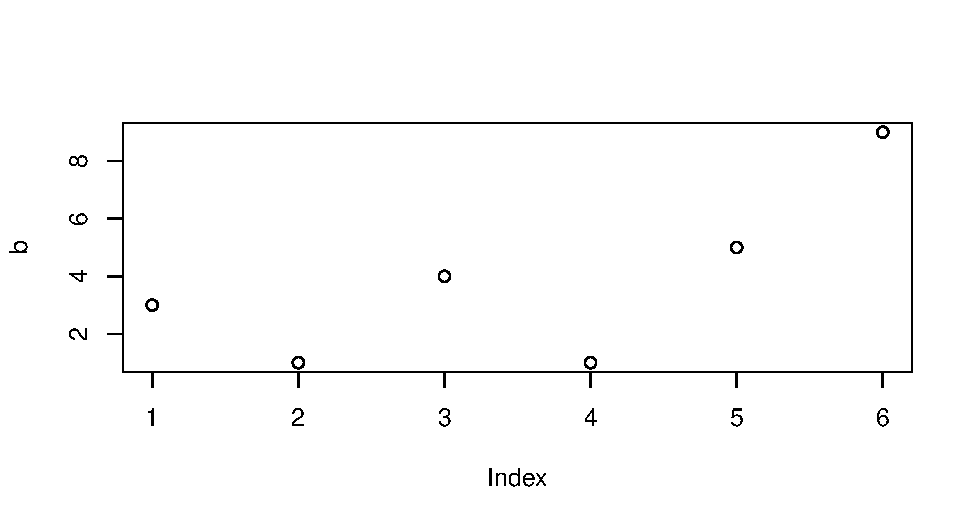
\includegraphics{R-anvisningar_files/figure-latex/unnamed-chunk-11-1} \end{center}

som ger en simpel graf, och

\begin{Shaded}
\begin{Highlighting}[]
\FunctionTok{sqrt}\NormalTok{(b)}
\end{Highlighting}
\end{Shaded}

\begin{verbatim}
## [1] 1.732051 1.000000 2.000000 1.000000 2.236068 3.000000
\end{verbatim}

som beräknar kvadratroten för varje element i vektorn.

Vid konstruktionen av vektorn användes också en grundläggande funktion - funktionen \texttt{c} som tar en serie värden och skapar en sammanhängande vektor av värden.

Alla R-funktioner har en tillhörande hjälpfil som kan plockas fram genom att skriva frågetecken följt av funktionsnamnet, t.ex. \texttt{?sum}. Från hjälpfilen får man att \texttt{sum} tar numeriska vektorer som ingående värde och beräknar summan. Man kan styra funktionens beteende genom att sätta ett argument \texttt{na.rm} (vilket här styr hur funktionen hanterar saknade värden). Som illustration kan man titta på

\begin{Shaded}
\begin{Highlighting}[]
\NormalTok{b }\OtherTok{\textless{}{-}} \FunctionTok{c}\NormalTok{(}\DecValTok{3}\NormalTok{, }\DecValTok{1}\NormalTok{, }\DecValTok{4}\NormalTok{, }\DecValTok{1}\NormalTok{, }\DecValTok{5}\NormalTok{, }\DecValTok{9}\NormalTok{, }\ConstantTok{NA}\NormalTok{)  }\CommentTok{\# Lägger till ett saknat värde}
\FunctionTok{sum}\NormalTok{(b)                        }\CommentTok{\# na.rm = FALSE är grundinställning}
\end{Highlighting}
\end{Shaded}

\begin{verbatim}
## [1] NA
\end{verbatim}

\begin{Shaded}
\begin{Highlighting}[]
\FunctionTok{sum}\NormalTok{(b, }\AttributeTok{na.rm =} \ConstantTok{TRUE}\NormalTok{)          }\CommentTok{\# na.rm sätts till TRUE}
\end{Highlighting}
\end{Shaded}

\begin{verbatim}
## [1] 23
\end{verbatim}

Det första försöket \texttt{sum(b)} ger utfallet \texttt{NA}, men om man sätter \texttt{na.rm\ =\ TRUE} beräknas summan efter att det saknade värdet plockats bort. Notera också att skript kan kommenteras med \texttt{\#}.

\hypertarget{sekvenser-av-funktioner}{%
\section{Sekvenser av funktioner}\label{sekvenser-av-funktioner}}

Ofta vill man genomföra flera operationer på ett objekt. Man behöver då genomföra en sekvens av funktionssteg. Säg till exempel att man har värdena \[(-4, -2, -1, 1, 2, 4)\] och vill ta absolutvärde (vilket gör negativa tal till motsvarande positiva tal) och sedan summera.
Den typen av sekvenser kan genomföras på ett par olika sätt. Ett första sätt är att spara resultatet i varje steg och sedan använda utfallet i nästa steg:

\begin{Shaded}
\begin{Highlighting}[]
\NormalTok{c }\OtherTok{\textless{}{-}} \FunctionTok{c}\NormalTok{(}\SpecialCharTok{{-}}\DecValTok{4}\NormalTok{, }\SpecialCharTok{{-}}\DecValTok{2}\NormalTok{, }\SpecialCharTok{{-}}\DecValTok{1}\NormalTok{, }\DecValTok{1}\NormalTok{, }\DecValTok{2}\NormalTok{, }\DecValTok{4}\NormalTok{)}
\NormalTok{c }\OtherTok{\textless{}{-}} \FunctionTok{abs}\NormalTok{(c)}
\FunctionTok{sum}\NormalTok{(c)}
\end{Highlighting}
\end{Shaded}

\begin{verbatim}
## [1] 14
\end{verbatim}

Här skapas ett objekt \texttt{c} som innehåller en vektor där några tal är negativa. I nästa rad används \texttt{abs} för att skapa absolutvärden. Slutligen summeras absolutvärdena med \texttt{sum}.
Notera för övrigt att det är möjligt att skapa ett objekt med namnet \texttt{c} trots att det redan är namnet på en funktion - R förstår ur sammanhanget vilket objekt som behövs.

Ett alternativ är att skriva en senare funktion \emph{runt} en tidigare funktion. Det fungerar för att R utvärderar funktioner inifrån-ut. Med samma exempel som tidigare får man

\begin{Shaded}
\begin{Highlighting}[]
\FunctionTok{sum}\NormalTok{(}\FunctionTok{abs}\NormalTok{(}\FunctionTok{c}\NormalTok{(}\SpecialCharTok{{-}}\DecValTok{4}\NormalTok{, }\SpecialCharTok{{-}}\DecValTok{2}\NormalTok{, }\SpecialCharTok{{-}}\DecValTok{1}\NormalTok{, }\DecValTok{1}\NormalTok{, }\DecValTok{2}\NormalTok{, }\DecValTok{4}\NormalTok{)))}
\end{Highlighting}
\end{Shaded}

\begin{verbatim}
## [1] 14
\end{verbatim}

Den här typen av skrivning kan spara plats men blir snabbt svårläst.

Ett sista alternativ är att använda en så kallad \emph{pipe} (namnet kommer från att en sekvens funktioner kallas en \emph{pipeline}). En pipe skrivs \texttt{\%\textgreater{}\%} och tar utfallet av en funktion till vänster och sänder till en funktion till höger. Språkligt kan pipen utläsas \emph{och sen}. Funktionen kan laddas genom att ladda paketet \texttt{tidyverse}. Med samma exempel som tidigare kan vi skriva

\begin{Shaded}
\begin{Highlighting}[]
\FunctionTok{library}\NormalTok{(tidyverse)}

\FunctionTok{c}\NormalTok{(}\SpecialCharTok{{-}}\DecValTok{4}\NormalTok{, }\SpecialCharTok{{-}}\DecValTok{2}\NormalTok{, }\SpecialCharTok{{-}}\DecValTok{1}\NormalTok{, }\DecValTok{1}\NormalTok{, }\DecValTok{2}\NormalTok{, }\DecValTok{4}\NormalTok{) }\SpecialCharTok{\%\textgreater{}\%}  \CommentTok{\# Skapa en datamängd och sen}
  \FunctionTok{abs}\NormalTok{() }\SpecialCharTok{\%\textgreater{}\%}                 \CommentTok{\# ta absolutvärden, och sen}
  \FunctionTok{sum}\NormalTok{()                     }\CommentTok{\# beräkna summan.}
\end{Highlighting}
\end{Shaded}

\begin{verbatim}
## [1] 14
\end{verbatim}

\hypertarget{dataimport}{%
\chapter{Dataimport}\label{dataimport}}

Det första praktiska steget i en statistisk analys är att importera data. I R kan det göras genom att direkt skriva in sin data och spara som ett nytt objekt, men ett bättre och vanligare sätt är att importera sin data från en extern fil eller databas. Om man arbetar med små datamängder har man ofta sin data i en excelfil.

Som exempel används här följande data från ett försök på purjolök.

\begin{table}
\centering
\begin{tabular}[t]{rrrr}
\toprule
Vecka & Behandling & Vikt & N\\
\midrule
7 & 0 & 232 & 2.63\\
7 & 0 & 161 & 2.90\\
7 & 0 & 148 & 2.99\\
7 & 1 & 368 & 3.54\\
7 & 1 & 218 & 3.30\\
\addlinespace
7 & 1 & 257 & 2.85\\
11 & 0 & 1633 & 1.53\\
11 & 0 & 2213 & 1.90\\
11 & 0 & 972 & NA\\
11 & 1 & 2560 & 2.58\\
\addlinespace
11 & 1 & 2430 & NA\\
11 & 1 & 855 & NA\\
\bottomrule
\end{tabular}
\end{table}

Notera att det finns saknade värden i kolumnen N.

\hypertarget{direkt-inskrivning-av-data}{%
\section{Direkt inskrivning av data}\label{direkt-inskrivning-av-data}}

I ett tidigare exempel användes funktionen \texttt{c} för att skapa en vektor av data. En datatabell (en \texttt{data.frame} i R) skapas genom funktionen \texttt{data.frame} följt av namngivna vektorer. Exempeldata kan skrivas in genom föjande.

\begin{Shaded}
\begin{Highlighting}[]
\NormalTok{dat }\OtherTok{\textless{}{-}} \FunctionTok{data.frame}\NormalTok{(}\AttributeTok{Vecka =} \FunctionTok{c}\NormalTok{(}\DecValTok{7}\NormalTok{, }\DecValTok{7}\NormalTok{, }\DecValTok{7}\NormalTok{, }\DecValTok{7}\NormalTok{, }\DecValTok{7}\NormalTok{, }\DecValTok{7}\NormalTok{, }
                            \DecValTok{11}\NormalTok{, }\DecValTok{11}\NormalTok{, }\DecValTok{11}\NormalTok{, }\DecValTok{11}\NormalTok{, }\DecValTok{11}\NormalTok{, }\DecValTok{11}\NormalTok{),}
                  \AttributeTok{Behandling =} \FunctionTok{c}\NormalTok{(}\DecValTok{0}\NormalTok{,}\DecValTok{0}\NormalTok{,}\DecValTok{0}\NormalTok{,}\DecValTok{1}\NormalTok{,}\DecValTok{1}\NormalTok{,}\DecValTok{1}\NormalTok{,}\DecValTok{0}\NormalTok{,}\DecValTok{0}\NormalTok{,}\DecValTok{0}\NormalTok{,}\DecValTok{1}\NormalTok{,}\DecValTok{1}\NormalTok{,}\DecValTok{1}\NormalTok{),}
                  \AttributeTok{Vikt =} \FunctionTok{c}\NormalTok{(}\DecValTok{232}\NormalTok{, }\DecValTok{161}\NormalTok{, }\DecValTok{148}\NormalTok{, }\DecValTok{368}\NormalTok{, }\DecValTok{218}\NormalTok{, }\DecValTok{257}\NormalTok{, }
                           \DecValTok{1633}\NormalTok{, }\DecValTok{2213}\NormalTok{, }\DecValTok{972}\NormalTok{, }\DecValTok{2560}\NormalTok{, }\DecValTok{2430}\NormalTok{, }\DecValTok{855}\NormalTok{),}
                  \AttributeTok{N =} \FunctionTok{c}\NormalTok{(}\FloatTok{2.63}\NormalTok{, }\FloatTok{2.90}\NormalTok{, }\FloatTok{2.99}\NormalTok{, }\FloatTok{3.54}\NormalTok{, }\FloatTok{3.30}\NormalTok{, }
                        \FloatTok{2.85}\NormalTok{, }\FloatTok{1.53}\NormalTok{, }\FloatTok{1.90}\NormalTok{, }\ConstantTok{NA}\NormalTok{, }\FloatTok{2.58}\NormalTok{, }\ConstantTok{NA}\NormalTok{, }\ConstantTok{NA}\NormalTok{))}

\NormalTok{dat}
\end{Highlighting}
\end{Shaded}

\begin{verbatim}
##    Vecka Behandling Vikt    N
## 1      7          0  232 2.63
## 2      7          0  161 2.90
## 3      7          0  148 2.99
## 4      7          1  368 3.54
## 5      7          1  218 3.30
## 6      7          1  257 2.85
## 7     11          0 1633 1.53
## 8     11          0 2213 1.90
## 9     11          0  972   NA
## 10    11          1 2560 2.58
## 11    11          1 2430   NA
## 12    11          1  855   NA
\end{verbatim}

Radbrytningar och blanksteg är oviktiga i R, och används bara för läsbarhet här. Saknade värden skrivs in som \texttt{NA} för \emph{not available}.

\hypertarget{import-fruxe5n-en-extern-fil}{%
\section{Import från en extern fil}\label{import-fruxe5n-en-extern-fil}}

Inskrivning av värden är ofta tidskrävande och kan lätt leda till misstag. Det är därför mycket vanligare att data läses in från en extern fil. Det finns en mängd funktioner för dataimport och det exakta valet av funktion beror på vilken typ av fil datan är sparad i. Det vanligaste filformatet för mindre datamängder är Excel. En excelfil kan läsas med \texttt{read\_excel} från paketet \texttt{readxl}.

\begin{Shaded}
\begin{Highlighting}[]
\FunctionTok{library}\NormalTok{(readxl)}
\NormalTok{dat }\OtherTok{\textless{}{-}} \FunctionTok{read\_excel}\NormalTok{(}\StringTok{"Data/Purjolök.xlsx"}\NormalTok{)}
\NormalTok{dat}
\end{Highlighting}
\end{Shaded}

\begin{verbatim}
## # A tibble: 12 x 4
##    Vecka Behandling  Vikt     N
##    <dbl>      <dbl> <dbl> <dbl>
##  1     7          0   232  2.63
##  2     7          0   161  2.9 
##  3     7          0   148  2.99
##  4     7          1   368  3.54
##  5     7          1   218  3.3 
##  6     7          1   257  2.85
##  7    11          0  1633  1.53
##  8    11          0  2213  1.9 
##  9    11          0   972 NA   
## 10    11          1  2560  2.58
## 11    11          1  2430 NA   
## 12    11          1   855 NA
\end{verbatim}

För att identifiera en fil behövs filens namn och placering. När man arbetar i R finns ett \emph{working directory}, en mapp på datorn som R-session för tillfället är kopplad till. Man kan se sitt \emph{working directory} genom att titta längst upp i konsollfönstret eller genom att köra \texttt{getwd()}. Ett filnamn kan anges relativt sessionens \emph{working directory}. Om man till exempel vill importera en fil som ligger i \emph{working directory} kan man ange filens namn direkt. I exemplet ovan låg excelfilen i en mapp \emph{Data} - filen måste därför anges som \texttt{Data/Purjolök.xlsx}.

Notera också att utskriften av den importerade datan inte ser likadan ut som utskriften av den inskrivna datan. Det beror på att \texttt{read\_excel} importerat datan som en \emph{tibble} - ett dataformat som har lite mer avancerade egenskaper är det ursprungliga dataformatet \texttt{data.frame}, till exempel ger en utskriven \emph{tibble} information om tabellens storlek och kolumnernas datatyper.

\hypertarget{beskrivande-statistik}{%
\chapter{Beskrivande statistik}\label{beskrivande-statistik}}

R och dess tilläggspaket innehåller funktioner för att sammanfatta och illustrera en datamängd. Detta avsnitt behandlar funktioner för att filtrera ut intressanta observationer, välja ut intressanta variabler, beräkna sammanfattande mått (som medelvärde, median och standardavvikelse), och konstruera och tolka grafer.

\hypertarget{datamuxe4ngd}{%
\section{Datamängd}\label{datamuxe4ngd}}

Som exempel används data från \emph{Gapminder} - en stiftelse med mål att sprida information om ekonomisk utveckling och hälsa, grundad av Hans Rosling (1948-2017). Datamängden finns tillgänglig i R-paketet \texttt{gapminder}.

\begin{Shaded}
\begin{Highlighting}[]
\FunctionTok{install.packages}\NormalTok{(}\StringTok{"gapminder"}\NormalTok{) }\CommentTok{\# Behöver bara köras första gången}
\FunctionTok{library}\NormalTok{(gapminder)}
\end{Highlighting}
\end{Shaded}

Efter att paketet laddas med \texttt{library(gapminder)} är datan tillgänglig under namnet \texttt{gapminder}. Man kan skriva ut de första raderna genom

\begin{Shaded}
\begin{Highlighting}[]
\NormalTok{gapminder}
\end{Highlighting}
\end{Shaded}

\begin{verbatim}
## # A tibble: 1,704 x 6
##    country     continent  year lifeExp      pop gdpPercap
##    <fct>       <fct>     <int>   <dbl>    <int>     <dbl>
##  1 Afghanistan Asia       1952    28.8  8425333      779.
##  2 Afghanistan Asia       1957    30.3  9240934      821.
##  3 Afghanistan Asia       1962    32.0 10267083      853.
##  4 Afghanistan Asia       1967    34.0 11537966      836.
##  5 Afghanistan Asia       1972    36.1 13079460      740.
##  6 Afghanistan Asia       1977    38.4 14880372      786.
##  7 Afghanistan Asia       1982    39.9 12881816      978.
##  8 Afghanistan Asia       1987    40.8 13867957      852.
##  9 Afghanistan Asia       1992    41.7 16317921      649.
## 10 Afghanistan Asia       1997    41.8 22227415      635.
## # ... with 1,694 more rows
\end{verbatim}

Datan anger förväntad medellivslängd, populationsstorlek och bnp per capita, per land och år (vart femte år från 1952 till 2007).

\hypertarget{filtrering-av-rader-och-selektion-av-kolumner}{%
\section{Filtrering av rader och selektion av kolumner}\label{filtrering-av-rader-och-selektion-av-kolumner}}

En vanlig operation på en tabell är att göra ett urval - antingen ett urval av rader (t.ex. ett visst land eller år), vilket kallas \emph{filtrering} eller ett urval av variabler (t.ex. år och population), vilket kallas \emph{selektion}.
Det finns flera olika sätt att göra ett urval i R.
Det traditionella sättet är att använda index inom hakparenteser (t.ex. \texttt{gapminder{[}4,\ 2{]}} för fjärde raden, andra kolumnen) eller dollartecken för specifika kolumner (t.ex. \texttt{gapminder\$pop} för befolkningskolumnen).
Här fokuseras dock på hur det kan göras med funktionerna \texttt{filter} och \texttt{select} från paketet \texttt{tidyverse}.

För att filtrera på ett givet land kan använda pipe-funktionen från datan till en filter-funktion, t.ex.

\begin{Shaded}
\begin{Highlighting}[]
\NormalTok{gapminder }\SpecialCharTok{\%\textgreater{}\%}                 \CommentTok{\# Ta gapminder{-}datan och sen}
  \FunctionTok{filter}\NormalTok{(country }\SpecialCharTok{==} \StringTok{"Sweden"}\NormalTok{) }\CommentTok{\# filtrera för specifikt land}
\end{Highlighting}
\end{Shaded}

\begin{verbatim}
## # A tibble: 12 x 6
##    country continent  year lifeExp     pop gdpPercap
##    <fct>   <fct>     <int>   <dbl>   <int>     <dbl>
##  1 Sweden  Europe     1952    71.9 7124673     8528.
##  2 Sweden  Europe     1957    72.5 7363802     9912.
##  3 Sweden  Europe     1962    73.4 7561588    12329.
##  4 Sweden  Europe     1967    74.2 7867931    15258.
##  5 Sweden  Europe     1972    74.7 8122293    17832.
##  6 Sweden  Europe     1977    75.4 8251648    18856.
##  7 Sweden  Europe     1982    76.4 8325260    20667.
##  8 Sweden  Europe     1987    77.2 8421403    23587.
##  9 Sweden  Europe     1992    78.2 8718867    23880.
## 10 Sweden  Europe     1997    79.4 8897619    25267.
## 11 Sweden  Europe     2002    80.0 8954175    29342.
## 12 Sweden  Europe     2007    80.9 9031088    33860.
\end{verbatim}

Inom filter-funktionen anges ett logisk villkor \texttt{country\ ==\ "Sweden"} och utfallet är de rader där villkoret är sant. Notera de dubbla likhetstecknen - de måste användas för ett logisk villkor eftersom enkelt likhetstecken används för att skapa objekt och sätta funktionsargument. Om man vill välja flera länder kan man använda funktionen \texttt{\%in\%} på ett liknande sätt.

\begin{Shaded}
\begin{Highlighting}[]
\NormalTok{gapminder }\SpecialCharTok{\%\textgreater{}\%} 
  \FunctionTok{filter}\NormalTok{(country }\SpecialCharTok{\%in\%} \FunctionTok{c}\NormalTok{(}\StringTok{"Sweden"}\NormalTok{, }\StringTok{"Denmark"}\NormalTok{))}
\end{Highlighting}
\end{Shaded}

\begin{verbatim}
## # A tibble: 24 x 6
##    country continent  year lifeExp     pop gdpPercap
##    <fct>   <fct>     <int>   <dbl>   <int>     <dbl>
##  1 Denmark Europe     1952    70.8 4334000     9692.
##  2 Denmark Europe     1957    71.8 4487831    11100.
##  3 Denmark Europe     1962    72.4 4646899    13583.
##  4 Denmark Europe     1967    73.0 4838800    15937.
##  5 Denmark Europe     1972    73.5 4991596    18866.
##  6 Denmark Europe     1977    74.7 5088419    20423.
##  7 Denmark Europe     1982    74.6 5117810    21688.
##  8 Denmark Europe     1987    74.8 5127024    25116.
##  9 Denmark Europe     1992    75.3 5171393    26407.
## 10 Denmark Europe     1997    76.1 5283663    29804.
## # ... with 14 more rows
\end{verbatim}

och om man vill ha mer än ett villkor kan man rada dem i filter-funktionen eller ha flera filter-steg:

\begin{Shaded}
\begin{Highlighting}[]
\NormalTok{gapminder }\SpecialCharTok{\%\textgreater{}\%} 
  \FunctionTok{filter}\NormalTok{(country }\SpecialCharTok{\%in\%} \FunctionTok{c}\NormalTok{(}\StringTok{"Sweden"}\NormalTok{, }\StringTok{"Denmark"}\NormalTok{),}
\NormalTok{         year }\SpecialCharTok{==} \DecValTok{1987}\NormalTok{)}
\end{Highlighting}
\end{Shaded}

\begin{verbatim}
## # A tibble: 2 x 6
##   country continent  year lifeExp     pop gdpPercap
##   <fct>   <fct>     <int>   <dbl>   <int>     <dbl>
## 1 Denmark Europe     1987    74.8 5127024    25116.
## 2 Sweden  Europe     1987    77.2 8421403    23587.
\end{verbatim}

alternativt

\begin{Shaded}
\begin{Highlighting}[]
\NormalTok{gapminder }\SpecialCharTok{\%\textgreater{}\%} 
  \FunctionTok{filter}\NormalTok{(country }\SpecialCharTok{\%in\%} \FunctionTok{c}\NormalTok{(}\StringTok{"Sweden"}\NormalTok{, }\StringTok{"Denmark"}\NormalTok{)) }\SpecialCharTok{\%\textgreater{}\%} 
  \FunctionTok{filter}\NormalTok{(year }\SpecialCharTok{==} \DecValTok{1987}\NormalTok{)}
\end{Highlighting}
\end{Shaded}

\begin{verbatim}
## # A tibble: 2 x 6
##   country continent  year lifeExp     pop gdpPercap
##   <fct>   <fct>     <int>   <dbl>   <int>     <dbl>
## 1 Denmark Europe     1987    74.8 5127024    25116.
## 2 Sweden  Europe     1987    77.2 8421403    23587.
\end{verbatim}

Om man istället vill göra ett urval av kolumner kan man använda \texttt{select}. Som argument anges de kolumner man vill välja, t.ex.

\begin{Shaded}
\begin{Highlighting}[]
\NormalTok{gapminder }\SpecialCharTok{\%\textgreater{}\%} 
  \FunctionTok{select}\NormalTok{(country, pop)}
\end{Highlighting}
\end{Shaded}

\begin{verbatim}
## # A tibble: 1,704 x 2
##    country          pop
##    <fct>          <int>
##  1 Afghanistan  8425333
##  2 Afghanistan  9240934
##  3 Afghanistan 10267083
##  4 Afghanistan 11537966
##  5 Afghanistan 13079460
##  6 Afghanistan 14880372
##  7 Afghanistan 12881816
##  8 Afghanistan 13867957
##  9 Afghanistan 16317921
## 10 Afghanistan 22227415
## # ... with 1,694 more rows
\end{verbatim}

Som avslutning ges ett lite mer komplicerat exempel på ett urval av land, kontinent och befolkning för länder utanför Europa som 2002 hade en befolkning över 100 miljoner

\begin{Shaded}
\begin{Highlighting}[]
\NormalTok{gapminder }\SpecialCharTok{\%\textgreater{}\%}                     \CommentTok{\# Ta datan och sen}
  \FunctionTok{filter}\NormalTok{(continent }\SpecialCharTok{!=} \StringTok{"Europe"}\NormalTok{,   }\CommentTok{\# filtrera på kontinent ej lika med (!=) Europa,}
\NormalTok{         year }\SpecialCharTok{==} \DecValTok{2002}\NormalTok{,            }\CommentTok{\# år lika med 2002,}
\NormalTok{         pop }\SpecialCharTok{\textgreater{}} \DecValTok{100000000}\NormalTok{) }\SpecialCharTok{\%\textgreater{}\%}     \CommentTok{\# befolkning över 100 mil, och sen}
  \FunctionTok{select}\NormalTok{(country, continent, pop) }\CommentTok{\# selektera på land, kontinent och befolkning}
\end{Highlighting}
\end{Shaded}

\begin{verbatim}
## # A tibble: 10 x 3
##    country       continent        pop
##    <fct>         <fct>          <int>
##  1 Bangladesh    Asia       135656790
##  2 Brazil        Americas   179914212
##  3 China         Asia      1280400000
##  4 India         Asia      1034172547
##  5 Indonesia     Asia       211060000
##  6 Japan         Asia       127065841
##  7 Mexico        Americas   102479927
##  8 Nigeria       Africa     119901274
##  9 Pakistan      Asia       153403524
## 10 United States Americas   287675526
\end{verbatim}

\hypertarget{transformationer-av-variabler}{%
\section{Transformationer av variabler}\label{transformationer-av-variabler}}

Variabler kan omräknas och nya variabler kan skapas med \texttt{mutate}-funktionen. I gapminder-datan finns befolkning och bnp per capita, så det är naturligt att beräkna total bnp som produkten av de två variablerna genom multiplikation.

\begin{Shaded}
\begin{Highlighting}[]
\NormalTok{gapminder }\OtherTok{\textless{}{-}}\NormalTok{ gapminder }\SpecialCharTok{\%\textgreater{}\%} 
  \FunctionTok{mutate}\NormalTok{(}\AttributeTok{gdptotal =}\NormalTok{ gdpPercap }\SpecialCharTok{*}\NormalTok{ pop)}
\end{Highlighting}
\end{Shaded}

Den inledande delen med \texttt{gapminder\ \textless{}-} gör så att utfallet av beräkningen sparas i gapminder-datan.
Vi kan skriva ut objektet och se resultatet av beräkningen:

\begin{Shaded}
\begin{Highlighting}[]
\NormalTok{gapminder}
\end{Highlighting}
\end{Shaded}

\begin{verbatim}
## # A tibble: 1,704 x 7
##    country     continent  year lifeExp      pop gdpPercap     gdptotal
##    <fct>       <fct>     <int>   <dbl>    <int>     <dbl>        <dbl>
##  1 Afghanistan Asia       1952    28.8  8425333      779.  6567086330.
##  2 Afghanistan Asia       1957    30.3  9240934      821.  7585448670.
##  3 Afghanistan Asia       1962    32.0 10267083      853.  8758855797.
##  4 Afghanistan Asia       1967    34.0 11537966      836.  9648014150.
##  5 Afghanistan Asia       1972    36.1 13079460      740.  9678553274.
##  6 Afghanistan Asia       1977    38.4 14880372      786. 11697659231.
##  7 Afghanistan Asia       1982    39.9 12881816      978. 12598563401.
##  8 Afghanistan Asia       1987    40.8 13867957      852. 11820990309.
##  9 Afghanistan Asia       1992    41.7 16317921      649. 10595901589.
## 10 Afghanistan Asia       1997    41.8 22227415      635. 14121995875.
## # ... with 1,694 more rows
\end{verbatim}

\hypertarget{sammanfattande-statistik}{%
\section{Sammanfattande statistik}\label{sammanfattande-statistik}}

För att presentera insamlad data på ett tolkningsbart sätt används sammanfattande mått såsom summor, medelvärden, medianer och standardavvikelser.
Den typen av beräkningar kan göras som ett nytt steg i en pipe med hjälp av funktionen \texttt{summarise}. Om man kombinerar \texttt{summarise} med funktionen \texttt{group\_by} kan man dessutom summera efter en indelning given av en annan variabel. En beräkning av total befolkningsmängd per år kan till exempel ges av

\begin{Shaded}
\begin{Highlighting}[]
\NormalTok{gapminder }\SpecialCharTok{\%\textgreater{}\%}                           \CommentTok{\# Ta datan och sen}
  \FunctionTok{group\_by}\NormalTok{(year) }\SpecialCharTok{\%\textgreater{}\%}                    \CommentTok{\# gruppera efter år och sen}
  \FunctionTok{summarise}\NormalTok{(}\AttributeTok{Totalbefolkning =} \FunctionTok{sum}\NormalTok{(pop) }\SpecialCharTok{/} \FloatTok{1e9}\NormalTok{) }\CommentTok{\# summera per grupp}
\end{Highlighting}
\end{Shaded}

\begin{verbatim}
## # A tibble: 12 x 2
##     year Totalbefolkning
##    <int>           <dbl>
##  1  1952            2.41
##  2  1957            2.66
##  3  1962            2.90
##  4  1967            3.22
##  5  1972            3.58
##  6  1977            3.93
##  7  1982            4.29
##  8  1987            4.69
##  9  1992            5.11
## 10  1997            5.52
## 11  2002            5.89
## 12  2007            6.25
\end{verbatim}

I det sista steget skapas en variabel \emph{Totalbefolkning} som ges av summan av den ursprungliga variabeln \emph{pop}.

Funktionerna \texttt{summarise\_at} och \texttt{summarise\_all} kan användas för att summera flera variabler i ett steg. Man kan också ange mer än en funktion, om man vill beräkna flera olika mått.

\begin{Shaded}
\begin{Highlighting}[]
\NormalTok{gapminder }\SpecialCharTok{\%\textgreater{}\%} 
  \FunctionTok{filter}\NormalTok{(year }\SpecialCharTok{==} \DecValTok{2007}\NormalTok{) }\SpecialCharTok{\%\textgreater{}\%} 
  \FunctionTok{group\_by}\NormalTok{(continent) }\SpecialCharTok{\%\textgreater{}\%} 
  \FunctionTok{summarise\_at}\NormalTok{(}\FunctionTok{c}\NormalTok{(}\StringTok{"lifeExp"}\NormalTok{, }\StringTok{"pop"}\NormalTok{), }\FunctionTok{c}\NormalTok{(mean, sd))}
\end{Highlighting}
\end{Shaded}

\begin{verbatim}
## # A tibble: 5 x 5
##   continent lifeExp_fn1    pop_fn1 lifeExp_fn2    pop_fn2
##   <fct>           <dbl>      <dbl>       <dbl>      <dbl>
## 1 Africa           54.8  17875763.       9.63   24917726.
## 2 Americas         73.6  35954847.       4.44   68833781.
## 3 Asia             70.7 115513752.       7.96  289673399.
## 4 Europe           77.6  19536618.       2.98   23624744.
## 5 Oceania          80.7  12274974.       0.729  11538855.
\end{verbatim}

Kolumnerna för förväntat medelllivslängd och befolkning sammanfattas med medelvärde och standardavvikelse för observationer från 2007.

\hypertarget{grafer}{%
\section{Grafer}\label{grafer}}

R har en mängd grundläggande funktioner för grafer. Ett enkelt spridningsdiagram kan till exempel skapas med

\begin{Shaded}
\begin{Highlighting}[]
\FunctionTok{plot}\NormalTok{(gapminder}\SpecialCharTok{$}\NormalTok{gdpPercap, gapminder}\SpecialCharTok{$}\NormalTok{lifeExp)}
\end{Highlighting}
\end{Shaded}

\begin{center}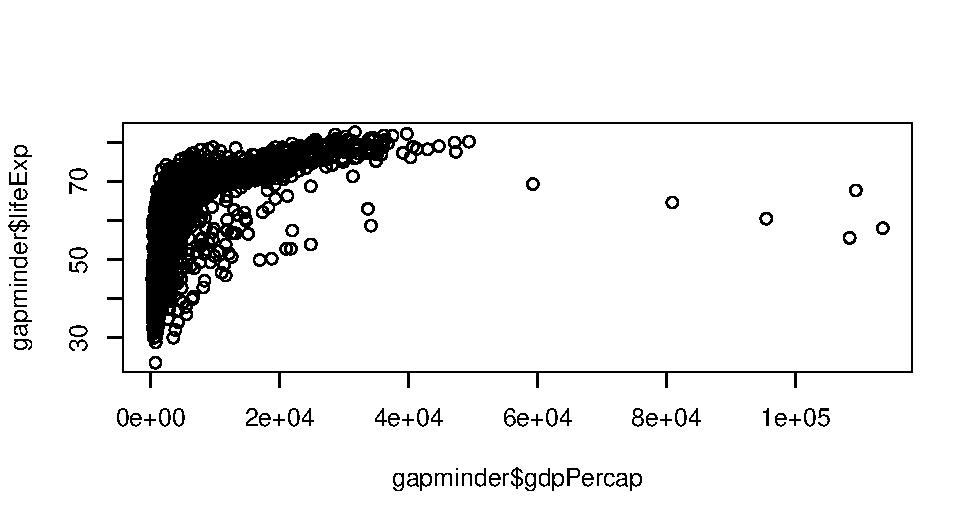
\includegraphics{R-anvisningar_files/figure-latex/unnamed-chunk-33-1} \end{center}

Tecknet \texttt{\$} används här för att välja en kolumn i en tabell.

För mer avancerade grafer används dock ofta funktioner ur Rs paketbibliotek. Här illustreras det mest populära - \texttt{ggplot2}. I \texttt{ggplot2} byggs grafer upp med tre grundläggande byggstenar:

\begin{itemize}
\tightlist
\item
  \emph{data}, informationen man vill visualisera,
\item
  \emph{aestethics}, en koppling mellan data och visuella element såsom grafens axlar, objekts storlek och färg,
\item
  \emph{geometries}, de geometriska former som visas i grafen.
\end{itemize}

En graf skrivs med en startfunktion \texttt{ggplot} som anger namnet på datan och grafens \emph{aestethics}, och därefter sätts geometriska element genom funktioner som börjar med \texttt{geom\_}. Ett spridningsdiagram kan t.ex. skapas med \texttt{geom\_point}.

\begin{Shaded}
\begin{Highlighting}[]
\FunctionTok{ggplot}\NormalTok{(gapminder, }\FunctionTok{aes}\NormalTok{(}\AttributeTok{x =}\NormalTok{ gdpPercap, }\AttributeTok{y =}\NormalTok{ lifeExp)) }\SpecialCharTok{+}
  \FunctionTok{geom\_point}\NormalTok{()}
\end{Highlighting}
\end{Shaded}

\begin{center}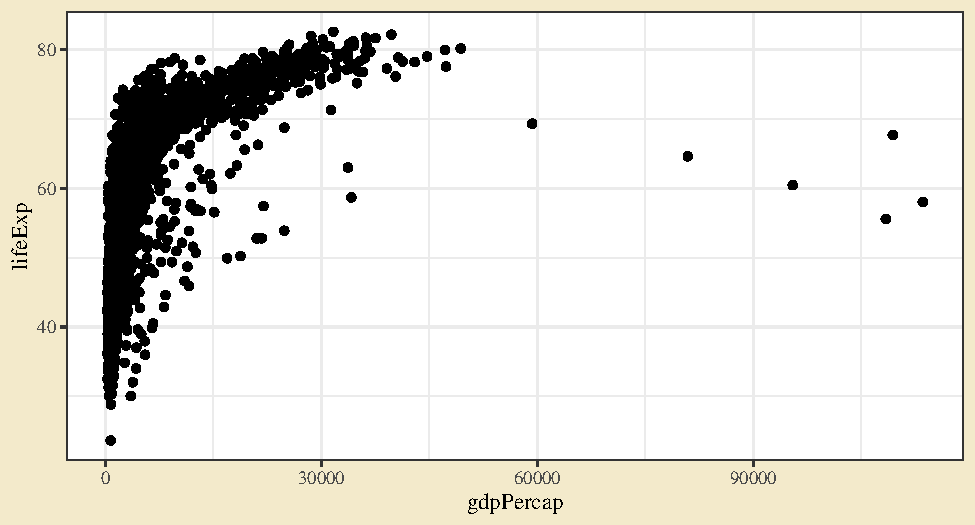
\includegraphics{R-anvisningar_files/figure-latex/unnamed-chunk-34-1} \end{center}

Grafen kan byggas ut genom att sätta \emph{aestethics} för färg och storlek. Man kan också dela en graf i småfönster med \texttt{facet\_wrap} och styra grafens utseende genom att sätta ett tema såsom \texttt{theme\_bw}.

\begin{Shaded}
\begin{Highlighting}[]
\FunctionTok{ggplot}\NormalTok{(gapminder, }\FunctionTok{aes}\NormalTok{(}\AttributeTok{x =} \FunctionTok{log}\NormalTok{(gdpPercap), }\AttributeTok{y =}\NormalTok{ lifeExp, }\AttributeTok{color =}\NormalTok{ continent, }\AttributeTok{size =}\NormalTok{ pop)) }\SpecialCharTok{+}
  \FunctionTok{geom\_point}\NormalTok{() }\SpecialCharTok{+}
  \FunctionTok{facet\_wrap}\NormalTok{(}\SpecialCharTok{\textasciitilde{}}\NormalTok{ year)}
\end{Highlighting}
\end{Shaded}

\begin{center}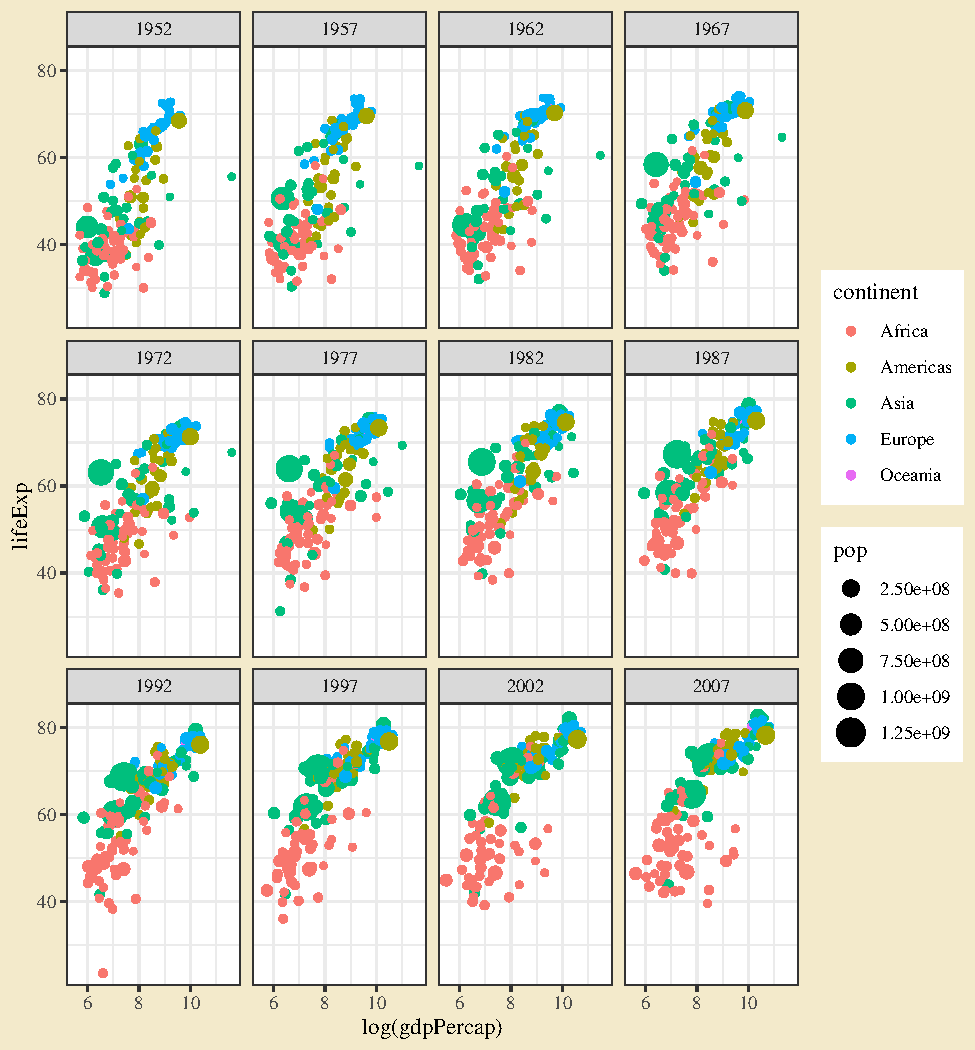
\includegraphics{R-anvisningar_files/figure-latex/unnamed-chunk-35-1} \end{center}

Här används dessutom log-transformerad bnp per capita för att få en jämnare fördelning i x-axeln.

Andra graftyper kan skapas med andra \texttt{geom\_}-funktioner. För ett linjediagram används \texttt{geom\_line}. De observationer som ska ge en specifik linje anges med \texttt{group} i \texttt{aes}-funktionen.

\begin{Shaded}
\begin{Highlighting}[]
\FunctionTok{ggplot}\NormalTok{(gapminder, }\FunctionTok{aes}\NormalTok{(}\AttributeTok{x =}\NormalTok{ year, }\AttributeTok{y =}\NormalTok{ lifeExp, }\AttributeTok{color =}\NormalTok{ continent, }\AttributeTok{group =}\NormalTok{ country)) }\SpecialCharTok{+}
  \FunctionTok{geom\_line}\NormalTok{()}
\end{Highlighting}
\end{Shaded}

\begin{center}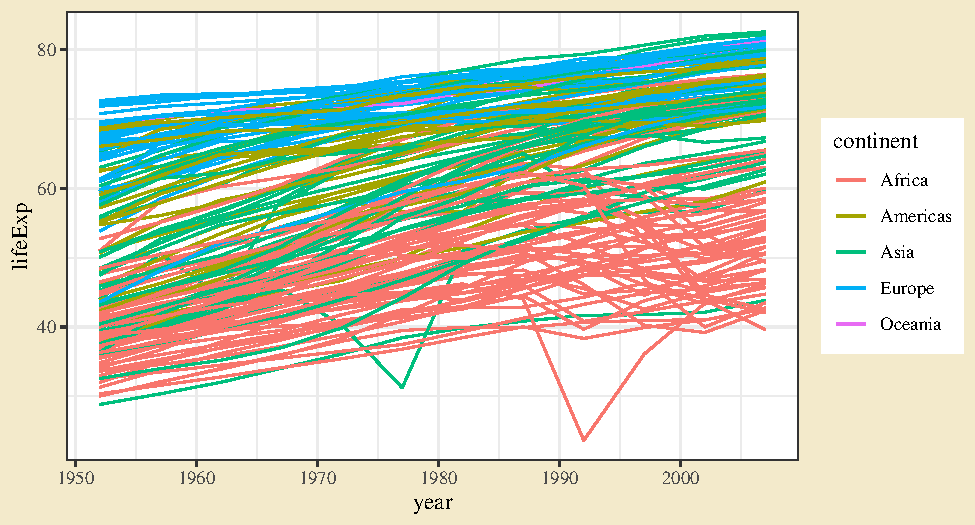
\includegraphics{R-anvisningar_files/figure-latex/unnamed-chunk-36-1} \end{center}

Stapeldiagram ges av \texttt{geom\_bar}. Om diagrammet ska visa ett urval av data kan man skriva grafen som sista steget i en längre pipe, t.ex.

\begin{Shaded}
\begin{Highlighting}[]
\NormalTok{gapminder }\SpecialCharTok{\%\textgreater{}\%} 
  \FunctionTok{filter}\NormalTok{(year }\SpecialCharTok{==} \DecValTok{2007}\NormalTok{) }\SpecialCharTok{\%\textgreater{}\%} 
  \FunctionTok{filter}\NormalTok{(}\FunctionTok{rank}\NormalTok{(}\SpecialCharTok{{-}}\NormalTok{pop) }\SpecialCharTok{\textless{}=} \DecValTok{20}\NormalTok{) }\SpecialCharTok{\%\textgreater{}\%} 
  \FunctionTok{ggplot}\NormalTok{(}\FunctionTok{aes}\NormalTok{(}\AttributeTok{x =}\NormalTok{ pop, }\AttributeTok{y =} \FunctionTok{reorder}\NormalTok{(country, pop), }\AttributeTok{fill =}\NormalTok{ continent)) }\SpecialCharTok{+}
  \FunctionTok{geom\_bar}\NormalTok{(}\AttributeTok{stat =} \StringTok{"identity"}\NormalTok{)}
\end{Highlighting}
\end{Shaded}

\begin{center}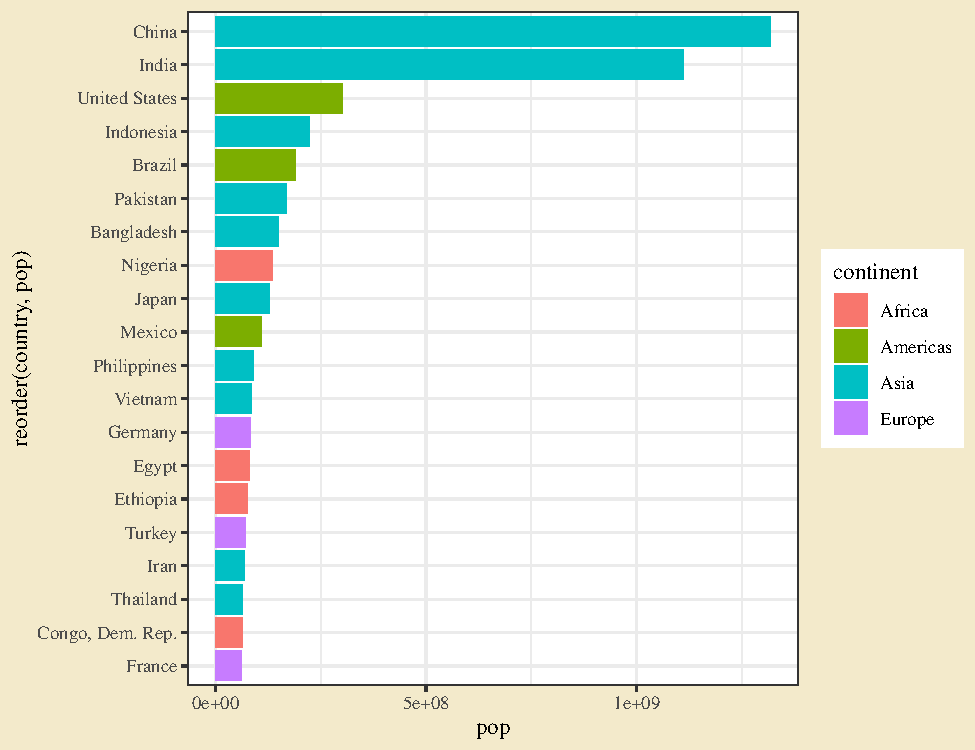
\includegraphics{R-anvisningar_files/figure-latex/unnamed-chunk-37-1} \end{center}

Här ger \texttt{rank(-pop)\ \textless{}=\ 20} att landets rang, dess värde i storleksordning, är minst 20, \texttt{reorder(country,\ pop)} att länder skrivs ut i grafen i storleksordning, och \texttt{stat\ =\ "identity"} att värdet för pop ska skrivas ut i grafen som det är (utan att transformeras).

\hypertarget{uxf6vningar}{%
\section{Övningar}\label{uxf6vningar}}

\begin{exercise}[Antal barn]
Antal barn per familj för 30 familjer är

\begin{table}
\centering
\begin{tabular}[t]{rrrrrrrrrr}
\toprule
4 & 3 & 0 & 0 & 0 & 1 & 5 & 2 & 2 & 8\\
3 & 1 & 0 & 1 & 2 & 1 & 1 & 4 & 1 & 0\\
2 & 2 & 3 & 0 & 4 & 1 & 5 & 1 & 1 & 3\\
\bottomrule
\end{tabular}
\end{table}

a. Sammanfatta materialet i en frekvenstabell och illustrera materialet med ett lämpligt diagram.

b. Beräkna genomsnittligt antal barn per familj.

c. Beräkna variansen.

d. Pröva att ändra sista värdet till 30 och se vad som händer med resultaten.
\end{exercise}

\begin{hypothesis}[Antal barn]
Datan kan illustreras med ett stapeldiagram och beskrivande statistik kan beräknas med lämpliga funktioner.

a.

\begin{Shaded}
\begin{Highlighting}[]
\NormalTok{dat }\OtherTok{\textless{}{-}} \FunctionTok{c}\NormalTok{(}\DecValTok{4}\NormalTok{,}\DecValTok{3}\NormalTok{,}\DecValTok{0}\NormalTok{,}\DecValTok{0}\NormalTok{,}\DecValTok{0}\NormalTok{,}\DecValTok{1}\NormalTok{,}\DecValTok{5}\NormalTok{,}\DecValTok{2}\NormalTok{,}\DecValTok{2}\NormalTok{,}\DecValTok{8}\NormalTok{,}\DecValTok{3}\NormalTok{,}\DecValTok{1}\NormalTok{,}\DecValTok{0}\NormalTok{,}\DecValTok{1}\NormalTok{,}\DecValTok{2}\NormalTok{,}\DecValTok{1}\NormalTok{,}\DecValTok{1}\NormalTok{,}\DecValTok{4}\NormalTok{,}\DecValTok{1}\NormalTok{,}\DecValTok{0}\NormalTok{,}\DecValTok{2}\NormalTok{,}\DecValTok{2}\NormalTok{,}\DecValTok{3}\NormalTok{,}\DecValTok{0}\NormalTok{,}\DecValTok{4}\NormalTok{,}\DecValTok{1}\NormalTok{,}\DecValTok{5}\NormalTok{,}\DecValTok{1}\NormalTok{,}\DecValTok{1}\NormalTok{,}\DecValTok{3}\NormalTok{)}
\FunctionTok{table}\NormalTok{(dat)}
\end{Highlighting}
\end{Shaded}

\begin{verbatim}
## dat
## 0 1 2 3 4 5 8 
## 6 9 5 4 3 2 1
\end{verbatim}

\begin{Shaded}
\begin{Highlighting}[]
\NormalTok{dat }\OtherTok{\textless{}{-}} \FunctionTok{tibble}\NormalTok{(}\StringTok{\textasciigrave{}}\AttributeTok{Antal barn}\StringTok{\textasciigrave{}} \OtherTok{=}\NormalTok{ dat)}
\FunctionTok{ggplot}\NormalTok{(dat, }\FunctionTok{aes}\NormalTok{(}\StringTok{\textasciigrave{}}\AttributeTok{Antal barn}\StringTok{\textasciigrave{}}\NormalTok{)) }\SpecialCharTok{+}
  \FunctionTok{geom\_bar}\NormalTok{() }\SpecialCharTok{+}
  \FunctionTok{scale\_x\_continuous}\NormalTok{(}\AttributeTok{breaks =} \DecValTok{0}\SpecialCharTok{:}\DecValTok{8}\NormalTok{) }\SpecialCharTok{+}
  \FunctionTok{scale\_y\_continuous}\NormalTok{(}\AttributeTok{breaks =} \DecValTok{0}\SpecialCharTok{:}\DecValTok{10}\NormalTok{) }\SpecialCharTok{+}
  \FunctionTok{ylab}\NormalTok{(}\StringTok{"Frekvens"}\NormalTok{) }\SpecialCharTok{+}
  \FunctionTok{theme}\NormalTok{(}\AttributeTok{panel.grid.minor =} \FunctionTok{element\_blank}\NormalTok{(),}
        \AttributeTok{panel.grid.major.x =} \FunctionTok{element\_blank}\NormalTok{())}
\end{Highlighting}
\end{Shaded}

\begin{center}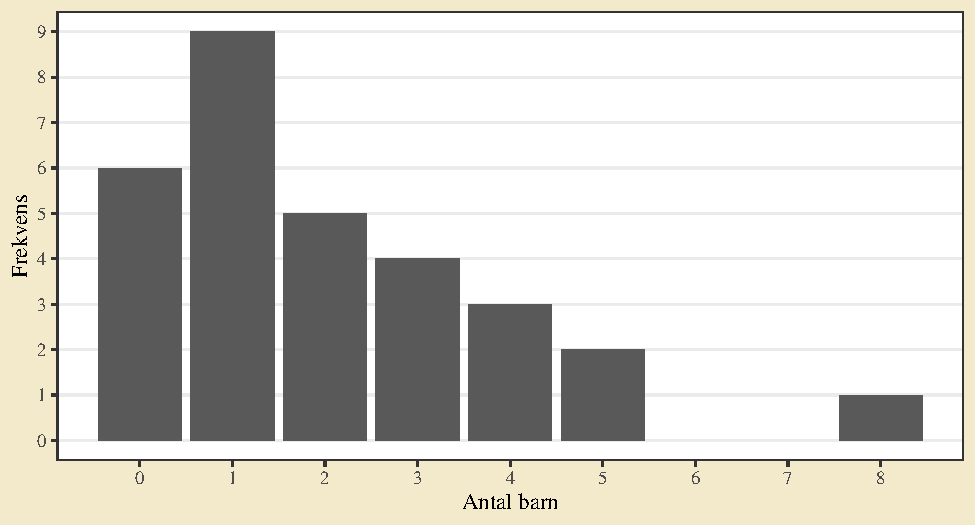
\includegraphics{R-anvisningar_files/figure-latex/unnamed-chunk-40-1} \end{center}

b.

\begin{Shaded}
\begin{Highlighting}[]
\NormalTok{dat }\SpecialCharTok{\%\textgreater{}\%} \FunctionTok{summarise\_all}\NormalTok{(}\FunctionTok{c}\NormalTok{(mean, median, var))}
\end{Highlighting}
\end{Shaded}

\begin{verbatim}
## # A tibble: 1 x 3
##     fn1   fn2   fn3
##   <dbl> <dbl> <dbl>
## 1  2.03   1.5  3.55
\end{verbatim}

c.

\begin{Shaded}
\begin{Highlighting}[]
\FunctionTok{var}\NormalTok{(dat}\SpecialCharTok{$}\StringTok{\textasciigrave{}}\AttributeTok{Antal barn}\StringTok{\textasciigrave{}}\NormalTok{)}
\end{Highlighting}
\end{Shaded}

\begin{verbatim}
## [1] 3.550575
\end{verbatim}

d.

\begin{Shaded}
\begin{Highlighting}[]
\NormalTok{dat}\SpecialCharTok{$}\StringTok{\textasciigrave{}}\AttributeTok{Antal barn}\StringTok{\textasciigrave{}}\NormalTok{[}\DecValTok{30}\NormalTok{] }\OtherTok{\textless{}{-}} \DecValTok{30} \CommentTok{\# Ändra trettionde värde till 30}
\NormalTok{dat }\SpecialCharTok{\%\textgreater{}\%} \FunctionTok{summarise\_all}\NormalTok{(}\FunctionTok{c}\NormalTok{(mean, median, var))}
\end{Highlighting}
\end{Shaded}

\begin{verbatim}
## # A tibble: 1 x 3
##     fn1   fn2   fn3
##   <dbl> <dbl> <dbl>
## 1  2.93   1.5  29.7
\end{verbatim}

Medelvärde ökar med ungefär 1, medianen är densamma (varför?) och variansen ökar kraftigt.
\end{hypothesis}

\begin{exercise}[Darwindata]
Följande data gäller längden (i tum) hos 15 stycken plantor som fortplantats genom självbefruktning:

\begin{table}
\centering
\begin{tabular}[t]{rrrrr}
\toprule
17.4 & 20.4 & 20.0 & 20.0 & 18.4\\
18.6 & 18.6 & 15.3 & 16.5 & 18.0\\
16.3 & 18.0 & 12.8 & 15.5 & 18.0\\
\bottomrule
\end{tabular}
\end{table}

a. Beräkna medelvärdet.

b. Beräkna medianen.

c. Beräkna variansen.

d. Beskriv fördelningen med ett histogram.

e. Beskriv fördelningen med ett lådagram.
\end{exercise}

\begin{hypothesis}[Darwindata]
Funktionen \texttt{summarise\_all} kan användas för att beräkna medelvärde, median och varians. Grafer kan konstrueras med \texttt{geom\_histogram} och \texttt{geom\_boxplot}.

\begin{Shaded}
\begin{Highlighting}[]
\NormalTok{dat }\OtherTok{\textless{}{-}} \FunctionTok{tibble}\NormalTok{(Längd }\OtherTok{=} \FunctionTok{c}\NormalTok{(}\DecValTok{174}\NormalTok{,}\DecValTok{204}\NormalTok{,}\DecValTok{200}\NormalTok{,}\DecValTok{200}\NormalTok{,}\DecValTok{184}\NormalTok{,}\DecValTok{186}\NormalTok{,}\DecValTok{186}\NormalTok{,}
                        \DecValTok{153}\NormalTok{,}\DecValTok{165}\NormalTok{,}\DecValTok{180}\NormalTok{,}\DecValTok{163}\NormalTok{,}\DecValTok{180}\NormalTok{,}\DecValTok{128}\NormalTok{,}\DecValTok{155}\NormalTok{,}\DecValTok{180}\NormalTok{))}
\NormalTok{dat }\SpecialCharTok{\%\textgreater{}\%} 
  \FunctionTok{summarise\_all}\NormalTok{(}\FunctionTok{c}\NormalTok{(mean, median, var))}
\end{Highlighting}
\end{Shaded}

\begin{verbatim}
## # A tibble: 1 x 3
##     fn1   fn2   fn3
##   <dbl> <dbl> <dbl>
## 1  176.   180  415.
\end{verbatim}

\begin{Shaded}
\begin{Highlighting}[]
\FunctionTok{ggplot}\NormalTok{(dat, }\FunctionTok{aes}\NormalTok{(Längd)) }\SpecialCharTok{+} 
  \FunctionTok{geom\_histogram}\NormalTok{(}\AttributeTok{bins =} \DecValTok{10}\NormalTok{)}
\end{Highlighting}
\end{Shaded}

\begin{center}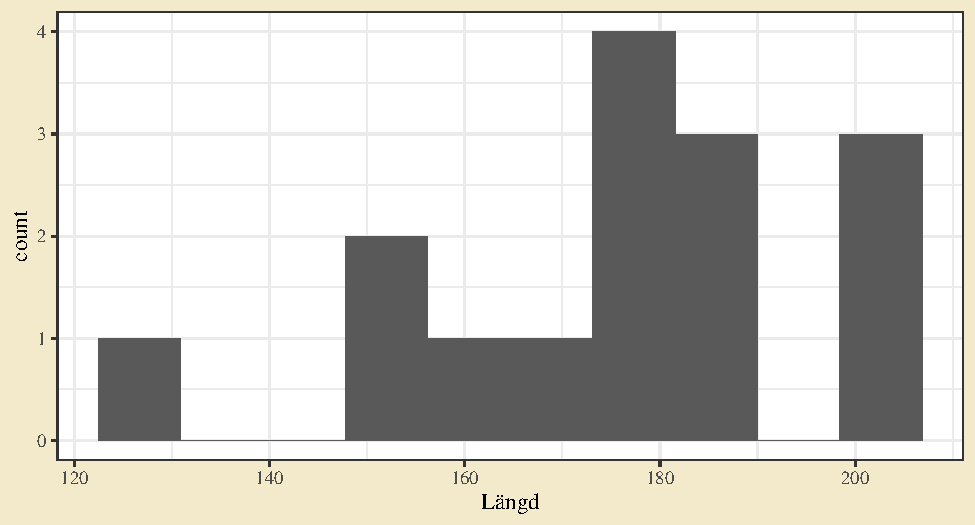
\includegraphics{R-anvisningar_files/figure-latex/unnamed-chunk-45-1} \end{center}

\begin{Shaded}
\begin{Highlighting}[]
\FunctionTok{ggplot}\NormalTok{(dat, }\FunctionTok{aes}\NormalTok{(Längd, }\StringTok{"Självbefruktning"}\NormalTok{)) }\SpecialCharTok{+} 
  \FunctionTok{geom\_boxplot}\NormalTok{() }\SpecialCharTok{+}
  \FunctionTok{ylab}\NormalTok{(}\StringTok{""}\NormalTok{)}
\end{Highlighting}
\end{Shaded}

\begin{center}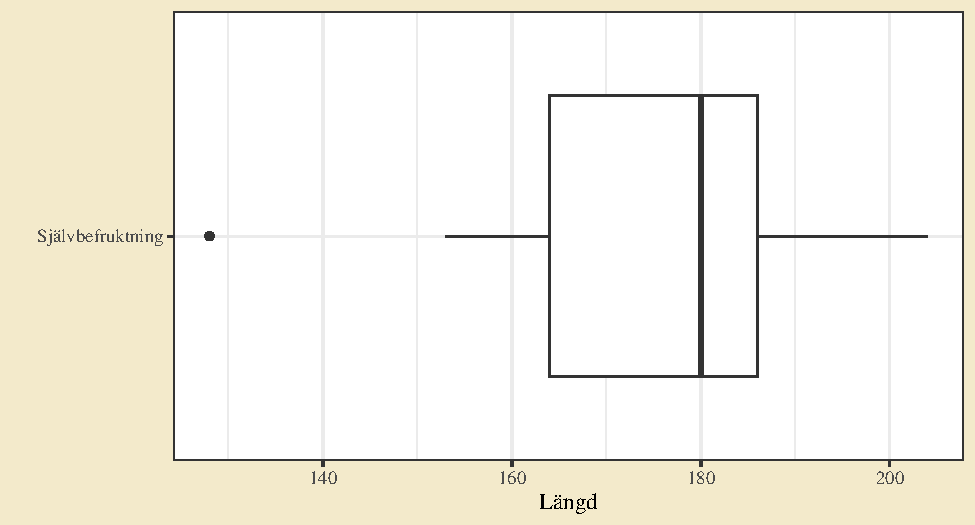
\includegraphics{R-anvisningar_files/figure-latex/unnamed-chunk-45-2} \end{center}

Storleken på intervallen i histogrammets x-axel kan styras med \texttt{binwidth}. Med så få observationer är histogram sällan informativt.
\end{hypothesis}

\begin{exercise}[Stapeldiagram med felstaplar]
Darwins studie gav följande data:

\begin{table}
\centering
\begin{tabular}[t]{rr}
\toprule
Självbefruktade & Korsbefruktade\\
\midrule
17.4 & 23.5\\
20.4 & 12.0\\
20.0 & 21.0\\
20.0 & 22.0\\
18.4 & 19.1\\
\addlinespace
18.6 & 21.5\\
18.6 & 22.1\\
15.3 & 20.4\\
16.5 & 18.3\\
18.0 & 21.6\\
\addlinespace
16.3 & 23.3\\
18.0 & 21.0\\
12.8 & 22.1\\
15.5 & 23.0\\
18.0 & 12.0\\
\bottomrule
\end{tabular}
\end{table}

Konstruera ett stapeldiagram med felstaplar där stapelns höjd ges av medelvärdet inom gruppen och felstapelns längd av standardavvikelsen inom gruppen.

Datan finns tillgänglig i arket \emph{Darwin} i excelfilen \emph{Uppgiftsdata.xlsx}. Exceldata kan läsas in med funktionen \texttt{read\_excel} från paketet \texttt{readxl}.
\end{exercise}

\begin{hypothesis}[Stapeldiagram med felstaplar]
Felstaplar kan konstrueras genom att beräkna medelvärde och standardavvikelse, och sedan \emph{pipa} (\texttt{\%\textgreater{}\%}) in i en plot där staplar konstrueras med \texttt{geom\_bar} och felstaplar med \texttt{geom\_errorbar}.

\begin{Shaded}
\begin{Highlighting}[]
\NormalTok{dat }\OtherTok{\textless{}{-}}\NormalTok{ readxl}\SpecialCharTok{::}\FunctionTok{read\_excel}\NormalTok{(}\StringTok{"Data/Uppgiftsdata.xlsx"}\NormalTok{, }\AttributeTok{sheet =} \StringTok{"Darwin"}\NormalTok{)}
\NormalTok{dat }\SpecialCharTok{\%\textgreater{}\%} 
  \FunctionTok{group\_by}\NormalTok{(Metod) }\SpecialCharTok{\%\textgreater{}\%} 
  \FunctionTok{summarise}\NormalTok{(}\AttributeTok{m =} \FunctionTok{mean}\NormalTok{(Utfall), }\AttributeTok{s =} \FunctionTok{sd}\NormalTok{(Utfall)) }\SpecialCharTok{\%\textgreater{}\%} 
  \FunctionTok{ggplot}\NormalTok{(}\FunctionTok{aes}\NormalTok{(Metod, m)) }\SpecialCharTok{+}
  \FunctionTok{geom\_bar}\NormalTok{(}\AttributeTok{stat =} \StringTok{"identity"}\NormalTok{, }\AttributeTok{width =} \FloatTok{0.3}\NormalTok{, }\AttributeTok{col =} \StringTok{"black"}\NormalTok{, }\AttributeTok{fill =} \StringTok{"white"}\NormalTok{) }\SpecialCharTok{+}
  \FunctionTok{geom\_errorbar}\NormalTok{(}\FunctionTok{aes}\NormalTok{(}\AttributeTok{ymin =}\NormalTok{ m }\SpecialCharTok{{-}}\NormalTok{ s, }\AttributeTok{ymax =}\NormalTok{ m }\SpecialCharTok{+}\NormalTok{ s), }\AttributeTok{width =} \FloatTok{0.1}\NormalTok{) }\SpecialCharTok{+}
  \FunctionTok{labs}\NormalTok{(}\AttributeTok{caption =} \StringTok{"Felstapel anger +/{-} en standardavvikelse"}\NormalTok{)}
\end{Highlighting}
\end{Shaded}

\begin{center}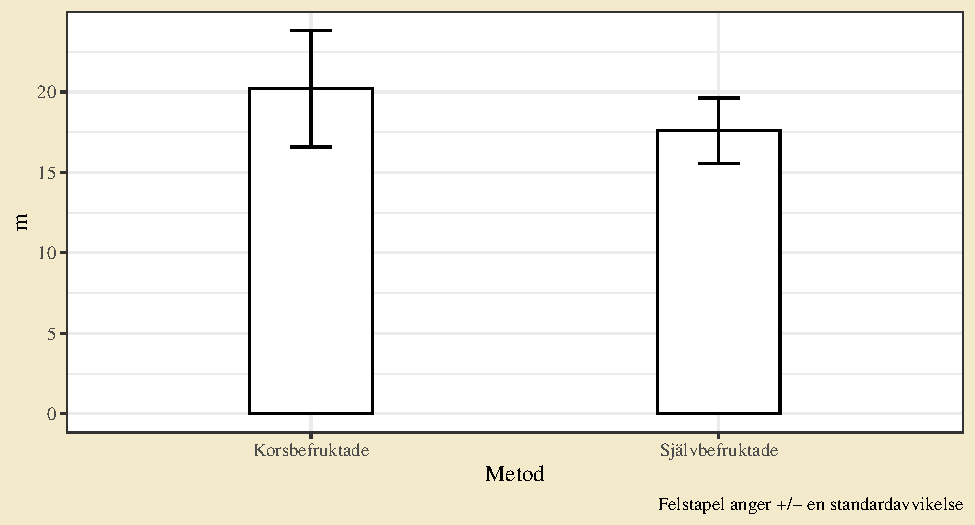
\includegraphics{R-anvisningar_files/figure-latex/unnamed-chunk-47-1} \end{center}

Det är inte alltid klart vilket spridningsmått felstaplarna illusterar (vanliga alternativ är standardavvikelsen, medelfelet (standardavvikelsen delat på roten ur stickprovsstorleken) och konfidensintervallet). Det är därför god praxis att skriva ut vad felstaplarna anger.
\end{hypothesis}

\begin{exercise}[Animal Crossing]
TidyTuesday (\url{https://github.com/rfordatascience/tidytuesday}) är ett R-kopplat projekt som varje vecka släpper ett nytt dataset, med tanken att vemsomhelst kan analysera datan och publicera informativa grafer. Ta gärna titt på Twitter under \emph{\#tidytuesday} (helst på en tisdag förstås). Ett dataset från TidyTuesday täcker bybor från spelserien \emph{Animal Crossing}. Datan kan läsas in med

\begin{Shaded}
\begin{Highlighting}[]
\NormalTok{villagers }\OtherTok{\textless{}{-}}\NormalTok{ readr}\SpecialCharTok{::}\FunctionTok{read\_csv}\NormalTok{(}\StringTok{\textquotesingle{}https://raw.githubusercontent.com/rfordatascience/tidytuesday/master/data/2020/2020{-}05{-}05/villagers.csv\textquotesingle{}}\NormalTok{)}
\end{Highlighting}
\end{Shaded}

a. Illustrera fördelning mellan arter (kolumnen \emph{species}) med ett lämpligt diagram. Försök att med hjälp av en internetsökning lösa de problem som kan uppstå med överlappande etiketter och ordning på staplar.

b. Utveckla diagrammet från (a) genom att på lämpligt sätt ange personlighet (kolumnen \emph{personality}).

c. Vilken är spelens mest populära låt?
\end{exercise}

\begin{hypothesis}[Animal Crossing]
a.

\begin{Shaded}
\begin{Highlighting}[]
\FunctionTok{ggplot}\NormalTok{(villagers, }\FunctionTok{aes}\NormalTok{(species)) }\SpecialCharTok{+}
  \FunctionTok{geom\_bar}\NormalTok{()}
\end{Highlighting}
\end{Shaded}

\begin{center}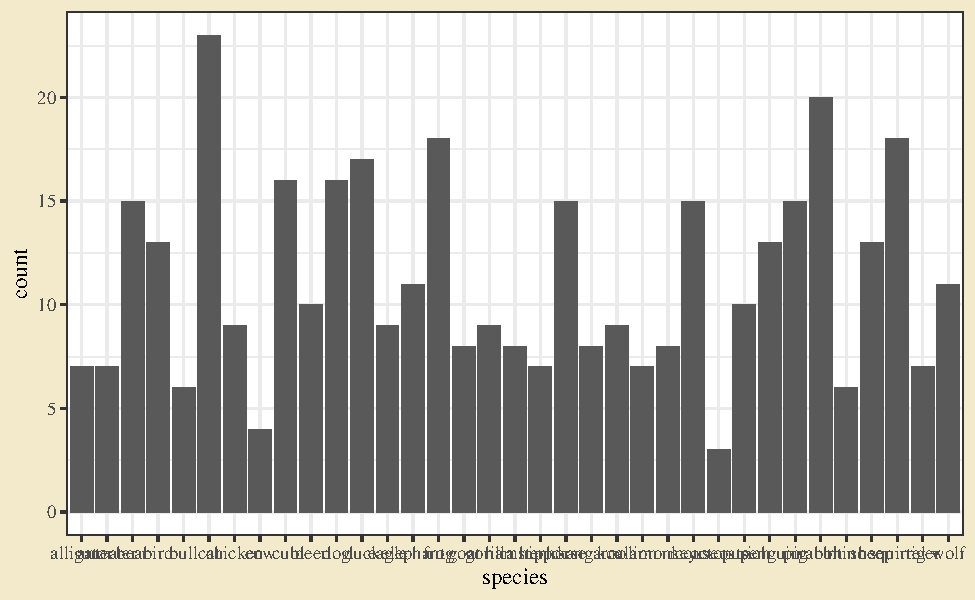
\includegraphics{R-anvisningar_files/figure-latex/unnamed-chunk-49-1} \end{center}

En internetsökning på exempelvis `ggplot2 bar order' kommer ge flera möjliga lösningar - en är att använda \texttt{fct\_reorder} från paketet \texttt{forcats}, vilket ordnar en faktor efter antalet förekomster (genom att sätta funktionen till \texttt{length}).
Överlappande etiketter kan också lösas på ett par olika sätt (lutande etiketter, etiketter på olika nivåer). En enkel lösning är att vrida staplarna och få etiketterna till vänster med \texttt{coord\_flip}.

\begin{Shaded}
\begin{Highlighting}[]
\FunctionTok{ggplot}\NormalTok{(villagers, }\FunctionTok{aes}\NormalTok{(forcats}\SpecialCharTok{::}\FunctionTok{fct\_reorder}\NormalTok{(species, species, }\AttributeTok{.fun =}\NormalTok{ length))) }\SpecialCharTok{+}
  \FunctionTok{geom\_bar}\NormalTok{() }\SpecialCharTok{+}
  \FunctionTok{xlab}\NormalTok{(}\StringTok{"Art"}\NormalTok{) }\SpecialCharTok{+}
  \FunctionTok{coord\_flip}\NormalTok{()}
\end{Highlighting}
\end{Shaded}

\begin{center}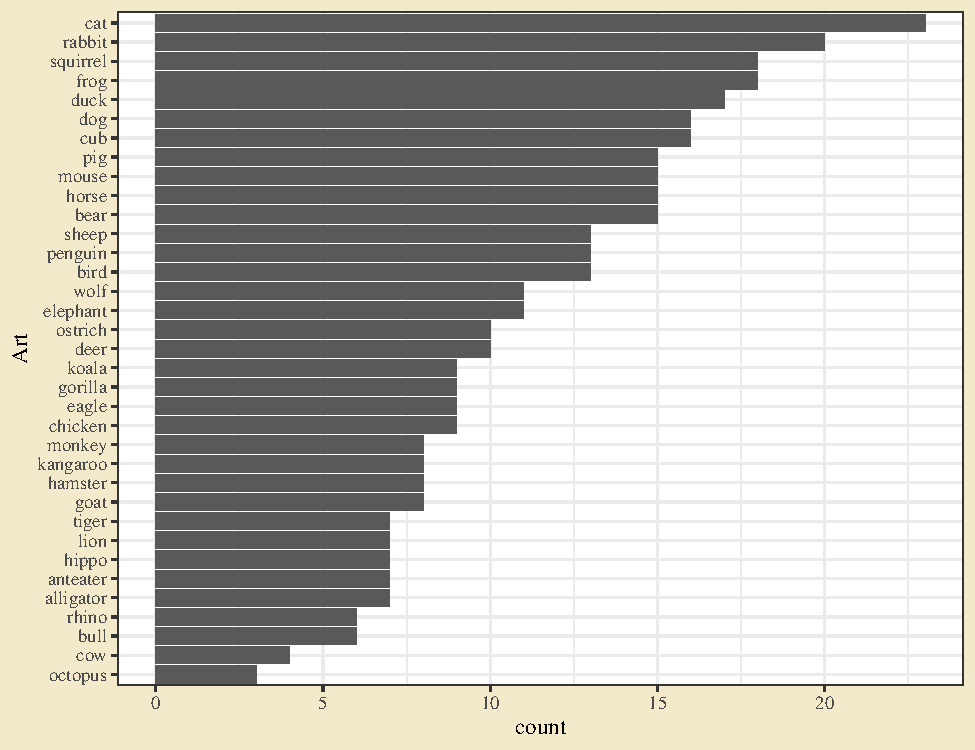
\includegraphics{R-anvisningar_files/figure-latex/unnamed-chunk-50-1} \end{center}

b.

\begin{Shaded}
\begin{Highlighting}[]
\FunctionTok{ggplot}\NormalTok{(villagers, }\FunctionTok{aes}\NormalTok{(forcats}\SpecialCharTok{::}\FunctionTok{fct\_reorder}\NormalTok{(species, species, }\AttributeTok{.fun =}\NormalTok{ length), }\AttributeTok{fill =}\NormalTok{ personality)) }\SpecialCharTok{+}
  \FunctionTok{geom\_bar}\NormalTok{() }\SpecialCharTok{+}
  \FunctionTok{xlab}\NormalTok{(}\StringTok{"Art"}\NormalTok{) }\SpecialCharTok{+}
  \FunctionTok{coord\_flip}\NormalTok{()}
\end{Highlighting}
\end{Shaded}

\begin{center}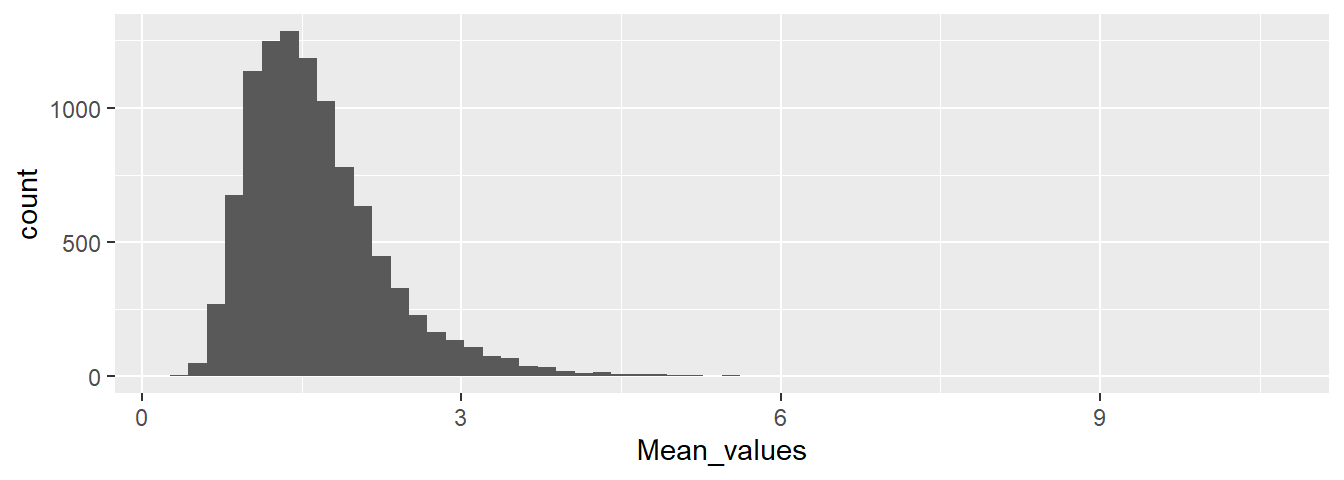
\includegraphics{R-anvisningar_files/figure-latex/unnamed-chunk-51-1} \end{center}

c.

\begin{Shaded}
\begin{Highlighting}[]
\NormalTok{villagers }\SpecialCharTok{\%\textgreater{}\%} 
  \FunctionTok{count}\NormalTok{(song, }\AttributeTok{sort =}\NormalTok{ T)}
\end{Highlighting}
\end{Shaded}

\begin{verbatim}
## # A tibble: 93 x 2
##    song              n
##    <chr>         <int>
##  1 <NA>             11
##  2 K.K. Country     10
##  3 Forest Life       9
##  4 I Love You        7
##  5 Imperial K.K.     7
##  6 K.K. Lament       7
##  7 K.K. Lullaby      7
##  8 K.K. Ragtime      7
##  9 K.K. Soul         7
## 10 Cafe K.K.         6
## # ... with 83 more rows
\end{verbatim}

Det vanligaste alternativet är att sång saknas, vilket då anges som \texttt{NA}. Den mest populära faktiska sången är \emph{KK Country}.
\end{hypothesis}

\begin{exercise}[Väderstation Falsterbo]
SMHI publicerar historisk väderdata från en stor mängd väderstationer (\url{https://www.smhi.se/data/meteorologi/ladda-ner-meteorologiska-observationer}). Ett exempel på en sådan fil, från väderstationen i Falsterbo, finns bland kursdatan. Notera att flera inledande rader innehåller metadata och inte ska läsas in. Filen är dessutom inte kommaseparerad utan semikolon-separerad. Den kan läsas in med funktionen \texttt{read\_csv2} från \texttt{readr}. Vid inläsning kan man också ändra datatyp för temperaturkolumnen, som annars felaktigt tolkats som en textkolumn.

\begin{Shaded}
\begin{Highlighting}[]
\NormalTok{dat }\OtherTok{\textless{}{-}} \FunctionTok{read\_csv2}\NormalTok{(}\StringTok{"Data/smhi{-}opendata\_1\_52230\_20210912\_114534.csv"}\NormalTok{, }\AttributeTok{skip =} \DecValTok{9}\NormalTok{) }\SpecialCharTok{\%\textgreater{}\%} 
  \FunctionTok{mutate}\NormalTok{(}\AttributeTok{Lufttemperatur =} \FunctionTok{as.numeric}\NormalTok{(Lufttemperatur))}
\end{Highlighting}
\end{Shaded}

a. Vilken är den högst uppmätta temperaturen?

b. Beräkna max-temperaturen för varje år. Plotta ett linjediagram med år på x-axeln och maxtemperatur på y-axeln.

c. Skapa en variabel som anger observationens årtionde. Beräkna medeltemperaturen per årtionde och illustrera med lämplig graf.
\end{exercise}

\begin{hypothesis}[Väderstation Falsterbo]
a. Ordna data efter lufttemperatur och skriv ut de översta raderna.

\begin{Shaded}
\begin{Highlighting}[]
\NormalTok{dat }\SpecialCharTok{\%\textgreater{}\%} \FunctionTok{arrange}\NormalTok{(}\FunctionTok{desc}\NormalTok{(Lufttemperatur)) }\SpecialCharTok{\%\textgreater{}\%} \FunctionTok{print}\NormalTok{(}\AttributeTok{n =} \DecValTok{10}\NormalTok{)}
\end{Highlighting}
\end{Shaded}

\begin{verbatim}
## # A tibble: 245,869 x 6
##    Datum      `Tid (UTC)` Lufttemperatur Kvalitet ...5  `Tidsutsnitt:`
##    <date>     <time>               <dbl> <chr>    <lgl> <chr>         
##  1 1994-07-31 12:00                 29.6 G        NA    <NA>          
##  2 1911-08-01 13:00                 28.8 G        NA    <NA>          
##  3 2018-08-03 15:00                 28.8 G        NA    <NA>          
##  4 2018-07-26 15:00                 28.7 G        NA    <NA>          
##  5 1994-07-28 12:00                 28.4 G        NA    <NA>          
##  6 2012-08-19 15:00                 28.4 G        NA    <NA>          
##  7 1994-07-28 15:00                 28.3 G        NA    <NA>          
##  8 2014-07-09 12:00                 28.2 G        NA    <NA>          
##  9 2018-08-02 15:00                 28.2 G        NA    <NA>          
## 10 2018-07-26 12:00                 28.1 G        NA    <NA>          
## # ... with 245,859 more rows
\end{verbatim}

Fem av de tio högsta mätningarna inträffade mellan 26 juli och 3 augusti 2018. Två samma dag.

b. Beräkningen kan göras genom att skapa en årsvariabel med \texttt{year} från \texttt{lubridate}-paketet. Därefter gruppera per år och summera med \texttt{max}-funktionen.

\begin{Shaded}
\begin{Highlighting}[]
\NormalTok{dat }\SpecialCharTok{\%\textgreater{}\%}
  \FunctionTok{mutate}\NormalTok{(Å}\AttributeTok{r =}\NormalTok{ lubridate}\SpecialCharTok{::}\FunctionTok{year}\NormalTok{(Datum)) }\SpecialCharTok{\%\textgreater{}\%} 
  \FunctionTok{group\_by}\NormalTok{(År) }\SpecialCharTok{\%\textgreater{}\%} 
  \FunctionTok{summarise}\NormalTok{(}\AttributeTok{Maxtemperatur =} \FunctionTok{max}\NormalTok{(Lufttemperatur)) }\SpecialCharTok{\%\textgreater{}\%} 
  \FunctionTok{ggplot}\NormalTok{(}\FunctionTok{aes}\NormalTok{(År, Maxtemperatur)) }\SpecialCharTok{+}
  \FunctionTok{geom\_line}\NormalTok{()}
\end{Highlighting}
\end{Shaded}

\begin{center}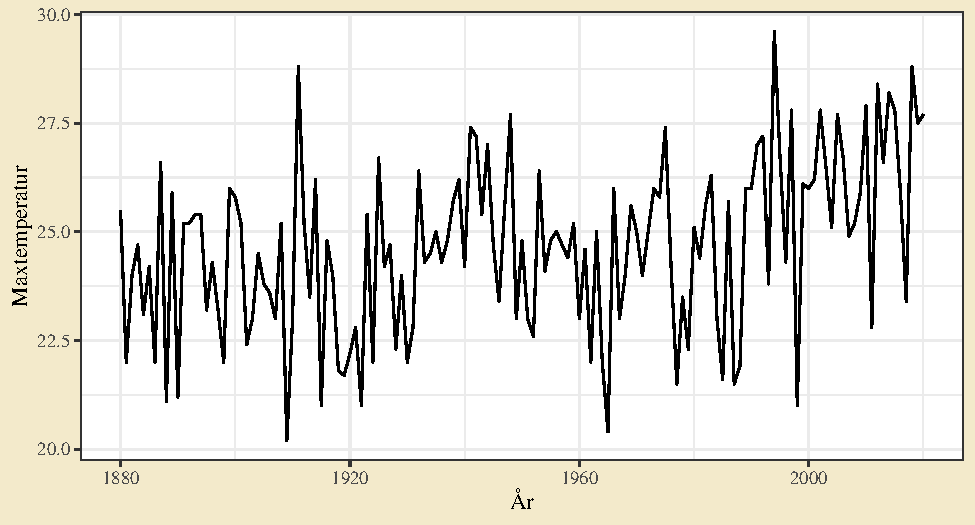
\includegraphics{R-anvisningar_files/figure-latex/unnamed-chunk-55-1} \end{center}

Datan visar på stor variation mellan år.

c. Likt (b) kan man skapa en årsvariabel och från den beräkna årtionde genom att dela på tio, använda \texttt{floor} för att ta bort decimalen, och sedan multiplicera med tio. Därefter kan man gruppera efter årtionde och summera till medelvärdet.

\begin{Shaded}
\begin{Highlighting}[]
\NormalTok{dat }\SpecialCharTok{\%\textgreater{}\%} 
  \FunctionTok{mutate}\NormalTok{(Å}\AttributeTok{rtionde =} \FunctionTok{floor}\NormalTok{(lubridate}\SpecialCharTok{::}\FunctionTok{year}\NormalTok{(Datum) }\SpecialCharTok{/} \DecValTok{10}\NormalTok{) }\SpecialCharTok{*} \DecValTok{10}\NormalTok{) }\SpecialCharTok{\%\textgreater{}\%} 
  \FunctionTok{group\_by}\NormalTok{(Årtionde) }\SpecialCharTok{\%\textgreater{}\%} 
  \FunctionTok{summarise}\NormalTok{(}\AttributeTok{Medeltemperatur =} \FunctionTok{mean}\NormalTok{(Lufttemperatur)) }\SpecialCharTok{\%\textgreater{}\%} 
  \FunctionTok{ggplot}\NormalTok{(}\FunctionTok{aes}\NormalTok{(Årtionde, Medeltemperatur, }\AttributeTok{fill =}\NormalTok{ Medeltemperatur)) }\SpecialCharTok{+}
  \FunctionTok{geom\_bar}\NormalTok{(}\AttributeTok{stat =} \StringTok{"identity"}\NormalTok{, }\AttributeTok{col =} \StringTok{"black"}\NormalTok{) }\SpecialCharTok{+}
  \FunctionTok{scale\_fill\_gradient}\NormalTok{(}\AttributeTok{low =} \StringTok{"yellow"}\NormalTok{, }\AttributeTok{high =} \StringTok{"red"}\NormalTok{)}
\end{Highlighting}
\end{Shaded}

\begin{center}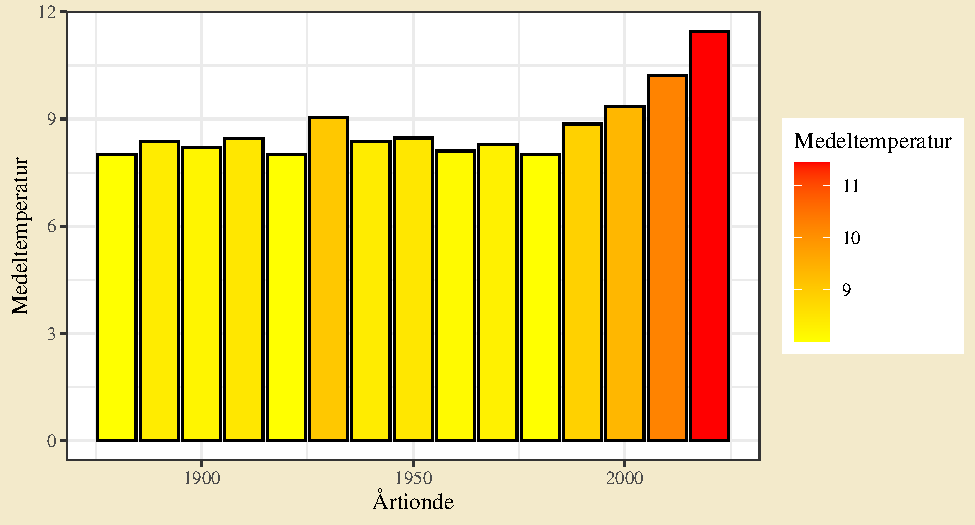
\includegraphics{R-anvisningar_files/figure-latex/unnamed-chunk-56-1} \end{center}

Temperaturen verkar öka i Falsterbo. Märk att stapeln för 2020-talet bara innefattar ett år.
\end{hypothesis}

\begin{exercise}[Allsvenskan för herrar]
Bland kursdatan finns en fil med matchresultat från herrarnas fotbollsallsvenska, 1924 - 2019. Läs in datan och undersök följande.

a. Hur många gånger har Malmö FF mött Mjällby? Vilket datum inföll Mjällbys enda seger?

b. Fyra säsonger har lag gått rent på hemmaplan (segrar i samtliga matcher). Vilka är de två lagen och vilka är de fyra säsongerna?

c. Vilka är de målrikaste matcherna?

d. Producera ett spridningsdiagram med hemmamål på x-axeln och bortamål på y-axeln. Hur kan man hantera överlappande punkter?
\end{exercise}

\begin{hypothesis}[Allsvenskan för herrar]
Filen kan läsas in med \texttt{read\_csv} från \texttt{readr}.

\begin{Shaded}
\begin{Highlighting}[]
\NormalTok{dat }\OtherTok{\textless{}{-}} \FunctionTok{read\_csv}\NormalTok{(}\StringTok{"Data/Allsvenskan, herrar, 1924{-}2019.csv"}\NormalTok{)}
\end{Highlighting}
\end{Shaded}

a. Matcher kan filtreras ut genom filter-funktionen. Två skilda rader kan användas för att få både hemma- och borta-matcher.

\begin{Shaded}
\begin{Highlighting}[]
\NormalTok{dat }\SpecialCharTok{\%\textgreater{}\%} \FunctionTok{filter}\NormalTok{(hemma }\SpecialCharTok{==} \StringTok{"Malmö FF"}\NormalTok{, borta }\SpecialCharTok{==} \StringTok{"Mjällby"}\NormalTok{)}
\end{Highlighting}
\end{Shaded}

\begin{verbatim}
## # A tibble: 8 x 6
##   datum      sasong hemma    borta   hemmamal bortamal
##   <date>     <chr>  <chr>    <chr>      <dbl>    <dbl>
## 1 1980-05-03 1980   Malmö FF Mjällby        1        0
## 2 1983-04-17 1983   Malmö FF Mjällby        1        1
## 3 1985-06-13 1985   Malmö FF Mjällby        2        0
## 4 2010-11-07 2010   Malmö FF Mjällby        2        0
## 5 2011-04-20 2011   Malmö FF Mjällby        1        0
## 6 2012-09-01 2012   Malmö FF Mjällby        1        1
## 7 2013-09-30 2013   Malmö FF Mjällby        1        0
## 8 2014-09-27 2014   Malmö FF Mjällby        4        1
\end{verbatim}

\begin{Shaded}
\begin{Highlighting}[]
\NormalTok{dat }\SpecialCharTok{\%\textgreater{}\%} \FunctionTok{filter}\NormalTok{(hemma }\SpecialCharTok{==} \StringTok{"Mjällby"}\NormalTok{, borta }\SpecialCharTok{==} \StringTok{"Malmö FF"}\NormalTok{)}
\end{Highlighting}
\end{Shaded}

\begin{verbatim}
## # A tibble: 8 x 6
##   datum      sasong hemma   borta    hemmamal bortamal
##   <date>     <chr>  <chr>   <chr>       <dbl>    <dbl>
## 1 1980-07-30 1980   Mjällby Malmö FF        1        1
## 2 1983-10-02 1983   Mjällby Malmö FF        1        1
## 3 1985-08-11 1985   Mjällby Malmö FF        1        1
## 4 2010-05-15 2010   Mjällby Malmö FF        4        2
## 5 2011-08-06 2011   Mjällby Malmö FF        1        1
## 6 2012-05-03 2012   Mjällby Malmö FF        2        2
## 7 2013-05-17 2013   Mjällby Malmö FF        2        2
## 8 2014-05-22 2014   Mjällby Malmö FF        0        1
\end{verbatim}

Lagen har mötts sexton gånger. Den enda malmöförlusten inträffade 2010 på bortaplan.

b. Andelen vinster på hemmaplan kan tas fram genom att gruppera på lag och säsong, beräkna antalet segrar och antalet matcher, och slutligen beräkna andelen segrar.
För att beräkna antalet vinster kan man använda \texttt{sum(hemmamal\ \textgreater{}\ bortamal)} - summan av antal gånger hemmamålen överstiger bortamålen. För det totala antalet matcher en säsong kan man använda funktionen \texttt{n()} - antalet rader i en viss gruppering.

\begin{Shaded}
\begin{Highlighting}[]
\NormalTok{dat }\SpecialCharTok{\%\textgreater{}\%} 
  \FunctionTok{group\_by}\NormalTok{(hemma, sasong) }\SpecialCharTok{\%\textgreater{}\%} 
  \FunctionTok{summarise}\NormalTok{(}\AttributeTok{Vinster =} \FunctionTok{sum}\NormalTok{(hemmamal }\SpecialCharTok{\textgreater{}}\NormalTok{ bortamal), }\AttributeTok{Total =} \FunctionTok{n}\NormalTok{()) }\SpecialCharTok{\%\textgreater{}\%} 
  \FunctionTok{mutate}\NormalTok{(}\AttributeTok{Proportion =}\NormalTok{ Vinster }\SpecialCharTok{/}\NormalTok{ Total) }\SpecialCharTok{\%\textgreater{}\%} 
  \FunctionTok{filter}\NormalTok{(Proportion }\SpecialCharTok{==} \DecValTok{1}\NormalTok{)}
\end{Highlighting}
\end{Shaded}

\begin{verbatim}
## # A tibble: 4 x 5
## # Groups:   hemma [2]
##   hemma        sasong    Vinster Total Proportion
##   <chr>        <chr>       <int> <int>      <dbl>
## 1 IFK Göteborg 1934_1935      11    11          1
## 2 IFK Göteborg 1941_1942      11    11          1
## 3 Malmö FF     1949_1950      11    11          1
## 4 Malmö FF     1950_1951      11    11          1
\end{verbatim}

Två lag (IFK Göteborg och Malmö FF) med två gånger var (1934-35 och 1941-42 respektive 1949-50 och 1950-51).

c. Skapa en ny variabel för totalt antal mål och sortera efter den kolumnen.

\begin{Shaded}
\begin{Highlighting}[]
\NormalTok{dat }\SpecialCharTok{\%\textgreater{}\%} 
  \FunctionTok{mutate}\NormalTok{(Mål }\OtherTok{=}\NormalTok{ hemmamal }\SpecialCharTok{+}\NormalTok{ bortamal) }\SpecialCharTok{\%\textgreater{}\%} 
  \FunctionTok{arrange}\NormalTok{(}\SpecialCharTok{{-}}\NormalTok{Mål) }\SpecialCharTok{\%\textgreater{}\%} 
  \FunctionTok{print}\NormalTok{(}\AttributeTok{n =} \DecValTok{5}\NormalTok{)}
\end{Highlighting}
\end{Shaded}

\begin{verbatim}
## # A tibble: 14,996 x 7
##   datum      sasong    hemma         borta      hemmamal bortamal   Mål
##   <date>     <chr>     <chr>         <chr>         <dbl>    <dbl> <dbl>
## 1 1928-10-21 1928_1929 Helsingborg   Eskilstuna       13        1    14
## 2 1936-04-19 1935_1936 Eskilstuna    Elfsborg          2       12    14
## 3 1954-11-06 1954_1955 Sandviken AIK AIK               4        9    13
## 4 1927-10-30 1927_1928 AIK           Eskilstuna        8        4    12
## 5 1928-11-04 1928_1929 Sleipner      Eskilstuna        7        5    12
## # ... with 14,991 more rows
\end{verbatim}

Två gånger har det blivit 14 mål. Bägge gångerna förluster för Eskilstuna.

d. Ett spridningsdiagram kan skapas med \texttt{ggplot}. Ett sätt att hantera överlappande punkter är att ge punkterna ett \emph{jitter} (ett slumpmässig justering så att de inte längre överlappar). Man kan också använda \texttt{geom\_count}, vilket gör att punktens storlek beror på antal överlappande observationer, eller skriva ut antalet överlappande fall.

\begin{Shaded}
\begin{Highlighting}[]
\NormalTok{g1 }\OtherTok{\textless{}{-}} \FunctionTok{ggplot}\NormalTok{(dat, }\FunctionTok{aes}\NormalTok{(hemmamal, bortamal)) }\SpecialCharTok{+}
  \FunctionTok{geom\_jitter}\NormalTok{(}\AttributeTok{size =} \FloatTok{0.1}\NormalTok{)}

\NormalTok{g2 }\OtherTok{\textless{}{-}} \FunctionTok{ggplot}\NormalTok{(dat, }\FunctionTok{aes}\NormalTok{(hemmamal, bortamal)) }\SpecialCharTok{+}
  \FunctionTok{geom\_count}\NormalTok{()}

\FunctionTok{library}\NormalTok{(patchwork)}
\NormalTok{g1 }\SpecialCharTok{+}\NormalTok{ g2}
\end{Highlighting}
\end{Shaded}

\begin{center}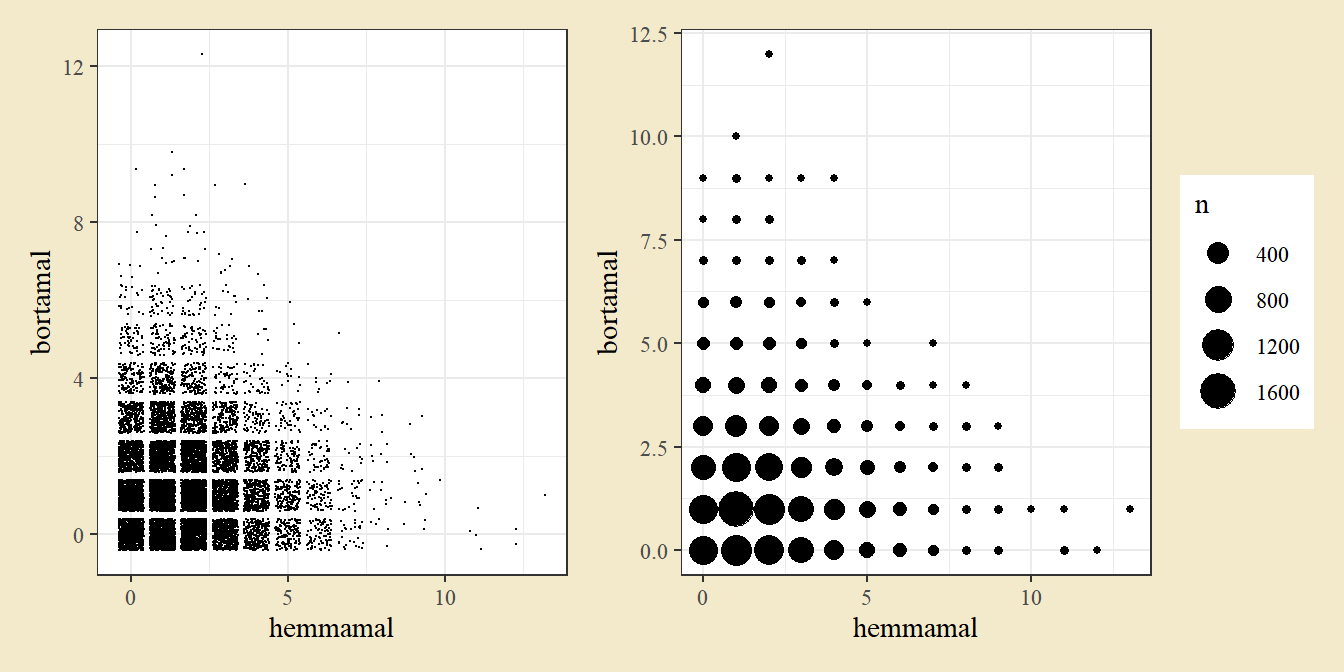
\includegraphics{R-anvisningar_files/figure-latex/unnamed-chunk-61-1} \end{center}

Det verkar som att 1-1 är det vanligaste resultatet. För att få en siffra kan man räkna hemma- och bortamål med \texttt{count}, för att sedan plotta med \texttt{geom\_text}.

\begin{Shaded}
\begin{Highlighting}[]
\NormalTok{dat }\SpecialCharTok{\%\textgreater{}\%} 
  \FunctionTok{count}\NormalTok{(hemmamal, bortamal) }\SpecialCharTok{\%\textgreater{}\%} 
  \FunctionTok{ggplot}\NormalTok{(}\FunctionTok{aes}\NormalTok{(hemmamal, bortamal, }\AttributeTok{label =}\NormalTok{ n)) }\SpecialCharTok{+}
  \FunctionTok{geom\_text}\NormalTok{(}\AttributeTok{size =} \DecValTok{3}\NormalTok{)}
\end{Highlighting}
\end{Shaded}

\begin{center}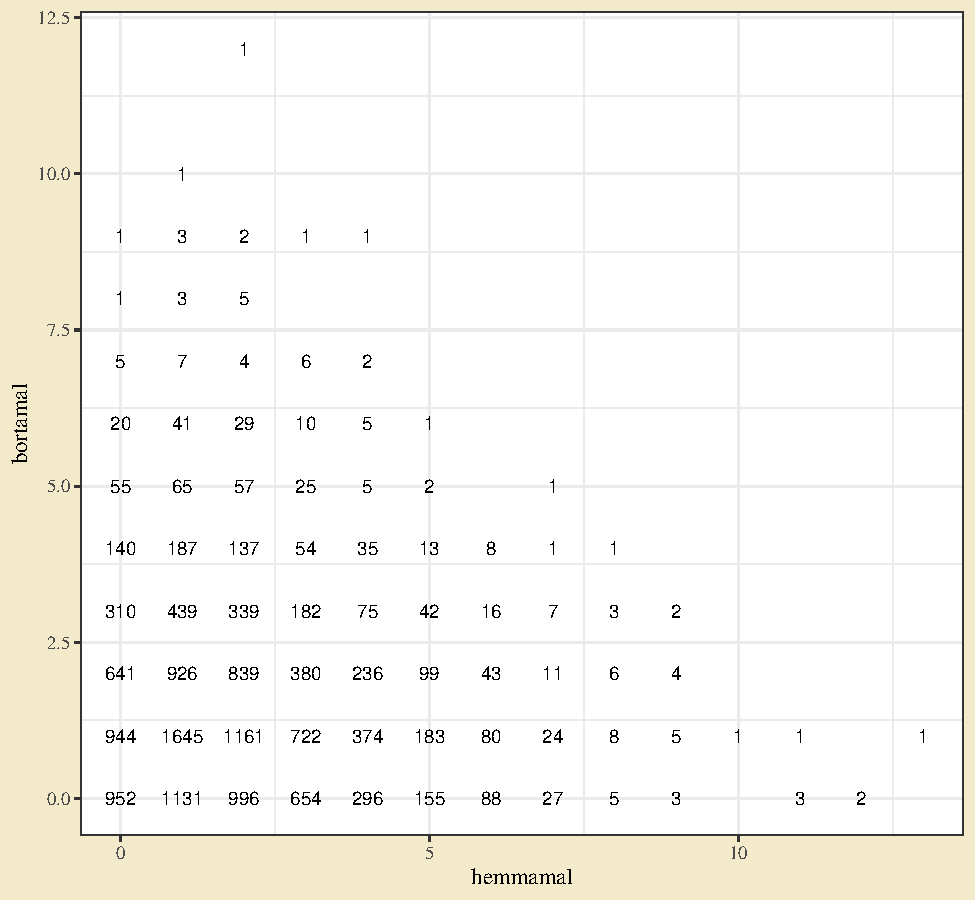
\includegraphics{R-anvisningar_files/figure-latex/unnamed-chunk-62-1} \end{center}

Det verkar som att 1-1, följt av 2-1 och 1-0 är de vanligaste resultaten.
\end{hypothesis}

\begin{exercise}[Egenskapad standardavvikelsefunktion]
En styrka med R är hur enkelt nya funktioner kan skapas. Många standardfunktioner är skrivna i R. Ta som exempel funktionen för standardavvikelse:

\begin{Shaded}
\begin{Highlighting}[]
\NormalTok{sd}
\end{Highlighting}
\end{Shaded}

\begin{verbatim}
## function (x, na.rm = FALSE) 
## sqrt(var(if (is.vector(x) || is.factor(x)) x else as.double(x), 
##     na.rm = na.rm))
## <bytecode: 0x0000000012339750>
## <environment: namespace:stats>
\end{verbatim}

Standardavvikelsen beräknas alltså som kvadratroten (\texttt{sqrt}) av variansen (\texttt{var}). Sedan finns också lite mer avancerad kod för att hantera olika typer av ingångsdata.

Standardavvikelsen av \(n\) datapunkter ges av

\[s = \sqrt{\frac{1}{n-1}\sum_{i=1}^n (x_i - \bar x)^2},\]

vilket kan brytas upp i steg som (1) beräkna medelvärdet, (2) dra ifrån medelvärdet från varje datavärde, (3) kvadrera differenserna, (4) summera kvadraterna, (5) dela summan med \(n-1\), och (6) ta kvadratroten ur kvoten.

Skapa en egen standardavvikelsefunktion baserat på de stegen. Funktionen ska ta en godtycklig mängd värden som ingångsvärden och ge standardavvikelsen som output.
\end{exercise}

\begin{hypothesis}[Egenskapad standardavvikelsefunktion]
Funktionen nedan går igenom stegen för att beräkna standardavvikelsen.

\begin{Shaded}
\begin{Highlighting}[]
\NormalTok{egen\_sd }\OtherTok{\textless{}{-}} \ControlFlowTok{function}\NormalTok{(x)\{}
\NormalTok{  n }\OtherTok{\textless{}{-}} \FunctionTok{length}\NormalTok{(x)          }\CommentTok{\# Spara datans storlek som n}
\NormalTok{  medel }\OtherTok{\textless{}{-}} \FunctionTok{mean}\NormalTok{(x)        }\CommentTok{\# 1}
\NormalTok{  diffs }\OtherTok{\textless{}{-}}\NormalTok{ x }\SpecialCharTok{{-}}\NormalTok{ medel      }\CommentTok{\# 2}
\NormalTok{  kvadrater }\OtherTok{\textless{}{-}}\NormalTok{ diffs}\SpecialCharTok{\^{}}\DecValTok{2}    \CommentTok{\# 3}
\NormalTok{  summa }\OtherTok{\textless{}{-}} \FunctionTok{sum}\NormalTok{(kvadrater) }\CommentTok{\# 4}
\NormalTok{  kvot }\OtherTok{\textless{}{-}}\NormalTok{ summa }\SpecialCharTok{/}\NormalTok{ (n }\SpecialCharTok{{-}} \DecValTok{1}\NormalTok{) }\CommentTok{\# 5}
\NormalTok{  s }\OtherTok{\textless{}{-}} \FunctionTok{sqrt}\NormalTok{(kvot)         }\CommentTok{\# 6}
\NormalTok{  s                       }\CommentTok{\# Ange output}
\NormalTok{\}}

\NormalTok{dat }\OtherTok{\textless{}{-}} \FunctionTok{c}\NormalTok{(}\DecValTok{3}\NormalTok{,}\DecValTok{1}\NormalTok{,}\DecValTok{4}\NormalTok{,}\DecValTok{5}\NormalTok{,}\DecValTok{9}\NormalTok{)}
\FunctionTok{sd}\NormalTok{(dat)}
\end{Highlighting}
\end{Shaded}

\begin{verbatim}
## [1] 2.966479
\end{verbatim}

\begin{Shaded}
\begin{Highlighting}[]
\FunctionTok{egen\_sd}\NormalTok{(dat)}
\end{Highlighting}
\end{Shaded}

\begin{verbatim}
## [1] 2.966479
\end{verbatim}

Den egenskapade funktionen ger samma utfall som R funktionen \texttt{sd}.
\end{hypothesis}

\hypertarget{sannolikhetsfuxf6rdelningar-och-slumptal}{%
\chapter{Sannolikhetsfördelningar och slumptal}\label{sannolikhetsfuxf6rdelningar-och-slumptal}}

\hypertarget{fuxf6rdelningar}{%
\section{Fördelningar}\label{fuxf6rdelningar}}

R kommer med en stor mängd funktioner för att beräkna sannolikheter ur kända sannolikhetsfördelningar såsom binomial- och normalfördelningen. För en lista på fördelningar täckta av grundpaketen i R kan man köra \texttt{?distributions}.

För en \emph{kontinuerlig likformig fördelning} gäller att alla utfall mellan 0 och 1 är lika sannolika. Som exempel kan man tänka sig att man stoppar ett tidtagarur vid ett slumpmässigt tillfälle och tittar på utfallets decimaler - de kommer ge ett värde mellan 0 och 1 och det finns ingen anledning att tro att vissa värden är mer sannolika än andra. Täthetsfunktionen \(f(x)\) kan beräknas genom \(dunif\), där \texttt{d} står för \emph{density} (täthet) och \texttt{unif} anger en \emph{uniform} fördelning. Fördelningens täthetsfunktion är 0 för värden på \(x\) under 0 eller över 1, och däremellan är täthetsfunktionen 1.

\begin{Shaded}
\begin{Highlighting}[]
\FunctionTok{dunif}\NormalTok{(}\SpecialCharTok{{-}}\FloatTok{0.1}\NormalTok{)}
\end{Highlighting}
\end{Shaded}

\begin{verbatim}
## [1] 0
\end{verbatim}

\begin{Shaded}
\begin{Highlighting}[]
\FunctionTok{dunif}\NormalTok{(}\FloatTok{0.1}\NormalTok{)}
\end{Highlighting}
\end{Shaded}

\begin{verbatim}
## [1] 1
\end{verbatim}

\begin{Shaded}
\begin{Highlighting}[]
\FunctionTok{dunif}\NormalTok{(}\FloatTok{1.1}\NormalTok{)}
\end{Highlighting}
\end{Shaded}

\begin{verbatim}
## [1] 0
\end{verbatim}

Fördelningsfunktionen anger sannolikheten för ett värde mindre än \(x\), \(F(x) = P(X \leq x)\) och kan i R beräknas genom funktionen \(punif\), där \texttt{p} står för \emph{probability}.

\begin{Shaded}
\begin{Highlighting}[]
\FunctionTok{punif}\NormalTok{(}\SpecialCharTok{{-}}\FloatTok{0.1}\NormalTok{)}
\end{Highlighting}
\end{Shaded}

\begin{verbatim}
## [1] 0
\end{verbatim}

\begin{Shaded}
\begin{Highlighting}[]
\FunctionTok{punif}\NormalTok{(}\FloatTok{0.1}\NormalTok{)}
\end{Highlighting}
\end{Shaded}

\begin{verbatim}
## [1] 0.1
\end{verbatim}

\begin{Shaded}
\begin{Highlighting}[]
\FunctionTok{punif}\NormalTok{(}\FloatTok{1.1}\NormalTok{)}
\end{Highlighting}
\end{Shaded}

\begin{verbatim}
## [1] 1
\end{verbatim}

Fördelningsfunktionen för en likformig fördelning är för värden på \(x\) under 0, 1 för värden på \(x\) över 1, och däremellan lika med \(x\).

Täthetsfunktion och fördelningsfunktion kan illustreras med grafer. Funktionen \texttt{seq} används för att skapa en sekvens från ett värde till ett annat värde. Paketet \texttt{patchwork} används för att kombinera två grafer. Funktionen \texttt{tibble} används för att skapa ett \texttt{tibble}-objekt - funktionen fungerar likt \texttt{data.frame} i att kolumner anges som \texttt{namn\ =\ kolumnvärden}.

\begin{Shaded}
\begin{Highlighting}[]
\NormalTok{g1 }\OtherTok{\textless{}{-}} \FunctionTok{tibble}\NormalTok{(}\AttributeTok{x =} \FunctionTok{seq}\NormalTok{(}\AttributeTok{from =} \SpecialCharTok{{-}}\FloatTok{0.5}\NormalTok{, }\AttributeTok{to =} \FloatTok{1.5}\NormalTok{, }\AttributeTok{by =} \FloatTok{0.01}\NormalTok{),}
             \AttributeTok{f =} \FunctionTok{dunif}\NormalTok{(x)) }\SpecialCharTok{\%\textgreater{}\%} 
  \FunctionTok{ggplot}\NormalTok{(}\FunctionTok{aes}\NormalTok{(x, f)) }\SpecialCharTok{+} 
  \FunctionTok{geom\_line}\NormalTok{() }\SpecialCharTok{+}
  \FunctionTok{labs}\NormalTok{(}\AttributeTok{title =} \StringTok{"Täthetsfunktion, f(x)"}\NormalTok{)}

\NormalTok{g2 }\OtherTok{\textless{}{-}} \FunctionTok{tibble}\NormalTok{(}\AttributeTok{x =} \FunctionTok{seq}\NormalTok{(}\AttributeTok{from =} \SpecialCharTok{{-}}\FloatTok{0.5}\NormalTok{, }\AttributeTok{to =} \FloatTok{1.5}\NormalTok{, }\AttributeTok{by =} \FloatTok{0.01}\NormalTok{),}
             \AttributeTok{F =} \FunctionTok{punif}\NormalTok{(x)) }\SpecialCharTok{\%\textgreater{}\%} 
  \FunctionTok{ggplot}\NormalTok{(}\FunctionTok{aes}\NormalTok{(x, F)) }\SpecialCharTok{+} 
  \FunctionTok{geom\_line}\NormalTok{() }\SpecialCharTok{+}
  \FunctionTok{labs}\NormalTok{(}\AttributeTok{title =} \StringTok{"Fördelningsfunktion, F(x)"}\NormalTok{)}

\FunctionTok{library}\NormalTok{(patchwork)}
\NormalTok{g1 }\SpecialCharTok{+}\NormalTok{ g2}
\end{Highlighting}
\end{Shaded}

\begin{center}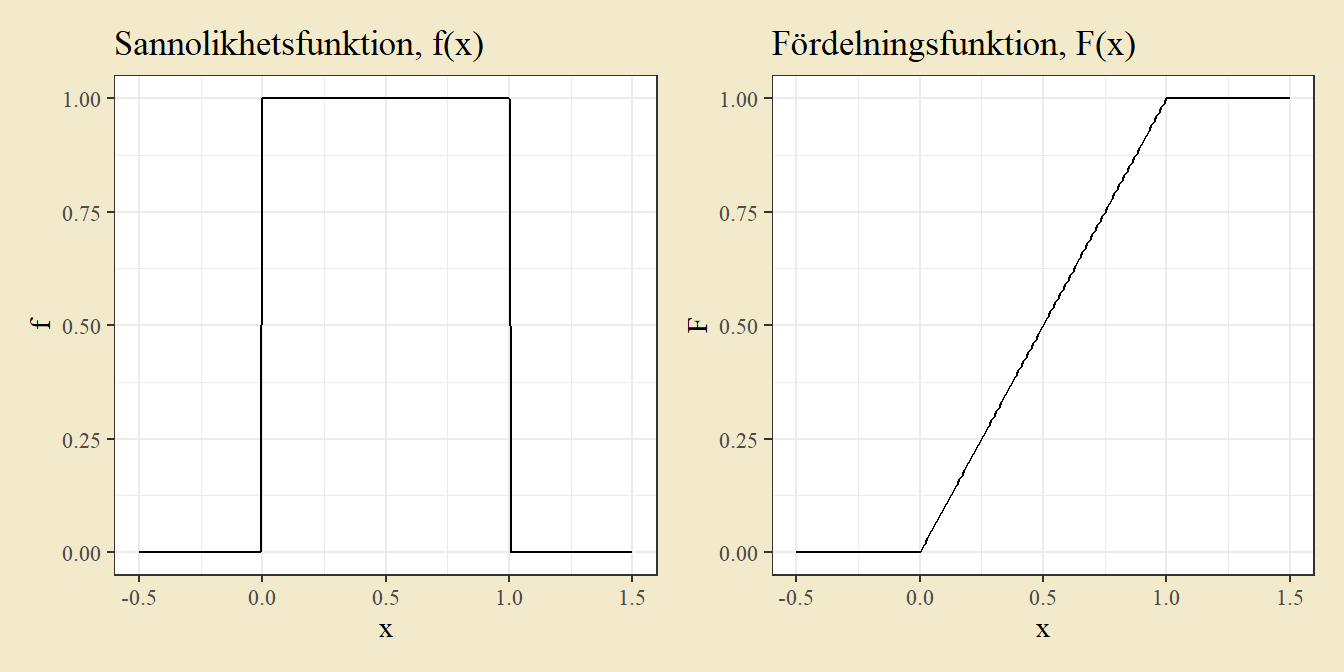
\includegraphics{R-anvisningar_files/figure-latex/unnamed-chunk-66-1} \end{center}

Motsvarande funktioner för en normalfördelning ges av \texttt{dnorm} och \texttt{pnorm}. Medelvärde och standardavvikelse kan sättas genom argumenten \texttt{mean} och \texttt{sd}. Här ges ett exempel på en normalfördelning med medelvärdet 50 och standardavvikelse 3.

\begin{Shaded}
\begin{Highlighting}[]
\NormalTok{g1 }\OtherTok{\textless{}{-}} \FunctionTok{tibble}\NormalTok{(}\AttributeTok{x =} \FunctionTok{seq}\NormalTok{(}\AttributeTok{from =} \DecValTok{40}\NormalTok{, }\AttributeTok{to =} \DecValTok{60}\NormalTok{, }\AttributeTok{by =} \FloatTok{0.1}\NormalTok{),}
             \AttributeTok{f =} \FunctionTok{dnorm}\NormalTok{(x, }\AttributeTok{mean =} \DecValTok{50}\NormalTok{, }\AttributeTok{sd =} \DecValTok{3}\NormalTok{)) }\SpecialCharTok{\%\textgreater{}\%} 
  \FunctionTok{ggplot}\NormalTok{(}\FunctionTok{aes}\NormalTok{(x, f)) }\SpecialCharTok{+} 
  \FunctionTok{geom\_line}\NormalTok{() }\SpecialCharTok{+}
  \FunctionTok{labs}\NormalTok{(}\AttributeTok{title =} \StringTok{"Täthetsfunktion, f(x)"}\NormalTok{)}

\NormalTok{g2 }\OtherTok{\textless{}{-}} \FunctionTok{tibble}\NormalTok{(}\AttributeTok{x =} \FunctionTok{seq}\NormalTok{(}\AttributeTok{from =} \DecValTok{40}\NormalTok{, }\AttributeTok{to =} \DecValTok{60}\NormalTok{, }\AttributeTok{by =} \FloatTok{0.1}\NormalTok{),}
             \AttributeTok{F =} \FunctionTok{pnorm}\NormalTok{(x, }\AttributeTok{mean =} \DecValTok{50}\NormalTok{, }\AttributeTok{sd =} \DecValTok{3}\NormalTok{)) }\SpecialCharTok{\%\textgreater{}\%} 
  \FunctionTok{ggplot}\NormalTok{(}\FunctionTok{aes}\NormalTok{(x, F)) }\SpecialCharTok{+} 
  \FunctionTok{geom\_line}\NormalTok{() }\SpecialCharTok{+}
  \FunctionTok{labs}\NormalTok{(}\AttributeTok{title =} \StringTok{"Fördelningsfunktion, F(x)"}\NormalTok{)}

\NormalTok{g1 }\SpecialCharTok{+}\NormalTok{ g2}
\end{Highlighting}
\end{Shaded}

\begin{center}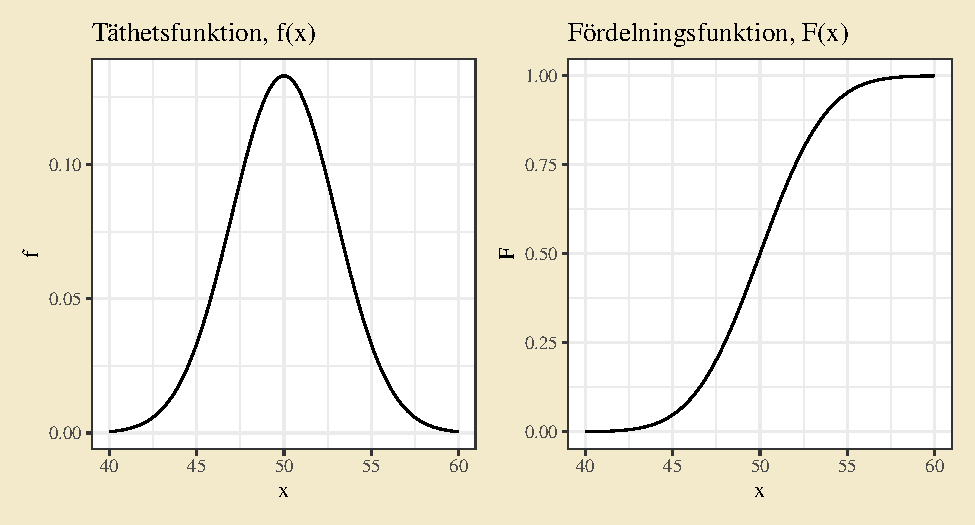
\includegraphics{R-anvisningar_files/figure-latex/unnamed-chunk-67-1} \end{center}

Fördelningsfunktionen anger sannolikheten att ett utfall ligger under värdet \(x\). Om man vill beräkna det omvända fallet - ett x-värde sådant att sannolikheten att ligga under det värdet är en viss sannolikhet \(p\) - använder man \emph{kvantilfunktionen}. Som exempel beräknas ett värde på x-axeln sådant att en fjärdedel ligger under det värdet i en normalfördelning med \(\mu = 50\) och \(\sigma = 3\).

\begin{Shaded}
\begin{Highlighting}[]
\FunctionTok{qnorm}\NormalTok{(}\FloatTok{0.25}\NormalTok{, }\AttributeTok{mean =} \DecValTok{50}\NormalTok{, }\AttributeTok{sd =} \DecValTok{3}\NormalTok{)}
\end{Highlighting}
\end{Shaded}

\begin{verbatim}
## [1] 47.97653
\end{verbatim}

Sannolikhetsfunktion och fördelningsfunktion kan även beräknas för diskreta fördelningar. Binomialfördelningen ges till exempel av \texttt{dbinom} och \texttt{pbinom} med argumenten \texttt{size} för parametern \(n\) och \texttt{prob} för parametern \(p\). Här ges ett exempel på en binomialfördelning med \(n = 20\) och \(p = 0.7\). Eftersom en diskret fördelning oftast illustreras med stapeldiagram ersätts \texttt{geom\_line()} med \texttt{geom\_bar(stat\ =\ "identity")}.

\begin{Shaded}
\begin{Highlighting}[]
\NormalTok{g1 }\OtherTok{\textless{}{-}} \FunctionTok{tibble}\NormalTok{(}\AttributeTok{x =} \DecValTok{0}\SpecialCharTok{:}\DecValTok{20}\NormalTok{,}
             \AttributeTok{f =} \FunctionTok{dbinom}\NormalTok{(x, }\AttributeTok{size =} \DecValTok{20}\NormalTok{, }\AttributeTok{prob =} \FloatTok{0.7}\NormalTok{)) }\SpecialCharTok{\%\textgreater{}\%} 
  \FunctionTok{ggplot}\NormalTok{(}\FunctionTok{aes}\NormalTok{(x, f)) }\SpecialCharTok{+} 
  \FunctionTok{geom\_bar}\NormalTok{(}\AttributeTok{stat =} \StringTok{"identity"}\NormalTok{) }\SpecialCharTok{+}
  \FunctionTok{labs}\NormalTok{(}\AttributeTok{title =} \StringTok{"Sannolikhetsfunktion, f(x)"}\NormalTok{)}

\NormalTok{g2 }\OtherTok{\textless{}{-}} \FunctionTok{tibble}\NormalTok{(}\AttributeTok{x =} \DecValTok{0}\SpecialCharTok{:}\DecValTok{20}\NormalTok{,}
             \AttributeTok{F =} \FunctionTok{pbinom}\NormalTok{(x, }\AttributeTok{size =} \DecValTok{20}\NormalTok{, }\AttributeTok{prob =} \FloatTok{0.7}\NormalTok{)) }\SpecialCharTok{\%\textgreater{}\%} 
  \FunctionTok{ggplot}\NormalTok{(}\FunctionTok{aes}\NormalTok{(x, F)) }\SpecialCharTok{+} 
  \FunctionTok{geom\_bar}\NormalTok{(}\AttributeTok{stat =} \StringTok{"identity"}\NormalTok{) }\SpecialCharTok{+}
  \FunctionTok{labs}\NormalTok{(}\AttributeTok{title =} \StringTok{"Fördelningsfunktion, F(x)"}\NormalTok{)}

\NormalTok{g1 }\SpecialCharTok{+}\NormalTok{ g2}
\end{Highlighting}
\end{Shaded}

\begin{center}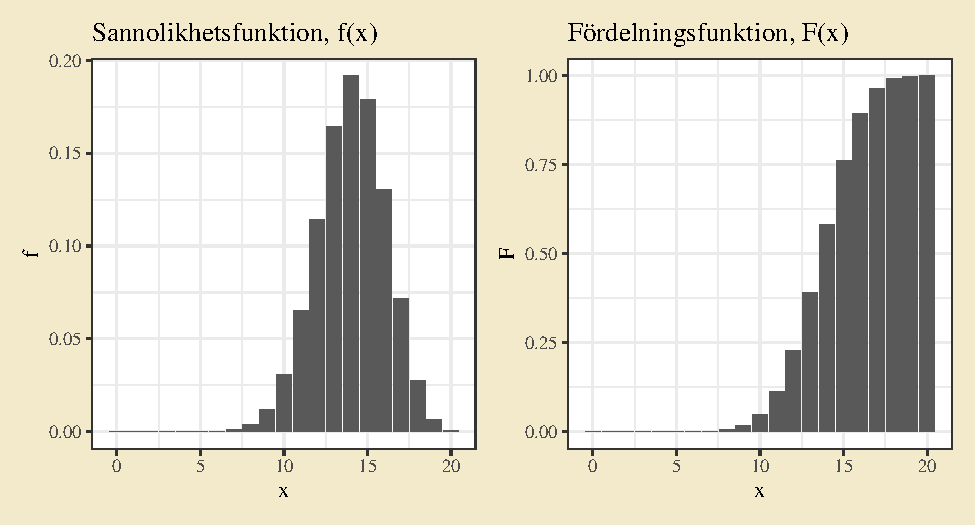
\includegraphics{R-anvisningar_files/figure-latex/unnamed-chunk-69-1} \end{center}

Utöver sannolikhetsberäkningar har R funktioner för att skapa slumptal från en angiven fördelning. Dessa anges genom bokstaven \texttt{r} (för \emph{random}) följt av fördelningens namn, t.ex. \texttt{rnorm} för normalfördelningen och \texttt{rbinom} för binomialfördelningen. I exemplet nedan dras tiotusen observationer från en normalfördelning. Histogrammet visar att slumptalen ungefär följer den teoretiska fördelningen (här utritad med funktionen \texttt{stat\_function}).

\begin{Shaded}
\begin{Highlighting}[]
\NormalTok{dat }\OtherTok{\textless{}{-}} \FunctionTok{tibble}\NormalTok{(}\AttributeTok{x =} \FunctionTok{rnorm}\NormalTok{(}\DecValTok{10000}\NormalTok{, }\AttributeTok{mean =} \DecValTok{50}\NormalTok{, }\AttributeTok{sd =} \DecValTok{3}\NormalTok{))}
\FunctionTok{ggplot}\NormalTok{(dat, }\FunctionTok{aes}\NormalTok{(x)) }\SpecialCharTok{+}
  \FunctionTok{geom\_histogram}\NormalTok{(}\FunctionTok{aes}\NormalTok{(}\AttributeTok{y =}\NormalTok{..density..)) }\SpecialCharTok{+}
  \FunctionTok{stat\_function}\NormalTok{(}\AttributeTok{fun =}\NormalTok{ dnorm, }\AttributeTok{args =} \FunctionTok{list}\NormalTok{(}\AttributeTok{mean =} \DecValTok{50}\NormalTok{, }\AttributeTok{sd =} \DecValTok{3}\NormalTok{), }
                \AttributeTok{col =} \StringTok{"red"}\NormalTok{, }\AttributeTok{size =} \DecValTok{1}\NormalTok{)}
\end{Highlighting}
\end{Shaded}

\begin{center}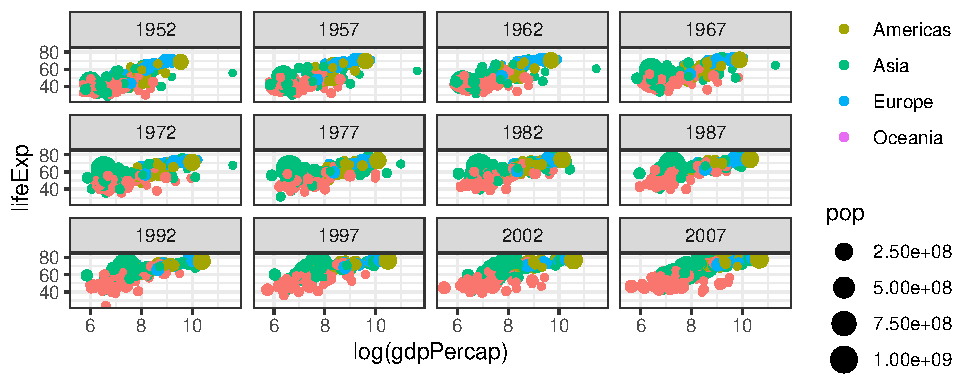
\includegraphics{R-anvisningar_files/figure-latex/unnamed-chunk-70-1} \end{center}

Argumentet \texttt{y\ =\ ..density..} anger att y-axeln ska vara i andelar, istället för antal.

\hypertarget{egna-funktioner}{%
\section{Egna funktioner}\label{egna-funktioner}}

Det är möjligt att definera egna funktioner genom konstruktionsfunktionen \texttt{function}. Ett enkelt exempel på en funktion som tar ett värde och ger det värdet plus 4:

\begin{Shaded}
\begin{Highlighting}[]
\NormalTok{add\_four }\OtherTok{\textless{}{-}} \ControlFlowTok{function}\NormalTok{(x)\{}
\NormalTok{  y }\OtherTok{\textless{}{-}}\NormalTok{ x }\SpecialCharTok{+} \DecValTok{4}
\NormalTok{  y}
\NormalTok{\}}

\FunctionTok{add\_four}\NormalTok{(}\DecValTok{5}\NormalTok{)}
\end{Highlighting}
\end{Shaded}

\begin{verbatim}
## [1] 9
\end{verbatim}

Här är \texttt{add\_four} namnet på den funktion som skapas och \texttt{function(x)} anger att man skapar en funktion med ett ingångsvärde \texttt{x}. Stycket inom \texttt{\{...\}} är själva funktionsberäkning. I det här fallet skapar funktionen ett objekt \texttt{y} som ges av x plus 4, och därefter skrivs resultatet ut. Det som skrivs ut i funktionens sista rad blir funktionens output.

Funktioner kan ha mer än ett ingående värde, t.ex.

\begin{Shaded}
\begin{Highlighting}[]
\NormalTok{add\_two\_numbers }\OtherTok{\textless{}{-}} \ControlFlowTok{function}\NormalTok{(x, y)\{}
\NormalTok{  res }\OtherTok{\textless{}{-}}\NormalTok{ x }\SpecialCharTok{+}\NormalTok{ y}
\NormalTok{  res}
\NormalTok{\}}

\FunctionTok{add\_two\_numbers}\NormalTok{(}\DecValTok{15}\NormalTok{, }\DecValTok{3}\NormalTok{)}
\end{Highlighting}
\end{Shaded}

\begin{verbatim}
## [1] 18
\end{verbatim}

Ett ingångsvärde kan ges ett grundläge genom att ange det som ett argument i funktionen, t.ex.

\begin{Shaded}
\begin{Highlighting}[]
\NormalTok{add\_two\_numbers }\OtherTok{\textless{}{-}} \ControlFlowTok{function}\NormalTok{(x, }\AttributeTok{y =} \DecValTok{3}\NormalTok{)\{}
\NormalTok{  res }\OtherTok{\textless{}{-}}\NormalTok{ x }\SpecialCharTok{+}\NormalTok{ y}
\NormalTok{  res}
\NormalTok{\}}

\FunctionTok{add\_two\_numbers}\NormalTok{(}\DecValTok{15}\NormalTok{)}
\end{Highlighting}
\end{Shaded}

\begin{verbatim}
## [1] 18
\end{verbatim}

\begin{Shaded}
\begin{Highlighting}[]
\FunctionTok{add\_two\_numbers}\NormalTok{(}\DecValTok{15}\NormalTok{, }\DecValTok{12}\NormalTok{)}
\end{Highlighting}
\end{Shaded}

\begin{verbatim}
## [1] 27
\end{verbatim}

Om inget värde anges för det andra ingåendevärdet (y) sätts det värdet till 3, eftersom det anges i definitionen av funktionen.

\hypertarget{simuleringar}{%
\section{Simuleringar}\label{simuleringar}}

Med hjälp av egna funktioner och slumptal kan man utforska många grundläggande statistiska resultat. Teoretiska resultat säger till exempel att om en slumpvariabel \(X\) har standardavvikelsen \(\sigma\), så har ett medelvärde av \(n\) observationer av \(X\) standardavvikelsen \(\sigma / \sqrt n\). För att undersöka detta skapas en funktion som för ett angivet värde på \(n\) ger ett medelvärde av \(n\) slumptal.

\begin{Shaded}
\begin{Highlighting}[]
\NormalTok{mean\_of\_n\_obs }\OtherTok{\textless{}{-}} \ControlFlowTok{function}\NormalTok{(}\AttributeTok{n =} \DecValTok{1}\NormalTok{)\{}
\NormalTok{  x }\OtherTok{\textless{}{-}} \FunctionTok{rnorm}\NormalTok{(n, }\AttributeTok{mean =} \DecValTok{0}\NormalTok{, }\AttributeTok{sd =} \DecValTok{1}\NormalTok{)}
  \FunctionTok{mean}\NormalTok{(x)}
\NormalTok{\}}
\end{Highlighting}
\end{Shaded}

Funktionen tar ingångsvärdet n, simulerar n stycken slumptal från en normalfördelning med medelvärde 0 och standardavvikelse 1, och ger ut medelvärdet av de slumptalen.

Funktionen \texttt{replicate} kan användas för att köra en funktion upprepade gånger - \texttt{replicate(100,\ mean\_of\_n\_obs(n\ =\ 10))} upprepar den definerade funktionen 100 gånger och ger alltså 100 stycken medelvärden där varje medelvärde beräknas från 10 observationer.

Eftersom standardavvikelsen i den ursprungliga dragningen var 1 (\(\sigma = 1\)) bör standardavvikelsen i ett medelvärde av 16 observationer vara 0.25 (\(\sigma / \sqrt{16} = 1 / 4 = 0.25\)). Det testas genom att beräkna tiotusen medelvärden (genom \texttt{replicate}) och beräkna standardavvikelsen i den serien av medelvärden.

\begin{Shaded}
\begin{Highlighting}[]
\NormalTok{means }\OtherTok{\textless{}{-}} \FunctionTok{replicate}\NormalTok{(}\DecValTok{10000}\NormalTok{, }\FunctionTok{mean\_of\_n\_obs}\NormalTok{(}\AttributeTok{n =} \DecValTok{16}\NormalTok{))}
\FunctionTok{sd}\NormalTok{(means)}
\end{Highlighting}
\end{Shaded}

\begin{verbatim}
## [1] 0.2475117
\end{verbatim}

Detta kan uppepas för andra stickprovsstorlekar - ett stickprov om hundra observationer bör ge ett värde kring 0.1 (eftersom \(\sigma / \sqrt{100} = 1 / 10 = 0.1\)).

\begin{Shaded}
\begin{Highlighting}[]
\NormalTok{means }\OtherTok{\textless{}{-}} \FunctionTok{replicate}\NormalTok{(}\DecValTok{10000}\NormalTok{, }\FunctionTok{mean\_of\_n\_obs}\NormalTok{(}\AttributeTok{n =} \DecValTok{100}\NormalTok{))}
\FunctionTok{sd}\NormalTok{(means)}
\end{Highlighting}
\end{Shaded}

\begin{verbatim}
## [1] 0.1005226
\end{verbatim}

Sannolikhetsteorin viktigaste resultat är \emph{centrala gränsvärdesatsen}, som säger att medelvärden av flera lika slumpvariabler är ungefärligt normalfördelade även om den ursprungliga slumpvariabeln inte är det. Detta kan illustreras genom att dra slumptal från valfri fördelning, beräkna medelvärden av de slumptalen, och sedan titta på fördelningen för de medelvärdena. Ett första steg kan vara att skriva en funktion som drar slumptal och beräknar ett medelvärde.

\begin{Shaded}
\begin{Highlighting}[]
\NormalTok{draw\_random\_calculate\_mean }\OtherTok{\textless{}{-}} \ControlFlowTok{function}\NormalTok{()\{}
\NormalTok{  x }\OtherTok{\textless{}{-}} \FunctionTok{runif}\NormalTok{(}\DecValTok{10}\NormalTok{)}
  \FunctionTok{mean}\NormalTok{(x)}
\NormalTok{\}}
\end{Highlighting}
\end{Shaded}

Den ursprungliga fördelningen är här en likformig fördelning och stickprovsstorleken är 10.

Funktionen \texttt{replicate} används för att dra tiotusen medelvärden och \texttt{ggplot} används för att skapa ett histogram över medelvärdena.

\begin{Shaded}
\begin{Highlighting}[]
\NormalTok{means }\OtherTok{\textless{}{-}} \FunctionTok{tibble}\NormalTok{(}\AttributeTok{x =} \FunctionTok{replicate}\NormalTok{(}\DecValTok{10000}\NormalTok{, }\FunctionTok{draw\_random\_calculate\_mean}\NormalTok{()))}
\FunctionTok{ggplot}\NormalTok{(means, }\FunctionTok{aes}\NormalTok{(x)) }\SpecialCharTok{+}
  \FunctionTok{geom\_histogram}\NormalTok{(}\AttributeTok{bins =} \DecValTok{60}\NormalTok{)}
\end{Highlighting}
\end{Shaded}

\begin{center}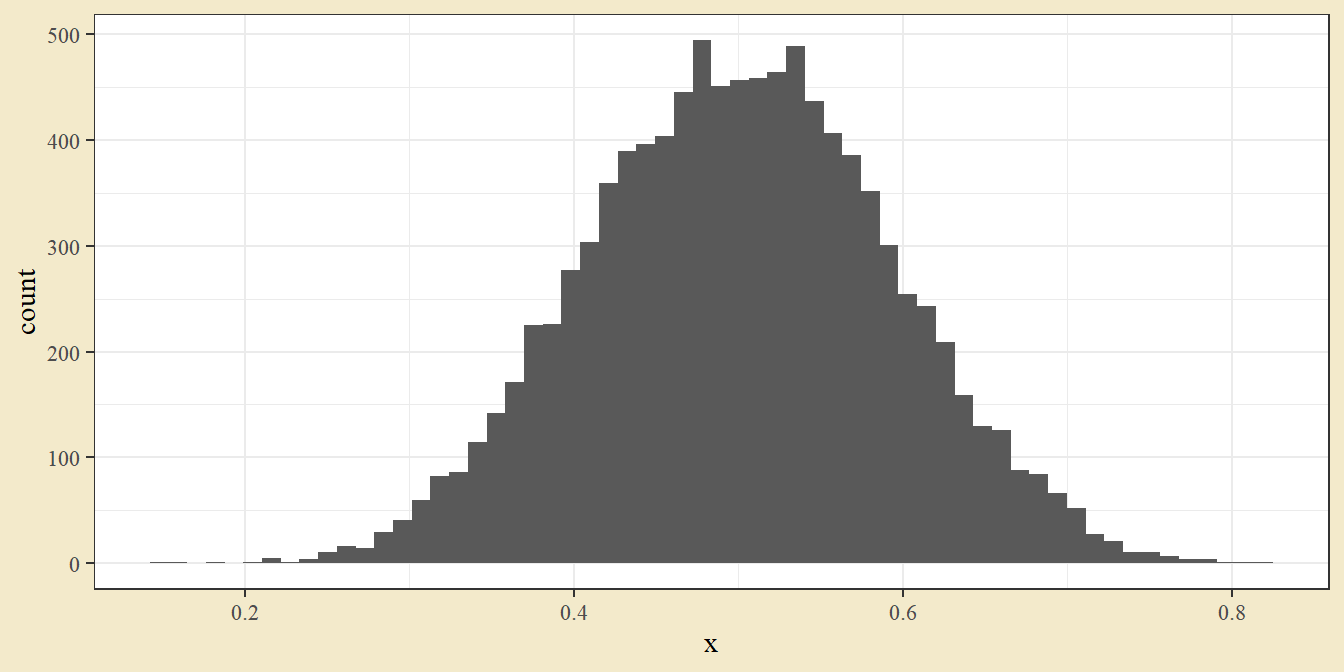
\includegraphics{R-anvisningar_files/figure-latex/unnamed-chunk-78-1} \end{center}

Medelvärdena följer en ungefärlig normalfördelning trots att den ursprungliga variabeln följer en likformig fördelning.

\hypertarget{uxf6vningar-1}{%
\section{Övningar}\label{uxf6vningar-1}}

\begin{exercise}[Binomial grobarhet]
I ett försöks sätts 10 frön med en grobarhetssannolikhet om 60 procent. Antal frön som gror följer då en binomialfördelning med \(N = 10\) och \(p = 0.6\), vilket kan skrivas \(X \sim Bin(10, 0.6)\).

a. Vad är sannolikheten att få exakt 6 groende frön, \(P(X = 6)\)?

b. Vad är sannolikheten att få högst 6 groende frön, \(P(X \leq 6)\)?

c. Beräkna slumpvariabelns \emph{fördelningsfunktion}.

d. Illustrera sannolikheterna från (c).

Ledning: \texttt{dbinom} och \texttt{pbinom} kan beräkna sannolikheter från en binomialfördelning.
\end{exercise}

\begin{hypothesis}[Binomial grobarhet]
Uppgiften kan lösas genom att ta fram sannolikheter med \texttt{dbinom} och \texttt{pbinom} med argumenten \texttt{size\ =\ 10} för tio frön och \texttt{prob\ =\ 0.6} för en grobarhet på 0.6

a.

\begin{Shaded}
\begin{Highlighting}[]
\FunctionTok{dbinom}\NormalTok{(}\AttributeTok{x =} \DecValTok{6}\NormalTok{, }\AttributeTok{size =} \DecValTok{10}\NormalTok{, }\AttributeTok{prob =} \FloatTok{0.6}\NormalTok{)}
\end{Highlighting}
\end{Shaded}

\begin{verbatim}
## [1] 0.2508227
\end{verbatim}

b.

\begin{Shaded}
\begin{Highlighting}[]
\FunctionTok{pbinom}\NormalTok{(}\DecValTok{6}\NormalTok{, }\AttributeTok{size =} \DecValTok{10}\NormalTok{, }\AttributeTok{prob =} \FloatTok{0.6}\NormalTok{)}
\end{Highlighting}
\end{Shaded}

\begin{verbatim}
## [1] 0.6177194
\end{verbatim}

c.

\begin{Shaded}
\begin{Highlighting}[]
\FunctionTok{tibble}\NormalTok{(}\AttributeTok{x =} \DecValTok{0}\SpecialCharTok{:}\DecValTok{10}\NormalTok{,}
\NormalTok{       Fördelningsfunktion }\OtherTok{=} \FunctionTok{pbinom}\NormalTok{(x, }\AttributeTok{size =} \DecValTok{10}\NormalTok{, }\AttributeTok{prob =} \FloatTok{0.6}\NormalTok{))}
\end{Highlighting}
\end{Shaded}

\begin{verbatim}
## # A tibble: 11 x 2
##        x Fördelningsfunktion
##    <int>               <dbl>
##  1     0            0.000105
##  2     1            0.00168 
##  3     2            0.0123  
##  4     3            0.0548  
##  5     4            0.166   
##  6     5            0.367   
##  7     6            0.618   
##  8     7            0.833   
##  9     8            0.954   
## 10     9            0.994   
## 11    10            1
\end{verbatim}

d.

\begin{Shaded}
\begin{Highlighting}[]
\NormalTok{dat }\OtherTok{\textless{}{-}} \FunctionTok{tibble}\NormalTok{(}\AttributeTok{x =} \DecValTok{0}\SpecialCharTok{:}\DecValTok{10}\NormalTok{,}
\NormalTok{       Fördelningsfunktion }\OtherTok{=} \FunctionTok{pbinom}\NormalTok{(x, }\AttributeTok{size =} \DecValTok{10}\NormalTok{, }\AttributeTok{prob =} \FloatTok{0.6}\NormalTok{),}
       \AttributeTok{Sannolikhetsfunktion =} \FunctionTok{dbinom}\NormalTok{(x, }\AttributeTok{size =} \DecValTok{10}\NormalTok{, }\AttributeTok{prob =} \FloatTok{0.6}\NormalTok{))}

\FunctionTok{ggplot}\NormalTok{(dat, }\FunctionTok{aes}\NormalTok{(x)) }\SpecialCharTok{+}
  \FunctionTok{geom\_bar}\NormalTok{(}\FunctionTok{aes}\NormalTok{(}\AttributeTok{y =}\NormalTok{ Fördelningsfunktion), }\AttributeTok{stat =} \StringTok{"identity"}\NormalTok{, }
           \AttributeTok{fill =} \StringTok{"pink"}\NormalTok{, }\AttributeTok{col =} \StringTok{"hotpink"}\NormalTok{, }\AttributeTok{width =} \FloatTok{0.5}\NormalTok{) }\SpecialCharTok{+}
  \FunctionTok{geom\_segment}\NormalTok{(}\FunctionTok{aes}\NormalTok{(}\AttributeTok{x =}\NormalTok{ x, }\AttributeTok{xend =}\NormalTok{ x, }
                   \AttributeTok{y =}\NormalTok{ Sannolikhetsfunktion, }\AttributeTok{yend =} \DecValTok{0}\NormalTok{)) }\SpecialCharTok{+}
  \FunctionTok{scale\_x\_continuous}\NormalTok{(}\AttributeTok{breaks =} \DecValTok{0}\SpecialCharTok{:}\DecValTok{10}\NormalTok{) }\SpecialCharTok{+}
  \FunctionTok{theme}\NormalTok{(}\AttributeTok{panel.background =} \FunctionTok{element\_rect}\NormalTok{(}\AttributeTok{fill =} \StringTok{"purple"}\NormalTok{), }
        \AttributeTok{panel.grid =} \FunctionTok{element\_blank}\NormalTok{())}
\end{Highlighting}
\end{Shaded}

\begin{center}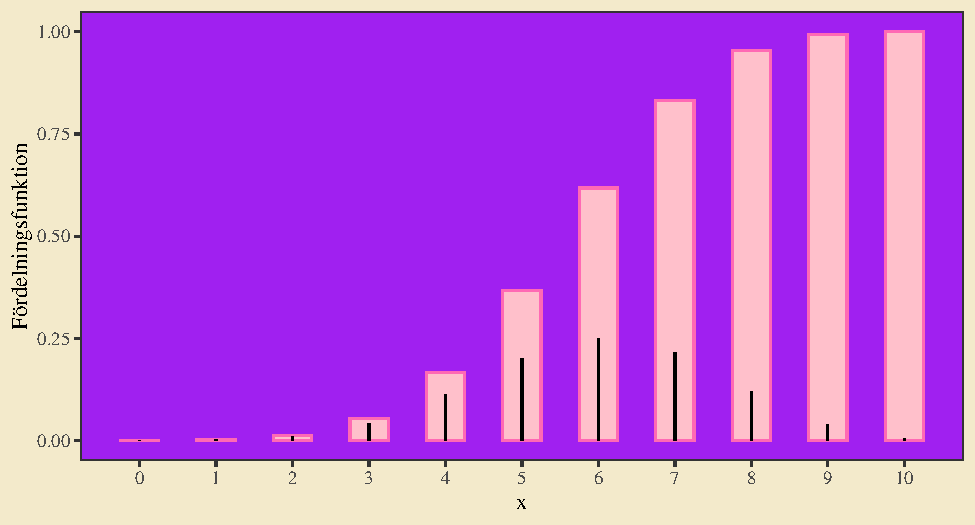
\includegraphics{R-anvisningar_files/figure-latex/unnamed-chunk-83-1} \end{center}

Illustration av fördelningsfunktionen (som breda staplar) med sannolikhetsfunktionen inritad som smala streck. Exempel på argument för val av färger för geom och tema. Sannolikheten i (a) (exakt 6 groende frön) ges av det svarta strecket vid 6 och sannolikheten i (b) (högst 6 groende frön) ges av den breda stapeln vid 6.
\end{hypothesis}

\begin{exercise}[Poissonfördelad klöver]
Antalet fyrklöver på en slumpmässigt vald kvadratmeter från en gräsmatta är poissonfördelad med väntevärde 1 per \(m^2\).

a. Hur stor är sannolikheten att en slumpmässigt vald \(m^2\) innehåller minst en fyrklöver, \(P(X \geq 1)\)? Exakt en fyrklöver, \(P(X = 1)\)?

b. Hur stor är sannolikheten att en slumpmässigt vald yta om 10 kvadratmeter innehåller exakt 10 fyrklöver?

Ledning: Summan av n stycken likadana poissonfördelade variabler är en poissonfördelad variabel med väntevärde givet av n gånger väntevärdet för den enskilda variabeln.

(Från Olsson, \emph{Biometri}.)
\end{exercise}

\begin{hypothesis}[Poissonfördelad klöver]
Sannolikheter för en poissonfördelning kan tas fram med \texttt{dpois} för sannolikhetsfunktionen eller \texttt{ppois} för fördelningsfunktionen.

a. Antal klöver på en kvadratmeter följer en poissonfördelning med \(\lambda = 1\). Sannolikheten för minst en fyrklöver kan beräknas genom ett minus sannolikheten för noll fyrklöver (utfallet noll fyrklöver är ett \emph{komplement} till utfallet en eller fler fyrklöver).

\begin{Shaded}
\begin{Highlighting}[]
\CommentTok{\# P(X \textgreater{}= 1) = 1 {-} P(X \textless{}= 0)}
\DecValTok{1} \SpecialCharTok{{-}} \FunctionTok{ppois}\NormalTok{(}\DecValTok{0}\NormalTok{, }\AttributeTok{lambda =} \DecValTok{1}\NormalTok{)}
\end{Highlighting}
\end{Shaded}

\begin{verbatim}
## [1] 0.6321206
\end{verbatim}

\begin{Shaded}
\begin{Highlighting}[]
\CommentTok{\# P(X = 1)}
\FunctionTok{dpois}\NormalTok{(}\DecValTok{1}\NormalTok{, }\AttributeTok{lambda =} \DecValTok{1}\NormalTok{)}
\end{Highlighting}
\end{Shaded}

\begin{verbatim}
## [1] 0.3678794
\end{verbatim}

b. Summan av poissonfördelade variabler är poissonfördelad med parametern \(\lambda\) given av summan av de ursprungliga variablernas parametervärden. Tio kvadratmeter kan ses som summan av tio stycken observationer av en kvadratmeter. Antal klöver på tio kvadratmeter bör därmed följa en poissonfördelning med \(\lambda = 10\).

\begin{Shaded}
\begin{Highlighting}[]
\CommentTok{\# Y \textasciitilde{} Po(lambda = 10)}
\FunctionTok{dpois}\NormalTok{(}\DecValTok{10}\NormalTok{, }\AttributeTok{lambda =} \DecValTok{10}\NormalTok{)}
\end{Highlighting}
\end{Shaded}

\begin{verbatim}
## [1] 0.12511
\end{verbatim}

Ungefär \(12.5\) procent.
\end{hypothesis}

\begin{exercise}[Sannolikheter från en normalfördelning]
Slumpvariabeln \(X\) är normalfördelad med medelvärde \(2\) och varians \(9\). Beräkna följande

a. \(P(X > 2.75)\)

b. \(P(X \leq 2.75)\)

c. \(P(X > 2.50)\)

d. \(P(2.30 < X < 2.45)\)

e. \(P(X > -0.02)\)

f. \(P(-0.02 < X < 1.80)\)

g. Bestäm värdet på x som uppfyller att \(P(X < x) = F(x) = 0.95\).

(Från Olsson, \emph{Biometri}. Samma som instuderingsuppgift 22.)
\end{exercise}

\begin{hypothesis}[Sannolikheter från en normalfördelning]
Sannolikheter från normalfördelningen kan tas fram med \texttt{pnorm}.

a. Notera att \emph{variansen} \(\sigma^2\) är \(9\) och att standardavvikelsen \(\sigma\) därmed är \(3\). Funktionen \texttt{pnorm} ger sannolikheten att ligga \emph{under} ett givet x-värde. För att beräkna \(P(X > 2.75)\) kan ta ett minus \(P(X < 2.75)\).

\begin{Shaded}
\begin{Highlighting}[]
\DecValTok{1} \SpecialCharTok{{-}} \FunctionTok{pnorm}\NormalTok{(}\FloatTok{2.75}\NormalTok{, }\AttributeTok{mean =} \DecValTok{2}\NormalTok{, }\AttributeTok{sd =} \DecValTok{3}\NormalTok{)}
\end{Highlighting}
\end{Shaded}

\begin{verbatim}
## [1] 0.4012937
\end{verbatim}

b. Direkt tillämpning av \texttt{pnorm}.

\begin{Shaded}
\begin{Highlighting}[]
\FunctionTok{pnorm}\NormalTok{(}\FloatTok{2.75}\NormalTok{, }\DecValTok{2}\NormalTok{, }\DecValTok{3}\NormalTok{)}
\end{Highlighting}
\end{Shaded}

\begin{verbatim}
## [1] 0.5987063
\end{verbatim}

c. Likt (a).

\begin{Shaded}
\begin{Highlighting}[]
\DecValTok{1} \SpecialCharTok{{-}} \FunctionTok{pnorm}\NormalTok{(}\FloatTok{2.5}\NormalTok{, }\DecValTok{2}\NormalTok{, }\DecValTok{3}\NormalTok{)}
\end{Highlighting}
\end{Shaded}

\begin{verbatim}
## [1] 0.4338162
\end{verbatim}

d. För att beräkna sannolikheten att ligga mellan två värden kan man ta skillnaden mellan två värden framräknade med \texttt{pnorm}.

\begin{Shaded}
\begin{Highlighting}[]
\FunctionTok{pnorm}\NormalTok{(}\FloatTok{2.45}\NormalTok{, }\DecValTok{2}\NormalTok{, }\DecValTok{3}\NormalTok{) }\SpecialCharTok{{-}} \FunctionTok{pnorm}\NormalTok{(}\FloatTok{2.30}\NormalTok{, }\DecValTok{2}\NormalTok{, }\DecValTok{3}\NormalTok{)}
\end{Highlighting}
\end{Shaded}

\begin{verbatim}
## [1] 0.01978986
\end{verbatim}

Om man vill illustrera en sannolikhet från en normalfördelning kan man beräkna normalfördelningskurvan med \texttt{dnorm} och sedan färglägga en sektion genom ett \texttt{geom\_ribbon} på filtrerad data. Exempel för (d).

\begin{Shaded}
\begin{Highlighting}[]
\NormalTok{dat }\OtherTok{\textless{}{-}} \FunctionTok{tibble}\NormalTok{(}\AttributeTok{x =} \FunctionTok{seq}\NormalTok{(}\SpecialCharTok{{-}}\DecValTok{7}\NormalTok{, }\DecValTok{11}\NormalTok{, }\FloatTok{0.01}\NormalTok{),}
\NormalTok{              Täthetsfunktion }\OtherTok{=} \FunctionTok{dnorm}\NormalTok{(x, }\DecValTok{2}\NormalTok{, }\DecValTok{3}\NormalTok{))}

\FunctionTok{ggplot}\NormalTok{(dat, }\FunctionTok{aes}\NormalTok{(x, Täthetsfunktion)) }\SpecialCharTok{+}
  \FunctionTok{geom\_line}\NormalTok{() }\SpecialCharTok{+}
  \FunctionTok{geom\_ribbon}\NormalTok{(}\FunctionTok{aes}\NormalTok{(}\AttributeTok{ymax =}\NormalTok{ Täthetsfunktion, }\AttributeTok{ymin =} \DecValTok{0}\NormalTok{), }
              \AttributeTok{data =}\NormalTok{ dat }\SpecialCharTok{\%\textgreater{}\%} \FunctionTok{filter}\NormalTok{(x }\SpecialCharTok{\textgreater{}} \FloatTok{2.30} \SpecialCharTok{\&}\NormalTok{ x }\SpecialCharTok{\textless{}} \FloatTok{2.45}\NormalTok{),}
              \AttributeTok{fill =} \StringTok{"turquoise"}\NormalTok{)}
\end{Highlighting}
\end{Shaded}

\begin{center}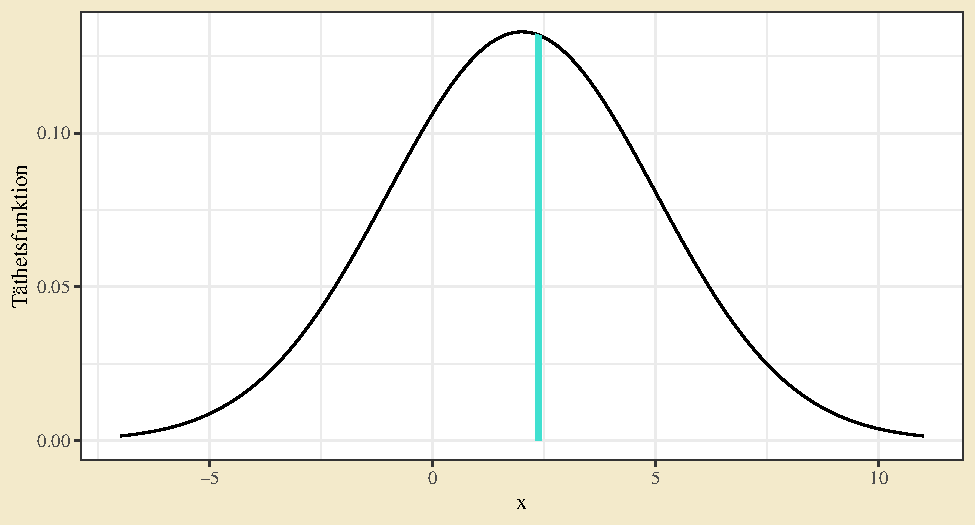
\includegraphics{R-anvisningar_files/figure-latex/unnamed-chunk-90-1} \end{center}

Den turkosa ytan motsvarar sannolikheten att \(X\) ger ett utfall mellan \(2.30\) och \(2.45\), sannolikheten uträknad i (d).

e.

\begin{Shaded}
\begin{Highlighting}[]
\DecValTok{1} \SpecialCharTok{{-}} \FunctionTok{pnorm}\NormalTok{(}\SpecialCharTok{{-}}\FloatTok{0.02}\NormalTok{, }\DecValTok{2}\NormalTok{, }\DecValTok{3}\NormalTok{)}
\end{Highlighting}
\end{Shaded}

\begin{verbatim}
## [1] 0.7496324
\end{verbatim}

f.

\begin{Shaded}
\begin{Highlighting}[]
\FunctionTok{pnorm}\NormalTok{(}\FloatTok{1.8}\NormalTok{, }\DecValTok{2}\NormalTok{, }\DecValTok{3}\NormalTok{) }\SpecialCharTok{{-}} \FunctionTok{pnorm}\NormalTok{(}\SpecialCharTok{{-}}\FloatTok{0.02}\NormalTok{, }\DecValTok{2}\NormalTok{, }\DecValTok{3}\NormalTok{)}
\end{Highlighting}
\end{Shaded}

\begin{verbatim}
## [1] 0.2230559
\end{verbatim}

g. Det sökta värdet är kvantil \(0.95\), ett värde sådant att 95 procent ligger under det värdet. Med en normalfördelning med medelvärde 2 och standardavvikelse 3 kan det tas fram med följande.

\begin{Shaded}
\begin{Highlighting}[]
\FunctionTok{qnorm}\NormalTok{(}\FloatTok{0.95}\NormalTok{, }\DecValTok{2}\NormalTok{, }\DecValTok{3}\NormalTok{) }\CommentTok{\# 2 och 3 anger medel 2 och standardavvikelse 3}
\end{Highlighting}
\end{Shaded}

\begin{verbatim}
## [1] 6.934561
\end{verbatim}

Tolkningen är att i en normal \(N(\mu = 2, \sigma^2 = 9)\) ligger 95 procent av ytan under \(6.9346\).

En illustration kan skapas med en datatabell med värden från fördelningens täthetsfunktion och \texttt{geom\_ribbon}.

\begin{Shaded}
\begin{Highlighting}[]
\NormalTok{dat }\OtherTok{\textless{}{-}} \FunctionTok{tibble}\NormalTok{(}\AttributeTok{x =} \FunctionTok{seq}\NormalTok{(}\SpecialCharTok{{-}}\DecValTok{7}\NormalTok{, }\DecValTok{11}\NormalTok{, }\FloatTok{0.01}\NormalTok{),}
\NormalTok{              Täthetsfunktion }\OtherTok{=} \FunctionTok{dnorm}\NormalTok{(x, }\DecValTok{2}\NormalTok{, }\DecValTok{3}\NormalTok{))}

\NormalTok{q\_95 }\OtherTok{\textless{}{-}} \FunctionTok{qnorm}\NormalTok{(}\FloatTok{0.95}\NormalTok{, }\DecValTok{2}\NormalTok{, }\DecValTok{3}\NormalTok{)}

\FunctionTok{ggplot}\NormalTok{(dat, }\FunctionTok{aes}\NormalTok{(x, Täthetsfunktion)) }\SpecialCharTok{+}
  \FunctionTok{geom\_line}\NormalTok{() }\SpecialCharTok{+}
  \FunctionTok{geom\_ribbon}\NormalTok{(}\FunctionTok{aes}\NormalTok{(}\AttributeTok{ymax =}\NormalTok{ Täthetsfunktion, }\AttributeTok{ymin =} \DecValTok{0}\NormalTok{), }
              \AttributeTok{data =}\NormalTok{ dat }\SpecialCharTok{\%\textgreater{}\%} \FunctionTok{filter}\NormalTok{(x }\SpecialCharTok{\textless{}}\NormalTok{ q\_95),}
              \AttributeTok{fill =} \StringTok{"turquoise"}\NormalTok{, }\AttributeTok{col =} \StringTok{"black"}\NormalTok{) }\SpecialCharTok{+}
  \FunctionTok{scale\_x\_continuous}\NormalTok{(}\AttributeTok{breaks =} \FunctionTok{c}\NormalTok{(}\SpecialCharTok{{-}}\DecValTok{5}\NormalTok{, }\DecValTok{0}\NormalTok{, }\DecValTok{5}\NormalTok{, }\FunctionTok{round}\NormalTok{(q\_95, }\DecValTok{3}\NormalTok{)))}
\end{Highlighting}
\end{Shaded}

\begin{center}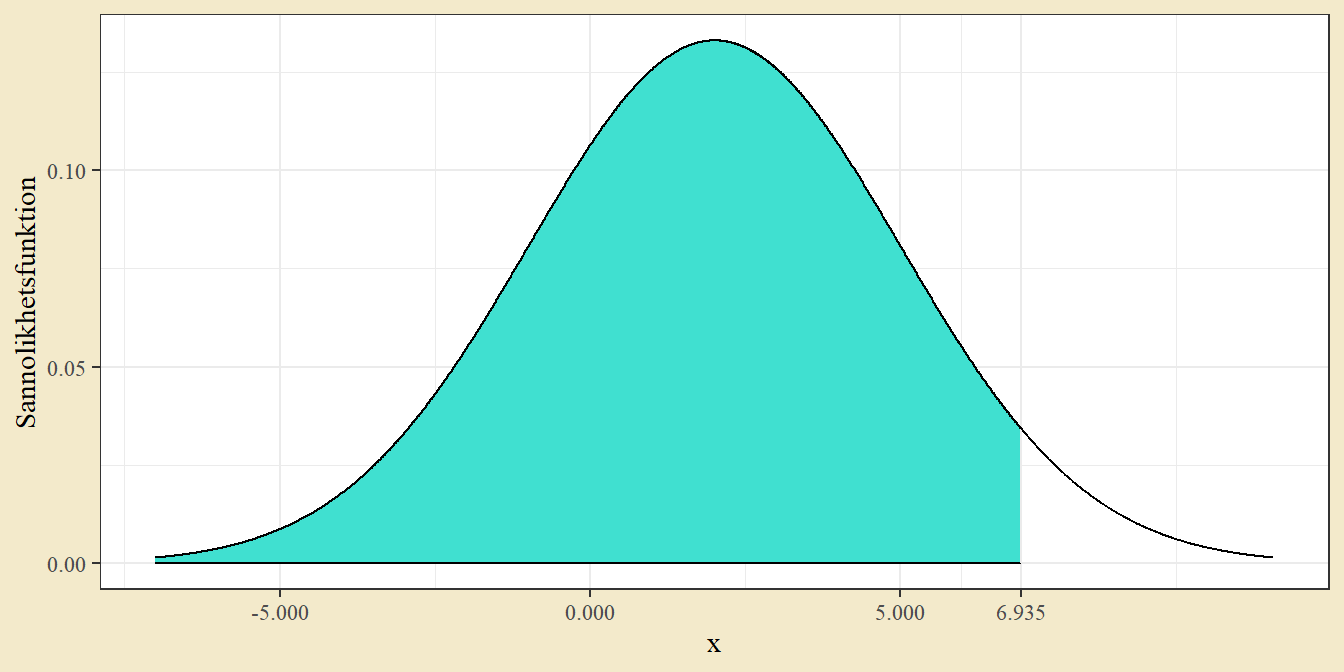
\includegraphics{R-anvisningar_files/figure-latex/unnamed-chunk-94-1} \end{center}

95 procent av ytan ligger under 6.935.
\end{hypothesis}

\begin{exercise}[Relativ frekvens]
Säg att man kastar ett häftstift och att sannolikheten att stiftet stannar med spetsen upp är 0.66. Simulera tusen häftstiftskast och beräkna den relativa frekvensen häftstiften hamnat med spetsen uppåt. Den relativa frekvensen för en serie värden ges av antalet positiva utfall delat på antalet kast för varje kast. Den relativa frekvensen efter 35 kast är till exempel antalet positiva utfall bland de 35, delat på 35.
Illustrera med ett linjediagram.

Ledning: tusen kast kan simuleras med \texttt{rbin(1000,\ 1,\ 0.66)}, vilket skapar tusen slumptal från en binomialfördelning där \(n = 1\) och \(p = 0.67\).
\end{exercise}

\begin{hypothesis}[Relativ frekvens]
För att beräkna och illustrera den relativa frekvensen skapas en \texttt{tibble} där den första kolumnen anger antalet kast vid varje steg, det vill säga en kolumn som anger ett till tusen. Därefter dras tusen slumptal enligt ledningen ovan. Därefter beräknas den \emph{kumulativa summan} - antalet positiva utfall upp till det kast som anges för raden. Och slutligen beräknas den relativa frekvensen genom att ta den kumulativa summan och dela med antalet kast.

\begin{Shaded}
\begin{Highlighting}[]
\NormalTok{dat }\OtherTok{\textless{}{-}} \FunctionTok{tibble}\NormalTok{(}\AttributeTok{Kast =} \DecValTok{1}\SpecialCharTok{:}\DecValTok{1000}\NormalTok{,}
              \AttributeTok{Utfall =} \FunctionTok{rbinom}\NormalTok{(}\DecValTok{1000}\NormalTok{, }\DecValTok{1}\NormalTok{, }\FloatTok{0.67}\NormalTok{),}
              \AttributeTok{Antal\_spets\_upp =} \FunctionTok{cumsum}\NormalTok{(Utfall),}
              \AttributeTok{Relativ\_frekvens =}\NormalTok{ Antal\_spets\_upp }\SpecialCharTok{/}\NormalTok{ Kast)}

\NormalTok{dat}
\end{Highlighting}
\end{Shaded}

\begin{verbatim}
## # A tibble: 1,000 x 4
##     Kast Utfall Antal_spets_upp Relativ_frekvens
##    <int>  <int>           <int>            <dbl>
##  1     1      1               1            1    
##  2     2      1               2            1    
##  3     3      1               3            1    
##  4     4      1               4            1    
##  5     5      1               5            1    
##  6     6      1               6            1    
##  7     7      1               7            1    
##  8     8      0               7            0.875
##  9     9      1               8            0.889
## 10    10      0               8            0.8  
## # ... with 990 more rows
\end{verbatim}

\begin{Shaded}
\begin{Highlighting}[]
\FunctionTok{ggplot}\NormalTok{(dat, }\FunctionTok{aes}\NormalTok{(Kast, Relativ\_frekvens)) }\SpecialCharTok{+}
  \FunctionTok{geom\_line}\NormalTok{() }\SpecialCharTok{+}
  \FunctionTok{geom\_hline}\NormalTok{(}\AttributeTok{yintercept =} \FloatTok{0.66}\NormalTok{, }\AttributeTok{col =} \StringTok{"red"}\NormalTok{, }\AttributeTok{alpha =} \FloatTok{0.7}\NormalTok{) }\SpecialCharTok{+}
  \FunctionTok{ylim}\NormalTok{(}\DecValTok{0}\NormalTok{,}\DecValTok{1}\NormalTok{)}
\end{Highlighting}
\end{Shaded}

\begin{center}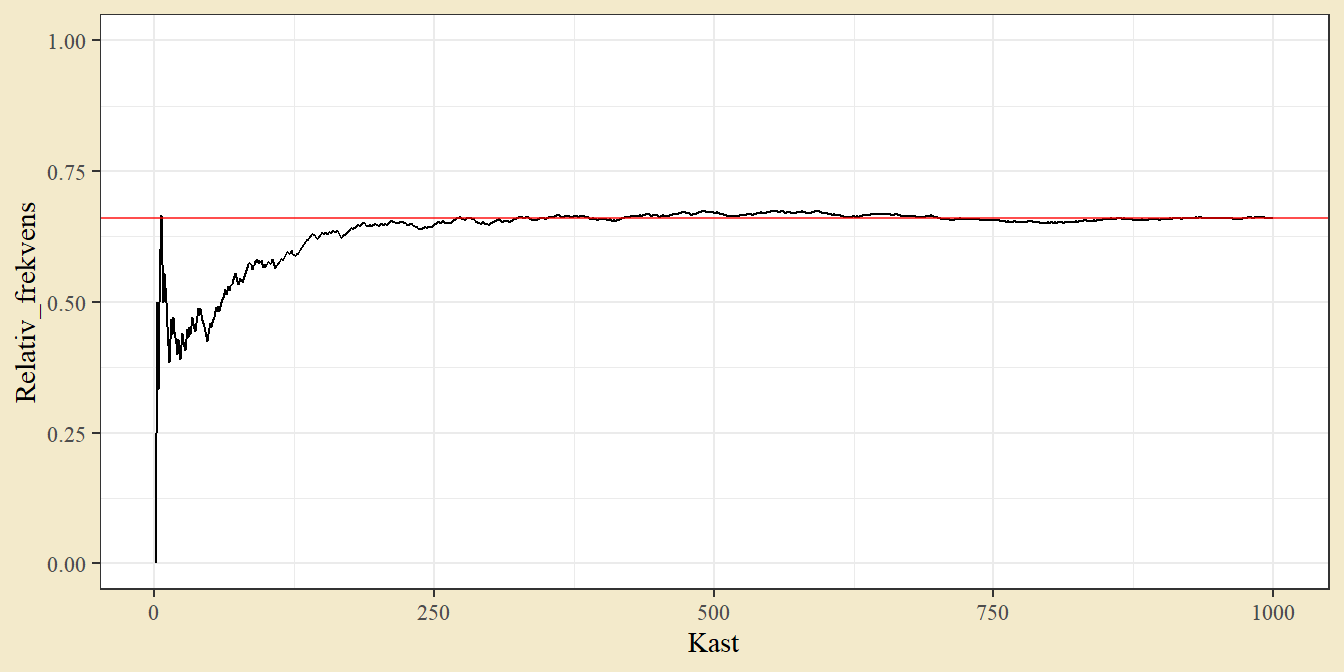
\includegraphics{R-anvisningar_files/figure-latex/unnamed-chunk-95-1} \end{center}

Den relativa frekvensen stabiliseras efter ett par hundra kast.
\end{hypothesis}

\begin{exercise}[Jämförelse mellan binomial och poisson]
Poissonfördelning kan ses som en approximation av en binomialfördelning när \(n\) är stort och \(p\) är litet. Poissonfördelningens parameter \(\lambda\) sätts vid approximation till binomialfördelningens populationsmedelvärde \(np\).

Ta som exempel en binomialfördelning men \(n = 10\) och \(p = 0.1\); dess väntevärde är \(10 \cdot 0.1 = 1\).
Beräkna sannolikheter från binomialfördelningen och motsvarande poissonfördelning. Jämför utfallen och illustrera med en passande graf.
\end{exercise}

\begin{hypothesis}[Jämförelse mellan binomial och poisson]
Fördelningen för binomial och poisson kan tas fram med \texttt{dbinom} respektive \texttt{dpois}.

\begin{Shaded}
\begin{Highlighting}[]
\NormalTok{dat }\OtherTok{\textless{}{-}} \FunctionTok{tibble}\NormalTok{(}\AttributeTok{x =} \DecValTok{0}\SpecialCharTok{:}\DecValTok{10}\NormalTok{,}
              \AttributeTok{Binomial =} \FunctionTok{dbinom}\NormalTok{(x, }\DecValTok{10}\NormalTok{, }\FloatTok{0.1}\NormalTok{),}
              \AttributeTok{Poisson =} \FunctionTok{dpois}\NormalTok{(x, }\DecValTok{1}\NormalTok{),}
              \AttributeTok{Differens =}\NormalTok{ Binomial }\SpecialCharTok{{-}}\NormalTok{ Poisson)}
\NormalTok{dat }\SpecialCharTok{\%\textgreater{}\%} \FunctionTok{round}\NormalTok{(}\DecValTok{3}\NormalTok{)}
\end{Highlighting}
\end{Shaded}

\begin{verbatim}
## # A tibble: 11 x 4
##        x Binomial Poisson Differens
##    <dbl>    <dbl>   <dbl>     <dbl>
##  1     0    0.349   0.368    -0.019
##  2     1    0.387   0.368     0.02 
##  3     2    0.194   0.184     0.01 
##  4     3    0.057   0.061    -0.004
##  5     4    0.011   0.015    -0.004
##  6     5    0.001   0.003    -0.002
##  7     6    0       0.001     0    
##  8     7    0       0         0    
##  9     8    0       0         0    
## 10     9    0       0         0    
## 11    10    0       0         0
\end{verbatim}

\begin{Shaded}
\begin{Highlighting}[]
\FunctionTok{ggplot}\NormalTok{(dat, }\FunctionTok{aes}\NormalTok{(x)) }\SpecialCharTok{+}
  \FunctionTok{geom\_point}\NormalTok{(}\FunctionTok{aes}\NormalTok{(}\AttributeTok{y =}\NormalTok{ Binomial), }\AttributeTok{col =} \StringTok{"red"}\NormalTok{) }\SpecialCharTok{+}
  \FunctionTok{geom\_point}\NormalTok{(}\FunctionTok{aes}\NormalTok{(}\AttributeTok{y =}\NormalTok{ Poisson), }\AttributeTok{col =} \StringTok{"green"}\NormalTok{)}
\end{Highlighting}
\end{Shaded}

\begin{center}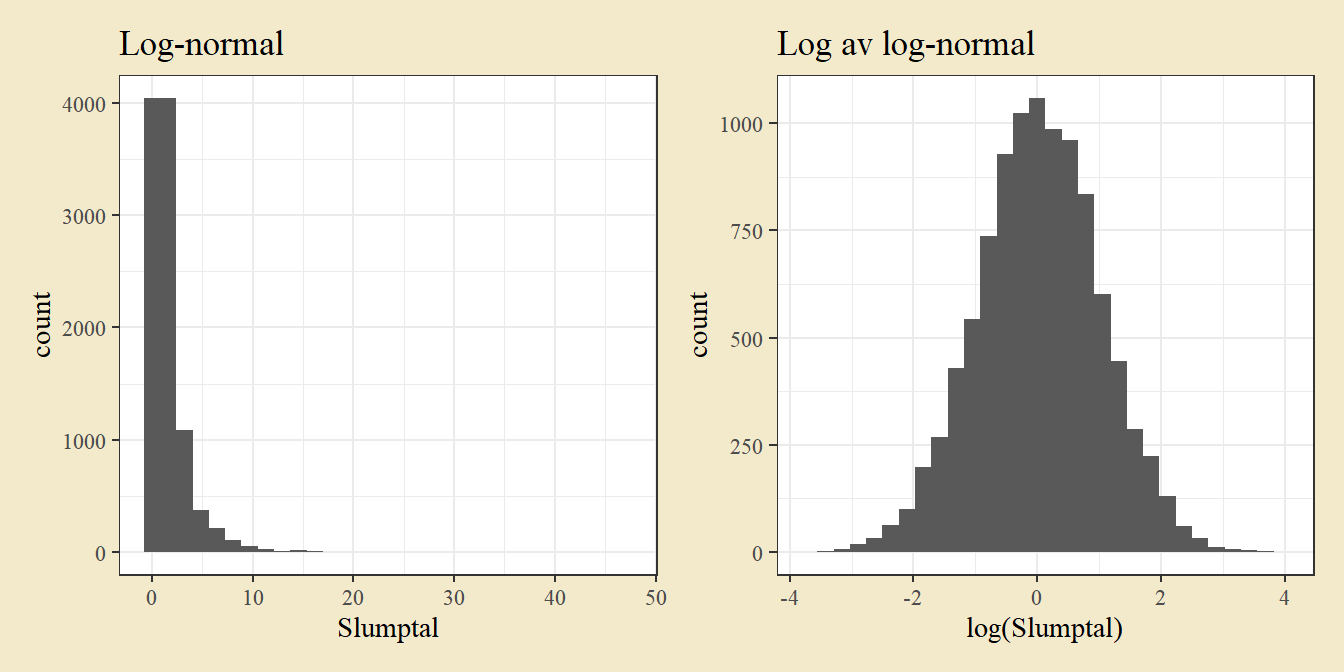
\includegraphics{R-anvisningar_files/figure-latex/unnamed-chunk-96-1} \end{center}

Fördelningarna är ganska lika. Relativt binomialen överskattar poissonfördelningen sannolikheten att få exakt 0 och överskattar sannolikheten att få exakt 1.
\end{hypothesis}

\begin{exercise}[Jämförelse mellan binomial och normal]
En av många orsaker till att normalfördelningen förekommer i tillämpningar är att både binomialfördelningen och poissonfördelningen kan approximeras med en normalfördelning om populationsmedelvärdet är stort. För att se exempel på detta kan man jämföra en binomialfördelning med en normalfördelning. Skapa en graf för en binomialfördelning med n = 100 och p = 0.4 med en överliggande normalfördelning med samma populationsmedelvärde och -varians, dvs. populationsmedelvärdet \(\mu = np = 100 \cdot 0.4 = 40\) och populationsvariansen \(\sigma^2 = n\cdot p \cdot (1-p) = 100 \cdot 0.4 \cdot 0.6 = 24\).
\end{exercise}

\begin{hypothesis}[Jämförelse mellan binomial och normal]
Funktionerna \texttt{dbinom} och \texttt{dnorm} kan användas för att ta fram funktionsvärden från binomial- och normalfördelning. Dessa kan sedan plottas i en ggplot genom \texttt{geom\_segment} för binomialen och \texttt{geom\_line} för den kontinuerliga normalfördelningen.

\begin{Shaded}
\begin{Highlighting}[]
\NormalTok{dat\_bin }\OtherTok{\textless{}{-}} \FunctionTok{tibble}\NormalTok{(}\AttributeTok{x =} \DecValTok{0}\SpecialCharTok{:}\DecValTok{100}\NormalTok{,}
                  \AttributeTok{Snlh =} \FunctionTok{dbinom}\NormalTok{(x, }\DecValTok{100}\NormalTok{, }\FloatTok{0.4}\NormalTok{))}
\NormalTok{dat\_norm }\OtherTok{\textless{}{-}} \FunctionTok{tibble}\NormalTok{(}\AttributeTok{x =} \FunctionTok{seq}\NormalTok{(}\DecValTok{0}\NormalTok{, }\DecValTok{100}\NormalTok{, }\AttributeTok{by =} \FloatTok{0.1}\NormalTok{),}
                   \AttributeTok{Snlh =} \FunctionTok{dnorm}\NormalTok{(x, }\AttributeTok{mean =} \DecValTok{40}\NormalTok{, }\AttributeTok{sd =} \FunctionTok{sqrt}\NormalTok{(}\DecValTok{24}\NormalTok{)))}

\FunctionTok{ggplot}\NormalTok{() }\SpecialCharTok{+}
  \FunctionTok{geom\_line}\NormalTok{(}\FunctionTok{aes}\NormalTok{(x, Snlh), }\AttributeTok{data =}\NormalTok{ dat\_norm, }\AttributeTok{col =} \StringTok{"blue"}\NormalTok{) }\SpecialCharTok{+}
  \FunctionTok{geom\_segment}\NormalTok{(}\FunctionTok{aes}\NormalTok{(}\AttributeTok{x =}\NormalTok{ x, }\AttributeTok{xend =}\NormalTok{ x, }\AttributeTok{y =} \DecValTok{0}\NormalTok{, }\AttributeTok{yend =}\NormalTok{Snlh), }
               \AttributeTok{data =}\NormalTok{ dat\_bin, }\AttributeTok{col =} \StringTok{"red"}\NormalTok{) }
\end{Highlighting}
\end{Shaded}

\begin{center}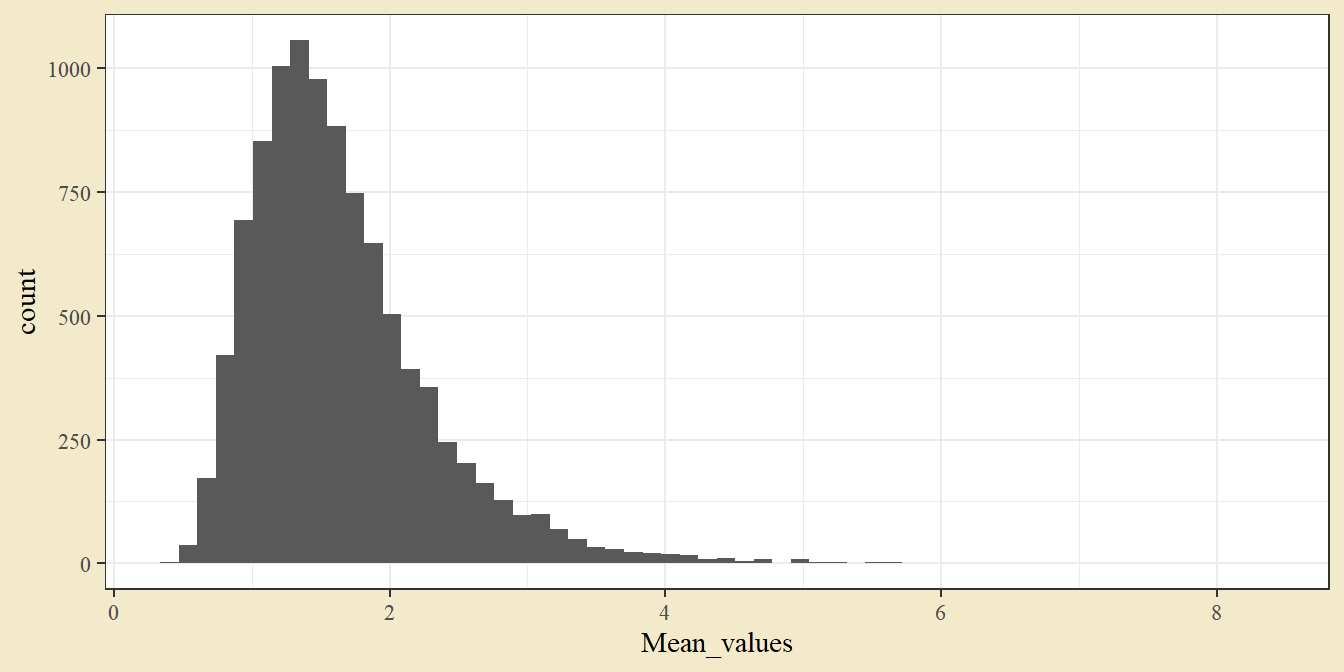
\includegraphics{R-anvisningar_files/figure-latex/unnamed-chunk-97-1} \end{center}

Normalkurvan (blå kontinuerlig linje) följer binomalfördelningen (röda staplar). Man kan också jämföra specifika sannolikheter, till exempel

\begin{Shaded}
\begin{Highlighting}[]
\CommentTok{\# Exakt 35 i binomialen}
\FunctionTok{dbinom}\NormalTok{(}\DecValTok{35}\NormalTok{, }\DecValTok{100}\NormalTok{, }\FloatTok{0.4}\NormalTok{) }\CommentTok{\# 0.0491}
\end{Highlighting}
\end{Shaded}

\begin{verbatim}
## [1] 0.04913282
\end{verbatim}

\begin{Shaded}
\begin{Highlighting}[]
\CommentTok{\# Mellan 34.5 och 35.5 i normalen}
\FunctionTok{pnorm}\NormalTok{(}\FloatTok{35.5}\NormalTok{, }\DecValTok{40}\NormalTok{, }\FunctionTok{sqrt}\NormalTok{(}\DecValTok{24}\NormalTok{)) }\SpecialCharTok{{-}} \FunctionTok{pnorm}\NormalTok{(}\FloatTok{34.5}\NormalTok{, }\DecValTok{40}\NormalTok{, }\FunctionTok{sqrt}\NormalTok{(}\DecValTok{24}\NormalTok{)) }\CommentTok{\# 0.0483}
\end{Highlighting}
\end{Shaded}

\begin{verbatim}
## [1] 0.04837712
\end{verbatim}

Sannolikheten för exakt 35 i binomialen ligger nära sannolikheten för utfall mellan 34.5 och 35.5 i normalfördelningen.
\end{hypothesis}

\begin{exercise}[Log-normal fördelning]
Ett exempel på en fördelning som är kontinuerlig, men inte normal, är en log-normal fördelning. En log-normal fördelning defineras av att den ger en normalfördelning efter att den logaritmeras - den är exponentialen av normalfördelningen. Dra 10000 slumptal från en log-normal fördelning (funktionen \texttt{rlnorm}) och illustrera med ett histogram. Ta logaritmen av datan och skapa histogrammet på nytt.
\end{exercise}

\begin{hypothesis}[Log-normal fördelning]

Funktionen \texttt{rlnorm} skapar slumptal från en log-normal fördelning. Två separata grafer plottar histogram över slumptalen och slumptalen efter log-transform.

\begin{Shaded}
\begin{Highlighting}[]
\NormalTok{dat }\OtherTok{\textless{}{-}} \FunctionTok{tibble}\NormalTok{(}\AttributeTok{Slumptal =} \FunctionTok{rlnorm}\NormalTok{(}\DecValTok{10000}\NormalTok{))}

\NormalTok{g1 }\OtherTok{\textless{}{-}} \FunctionTok{ggplot}\NormalTok{(dat, }\FunctionTok{aes}\NormalTok{(Slumptal)) }\SpecialCharTok{+} 
  \FunctionTok{geom\_histogram}\NormalTok{() }\SpecialCharTok{+}
  \FunctionTok{ggtitle}\NormalTok{(}\StringTok{"Log{-}normal"}\NormalTok{)}
  
\NormalTok{g2 }\OtherTok{\textless{}{-}} \FunctionTok{ggplot}\NormalTok{(dat, }\FunctionTok{aes}\NormalTok{(}\FunctionTok{log}\NormalTok{(Slumptal))) }\SpecialCharTok{+} 
  \FunctionTok{geom\_histogram}\NormalTok{() }\SpecialCharTok{+}
  \FunctionTok{ggtitle}\NormalTok{(}\StringTok{"Log av log{-}normal"}\NormalTok{)}

\FunctionTok{library}\NormalTok{(patchwork)}
\NormalTok{g1 }\SpecialCharTok{+}\NormalTok{ g2}
\end{Highlighting}
\end{Shaded}

\begin{center}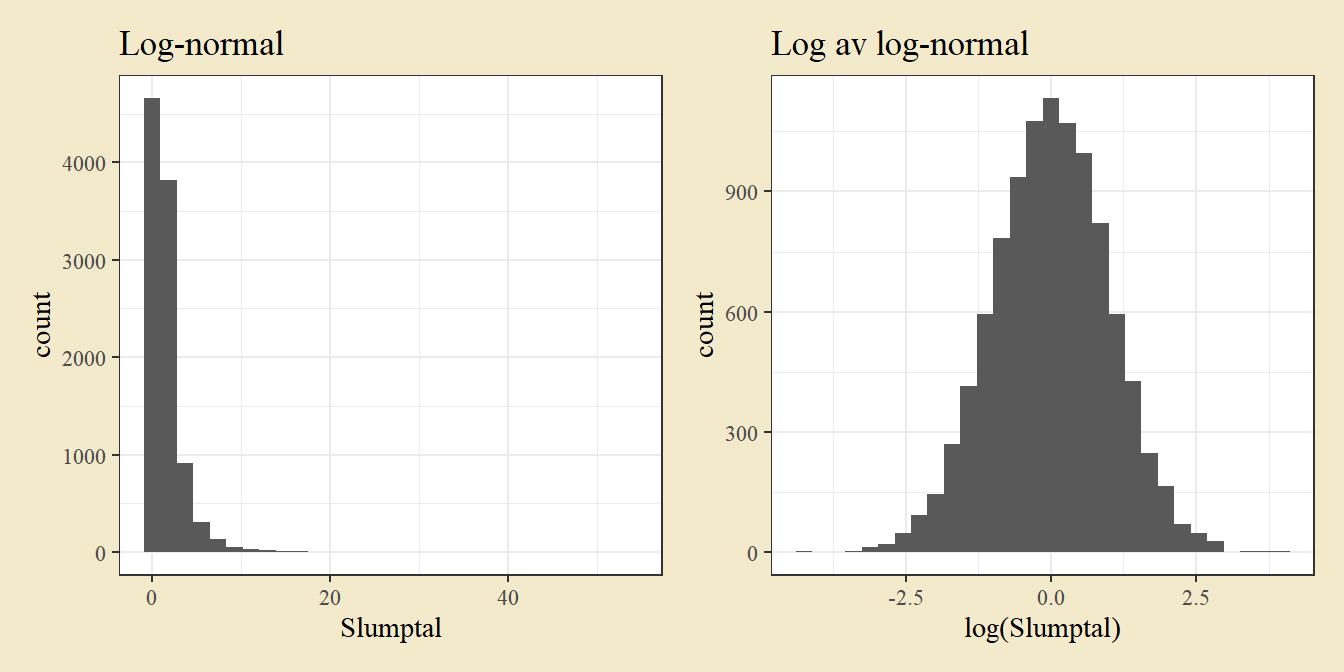
\includegraphics{R-anvisningar_files/figure-latex/unnamed-chunk-99-1} \end{center}

\end{hypothesis}

\begin{exercise}[Centrala gränsvärdesatsen]
Centrala gränsvärdesatsen ger att summor (och medelvärden) av flera likadana slumpvariabler följer en ungefärlig normalfördelning. Skriv en funktion som drar 10 observation från en log-normal fördelning och beräknar ett medelvärde. Dra 10000 upprepningar från den fördelningen och se om medelvärdena följer en normalfördelning. Gör samma sak men skriv funktionen så att den drar 1000 observationer och tar ett medelvärde.

Se anvisningarna för ett liknande exempel. Observera att detta är en svårare uppgift.
\end{exercise}

\begin{hypothesis}[Centrala gränsvärdesatsen]
En funktion som tar medelvärdet av tio observation skapas. Tiotusen sådana medelvärden beräknas och dessa illustreras med ett histogram.

\begin{Shaded}
\begin{Highlighting}[]
\NormalTok{mean\_of\_ten }\OtherTok{\textless{}{-}} \ControlFlowTok{function}\NormalTok{()\{}
\NormalTok{  x }\OtherTok{\textless{}{-}} \FunctionTok{rlnorm}\NormalTok{(}\DecValTok{10}\NormalTok{)}
  \FunctionTok{mean}\NormalTok{(x)}
\NormalTok{\}}

\NormalTok{means }\OtherTok{\textless{}{-}} \FunctionTok{replicate}\NormalTok{(}\DecValTok{10000}\NormalTok{, }\FunctionTok{mean\_of\_ten}\NormalTok{())}

\NormalTok{dat }\OtherTok{\textless{}{-}} \FunctionTok{tibble}\NormalTok{(}\AttributeTok{Mean\_values =}\NormalTok{ means)}

\FunctionTok{ggplot}\NormalTok{(dat, }\FunctionTok{aes}\NormalTok{(Mean\_values)) }\SpecialCharTok{+}
  \FunctionTok{geom\_histogram}\NormalTok{(}\AttributeTok{bins =} \DecValTok{60}\NormalTok{)}
\end{Highlighting}
\end{Shaded}

\begin{center}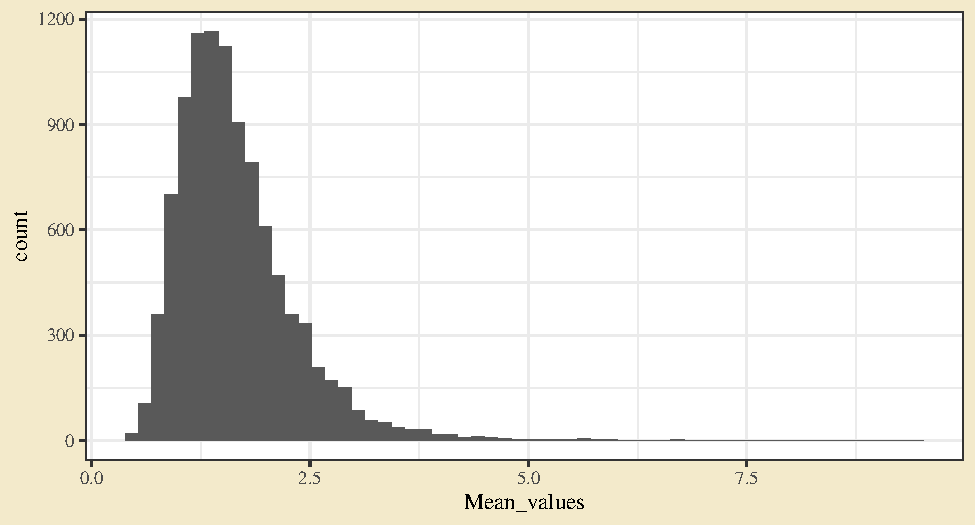
\includegraphics{R-anvisningar_files/figure-latex/unnamed-chunk-100-1} \end{center}

Histogrammet visar en klar skevhet.

\begin{Shaded}
\begin{Highlighting}[]
\NormalTok{mean\_of\_thousand }\OtherTok{\textless{}{-}} \ControlFlowTok{function}\NormalTok{()\{}
\NormalTok{  x }\OtherTok{\textless{}{-}} \FunctionTok{rlnorm}\NormalTok{(}\DecValTok{1000}\NormalTok{)}
  \FunctionTok{mean}\NormalTok{(x)}
\NormalTok{\}}

\NormalTok{means }\OtherTok{\textless{}{-}} \FunctionTok{replicate}\NormalTok{(}\DecValTok{10000}\NormalTok{, }\FunctionTok{mean\_of\_thousand}\NormalTok{())}

\NormalTok{dat }\OtherTok{\textless{}{-}} \FunctionTok{tibble}\NormalTok{(}\AttributeTok{Mean\_values =}\NormalTok{ means)}

\FunctionTok{ggplot}\NormalTok{(dat, }\FunctionTok{aes}\NormalTok{(Mean\_values)) }\SpecialCharTok{+}
  \FunctionTok{geom\_histogram}\NormalTok{(}\AttributeTok{bins =} \DecValTok{60}\NormalTok{)}
\end{Highlighting}
\end{Shaded}

\begin{center}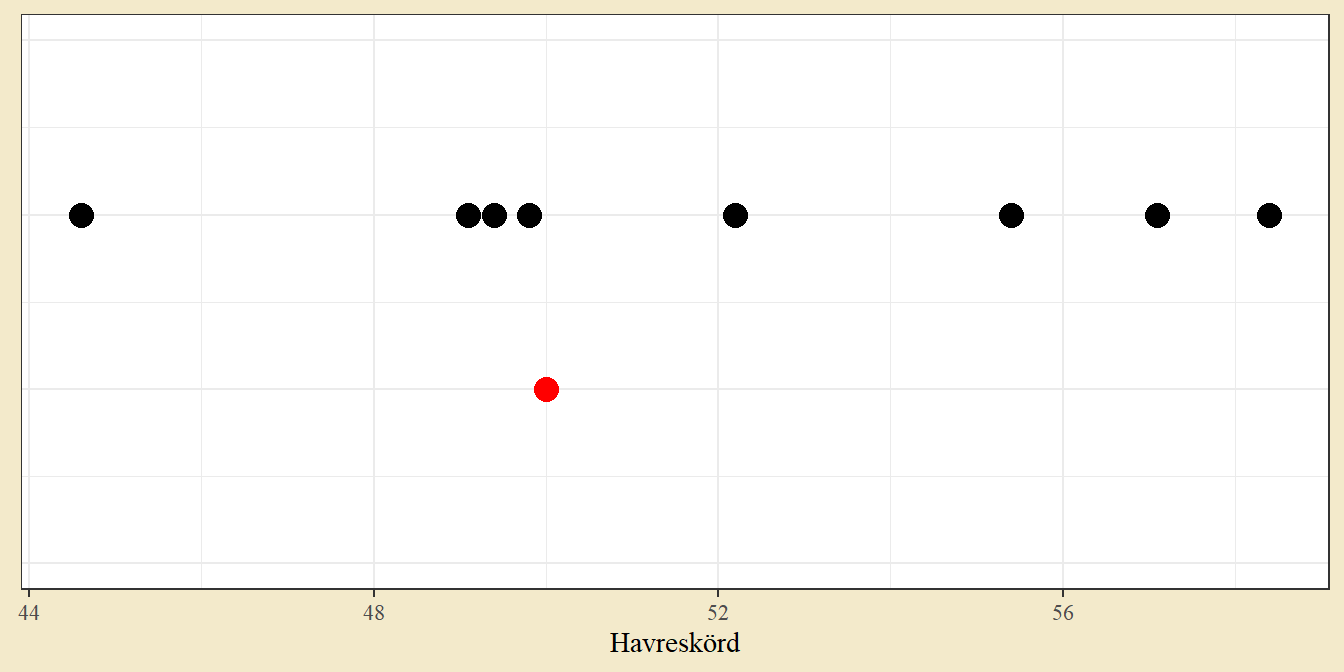
\includegraphics{R-anvisningar_files/figure-latex/unnamed-chunk-101-1} \end{center}

Histogrammet ligger närmare en typisk normalfördelning.
\end{hypothesis}

\begin{exercise}[Multiplicera med två eller addera två]
I en övningsuppsgift väcks frågan om det finns någon skillnad mellan att ta utfallet av en slumpvariabel och multiplicera med två, och att addera två slumpvariabler. Ta som exempel tre slumpvariabler \(X_1, X_2, X_3\) och låt dem alla följa en binomialfördelning med \(n = 100\) och \(p = 0.8\). Dra 10000 slumptal från respektive fördelning, beräkna \(2 \cdot X_1\) och \(X_2 + X_3\) och illustrera dessa beräknade variabler. Beräkna också väntevärde och standardavvikelse från de beräknade variablerna.
\end{exercise}

\begin{hypothesis}[Multiplicera med två eller addera två]
Tre variabler med slumptal konstrueras med \texttt{rbinom}. Därefter skapas två nya variabler, en genom summan av två av slumpvariablerna och en som den tredje slumpvariabeln multiplicerad med 2.

\begin{Shaded}
\begin{Highlighting}[]
\NormalTok{dat }\OtherTok{\textless{}{-}} \FunctionTok{tibble}\NormalTok{(}\AttributeTok{X1 =} \FunctionTok{rbinom}\NormalTok{(}\DecValTok{10000}\NormalTok{, }\AttributeTok{size =} \DecValTok{100}\NormalTok{, }\AttributeTok{prob =} \FloatTok{0.8}\NormalTok{),}
              \AttributeTok{X2 =} \FunctionTok{rbinom}\NormalTok{(}\DecValTok{10000}\NormalTok{, }\AttributeTok{size =} \DecValTok{100}\NormalTok{, }\AttributeTok{prob =} \FloatTok{0.8}\NormalTok{),}
              \AttributeTok{X3 =} \FunctionTok{rbinom}\NormalTok{(}\DecValTok{10000}\NormalTok{, }\AttributeTok{size =} \DecValTok{100}\NormalTok{, }\AttributeTok{prob =} \FloatTok{0.8}\NormalTok{)) }\SpecialCharTok{\%\textgreater{}\%} 
  \FunctionTok{mutate}\NormalTok{(}\AttributeTok{Mult\_by\_2 =} \DecValTok{2} \SpecialCharTok{*}\NormalTok{ X1,}
         \AttributeTok{Sum\_of\_two =}\NormalTok{ X2 }\SpecialCharTok{+}\NormalTok{ X3)}

\NormalTok{dat }\SpecialCharTok{\%\textgreater{}\%} 
  \FunctionTok{summarise\_all}\NormalTok{(mean)}
\end{Highlighting}
\end{Shaded}

\begin{verbatim}
## # A tibble: 1 x 5
##      X1    X2    X3 Mult_by_2 Sum_of_two
##   <dbl> <dbl> <dbl>     <dbl>      <dbl>
## 1  80.0  80.0  80.0      160.       160.
\end{verbatim}

\begin{Shaded}
\begin{Highlighting}[]
\NormalTok{dat }\SpecialCharTok{\%\textgreater{}\%} 
  \FunctionTok{summarise\_all}\NormalTok{(sd)}
\end{Highlighting}
\end{Shaded}

\begin{verbatim}
## # A tibble: 1 x 5
##      X1    X2    X3 Mult_by_2 Sum_of_two
##   <dbl> <dbl> <dbl>     <dbl>      <dbl>
## 1  4.03  4.00  4.02      8.06       5.67
\end{verbatim}

\begin{Shaded}
\begin{Highlighting}[]
\NormalTok{dat }\SpecialCharTok{\%\textgreater{}\%} 
  \FunctionTok{select}\NormalTok{(Mult\_by\_2, Sum\_of\_two) }\SpecialCharTok{\%\textgreater{}\%} 
  \FunctionTok{pivot\_longer}\NormalTok{(}\DecValTok{1}\SpecialCharTok{:}\DecValTok{2}\NormalTok{) }\SpecialCharTok{\%\textgreater{}\%} 
  \FunctionTok{ggplot}\NormalTok{(}\FunctionTok{aes}\NormalTok{(value, }\AttributeTok{fill =}\NormalTok{ name)) }\SpecialCharTok{+}
  \FunctionTok{geom\_bar}\NormalTok{() }\SpecialCharTok{+}
  \FunctionTok{facet\_wrap}\NormalTok{(}\SpecialCharTok{\textasciitilde{}}\NormalTok{ name)}
\end{Highlighting}
\end{Shaded}

\begin{center}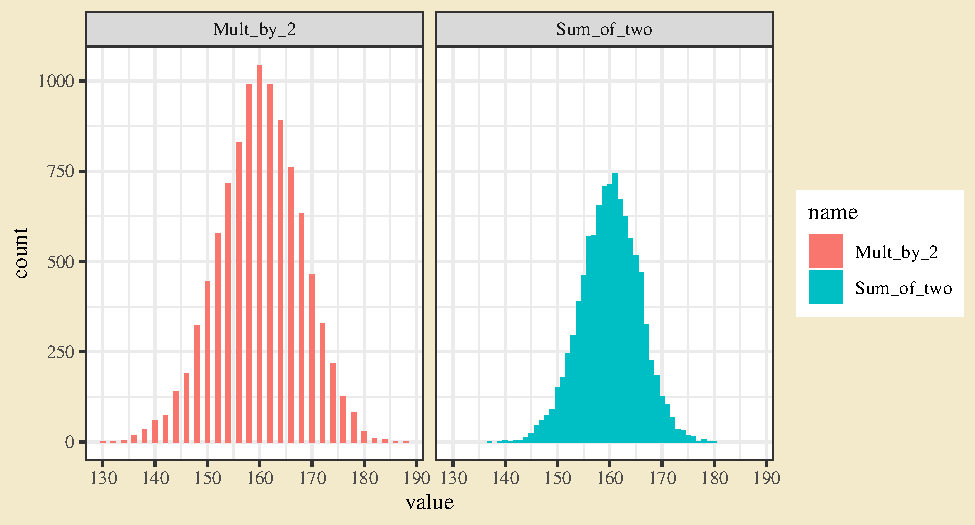
\includegraphics{R-anvisningar_files/figure-latex/unnamed-chunk-102-1} \end{center}

Stapeldiagrammet för fallet med en variabel multiplicerad med två ger högre staplar och större spridning än stapeldiagrammet med två summerade variabler. Diagrammet visar också hur vissa utfall inte kan inträffa i fallet med multiplikation, eftersom bara jämna utfall kan inträffa. Intuitivt kan man förstå den mindre spridningen för två summerade variabler med att ovanligt låga eller höga värden ofta kommer kvittas ut mot ett \emph{vanligt} värde.

Skillnaden märks också i beräkning av standardavvikelse. Den ursprungliga variabeln har en varians på \(np(1-p) = 100 \cdot 0.8 \cdot 0.2 = 16\) och därmed en standardavvikelse på\(\sqrt{16} = 4\). Multiplikation med två ger en slumpvariabel med den dubbla standardavvikelsen, alltså 8, medan addition av två likadana slumpvariabler ger en lägre standardavvikelse. För summor gäller att \emph{variansen av summan är summan av varianserna} (detta antar dock oberoende slumpvariabler) - här fås alltså att variansen av summan är \(16+16=32\) och att standardavvikelsen är \(\sqrt{32} = 5.6569\). Värdet i datan kommer förstås avvika något från den teoretiska beräkningen, eftersom det är slumptal.
\end{hypothesis}

\hypertarget{ett-stickprov}{%
\chapter{Ett stickprov}\label{ett-stickprov}}

\hypertarget{normalfuxf6rdelad-data-eller-stora-stickprov}{%
\section{Normalfördelad data (eller stora stickprov)}\label{normalfuxf6rdelad-data-eller-stora-stickprov}}

Om man har normalfördelad data och vill testa om datans medelvärde är skilt från något hypotetiskt värde \(\mu_0\) kan man använda ett t-test för ett stickprov. Testets hypoteser ges i det tvåsidiga fallet av

\[H_0: \mu = \mu_0 \qquad H_1: \mu \neq \mu_0.\]

Testet kan beräknas genom att beräkna testvärdet

\[t = \frac{\bar x - \mu_0}{s / \sqrt n}\]

och beräkna ett p-värde som sannolikheten i svansarna bortom det t-värdet, i en t-fördelning med \(n-1\) frihetsgrader.

Som exempel ges följande data på 8 observationer av havreskörd.

\begin{table}
\centering
\begin{tabular}[t]{rrrr}
\toprule
49.8 & 58.4 & 49.4 & 57.1\\
52.2 & 49.1 & 44.6 & 55.4\\
\bottomrule
\end{tabular}
\end{table}

Man vill testa om skörden är skild från 50, så hypoteser ges av

\[H_0: \mu = 50 \qquad H_1: \mu \neq 50.\]

Innan man utför testet kan det vara bra att ta en titt på datan och bilda en första uppfattning om nollhypotesens rimlighet. Man kan rita varje observation som en punkt i ett punktdiagram. Om det kan finnas överlappande punkter kan \texttt{geom\_dotplot} eller \texttt{geom\_count} användas för att separera eller notera överlappningar.

\begin{Shaded}
\begin{Highlighting}[]
\NormalTok{dat }\OtherTok{\textless{}{-}} \FunctionTok{c}\NormalTok{(}\FloatTok{49.8}\NormalTok{, }\FloatTok{58.4}\NormalTok{, }\FloatTok{49.4}\NormalTok{, }\FloatTok{57.1}\NormalTok{, }\FloatTok{52.2}\NormalTok{, }\FloatTok{49.1}\NormalTok{, }\FloatTok{44.6}\NormalTok{, }\FloatTok{55.4}\NormalTok{)}
\NormalTok{dat\_t }\OtherTok{\textless{}{-}} \FunctionTok{tibble}\NormalTok{(}\AttributeTok{x =}\NormalTok{ dat)}

\FunctionTok{ggplot}\NormalTok{(dat\_t, }\FunctionTok{aes}\NormalTok{(x, }\AttributeTok{y =} \DecValTok{0}\NormalTok{)) }\SpecialCharTok{+}
  \FunctionTok{geom\_point}\NormalTok{(}\AttributeTok{size =} \DecValTok{4}\NormalTok{) }\SpecialCharTok{+}
  \FunctionTok{annotate}\NormalTok{(}\StringTok{"point"}\NormalTok{, }\AttributeTok{x =} \DecValTok{50}\NormalTok{, }\AttributeTok{y =} \SpecialCharTok{{-}}\DecValTok{1}\NormalTok{, }\AttributeTok{col =} \StringTok{"red"}\NormalTok{, }\AttributeTok{size =} \DecValTok{4}\NormalTok{) }\SpecialCharTok{+}
  \FunctionTok{ylim}\NormalTok{(}\SpecialCharTok{{-}}\DecValTok{2}\NormalTok{,}\DecValTok{1}\NormalTok{) }\SpecialCharTok{+} \FunctionTok{xlab}\NormalTok{(}\StringTok{"Havreskörd"}\NormalTok{) }\SpecialCharTok{+}
  \FunctionTok{theme}\NormalTok{(}\AttributeTok{axis.text.y =} \FunctionTok{element\_blank}\NormalTok{(),}
        \AttributeTok{axis.ticks.y =} \FunctionTok{element\_blank}\NormalTok{(),}
        \AttributeTok{axis.title.y =} \FunctionTok{element\_blank}\NormalTok{())}
\end{Highlighting}
\end{Shaded}

\begin{center}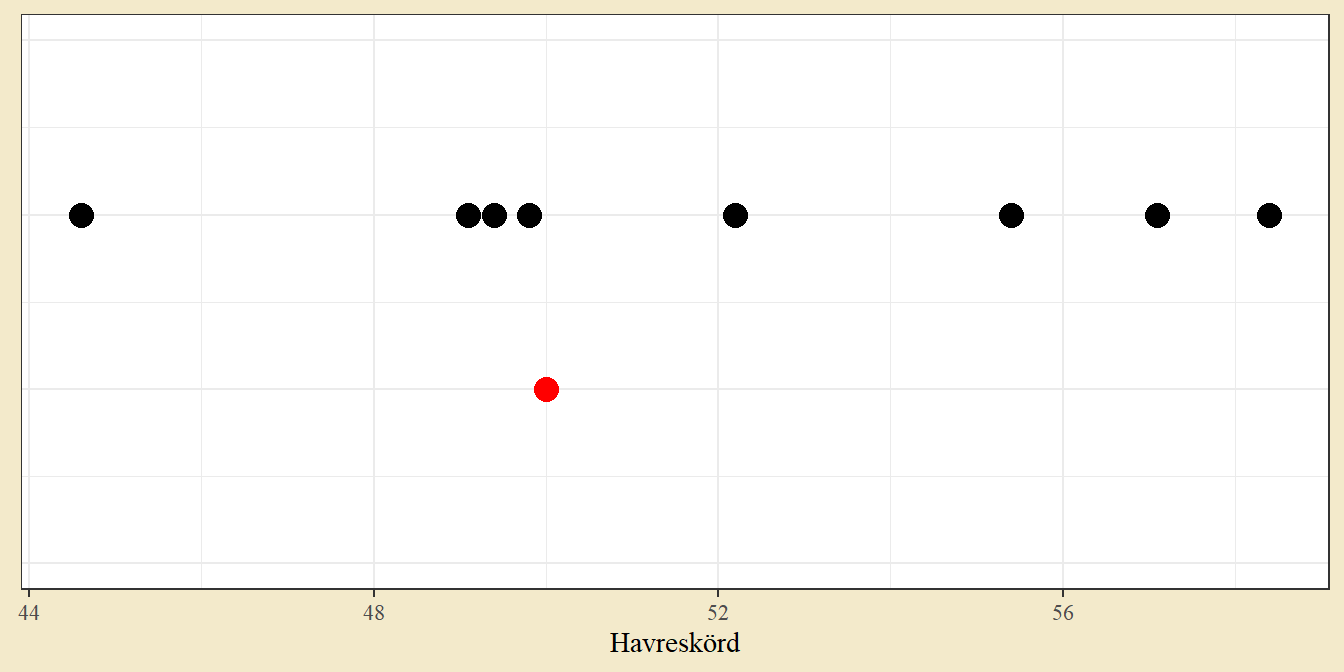
\includegraphics{R-anvisningar_files/figure-latex/unnamed-chunk-104-1} \end{center}

Det skattade medelvärdet är \(\bar x = 52.0\) och standardavvikelsen \(s = 4.68\). Teststorheten kan beräknas till

\[t = \frac{52 - 50}{4.68 / \sqrt 8} = 1.209\]

Testen kan genomföras i R med funktionen \texttt{t.test}.

\begin{Shaded}
\begin{Highlighting}[]
\NormalTok{dat }\OtherTok{\textless{}{-}} \FunctionTok{c}\NormalTok{(}\FloatTok{49.8}\NormalTok{, }\FloatTok{58.4}\NormalTok{, }\FloatTok{49.4}\NormalTok{, }\FloatTok{57.1}\NormalTok{, }\FloatTok{52.2}\NormalTok{, }\FloatTok{49.1}\NormalTok{, }\FloatTok{44.6}\NormalTok{, }\FloatTok{55.4}\NormalTok{)}
\FunctionTok{t.test}\NormalTok{(dat, }\AttributeTok{mu =} \DecValTok{50}\NormalTok{)}
\end{Highlighting}
\end{Shaded}

\begin{verbatim}
## 
##  One Sample t-test
## 
## data:  dat
## t = 1.2086, df = 7, p-value = 0.266
## alternative hypothesis: true mean is not equal to 50
## 95 percent confidence interval:
##  48.08713 55.91287
## sample estimates:
## mean of x 
##        52
\end{verbatim}

I funktionen anges datan \texttt{dat} och nollhypotesens värde \texttt{mu\ =\ 50}. Utskriften ger t-värdet till \(1.2086\) och p-värdet till \(0.266\). Det höga p-värdet ger att man inte förkastar nollhypotesen. Beräkningen av p-värdet kan illustreras med en t-fördelning.

\begin{Shaded}
\begin{Highlighting}[]
\NormalTok{test\_results }\OtherTok{\textless{}{-}} \FunctionTok{t.test}\NormalTok{(dat, }\AttributeTok{mu =} \DecValTok{50}\NormalTok{)}

\NormalTok{dat\_t }\OtherTok{\textless{}{-}} \FunctionTok{tibble}\NormalTok{(}\AttributeTok{x =} \FunctionTok{seq}\NormalTok{(}\SpecialCharTok{{-}}\DecValTok{4}\NormalTok{, }\DecValTok{4}\NormalTok{, }\FloatTok{0.01}\NormalTok{), }
                \AttributeTok{y =} \FunctionTok{dt}\NormalTok{(x, }\DecValTok{7}\NormalTok{))}

\FunctionTok{ggplot}\NormalTok{(dat\_t, }\FunctionTok{aes}\NormalTok{(x, y)) }\SpecialCharTok{+}
  \FunctionTok{geom\_line}\NormalTok{() }\SpecialCharTok{+}
  \FunctionTok{geom\_ribbon}\NormalTok{(}\FunctionTok{aes}\NormalTok{(}\AttributeTok{ymax =}\NormalTok{ y, }\AttributeTok{ymin =} \DecValTok{0}\NormalTok{), }\AttributeTok{fill =} \StringTok{"red3"}\NormalTok{, }
              \AttributeTok{data =}\NormalTok{ dat\_t }\SpecialCharTok{\%\textgreater{}\%} \FunctionTok{filter}\NormalTok{(x }\SpecialCharTok{\textless{}} \SpecialCharTok{{-}}\NormalTok{test\_results}\SpecialCharTok{$}\NormalTok{statistic)) }\SpecialCharTok{+}
  \FunctionTok{geom\_ribbon}\NormalTok{(}\FunctionTok{aes}\NormalTok{(}\AttributeTok{ymax =}\NormalTok{ y, }\AttributeTok{ymin =} \DecValTok{0}\NormalTok{), }\AttributeTok{fill =} \StringTok{"red3"}\NormalTok{, }
              \AttributeTok{data =}\NormalTok{ dat\_t }\SpecialCharTok{\%\textgreater{}\%} \FunctionTok{filter}\NormalTok{(x }\SpecialCharTok{\textgreater{}}\NormalTok{ test\_results}\SpecialCharTok{$}\NormalTok{statistic))}
\end{Highlighting}
\end{Shaded}

\begin{center}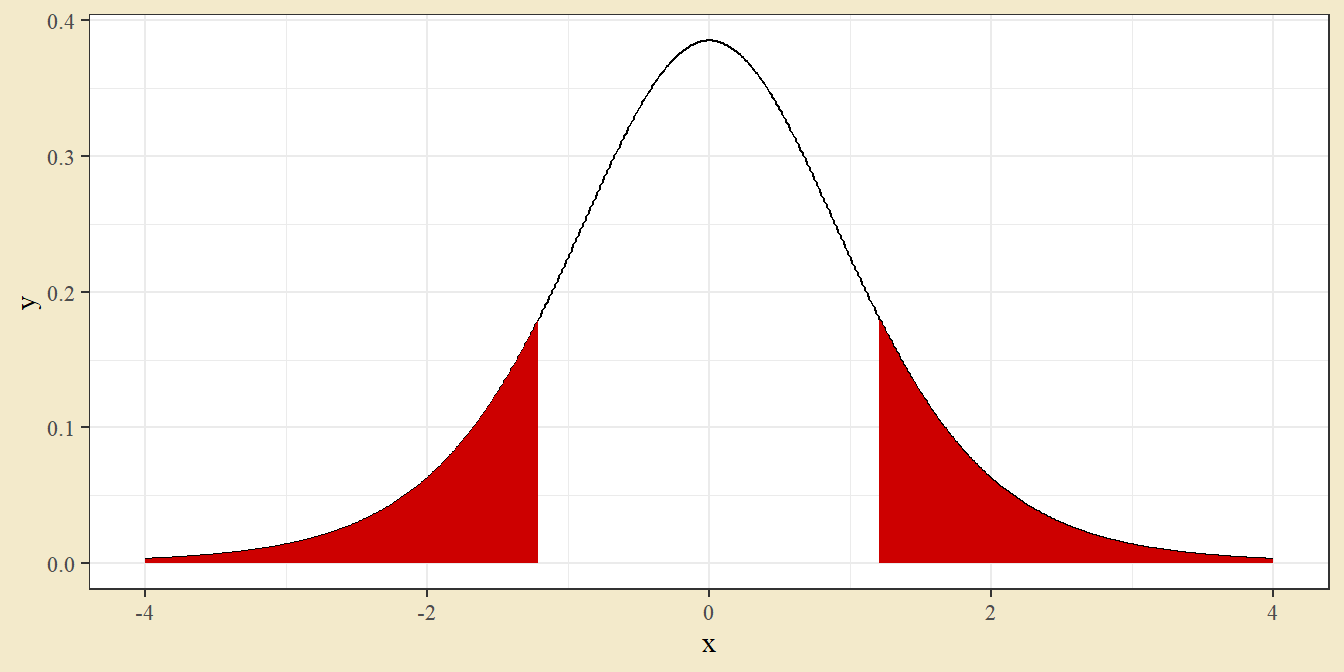
\includegraphics{R-anvisningar_files/figure-latex/unnamed-chunk-106-1} \end{center}

Notera hur man kan spara utfallet av \texttt{t.test} och sedan använda resultat direkt ur det objektet (här genom \texttt{test\_restults\$statistic} som ger teststorheten, men även \texttt{test\_results\$p.value} kan vara användbart). Testobjektets namn kan förstås vara något helt annat än \texttt{test\_results}.

Den röda arean i svansarna motsvarar p-värdet \(0.266\). Sannolikheten att få den observerade skillnaden mellan skattat medelvärde och nollhypotesens värde (52 respektive 50) även om det inte finns någon verklig skillnad är alltså ungefär en på fyra.

Utskriften från \texttt{t.test} ger också ett 95-procentigt konfidensintervall: \((48.09, 55.91)\). Tolkningen är att det sanna populationsmedelvärdet ligger i intervallet med 95 procents konfidens. Notera att nollhypotesens värde 50 ligger i intervallet.

\hypertarget{binuxe4r-data.-proportioner}{%
\section{Binär data. Proportioner}\label{binuxe4r-data.-proportioner}}

En skattad proportion kan ställas mot en nollhypotes genom ett \emph{binomialtest} eller \emph{z-test}. Ta som exempel att man samlar data om antal infekterade plantor i ett slumpmässigt urval av 50 och finner att 17 är infekterade. Man kan då testa nollhypotesen att den sanna populationsproportionen är 0.5,

\[H_0: p = 0.5 \qquad H_1: p \neq 0.5.\]

I R kan ett binomialtest utföras med \texttt{binom.test} och ett z-test (som bygger på en normalapproximation av binomialfördelningen) med \texttt{prop.test}. Det senare kan antingen utföras med eller utan en \emph{kontinuitetskorrektion}. Det test som beräknas för hand är oftast utan korrektionen.

\begin{Shaded}
\begin{Highlighting}[]
\FunctionTok{binom.test}\NormalTok{(}\DecValTok{17}\NormalTok{, }\DecValTok{50}\NormalTok{, }\AttributeTok{p =} \FloatTok{0.5}\NormalTok{)}
\end{Highlighting}
\end{Shaded}

\begin{verbatim}
## 
##  Exact binomial test
## 
## data:  17 and 50
## number of successes = 17, number of trials = 50, p-value = 0.03284
## alternative hypothesis: true probability of success is not equal to 0.5
## 95 percent confidence interval:
##  0.2120547 0.4876525
## sample estimates:
## probability of success 
##                   0.34
\end{verbatim}

\begin{Shaded}
\begin{Highlighting}[]
\FunctionTok{prop.test}\NormalTok{(}\DecValTok{17}\NormalTok{, }\DecValTok{50}\NormalTok{, }\AttributeTok{p =} \FloatTok{0.5}\NormalTok{, }\AttributeTok{correct =}\NormalTok{ F)}
\end{Highlighting}
\end{Shaded}

\begin{verbatim}
## 
##  1-sample proportions test without continuity correction
## 
## data:  17 out of 50, null probability 0.5
## X-squared = 5.12, df = 1, p-value = 0.02365
## alternative hypothesis: true p is not equal to 0.5
## 95 percent confidence interval:
##  0.2243695 0.4784617
## sample estimates:
##    p 
## 0.34
\end{verbatim}

\begin{Shaded}
\begin{Highlighting}[]
\FunctionTok{prop.test}\NormalTok{(}\DecValTok{17}\NormalTok{, }\DecValTok{50}\NormalTok{, }\AttributeTok{p =} \FloatTok{0.5}\NormalTok{, }\AttributeTok{correct =}\NormalTok{ T)}
\end{Highlighting}
\end{Shaded}

\begin{verbatim}
## 
##  1-sample proportions test with continuity correction
## 
## data:  17 out of 50, null probability 0.5
## X-squared = 4.5, df = 1, p-value = 0.03389
## alternative hypothesis: true p is not equal to 0.5
## 95 percent confidence interval:
##  0.2159464 0.4885541
## sample estimates:
##    p 
## 0.34
\end{verbatim}

Funktionernas argument är antal postiva utfall, det totala antalet utfall, och nollhypotesens värde. För \texttt{prop.test} anger argumentet \texttt{correct} om en korrektion ska utföras eller ej.
De tre testen ger liknande resultat, med p-värden kring 3 procent. Ett test på femprocentsnivån skulle alltså ge att nollhypotesen förkastas.

Utskrifterna ger också konfidensintervall, och precis som p-värden beror intervallet på fördelning och kontinuitetskorrektion. Tolkningen av intervallet är detsamma som i fallet med kontinuerlig data - den sanna populationsproportionen ligger i intervallet med 95 procents konfidens - men den exakta konstruktionen varierar beroende på detaljer i antaganden. För ett konfidensintervall som motsvarar det man vanligen beräknar för hand kan man använda \texttt{binomial}-paketet och funktionen \texttt{binom.confint}.

\begin{Shaded}
\begin{Highlighting}[]
\FunctionTok{library}\NormalTok{(binom)}
\FunctionTok{binom.confint}\NormalTok{(}\DecValTok{17}\NormalTok{, }\DecValTok{50}\NormalTok{, }\AttributeTok{methods =} \StringTok{"asymp"}\NormalTok{)}
\end{Highlighting}
\end{Shaded}

\begin{verbatim}
##       method  x  n mean    lower    upper
## 1 asymptotic 17 50 0.34 0.208697 0.471303
\end{verbatim}

Det interval som ges är kan beräknas genom att sätta \(\hat p = 17/50\) i uttrycket

\[\hat p \pm 1.96 \sqrt{\frac{\hat p (1 - \hat p)}{50}},\]

med ett litet avrundningsfel eftersom \(1.96\) är avrundat.

\hypertarget{nominal-eller-ordinal-data.-goodness-of-fit}{%
\section{Nominal eller ordinal data. Goodness-of-fit}\label{nominal-eller-ordinal-data.-goodness-of-fit}}

Goodness-of-fit-test testar fördelningen i insamlad data med en hypotetiskt fördelning. Teststorheten ges av

\[\chi^2 = \sum \frac{(O-E)^2}{E}\]

där summan går över alla utfall i fördelning, \(O\) är det observerade antalet i klassen och \(E\) är det förväntade antalet enligt den hypotetiska fördelningen. Under nollhypotesen följer teststorheten en \(\chi^2\)-fördelning.

Som exempel ges följande data på fågelobservationer.

\begin{table}
\centering
\begin{tabular}[t]{lr}
\toprule
Art & Antal\\
\midrule
Ladusvala & 237\\
Hussvala & 220\\
Backsvala & 143\\
\bottomrule
\end{tabular}
\end{table}

Totalt har man observerat 600 fåglar. Från tidigare års studier tror man att Ladusvalor och Hussvalor är lika vanliga, medan Backsvalar förekommer hälften så ofta - proportionerna skulle alltså vara 0.4, 0.4 respektive 0.2. Detta kan illustreras med ett stapeldiagram, med den hypotetiska fördelningen som punkter.

\begin{Shaded}
\begin{Highlighting}[]
\NormalTok{dat }\OtherTok{\textless{}{-}} \FunctionTok{tibble}\NormalTok{(}\AttributeTok{Art =} \FunctionTok{c}\NormalTok{(}\StringTok{"Ladusvala"}\NormalTok{, }\StringTok{"Hussvala"}\NormalTok{, }\StringTok{"Backsvala"}\NormalTok{),}
              \AttributeTok{Antal =} \FunctionTok{c}\NormalTok{(}\DecValTok{237}\NormalTok{, }\DecValTok{220}\NormalTok{, }\DecValTok{143}\NormalTok{))}

\FunctionTok{ggplot}\NormalTok{(dat, }\FunctionTok{aes}\NormalTok{(Art, Antal)) }\SpecialCharTok{+}
  \FunctionTok{geom\_bar}\NormalTok{(}\AttributeTok{stat =} \StringTok{"identity"}\NormalTok{) }\SpecialCharTok{+}
  \FunctionTok{geom\_point}\NormalTok{(}\FunctionTok{aes}\NormalTok{(}\AttributeTok{y =} \FunctionTok{c}\NormalTok{(}\FloatTok{0.4}\NormalTok{, }\FloatTok{0.4}\NormalTok{, }\FloatTok{0.2}\NormalTok{) }\SpecialCharTok{*} \DecValTok{600}\NormalTok{), }\AttributeTok{size =} \DecValTok{6}\NormalTok{)}
\end{Highlighting}
\end{Shaded}

\begin{center}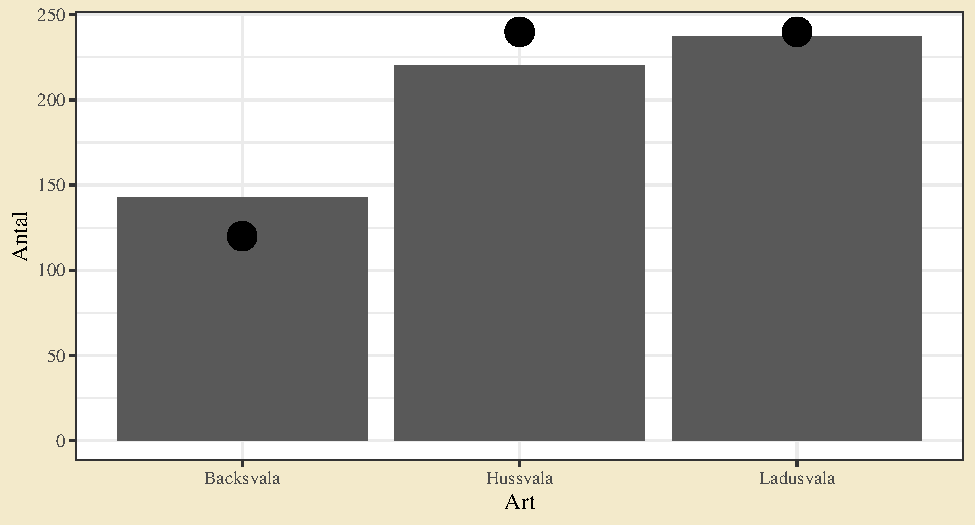
\includegraphics{R-anvisningar_files/figure-latex/unnamed-chunk-110-1} \end{center}

Grafen visar att hussvalor förekommer något mer sällan än väntat, medan backsvalor förekommer någon oftare.

För att genomföra testet i R används \texttt{chisq.test}. Funktionens ingångsvärden är den observerade datan och de teoretiska andelarna.

\begin{Shaded}
\begin{Highlighting}[]
\FunctionTok{chisq.test}\NormalTok{(dat}\SpecialCharTok{$}\NormalTok{Antal, }\AttributeTok{p =} \FunctionTok{c}\NormalTok{(}\FloatTok{0.4}\NormalTok{, }\FloatTok{0.4}\NormalTok{, }\FloatTok{0.2}\NormalTok{))}
\end{Highlighting}
\end{Shaded}

\begin{verbatim}
## 
##  Chi-squared test for given probabilities
## 
## data:  dat$Antal
## X-squared = 6.1125, df = 2, p-value = 0.04706
\end{verbatim}

Utskriften ger teststorheten \(\chi^2 = 6.1125\) och p-värdet \(0.04706\). I detta fall är p-värdet strax under fem procent - man skulle alltså förkasta nollhypotesen på signifikansnivån fem procent.

Utskriften ger också antalet frihetsgrader till två. I det här fallet ges den hypotetiska fördelningen av antagna sannolikheter, antalet frihetsgrader ges därför av antalet klasser minus ett. Men man kan också använda goodness-of-fit-test för att testa om data följer en viss typfördelning vars parameter beror på värden i data. Ett typiskt exempel på detta är test om data följer en poissonfördelning där man använder datan för att skatta \(\lambda\)-parametern i fördelningen. Antal frihetsgrader blir i sådana fall antalet klasser, minus antalet skattade parametrar, minus ett. Funktionen \texttt{chisq.test} kommer då ge fel antal frihetsgrader - p-värdet kan istället beräknas genom \texttt{pchisq}.

Ta som exempel följande frekvenstabell, beräknad från 500 observationer av en diskret variabel.

\begin{Shaded}
\begin{Highlighting}[]
\NormalTok{dat }\OtherTok{\textless{}{-}} \FunctionTok{tibble}\NormalTok{(}\AttributeTok{Utfall =} \DecValTok{0}\SpecialCharTok{:}\DecValTok{7}\NormalTok{, }
              \AttributeTok{Frekvens =} \FunctionTok{c}\NormalTok{(}\DecValTok{21}\NormalTok{,}\DecValTok{76}\NormalTok{,}\DecValTok{125}\NormalTok{,}\DecValTok{107}\NormalTok{,}\DecValTok{79}\NormalTok{,}\DecValTok{54}\NormalTok{,}\DecValTok{23}\NormalTok{,}\DecValTok{15}\NormalTok{))}
\FunctionTok{kable}\NormalTok{(dat)}
\end{Highlighting}
\end{Shaded}

\begin{table}
\centering
\begin{tabular}[t]{rr}
\toprule
Utfall & Frekvens\\
\midrule
0 & 21\\
1 & 76\\
2 & 125\\
3 & 107\\
4 & 79\\
\addlinespace
5 & 54\\
6 & 23\\
7 & 15\\
\bottomrule
\end{tabular}
\end{table}

Målet är att testa om datan följer en poissonfördelning. För att beräkna sannolikheter från en poissonfördelning behövs en skattning av parametern \(\lambda\). Detta ges av medelvärdet av de 600 observationerna, vilket kan beräknas genom att multiplicera utfallet med frekvensen, summera, och dela på 600.

\begin{Shaded}
\begin{Highlighting}[]
\NormalTok{lambda }\OtherTok{\textless{}{-}} \FunctionTok{sum}\NormalTok{(dat}\SpecialCharTok{$}\NormalTok{Utfall }\SpecialCharTok{*}\NormalTok{ dat}\SpecialCharTok{$}\NormalTok{Frekvens) }\SpecialCharTok{/} \DecValTok{500}
\NormalTok{lambda}
\end{Highlighting}
\end{Shaded}

\begin{verbatim}
## [1] 2.952
\end{verbatim}

Skattningen på \(\lambda\) är \(2.952\). Nästa steg är att beräkna sannolikheter från en poissonfördelning med det parametervärdet. För att sannolikheterna ska summera till ett justeras sannolikheten för det avslutande utfallet 7.

\begin{Shaded}
\begin{Highlighting}[]
\NormalTok{dat}\SpecialCharTok{$}\NormalTok{Sannolikheter }\OtherTok{\textless{}{-}} \FunctionTok{dpois}\NormalTok{(}\DecValTok{0}\SpecialCharTok{:}\DecValTok{7}\NormalTok{, lambda)}
\NormalTok{dat}\SpecialCharTok{$}\NormalTok{Sannolikheter[}\DecValTok{8}\NormalTok{] }\OtherTok{\textless{}{-}} \DecValTok{1} \SpecialCharTok{{-}} \FunctionTok{ppois}\NormalTok{(}\DecValTok{6}\NormalTok{, lambda)}
\FunctionTok{sum}\NormalTok{(dat}\SpecialCharTok{$}\NormalTok{Sannolikheter)}
\end{Highlighting}
\end{Shaded}

\begin{verbatim}
## [1] 1
\end{verbatim}

Data och nollhypotes kan illustreras med ett stapeldiagram där punkter anger förväntade värden från nollhypotesen.

\begin{Shaded}
\begin{Highlighting}[]
\FunctionTok{ggplot}\NormalTok{(dat, }\FunctionTok{aes}\NormalTok{(Utfall, Frekvens)) }\SpecialCharTok{+}
  \FunctionTok{geom\_bar}\NormalTok{(}\AttributeTok{stat =} \StringTok{"identity"}\NormalTok{) }\SpecialCharTok{+}
  \FunctionTok{geom\_point}\NormalTok{(}\FunctionTok{aes}\NormalTok{(}\AttributeTok{y =}\NormalTok{ Sannolikheter }\SpecialCharTok{*} \DecValTok{500}\NormalTok{))}
\end{Highlighting}
\end{Shaded}

\begin{center}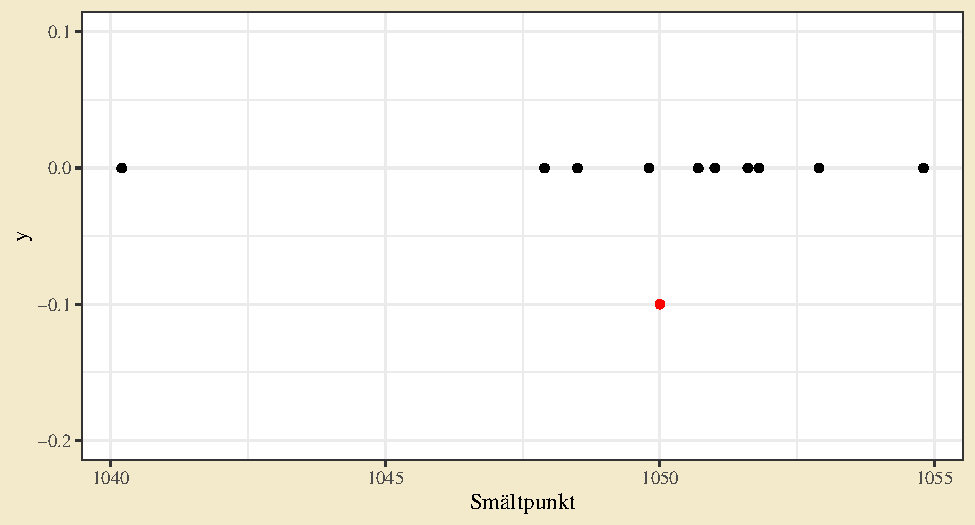
\includegraphics{R-anvisningar_files/figure-latex/unnamed-chunk-115-1} \end{center}

Data och nollhypotes verkar stämma ganska väl. Funktionen \texttt{chisq.test} kan användas för att beräkna teststorheten, men observera att antalet frihetsgrader nu blir fel - datan har åtta klasser, och då en parameter skattas i beräkningen av förväntade antal bör testet genomföras med \(8-1-1=6\) frihetsgrader. För att korrigera kan man ta fram teststorheten och beräkna p-värdet ur den korrekta fördelningen.

\begin{Shaded}
\begin{Highlighting}[]
\FunctionTok{chisq.test}\NormalTok{(dat}\SpecialCharTok{$}\NormalTok{Frekvens, }\AttributeTok{p =}\NormalTok{ dat}\SpecialCharTok{$}\NormalTok{Sannolikheter)}
\end{Highlighting}
\end{Shaded}

\begin{verbatim}
## 
##  Chi-squared test for given probabilities
## 
## data:  dat$Frekvens
## X-squared = 3.122, df = 7, p-value = 0.8735
\end{verbatim}

\begin{Shaded}
\begin{Highlighting}[]
\NormalTok{test\_result }\OtherTok{\textless{}{-}} \FunctionTok{chisq.test}\NormalTok{(dat}\SpecialCharTok{$}\NormalTok{Frekvens, }\AttributeTok{p =}\NormalTok{ dat}\SpecialCharTok{$}\NormalTok{Sannolikheter)}
\DecValTok{1} \SpecialCharTok{{-}} \FunctionTok{pchisq}\NormalTok{(test\_result}\SpecialCharTok{$}\NormalTok{statistic, }\AttributeTok{df =} \DecValTok{6}\NormalTok{)}
\end{Highlighting}
\end{Shaded}

\begin{verbatim}
## X-squared 
## 0.7933799
\end{verbatim}

I ett \(\chi^2\)-test är p-värdet sannolikheten i svansen till höger om teststorheten. Eftersom \texttt{pchisq}-funktionen beräknar sannolikheten till vänster, kan man ta komplementet genom att dra ifrån sannolikheten från ett.

\hypertarget{uxf6vningar-2}{%
\section{Övningar}\label{uxf6vningar-2}}

\begin{exercise}[Smältpunkt]
Någon mäter smältpunkter för legeringar av metall och får följande värden.

\begin{table}
\centering
\begin{tabular}[t]{rrrrr}
\toprule
1054.8 & 1052.9 & 1051.0 & 1049.8 & 1051.6\\
1047.9 & 1051.8 & 1048.5 & 1050.2 & 1050.7\\
\bottomrule
\end{tabular}
\end{table}

a. Beräkna ett 95-procentigt konfidensintervall för medelvärdet.

b. Genomför ett hypotestest för att testa om medelsmältpunkten är 1050 grader.
\end{exercise}

\begin{hypothesis}[Smältpunkt]
Datan kan importeras från excelfilen med uppgiftsdata.

\begin{Shaded}
\begin{Highlighting}[]
\NormalTok{dat }\OtherTok{\textless{}{-}}\NormalTok{ readxl}\SpecialCharTok{::}\FunctionTok{read\_excel}\NormalTok{(}\StringTok{"Data/Uppgiftsdata.xlsx"}\NormalTok{, }\AttributeTok{sheet =} \StringTok{"Smältpunkt"}\NormalTok{)}

\FunctionTok{ggplot}\NormalTok{(dat, }\FunctionTok{aes}\NormalTok{(Smältpunkt, }\DecValTok{0}\NormalTok{)) }\SpecialCharTok{+}
  \FunctionTok{geom\_point}\NormalTok{() }\SpecialCharTok{+}
  \FunctionTok{annotate}\NormalTok{(}\StringTok{"point"}\NormalTok{, }\AttributeTok{x =} \DecValTok{1050}\NormalTok{, }\AttributeTok{y =} \SpecialCharTok{{-}}\FloatTok{0.1}\NormalTok{, }\AttributeTok{col =} \StringTok{"red"}\NormalTok{) }\SpecialCharTok{+}
  \FunctionTok{ylim}\NormalTok{(}\SpecialCharTok{{-}}\FloatTok{0.2}\NormalTok{,}\FloatTok{0.1}\NormalTok{)}
\end{Highlighting}
\end{Shaded}

\begin{center}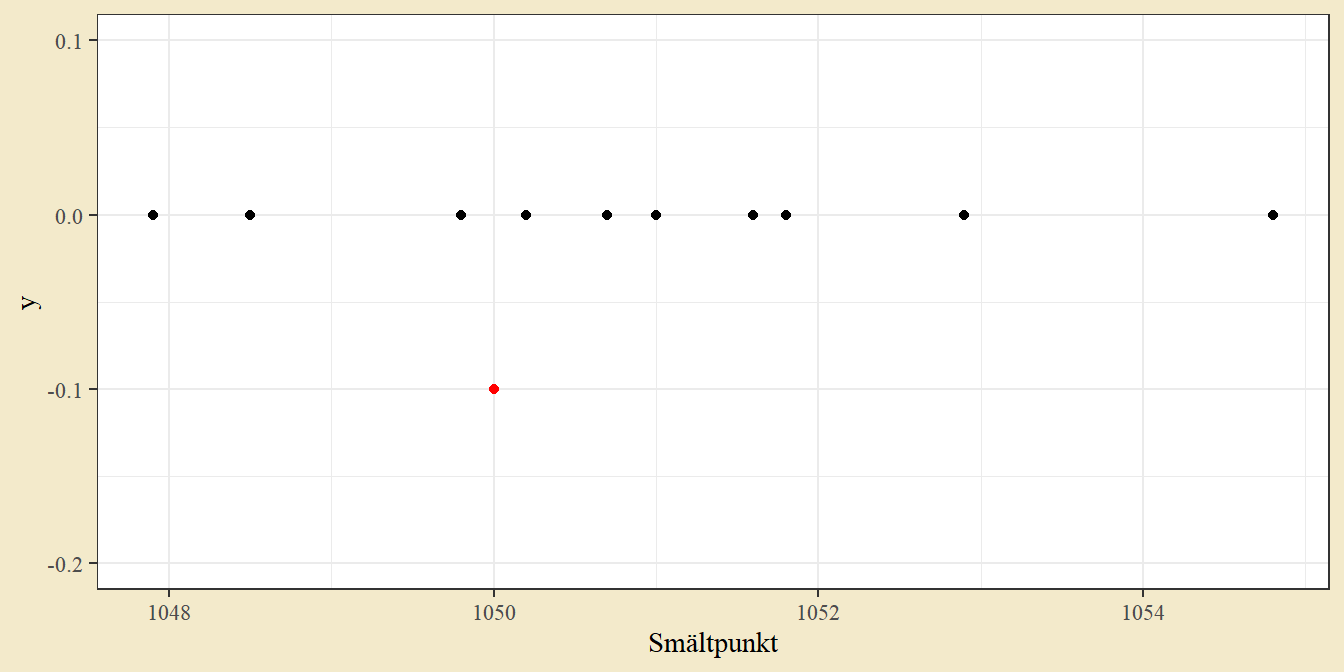
\includegraphics{R-anvisningar_files/figure-latex/unnamed-chunk-118-1} \end{center}

\begin{Shaded}
\begin{Highlighting}[]
\FunctionTok{t.test}\NormalTok{(dat}\SpecialCharTok{$}\NormalTok{Smältpunkt, }\AttributeTok{mu =} \DecValTok{1050}\NormalTok{)}
\end{Highlighting}
\end{Shaded}

\begin{verbatim}
## 
##  One Sample t-test
## 
## data:  dat$Smältpunkt
## t = 1.4345, df = 9, p-value = 0.1852
## alternative hypothesis: true mean is not equal to 1050
## 95 percent confidence interval:
##  1049.469 1052.371
## sample estimates:
## mean of x 
##   1050.92
\end{verbatim}

I bilden är varje svart punkt en observation och den röda punkten är nollhypotesens värde.

Testet ger ett högt p-värde, vilket tyder på att nollhypotesen inte bör förkastar. Ett 95-procentigt konfidensintervall ges av \((1047.08, 1052.76)\). Notera att det täcker nollhypotesens värde på 1050.
\end{hypothesis}

\begin{exercise}[Väderstation Falsterbo. Test och konfidensintervall]
Bland kursdatan finns en fil med temperaturmätningar från Falsterbo. Datan kan läsas in med följande kod.

\begin{Shaded}
\begin{Highlighting}[]
\NormalTok{dat }\OtherTok{\textless{}{-}} \FunctionTok{read\_csv2}\NormalTok{(}\StringTok{"Data/smhi{-}opendata\_1\_52230\_20210912\_114534.csv"}\NormalTok{, }\AttributeTok{skip =} \DecValTok{9}\NormalTok{) }\SpecialCharTok{\%\textgreater{}\%} 
  \FunctionTok{mutate}\NormalTok{(}\AttributeTok{Lufttemperatur =} \FunctionTok{as.numeric}\NormalTok{(Lufttemperatur))}
\end{Highlighting}
\end{Shaded}

Medeltemperatur 2000-2009 ges av följande tabell.

\begin{Shaded}
\begin{Highlighting}[]
\NormalTok{dat\_temp }\OtherTok{\textless{}{-}}\NormalTok{ dat }\SpecialCharTok{\%\textgreater{}\%} 
  \FunctionTok{mutate}\NormalTok{(Å}\AttributeTok{r =}\NormalTok{ lubridate}\SpecialCharTok{::}\FunctionTok{year}\NormalTok{(Datum)) }\SpecialCharTok{\%\textgreater{}\%} 
  \FunctionTok{filter}\NormalTok{(År }\SpecialCharTok{\%in\%} \DecValTok{2000}\SpecialCharTok{:}\DecValTok{2009}\NormalTok{) }\SpecialCharTok{\%\textgreater{}\%} 
  \FunctionTok{group\_by}\NormalTok{(År) }\SpecialCharTok{\%\textgreater{}\%} 
  \FunctionTok{summarise}\NormalTok{(}\AttributeTok{Medeltemperatur =} \FunctionTok{mean}\NormalTok{(Lufttemperatur)) }\SpecialCharTok{\%\textgreater{}\%} 
  \FunctionTok{mutate}\NormalTok{(}\AttributeTok{Medeltemperatur =} \FunctionTok{round}\NormalTok{(Medeltemperatur, }\DecValTok{2}\NormalTok{))}

\NormalTok{dat\_temp}
\end{Highlighting}
\end{Shaded}

\begin{Shaded}
\begin{Highlighting}[]
\FunctionTok{kable}\NormalTok{(dat\_temp)}
\end{Highlighting}
\end{Shaded}

\begin{table}
\centering
\begin{tabular}[t]{rr}
\toprule
År & Medeltemperatur\\
\midrule
2000 & 9.72\\
2001 & 8.98\\
2002 & 9.51\\
2003 & 8.89\\
2004 & 8.92\\
\addlinespace
2005 & 9.01\\
2006 & 9.63\\
2007 & 9.80\\
2008 & 9.81\\
2009 & 9.17\\
\bottomrule
\end{tabular}
\end{table}

Medelvärde och standardavvikelsen ges av följande.

\begin{Shaded}
\begin{Highlighting}[]
\FunctionTok{mean}\NormalTok{(dat\_temp}\SpecialCharTok{$}\NormalTok{Medeltemperatur)}
\end{Highlighting}
\end{Shaded}

\begin{verbatim}
## [1] 9.344
\end{verbatim}

\begin{Shaded}
\begin{Highlighting}[]
\FunctionTok{sd}\NormalTok{(dat\_temp}\SpecialCharTok{$}\NormalTok{Medeltemperatur)}
\end{Highlighting}
\end{Shaded}

\begin{verbatim}
## [1] 0.3852907
\end{verbatim}

a. Konstruera och tolka ett 95-procentigt konfidensintervall för medeltemperaturen under perioden.

b. Mätningarna från 1900-1949 ger en medeltemperatur på 8.42. Genomför ett passande t-test för att se om mätningarna från 2000-talet skiljer sig i medelvärde.

c. Titta på antalet mätningar per dag. Diskutera möjlig påverkan på testet i (b).
\end{exercise}

\begin{hypothesis}[Väderstation Falsterbo. Test och konfidensintervall]
a. Konfidensvallet kan tas fram med \texttt{t.test}. Den aggregerade datan med årsmedelvärden sparades tidigare som \texttt{dat\_temp}.

\begin{Shaded}
\begin{Highlighting}[]
\FunctionTok{t.test}\NormalTok{(dat\_temp}\SpecialCharTok{$}\NormalTok{Medeltemperatur)}
\end{Highlighting}
\end{Shaded}

\begin{verbatim}
## 
##  One Sample t-test
## 
## data:  dat_temp$Medeltemperatur
## t = 76.691, df = 9, p-value = 5.514e-14
## alternative hypothesis: true mean is not equal to 0
## 95 percent confidence interval:
##  9.06838 9.61962
## sample estimates:
## mean of x 
##     9.344
\end{verbatim}

Intervallet ges av \((9.06, 9.62)\). Populationsmedelvärdet för 2000-2009 ligger med 95-procents konfidens i det intervallet.

b. Funktionen \texttt{t.test} kan användas med nollhypotesens värde angivet med argumentet \texttt{mu}. Nollhypotesen är att populationsmedelvärdet \(\mu\) är 8.42.

\begin{Shaded}
\begin{Highlighting}[]
\FunctionTok{t.test}\NormalTok{(dat\_temp}\SpecialCharTok{$}\NormalTok{Medeltemperatur, }\AttributeTok{mu =} \FloatTok{8.42}\NormalTok{)}
\end{Highlighting}
\end{Shaded}

\begin{verbatim}
## 
##  One Sample t-test
## 
## data:  dat_temp$Medeltemperatur
## t = 7.5837, df = 9, p-value = 3.383e-05
## alternative hypothesis: true mean is not equal to 8.42
## 95 percent confidence interval:
##  9.06838 9.61962
## sample estimates:
## mean of x 
##     9.344
\end{verbatim}

Det låga p-värdet ger att nollhypotesen förkastas, vilket tyder på att medeltemperaturen 2000-2009 är skild från 8.42.

c. Man kan räkna antal observationer per dag med \texttt{count} och göra en linjegraf med \texttt{ggplot} och \texttt{geom\_line}.

\begin{Shaded}
\begin{Highlighting}[]
\NormalTok{dat }\SpecialCharTok{\%\textgreater{}\%} \FunctionTok{count}\NormalTok{(Datum) }\SpecialCharTok{\%\textgreater{}\%} \FunctionTok{ggplot}\NormalTok{(}\FunctionTok{aes}\NormalTok{(Datum, n)) }\SpecialCharTok{+} \FunctionTok{geom\_line}\NormalTok{()}
\end{Highlighting}
\end{Shaded}

\begin{center}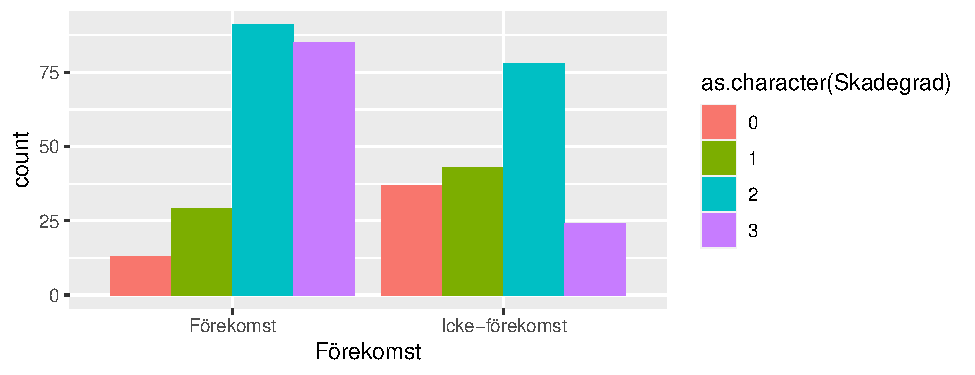
\includegraphics{R-anvisningar_files/figure-latex/unnamed-chunk-125-1} \end{center}

Antal observationer per dag är inte konstant. Om vissa dagar är uppmätta vid tider på dygnet då det är kallare eller varmare kan det ge en skevhet i mätningarna, vilket gör att jämförelsen mellan olika tider inte är rättvis. En lösning skulle kunna vara att ta värdet en viss tid på dygnet, en tid då det finns observationer för samtliga dagar. Det finns förstås också andra möjliga felkällor som påverkar en jämförelse över tid, t.ex. ändrade mätinstrument, små positionsförändringar, förändringar i kringliggande bebyggelse).
\end{hypothesis}

\begin{exercise}[Äppelträd]
I en undersökning av insektsskador på äppelträd har 6 plantor blivit vägda före och efter insektsdödande behandling. Syftet är att undersöka om behandlingen leder till förändrad vikt. Resultatet ges av följande tabell.

\begin{table}
\centering
\begin{tabular}[t]{lrrr}
\toprule
Träd & Före & Efter & Diff\\
\midrule
A & 271.1 & 311.2 & 40.1\\
B & 307.9 & 285.4 & -22.5\\
C & 305.9 & 320.9 & 15.0\\
D & 302.6 & 353.5 & 50.9\\
E & 263.4 & 358.0 & 94.6\\
\addlinespace
F & 277.7 & 286.1 & 8.4\\
\bottomrule
\end{tabular}
\end{table}

a. Gör ett test för att se om medelvärdet \emph{före} behandling är skilt från 310.

b. Beräkna ett konfidensintervall för skillnaden i populationsmedelvärden.
\end{exercise}

\begin{hypothesis}[Äppelträd]
Datan importeras från excelfilen med uppgiftsdata. Datan ändras till långform genom \texttt{pivot\_longer} och plottas med \texttt{ggplot}.

\begin{Shaded}
\begin{Highlighting}[]
\NormalTok{dat }\OtherTok{\textless{}{-}}\NormalTok{ readxl}\SpecialCharTok{::}\FunctionTok{read\_excel}\NormalTok{(}\StringTok{"Data/Uppgiftsdata.xlsx"}\NormalTok{, }\AttributeTok{sheet =} \StringTok{"Äppelträd"}\NormalTok{)}

\NormalTok{dat }\SpecialCharTok{\%\textgreater{}\%} 
  \FunctionTok{pivot\_longer}\NormalTok{(}\SpecialCharTok{{-}}\NormalTok{Träd) }\SpecialCharTok{\%\textgreater{}\%} 
  \FunctionTok{ggplot}\NormalTok{(}\FunctionTok{aes}\NormalTok{(name, value, }\AttributeTok{group =}\NormalTok{ Träd)) }\SpecialCharTok{+}
  \FunctionTok{geom\_point}\NormalTok{() }\SpecialCharTok{+}
  \FunctionTok{geom\_line}\NormalTok{()}
\end{Highlighting}
\end{Shaded}

\begin{center}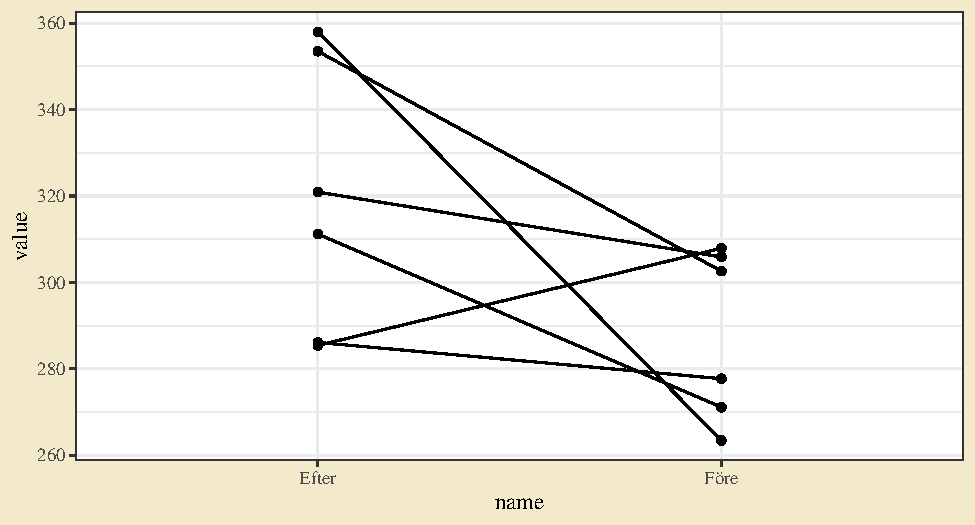
\includegraphics{R-anvisningar_files/figure-latex/unnamed-chunk-127-1} \end{center}

a.

\begin{Shaded}
\begin{Highlighting}[]
\FunctionTok{t.test}\NormalTok{(dat}\SpecialCharTok{$}\NormalTok{Före, }\AttributeTok{mu =} \DecValTok{310}\NormalTok{)}
\end{Highlighting}
\end{Shaded}

\begin{verbatim}
## 
##  One Sample t-test
## 
## data:  dat$Före
## t = -2.733, df = 5, p-value = 0.04113
## alternative hypothesis: true mean is not equal to 310
## 95 percent confidence interval:
##  267.5012 308.6988
## sample estimates:
## mean of x 
##     288.1
\end{verbatim}

Testet ger ett p-värde på \(0.041\). Nollhypotesen förkastas på femprocentsnivån men ej på enprocentsnivån.

b.

\begin{Shaded}
\begin{Highlighting}[]
\FunctionTok{t.test}\NormalTok{(dat}\SpecialCharTok{$}\NormalTok{Före, dat}\SpecialCharTok{$}\NormalTok{Efter, }\AttributeTok{paired =}\NormalTok{ T)}
\end{Highlighting}
\end{Shaded}

\begin{verbatim}
## 
##  Paired t-test
## 
## data:  dat$Före and dat$Efter
## t = -1.8855, df = 5, p-value = 0.118
## alternative hypothesis: true difference in means is not equal to 0
## 95 percent confidence interval:
##  -73.45961  11.29295
## sample estimates:
## mean of the differences 
##               -31.08333
\end{verbatim}

Konfidensintervallet ges av \((-73.46, 11.29)\). Den sanna behandlingsskillnaden ligger med 95 procents konfidens i det intervallet.
\end{hypothesis}

\begin{exercise}[Simulering, hypotestest]
Slumptal kan användas för att undersöka hypotestestens egenskaper. Skriv en funktion som genererar 100 slumptal från en normalfördelning med populationsmedelvärdet 0, testar mot nollhypotesen \(\mu_0 = 0\) i ett t-test, och ger ut p-värdet från det testet. Generera 10000 körningar av funktionen och illustrera p-värdena med ett histogram.

Upprepa samma procedur men dra denna gång slumptal från en normalfördelning med populationsmedelvärdet 0.1 (använs samma nollhypotes som tidigare \(\mu_0 = 0\)). Hur stor andel av de 10000 simuleringarna resulterar i ett p-värde under 0.05?
\end{exercise}

\begin{hypothesis}[Simulering hypotestest]
Här konstrueras en funktion som drar hundra slumpvärden, testar om medelvärdet är skilt från noll, och ger ut p-värdet från testet. Funktionen replikeras 10000 gånger och de resulterande p-värdena illustreras med ett histogram.

\begin{Shaded}
\begin{Highlighting}[]
\NormalTok{p\_values\_when\_mean\_0 }\OtherTok{\textless{}{-}} \ControlFlowTok{function}\NormalTok{()\{}
\NormalTok{  x }\OtherTok{\textless{}{-}} \FunctionTok{rnorm}\NormalTok{(}\DecValTok{100}\NormalTok{, }\AttributeTok{mean =} \DecValTok{0}\NormalTok{)}
\NormalTok{  test }\OtherTok{\textless{}{-}} \FunctionTok{t.test}\NormalTok{(x, }\AttributeTok{mu =} \DecValTok{0}\NormalTok{)}
\NormalTok{  test}\SpecialCharTok{$}\NormalTok{p.value}
\NormalTok{\}}

\NormalTok{p\_values }\OtherTok{\textless{}{-}} \FunctionTok{replicate}\NormalTok{(}\DecValTok{10000}\NormalTok{, }\FunctionTok{p\_values\_when\_mean\_0}\NormalTok{())}

\NormalTok{dat }\OtherTok{\textless{}{-}} \FunctionTok{tibble}\NormalTok{(p\_values)}
\FunctionTok{ggplot}\NormalTok{(dat, }\FunctionTok{aes}\NormalTok{(p\_values)) }\SpecialCharTok{+}
  \FunctionTok{geom\_histogram}\NormalTok{(}\AttributeTok{breaks =} \FunctionTok{seq}\NormalTok{(}\DecValTok{0}\NormalTok{, }\DecValTok{1}\NormalTok{, }\FloatTok{0.1}\NormalTok{))}
\end{Highlighting}
\end{Shaded}

\begin{center}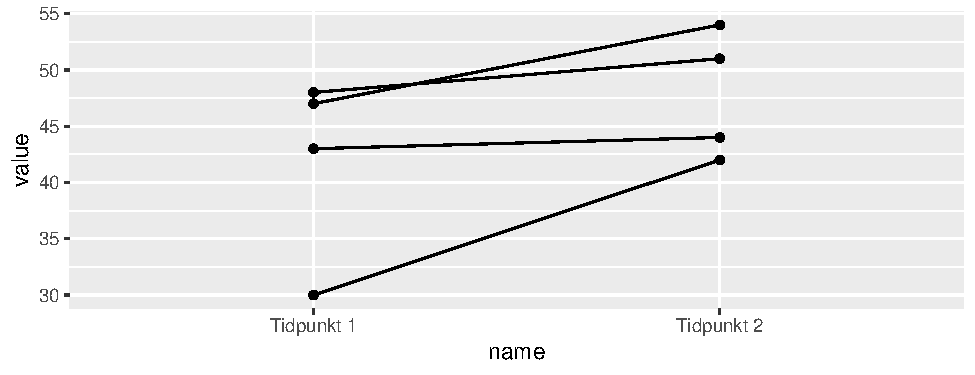
\includegraphics{R-anvisningar_files/figure-latex/unnamed-chunk-130-1} \end{center}

\begin{Shaded}
\begin{Highlighting}[]
\FunctionTok{mean}\NormalTok{(p\_values }\SpecialCharTok{\textless{}} \FloatTok{0.05}\NormalTok{)}
\end{Highlighting}
\end{Shaded}

\begin{verbatim}
## [1] 0.0497
\end{verbatim}

När slumptalen genereras från en normalfördelning med medelvärde 0 följer p-värdena en likformig fördelning. Ganska exakt 5 procent av simuleringarna ger ett p-värde under 5 procent. Detta är simuleringar i situationen att nollhypotesen är sann - sannolikheten att felaktigt förkasta på femprocentsnivån när nollhypotesen stämmer är alltså fem procent. Detta är alltså risken för falska positiva resultat.

\begin{Shaded}
\begin{Highlighting}[]
\NormalTok{p\_values\_when\_mean\_0 }\OtherTok{\textless{}{-}} \ControlFlowTok{function}\NormalTok{()\{}
\NormalTok{  x }\OtherTok{\textless{}{-}} \FunctionTok{rnorm}\NormalTok{(}\DecValTok{100}\NormalTok{, }\AttributeTok{mean =} \FloatTok{0.1}\NormalTok{)}
\NormalTok{  test }\OtherTok{\textless{}{-}} \FunctionTok{t.test}\NormalTok{(x, }\AttributeTok{mu =} \DecValTok{0}\NormalTok{)}
\NormalTok{  test}\SpecialCharTok{$}\NormalTok{p.value}
\NormalTok{\}}

\NormalTok{p\_values }\OtherTok{\textless{}{-}} \FunctionTok{replicate}\NormalTok{(}\DecValTok{10000}\NormalTok{, }\FunctionTok{p\_values\_when\_mean\_0}\NormalTok{())}

\NormalTok{dat }\OtherTok{\textless{}{-}} \FunctionTok{tibble}\NormalTok{(p\_values)}
\FunctionTok{ggplot}\NormalTok{(dat, }\FunctionTok{aes}\NormalTok{(p\_values)) }\SpecialCharTok{+}
  \FunctionTok{geom\_histogram}\NormalTok{(}\AttributeTok{breaks =} \FunctionTok{seq}\NormalTok{(}\DecValTok{0}\NormalTok{, }\DecValTok{1}\NormalTok{, }\FloatTok{0.05}\NormalTok{))}
\end{Highlighting}
\end{Shaded}

\begin{center}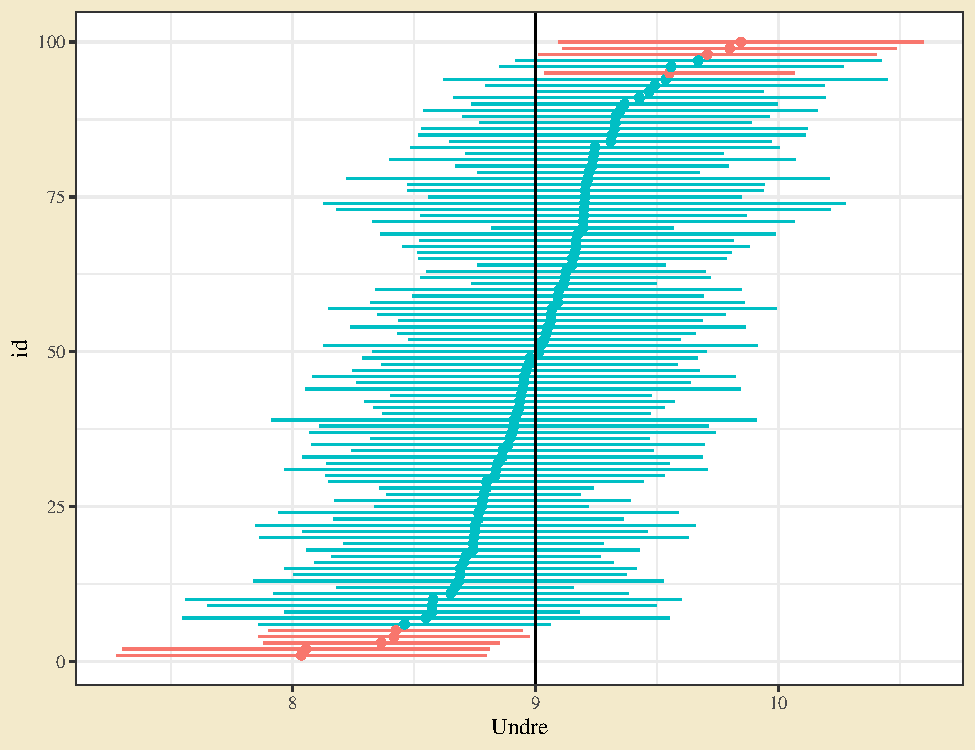
\includegraphics{R-anvisningar_files/figure-latex/unnamed-chunk-131-1} \end{center}

\begin{Shaded}
\begin{Highlighting}[]
\FunctionTok{mean}\NormalTok{(p\_values }\SpecialCharTok{\textless{}} \FloatTok{0.05}\NormalTok{)}
\end{Highlighting}
\end{Shaded}

\begin{verbatim}
## [1] 0.1705
\end{verbatim}

När slumptalen istället genereras från en normalfördelning med medelvärde 0.1 följer p-värdena en avtagande kurva men högst sannolikheter kring noll. Runt 16 procent av simuleringarna har givit p-värden under 0.05 - man har alltså en större chans att korrekt förkasta nollhypotesen när den inte stämmer. Notera att man ändå har ganska låg sannolikhet att förkasta nollhypotesen.
\end{hypothesis}

\begin{exercise}[Guldfiskgenetik]
En teori inom genetik förutsäger att tre fjärdedelar i en grupp guldfiskar ska ha genomskinliga fjäll. Observationer ger att nittio av hundra har genomskinliga fjäll. Genomför ett test för att se om den faktiska proportionen skiljer sig från 0.75.

(Fråga från Olsson, \emph{Biometri})
\end{exercise}

\begin{hypothesis}[Guldfiskgenetik]
Frågan kan hanteras med ett \(\chi^2\)-test, ett z-test eller ett binomialtest. Här ges exempel på det första. Nollhypotesen är att sannolikheten för genomskinliga fjäll är tre fjärdedelar. Notera att funktionen anges både med antalet (och andelen under nollhypotesen) med genomskinliga fjäll och antalet med färglagda fjäll.

\begin{Shaded}
\begin{Highlighting}[]
\FunctionTok{chisq.test}\NormalTok{(}\FunctionTok{c}\NormalTok{(}\DecValTok{90}\NormalTok{, }\DecValTok{10}\NormalTok{), }\AttributeTok{p =} \FunctionTok{c}\NormalTok{(}\FloatTok{0.75}\NormalTok{, }\FloatTok{0.25}\NormalTok{))}
\end{Highlighting}
\end{Shaded}

\begin{verbatim}
## 
##  Chi-squared test for given probabilities
## 
## data:  c(90, 10)
## X-squared = 12, df = 1, p-value = 0.000532
\end{verbatim}

Det låga p-värdet tyder på att den sanna sannolikheten för genomskinliga fjäll inte är 0.75.
\end{hypothesis}

\begin{exercise}[Mer guldfiskgenetik]
En konkurrerande teori inom genetik förutsäger att femton sextondelar (proportionen 0.9375) ska ha genomskinliga fjäll. Observationer ger att nittio av hundra har genomskinliga fjäll. Genomför ett test för att se om proportionen skiljer sig från 0.9375.
\end{exercise}

\begin{hypothesis}[Mer guldfiskgenetik]
Frågan kan hanteras med ett \(\chi^2\)-test. Nollhypotesen är att sannolikheten är genomskinliga fjäll är femton sextondelar.

\begin{Shaded}
\begin{Highlighting}[]
\FunctionTok{chisq.test}\NormalTok{(}\FunctionTok{c}\NormalTok{(}\DecValTok{90}\NormalTok{, }\DecValTok{10}\NormalTok{), }\AttributeTok{p =} \FunctionTok{c}\NormalTok{(}\DecValTok{15}\SpecialCharTok{/}\DecValTok{16}\NormalTok{, }\DecValTok{1}\SpecialCharTok{/}\DecValTok{16}\NormalTok{))}
\end{Highlighting}
\end{Shaded}

\begin{verbatim}
## 
##  Chi-squared test for given probabilities
## 
## data:  c(90, 10)
## X-squared = 2.4, df = 1, p-value = 0.1213
\end{verbatim}

Nollhypotesen att sannolikheten för genomskinliga fjäll är femton sextondelar, \(p = 15/16\), kan ej förkastas, eftersom testet ger ett p-värde över de vanliga signifikansnivåerna.
\end{hypothesis}

\begin{exercise}[Artobservationer]
Ekologisk data på populationsstorlekar kan samlas in genom att en observatör följer en rak slinga (en transekt) i ett naturområde och räknar antalet observerade individer. I en transektundersökning av storlom utförs 200 observationer med resultat nedan. Data finns tillgänglig bland kursdatan.

\begin{table}
\centering
\begin{tabular}[t]{rr}
\toprule
Antal observerade & n\\
\midrule
0 & 25\\
1 & 53\\
2 & 51\\
3 & 36\\
4 & 17\\
\addlinespace
5 & 18\\
\bottomrule
\end{tabular}
\end{table}

\emph{Observerade} anger antalet observerade individer och \emph{n} anger antalet transekter med det utfallet. Från tidigare studier förväntar man sig 1.7 observationer per transektgång. Genomför ett \emph{goodness-of-fit}-test för att undersöka om antalet observerade individer följer en poissonfördelning med \(\lambda = 1.7\).
\end{exercise}

\begin{hypothesis}[Artobservationer]
Ett goodness-of-fit-test kan genomföras genom att först beräkna det förväntade antalet observationer om nollhypotesen stämmer, det vill säga om antalet observerade individer följer en poissonfördelning med \(\lambda = 1.7\).
Förväntat antal beräknas genom att ta fram sannolikheterna för utfallet noll till 5 från poissonfördelning och multiplicera med 200.
För att sannolikheterna ska summera till 1 sätts sannolikheten att observera fem individer till ett minus summan av sannolikheten att få färre än 5.

\begin{Shaded}
\begin{Highlighting}[]
\NormalTok{prob\_poisson }\OtherTok{\textless{}{-}} \FunctionTok{dpois}\NormalTok{(}\AttributeTok{x =} \DecValTok{0}\SpecialCharTok{:}\DecValTok{5}\NormalTok{, }\AttributeTok{lambda =} \FloatTok{1.7}\NormalTok{)}
\NormalTok{prob\_poisson[}\DecValTok{6}\NormalTok{] }\OtherTok{\textless{}{-}} \DecValTok{1} \SpecialCharTok{{-}} \FunctionTok{sum}\NormalTok{(prob\_poisson[}\DecValTok{0}\SpecialCharTok{:}\DecValTok{5}\NormalTok{])}

\NormalTok{expected\_counts }\OtherTok{\textless{}{-}}\NormalTok{ prob\_poisson }\SpecialCharTok{*} \DecValTok{200}
\end{Highlighting}
\end{Shaded}

Datan kan illusteras med ett stapeldiagram. Stapeln ger faktiska observationer medan punkten ger det förväntade antalet under nollhypotesen.

\begin{Shaded}
\begin{Highlighting}[]
\NormalTok{dat }\OtherTok{\textless{}{-}} \FunctionTok{read\_csv}\NormalTok{(}\StringTok{"Data/Transektdata Storlom.csv"}\NormalTok{)}
\NormalTok{dat }\OtherTok{\textless{}{-}}\NormalTok{ dat }\SpecialCharTok{\%\textgreater{}\%} 
  \FunctionTok{count}\NormalTok{(}\StringTok{\textasciigrave{}}\AttributeTok{Antal observerade}\StringTok{\textasciigrave{}}\NormalTok{) }\SpecialCharTok{\%\textgreater{}\%} 
  \FunctionTok{mutate}\NormalTok{(}\StringTok{\textasciigrave{}}\AttributeTok{Sannolikheter enligt nollhypotes}\StringTok{\textasciigrave{}} \OtherTok{=}\NormalTok{ prob\_poisson,}
         \StringTok{\textasciigrave{}}\AttributeTok{Förväntat antal}\StringTok{\textasciigrave{}} \OtherTok{=}\NormalTok{ expected\_counts)}

\FunctionTok{ggplot}\NormalTok{(dat, }\FunctionTok{aes}\NormalTok{(}\StringTok{\textasciigrave{}}\AttributeTok{Antal observerade}\StringTok{\textasciigrave{}}\NormalTok{, n)) }\SpecialCharTok{+}
  \FunctionTok{geom\_bar}\NormalTok{(}\AttributeTok{stat =} \StringTok{"identity"}\NormalTok{, }\AttributeTok{width =} \FloatTok{0.5}\NormalTok{, }
           \AttributeTok{fill =} \StringTok{"white"}\NormalTok{, }\AttributeTok{color =} \StringTok{"black"}\NormalTok{) }\SpecialCharTok{+}
  \FunctionTok{geom\_point}\NormalTok{(}\FunctionTok{aes}\NormalTok{(}\AttributeTok{y =} \StringTok{\textasciigrave{}}\AttributeTok{Förväntat antal}\StringTok{\textasciigrave{}}\NormalTok{), }\AttributeTok{color =} \StringTok{"red"}\NormalTok{)}
\end{Highlighting}
\end{Shaded}

\begin{center}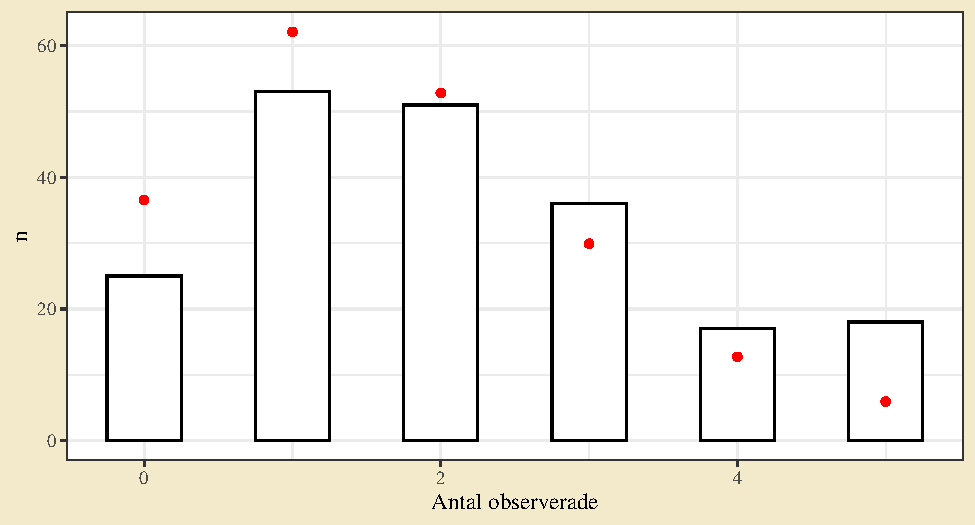
\includegraphics{R-anvisningar_files/figure-latex/unnamed-chunk-136-1} \end{center}

Observerade antal verkar inte perfekt följa nollhypotesens förväntade värden.

Ett formellt test genomförs som ett chi-två-test. Eftersom värdet på \(\lambda\) inte skattas från datan ges antalet frihetsgrader av antalet klasser minus ett. Testet genomförs i R med \texttt{chisq.test}.

\begin{Shaded}
\begin{Highlighting}[]
\FunctionTok{chisq.test}\NormalTok{(dat}\SpecialCharTok{$}\NormalTok{n, }\AttributeTok{p =}\NormalTok{ dat}\SpecialCharTok{$}\StringTok{\textasciigrave{}}\AttributeTok{Sannolikheter enligt nollhypotes}\StringTok{\textasciigrave{}}\NormalTok{)}
\end{Highlighting}
\end{Shaded}

\begin{verbatim}
## 
##  Chi-squared test for given probabilities
## 
## data:  dat$n
## X-squared = 32.347, df = 5, p-value = 5.072e-06
\end{verbatim}

Det låga p-värdet ger att man förkastar nollhypotesen. Det finns en statistiskt säkerställd skillnad mellan den observerade fördelningen och en poissonfördelning med \(\lambda = 1.7\).
\end{hypothesis}

\begin{exercise}[Simulering konfidensintervall]
Konfidensinterval konstrueras så att det sanna parametervärdet ingår i intervallet med en viss konfidensgrad (oftast 95 procent). Skriv en funktion som drar 10 slumptal från en normalfördelning med medelvärdet 9 och beräknar konfidensintervall. Upprepa funktionen 10000 gånger. Hur ofta täcker intervallet 9?

Notera att detta är en svårare uppgift.
\end{exercise}

\begin{hypothesis}[Simulering konfidensintervall]
Här konstrueras en funktion som drar 10 slumptal och beräknar ett konfidensintervall. Eftersom funktionen ger två värden (intervallets lägre och övre gräns) behövs lite mer hantering än i tidigare exempel (där de funktioner som använts givit ett utfallsvärde).

\begin{Shaded}
\begin{Highlighting}[]
\NormalTok{ci\_from\_ten }\OtherTok{\textless{}{-}} \ControlFlowTok{function}\NormalTok{()\{}
\NormalTok{  x }\OtherTok{\textless{}{-}} \FunctionTok{rnorm}\NormalTok{(}\DecValTok{10}\NormalTok{, }\AttributeTok{mean =} \DecValTok{9}\NormalTok{)}
\NormalTok{  test }\OtherTok{\textless{}{-}} \FunctionTok{t.test}\NormalTok{(x)}
\NormalTok{  test}\SpecialCharTok{$}\NormalTok{conf.int}
\NormalTok{\}}

\NormalTok{intervals }\OtherTok{\textless{}{-}} \FunctionTok{replicate}\NormalTok{(}\DecValTok{10000}\NormalTok{, }\FunctionTok{ci\_from\_ten}\NormalTok{())}
\NormalTok{intervals }\OtherTok{\textless{}{-}} \FunctionTok{t}\NormalTok{(intervals) }\CommentTok{\# Transponera till kolumner}
\NormalTok{intervals }\OtherTok{\textless{}{-}} \FunctionTok{as.data.frame}\NormalTok{(intervals)}
\FunctionTok{names}\NormalTok{(intervals) }\OtherTok{\textless{}{-}} \FunctionTok{c}\NormalTok{(}\StringTok{"Undre"}\NormalTok{, }\StringTok{"Övre"}\NormalTok{)}

\FunctionTok{mean}\NormalTok{(intervals}\SpecialCharTok{$}\NormalTok{Undre }\SpecialCharTok{\textgreater{}} \DecValTok{9}\NormalTok{)}
\end{Highlighting}
\end{Shaded}

\begin{verbatim}
## [1] 0.0266
\end{verbatim}

\begin{Shaded}
\begin{Highlighting}[]
\FunctionTok{mean}\NormalTok{(intervals}\SpecialCharTok{$}\NormalTok{Övre }\SpecialCharTok{\textless{}} \DecValTok{9}\NormalTok{)}
\end{Highlighting}
\end{Shaded}

\begin{verbatim}
## [1] 0.0241
\end{verbatim}

Värdet 9 ligger under den övre gränsen ungefär 2.5 procent av gångerna och över den undre gränsen ungefär 2.5 gångerna. Intervallet täcker alltså 9 ungefär 95 procent av gångerna.

En illustration med 100 simulerade fall.

\begin{Shaded}
\begin{Highlighting}[]
\NormalTok{intervals }\OtherTok{\textless{}{-}} \FunctionTok{replicate}\NormalTok{(}\DecValTok{100}\NormalTok{, }\FunctionTok{ci\_from\_ten}\NormalTok{())}
\NormalTok{intervals }\OtherTok{\textless{}{-}} \FunctionTok{t}\NormalTok{(intervals) }\CommentTok{\# Transponera till kolumner}
\NormalTok{intervals }\OtherTok{\textless{}{-}} \FunctionTok{as.data.frame}\NormalTok{(intervals)}
\FunctionTok{names}\NormalTok{(intervals) }\OtherTok{\textless{}{-}} \FunctionTok{c}\NormalTok{(}\StringTok{"Undre"}\NormalTok{, }\StringTok{"Övre"}\NormalTok{)}

\NormalTok{intervals }\SpecialCharTok{\%\textgreater{}\%} 
  \FunctionTok{arrange}\NormalTok{(Undre }\SpecialCharTok{+}\NormalTok{ Övre) }\SpecialCharTok{\%\textgreater{}\%} 
  \FunctionTok{mutate}\NormalTok{(}\AttributeTok{id =} \DecValTok{1}\SpecialCharTok{:}\FunctionTok{n}\NormalTok{(),}
\NormalTok{         Täcker}\AttributeTok{\_9 =}\NormalTok{ Undre }\SpecialCharTok{\textless{}} \DecValTok{9} \SpecialCharTok{\&}\NormalTok{ Övre }\SpecialCharTok{\textgreater{}} \DecValTok{9}\NormalTok{) }\SpecialCharTok{\%\textgreater{}\%} 
  \FunctionTok{ggplot}\NormalTok{(}\FunctionTok{aes}\NormalTok{(}\AttributeTok{x =}\NormalTok{ Undre, }\AttributeTok{xend =}\NormalTok{ Övre, }\AttributeTok{y =}\NormalTok{ id, }\AttributeTok{yend =}\NormalTok{ id, }\AttributeTok{col =}\NormalTok{ Täcker\_9)) }\SpecialCharTok{+}
  \FunctionTok{geom\_segment}\NormalTok{() }\SpecialCharTok{+}
  \FunctionTok{geom\_point}\NormalTok{(}\FunctionTok{aes}\NormalTok{(}\AttributeTok{x =}\NormalTok{ (Övre }\SpecialCharTok{+}\NormalTok{ Undre) }\SpecialCharTok{/} \DecValTok{2}\NormalTok{, id)) }\SpecialCharTok{+}
  \FunctionTok{geom\_vline}\NormalTok{(}\AttributeTok{xintercept =} \DecValTok{9}\NormalTok{) }\SpecialCharTok{+}
  \FunctionTok{theme}\NormalTok{(}\AttributeTok{legend.position =} \StringTok{"none"}\NormalTok{)}
\end{Highlighting}
\end{Shaded}

\begin{center}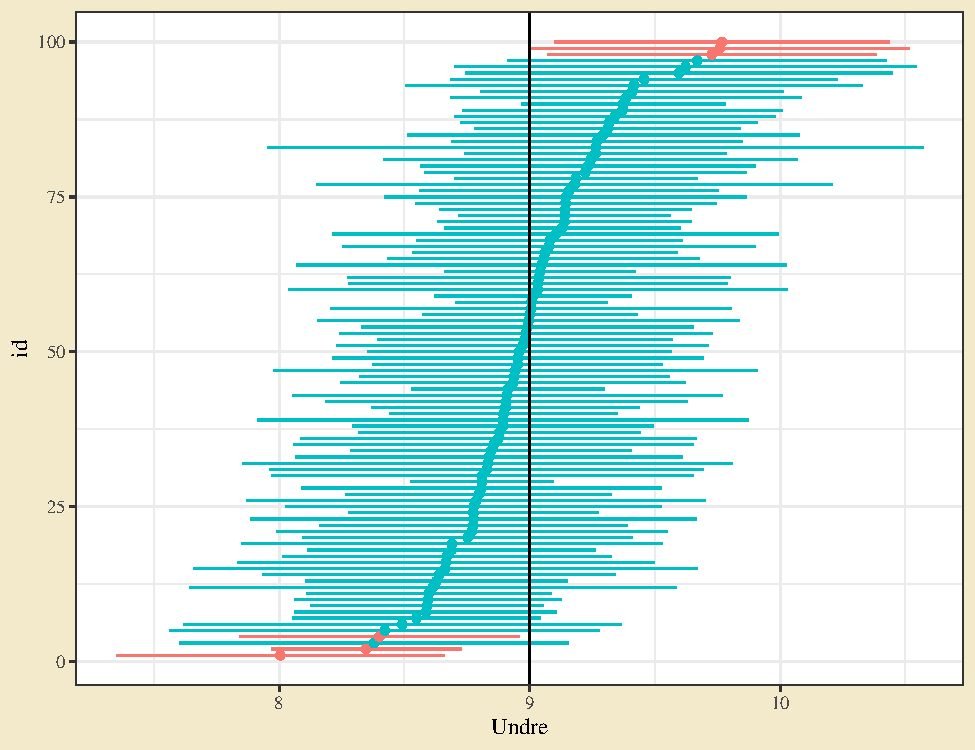
\includegraphics{R-anvisningar_files/figure-latex/unnamed-chunk-139-1} \end{center}

Varje streck motsvarar konfidensintervallet från en simulering. Intervallet väntas täcka 9 i 95 av hundra fall, men det kan förstås variera eftersom det beror på slumptalen.
\end{hypothesis}

\hypertarget{tvuxe5-stickprov}{%
\chapter{Två stickprov}\label{tvuxe5-stickprov}}

\hypertarget{normalfuxf6rdelad-data-eller-stora-stickprov-1}{%
\section{Normalfördelad data (eller stora stickprov)}\label{normalfuxf6rdelad-data-eller-stora-stickprov-1}}

t-test för två stickprov används för att jämföra två grupper och se om de har samma populationsmedelvärde i någon insamlad utfallsvariabel. Det finns två specifika fall: t-test för matchade stickprov, där det finns en parvis koppling mellan de två stickproven, t.ex. att de är mätningar på två syskon; och t-test för oberoende stickprov, där det saknas en sådan koppling mellan stickproven.

\hypertarget{t-test-fuxf6r-tvuxe5-matchade-stickprov}{%
\subsection{t-test för två matchade stickprov}\label{t-test-fuxf6r-tvuxe5-matchade-stickprov}}

Vid matchade stickprov kan varje observation i en behandlingsgrupp paras med en observation i den andra gruppen. Själva testet är ett t-test för \emph{ett} stickprov på differensserien beräknat från varje par. I R kan man antingen beräkna den differensserien eller använda \texttt{t.test}-funktionen med två dataserier och argumentet för parvisa observationer satt till sant, \texttt{paired\ =\ T}.
Som exempel ges följande data från en studie på äpple, där trädhöjd mätts före och efter en näringsbehandling.

\begin{Shaded}
\begin{Highlighting}[]
\NormalTok{dat }\OtherTok{\textless{}{-}} \FunctionTok{tibble}\NormalTok{(TrädID }\OtherTok{=} \DecValTok{1}\SpecialCharTok{:}\DecValTok{4}\NormalTok{, }
              \StringTok{\textasciigrave{}}\AttributeTok{Tidpunkt 1}\StringTok{\textasciigrave{}} \OtherTok{=} \FunctionTok{c}\NormalTok{(}\DecValTok{48}\NormalTok{, }\DecValTok{43}\NormalTok{, }\DecValTok{30}\NormalTok{, }\DecValTok{47}\NormalTok{), }
              \StringTok{\textasciigrave{}}\AttributeTok{Tidpunkt 2}\StringTok{\textasciigrave{}} \OtherTok{=} \FunctionTok{c}\NormalTok{(}\DecValTok{51}\NormalTok{, }\DecValTok{44}\NormalTok{, }\DecValTok{42}\NormalTok{, }\DecValTok{54}\NormalTok{))}
\NormalTok{dat}
\end{Highlighting}
\end{Shaded}

\begin{verbatim}
## # A tibble: 4 x 3
##   TrädID `Tidpunkt 1` `Tidpunkt 2`
##    <int>        <dbl>        <dbl>
## 1      1           48           51
## 2      2           43           44
## 3      3           30           42
## 4      4           47           54
\end{verbatim}

Datan kan illustreras med ett punktdiagram där en linje binder samman paret. För att enkelt skapa grafen i \texttt{ggplot2} kan man först omstrukturera datan till lång form genom \texttt{pivot\_longer}.

\begin{Shaded}
\begin{Highlighting}[]
\NormalTok{dat\_long }\OtherTok{\textless{}{-}}\NormalTok{ dat }\SpecialCharTok{\%\textgreater{}\%} \FunctionTok{pivot\_longer}\NormalTok{(}\SpecialCharTok{{-}}\NormalTok{TrädID)}
\NormalTok{dat\_long}
\end{Highlighting}
\end{Shaded}

\begin{verbatim}
## # A tibble: 8 x 3
##   TrädID name       value
##    <int> <chr>      <dbl>
## 1      1 Tidpunkt 1    48
## 2      1 Tidpunkt 2    51
## 3      2 Tidpunkt 1    43
## 4      2 Tidpunkt 2    44
## 5      3 Tidpunkt 1    30
## 6      3 Tidpunkt 2    42
## 7      4 Tidpunkt 1    47
## 8      4 Tidpunkt 2    54
\end{verbatim}

\begin{Shaded}
\begin{Highlighting}[]
\FunctionTok{ggplot}\NormalTok{(dat\_long, }\FunctionTok{aes}\NormalTok{(name, value, }\AttributeTok{group =}\NormalTok{ TrädID)) }\SpecialCharTok{+}
  \FunctionTok{geom\_point}\NormalTok{() }\SpecialCharTok{+}
  \FunctionTok{geom\_line}\NormalTok{()}
\end{Highlighting}
\end{Shaded}

\begin{center}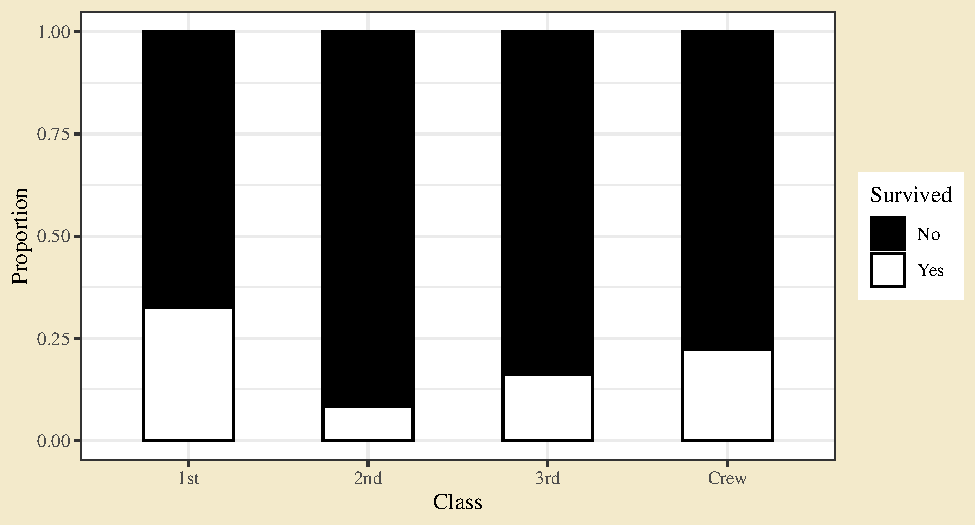
\includegraphics{R-anvisningar_files/figure-latex/unnamed-chunk-142-1} \end{center}

Testet för parade stickprov kan antingen utföras som ett enkelt t-test på differensserien

\begin{Shaded}
\begin{Highlighting}[]
\FunctionTok{t.test}\NormalTok{(dat}\SpecialCharTok{$}\StringTok{\textasciigrave{}}\AttributeTok{Tidpunkt 2}\StringTok{\textasciigrave{}} \SpecialCharTok{{-}}\NormalTok{ dat}\SpecialCharTok{$}\StringTok{\textasciigrave{}}\AttributeTok{Tidpunkt 1}\StringTok{\textasciigrave{}}\NormalTok{)}
\end{Highlighting}
\end{Shaded}

\begin{verbatim}
## 
##  One Sample t-test
## 
## data:  dat$`Tidpunkt 2` - dat$`Tidpunkt 1`
## t = 2.3681, df = 3, p-value = 0.09868
## alternative hypothesis: true mean is not equal to 0
## 95 percent confidence interval:
##  -1.977405 13.477405
## sample estimates:
## mean of x 
##      5.75
\end{verbatim}

eller som ett t-test för två stickprov där man särskilt anger att datan är parad

\begin{Shaded}
\begin{Highlighting}[]
\FunctionTok{t.test}\NormalTok{(dat}\SpecialCharTok{$}\StringTok{\textasciigrave{}}\AttributeTok{Tidpunkt 1}\StringTok{\textasciigrave{}}\NormalTok{, dat}\SpecialCharTok{$}\StringTok{\textasciigrave{}}\AttributeTok{Tidpunkt 2}\StringTok{\textasciigrave{}}\NormalTok{, }\AttributeTok{paired =}\NormalTok{ T)}
\end{Highlighting}
\end{Shaded}

\begin{verbatim}
## 
##  Paired t-test
## 
## data:  dat$`Tidpunkt 1` and dat$`Tidpunkt 2`
## t = -2.3681, df = 3, p-value = 0.09868
## alternative hypothesis: true difference in means is not equal to 0
## 95 percent confidence interval:
##  -13.477405   1.977405
## sample estimates:
## mean of the differences 
##                   -5.75
\end{verbatim}

För bägge alternativen måste datan vara ordnad så att de två vektorerna matchar varandra parvis. Notera att ordningen på vektorerna påverkar konfidensintervall men inte p-värdet (i fallet med en tvåsidig mothypotes). Här är det naturligt att ta den andra mätningen först eftersom konfidensintervallet då blir ett intervall för medelvärdesökningen efter behandling. Ett p-värde på \(0.0987\) ger att man inte förkastar vid en signifikansnivå på fem procent.

\hypertarget{t-test-fuxf6r-tvuxe5-oberoende-stickprov}{%
\subsection{t-test för två oberoende stickprov}\label{t-test-fuxf6r-tvuxe5-oberoende-stickprov}}

Ett t-test för två oberoende stickprov testar om två populationsmedelvärden är lika. Ta som exempel följande data på jordgubbsskörd vid två olika näringsbehandlingar (A och B). Här är stickprov inte matchade - det finns ingen direkt koppling mellan en observation i den ena behandlingsgruppen till någon observation i den andra.

\begin{Shaded}
\begin{Highlighting}[]
\NormalTok{dat }\OtherTok{\textless{}{-}} \FunctionTok{tibble}\NormalTok{(}\AttributeTok{Behandling =} \FunctionTok{c}\NormalTok{(}\StringTok{"A"}\NormalTok{, }\StringTok{"A"}\NormalTok{, }\StringTok{"A"}\NormalTok{, }\StringTok{"A"}\NormalTok{, }\StringTok{"B"}\NormalTok{, }\StringTok{"B"}\NormalTok{, }\StringTok{"B"}\NormalTok{, }\StringTok{"B"}\NormalTok{),}
              \AttributeTok{Vikt =} \FunctionTok{c}\NormalTok{(}\DecValTok{40}\NormalTok{, }\FloatTok{48.2}\NormalTok{, }\FloatTok{39.2}\NormalTok{, }\FloatTok{47.9}\NormalTok{, }\FloatTok{57.5}\NormalTok{, }\FloatTok{61.5}\NormalTok{, }\DecValTok{58}\NormalTok{, }\FloatTok{66.5}\NormalTok{))}
\FunctionTok{kable}\NormalTok{(dat)}
\end{Highlighting}
\end{Shaded}

\begin{table}
\centering
\begin{tabular}[t]{lr}
\toprule
Behandling & Vikt\\
\midrule
A & 40.0\\
A & 48.2\\
A & 39.2\\
A & 47.9\\
B & 57.5\\
\addlinespace
B & 61.5\\
B & 58.0\\
B & 66.5\\
\bottomrule
\end{tabular}
\end{table}

Datan kan illustreras med ett enkelt punktdiagram. I ett publiceringssammanhang hade det kanske presenterats med ett stapeldiagram med felstaplar.

\begin{Shaded}
\begin{Highlighting}[]
\NormalTok{g1 }\OtherTok{\textless{}{-}} \FunctionTok{ggplot}\NormalTok{(dat, }\FunctionTok{aes}\NormalTok{(Behandling, Vikt)) }\SpecialCharTok{+}
  \FunctionTok{geom\_point}\NormalTok{()}

\NormalTok{g2 }\OtherTok{\textless{}{-}}\NormalTok{ dat }\SpecialCharTok{\%\textgreater{}\%} 
  \FunctionTok{group\_by}\NormalTok{(Behandling) }\SpecialCharTok{\%\textgreater{}\%} 
  \FunctionTok{summarise}\NormalTok{(}\AttributeTok{m =} \FunctionTok{mean}\NormalTok{(Vikt), }\AttributeTok{s =} \FunctionTok{sd}\NormalTok{(Vikt)) }\SpecialCharTok{\%\textgreater{}\%} 
  \FunctionTok{ggplot}\NormalTok{(}\FunctionTok{aes}\NormalTok{(Behandling, m)) }\SpecialCharTok{+}
  \FunctionTok{geom\_bar}\NormalTok{(}\AttributeTok{stat =} \StringTok{"identity"}\NormalTok{, }\AttributeTok{fill =} \StringTok{"grey80"}\NormalTok{, }\AttributeTok{width =} \FloatTok{0.3}\NormalTok{) }\SpecialCharTok{+}
  \FunctionTok{geom\_errorbar}\NormalTok{(}\FunctionTok{aes}\NormalTok{(}\AttributeTok{ymin =}\NormalTok{ m }\SpecialCharTok{{-}}\NormalTok{ s, }\AttributeTok{ymax =}\NormalTok{ m }\SpecialCharTok{+}\NormalTok{ s), }\AttributeTok{width =} \FloatTok{0.1}\NormalTok{)}

\FunctionTok{library}\NormalTok{(patchwork)}
\NormalTok{g1 }\SpecialCharTok{+}\NormalTok{ g2}
\end{Highlighting}
\end{Shaded}

\begin{center}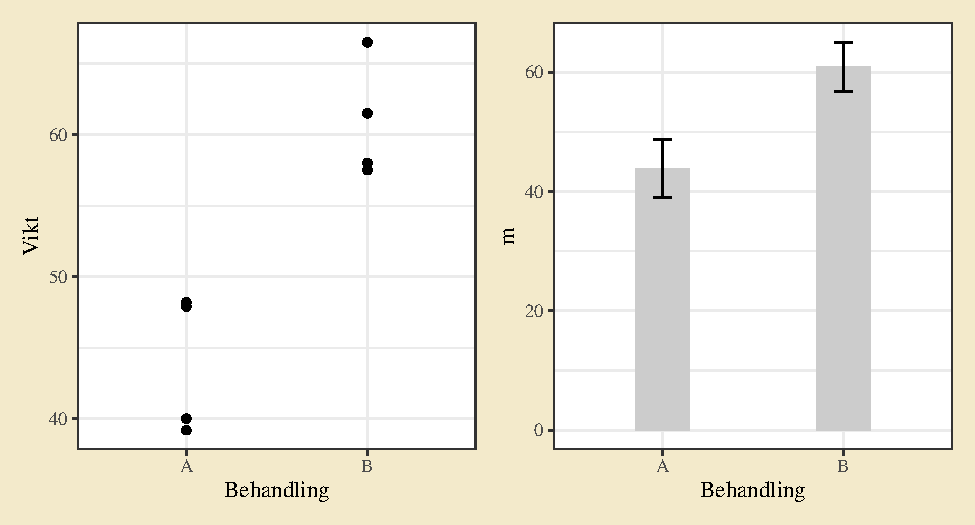
\includegraphics{R-anvisningar_files/figure-latex/unnamed-chunk-146-1} \end{center}

Ett t-test för två oberoende stickprov har nollhypotesen att grupperna har samma populationsmedelvärde och alternativhypotesen att populationsmedelvärdena är skilda (för det tvåsidiga fallet):

\[\mu_1 = \mu_2 \qquad \mu_1 \neq \mu_2.\]

Testet kan utföras i R genom funktionen \texttt{t.test}. Data kan antingen anges som en formel med dess data \texttt{Vikt\ \textasciitilde{}\ Behandling,\ data\ =\ dat} (vilket man kan läsa som \emph{vikt uppdelat efter behandling}) eller som två skilda vektorer. Det förra alternativet är oftast enklare om man har datan på lång form - med en kolumn som anger grupp (i exemplet \emph{Behandling}) och en kolumn som anger utfallsvärdet (i exemplet \emph{Vikt}).

\begin{Shaded}
\begin{Highlighting}[]
\CommentTok{\# Formelskrivning}
\FunctionTok{t.test}\NormalTok{(Vikt }\SpecialCharTok{\textasciitilde{}}\NormalTok{ Behandling, }\AttributeTok{data =}\NormalTok{ dat, }\AttributeTok{var.equal =}\NormalTok{ T)}
\end{Highlighting}
\end{Shaded}

\begin{verbatim}
## 
##  Two Sample t-test
## 
## data:  Vikt by Behandling
## t = -5.3157, df = 6, p-value = 0.001803
## alternative hypothesis: true difference in means between group A and group B is not equal to 0
## 95 percent confidence interval:
##  -24.898417  -9.201583
## sample estimates:
## mean in group A mean in group B 
##          43.825          60.875
\end{verbatim}

\begin{Shaded}
\begin{Highlighting}[]
\CommentTok{\# Två separata vektorer}
\DocumentationTok{\#\# Filtrera ut data där behandling är A}
\NormalTok{Vikt\_A }\OtherTok{\textless{}{-}}\NormalTok{ dat}\SpecialCharTok{$}\NormalTok{Vikt[dat}\SpecialCharTok{$}\NormalTok{Behandling }\SpecialCharTok{==} \StringTok{"A"}\NormalTok{]}

\DocumentationTok{\#\# Filtrera ut data där behandling är B}
\NormalTok{Vikt\_B }\OtherTok{\textless{}{-}}\NormalTok{ dat}\SpecialCharTok{$}\NormalTok{Vikt[dat}\SpecialCharTok{$}\NormalTok{Behandling }\SpecialCharTok{==} \StringTok{"B"}\NormalTok{]}

\FunctionTok{t.test}\NormalTok{(Vikt\_A, Vikt\_B, }\AttributeTok{var.equal =}\NormalTok{ T)}
\end{Highlighting}
\end{Shaded}

\begin{verbatim}
## 
##  Two Sample t-test
## 
## data:  Vikt_A and Vikt_B
## t = -5.3157, df = 6, p-value = 0.001803
## alternative hypothesis: true difference in means is not equal to 0
## 95 percent confidence interval:
##  -24.898417  -9.201583
## sample estimates:
## mean of x mean of y 
##    43.825    60.875
\end{verbatim}

Argumentet \texttt{var.equal\ =\ T} används för att beräkna testet där gruppernas varianser antas vara lika. Grundinställningen är testet där varianser inte antas vara lika, så \texttt{t.test(Vikt\ \textasciitilde{}\ Behandling,\ data\ =\ dat)} ger ett lite annat resultat.
Testet ger ett p-värde på \(0.0018\), vilket leder till att nollhypotesen förkastas på enprocentsnivån. Detta tyder på att det finns en viktskillnad mellan behandlingarna. Utskriften ger också ett 95-procentigt konfidensintervall på \((-24.898, -9.202)\). Tolkningen är att skillnaden mellan populationsmedelvärden ligger i intervallet med 95 procents konfidens. Notera att värdet noll inte ligger i intervallet.

\hypertarget{binuxe4r-data.-proportioner-1}{%
\section{Binär data. Proportioner}\label{binuxe4r-data.-proportioner-1}}

Om man vill jämföra två proportioner kan man använda z-testet för två stickprov. Säg till exempel att man utvecklar den tidigare studien, som gav 17 av 50 infekterade plantor, till att undersöka ytterligare en sort och att den sorten har 26 infekterade plantor av en total på 60. Testets hypotesen är i det tvåsidiga fallet

\[H_0: p_1 = p_2 \qquad H_1: p_1 \neq p_2.\]

I R kan testet genomföras med \texttt{prop.test}-funktionen. Funktionens första argument är antalen infekterade, som en vektor med två värden, och dess andra argument är totalerna. Likt testet med ett stickprov finns en möjlighet att göra en kontinuitetskorrektion med \texttt{correct}-argumentet.

\begin{Shaded}
\begin{Highlighting}[]
\FunctionTok{prop.test}\NormalTok{(}\FunctionTok{c}\NormalTok{(}\DecValTok{17}\NormalTok{, }\DecValTok{26}\NormalTok{), }\FunctionTok{c}\NormalTok{(}\DecValTok{50}\NormalTok{, }\DecValTok{60}\NormalTok{), }\AttributeTok{correct =}\NormalTok{ F)}
\end{Highlighting}
\end{Shaded}

\begin{verbatim}
## 
##  2-sample test for equality of proportions without continuity
##  correction
## 
## data:  c(17, 26) out of c(50, 60)
## X-squared = 0.9978, df = 1, p-value = 0.3178
## alternative hypothesis: two.sided
## 95 percent confidence interval:
##  -0.27488771  0.08822105
## sample estimates:
##    prop 1    prop 2 
## 0.3400000 0.4333333
\end{verbatim}

Notera att funktionen inte ger ett z-värde utan ett \(\chi^2\)-värde (utskrivet \texttt{X-squared}). Det beror på att funktionen beräknar z-testet som ett likvärdigt \(\chi^2\)-test. Det z-värde man får om man genomför testet som ett z-test är detsamma som roten ur utskriftens \(\chi^2\)-värde.
Testet ger ett högt p-värde vilket innebär att nollhypotesen inte förkastas.

\hypertarget{nominal-eller-ordinal-data.-korstabeller}{%
\section{Nominal eller ordinal data. Korstabeller}\label{nominal-eller-ordinal-data.-korstabeller}}

Data med två insamlade variabler per observerad enhet kan presenteras med en korstabell. Ta som (ett något deppigt) exempel överlevandsdata från Titanic. Datan finns tillgänglig i R som \texttt{Titanic} och man kan konstruera en korstabell med \texttt{pivot\_wider}. I detta fall ges överlevnad filtrerad på vuxna män, uppdelat efter klass.

\begin{Shaded}
\begin{Highlighting}[]
\NormalTok{dat }\OtherTok{\textless{}{-}}\NormalTok{ Titanic }\SpecialCharTok{\%\textgreater{}\%} 
  \FunctionTok{as\_tibble}\NormalTok{() }\SpecialCharTok{\%\textgreater{}\%} 
  \FunctionTok{filter}\NormalTok{(Age }\SpecialCharTok{==} \StringTok{"Adult"}\NormalTok{, Sex }\SpecialCharTok{==} \StringTok{"Male"}\NormalTok{)}
\FunctionTok{kable}\NormalTok{(dat)}
\end{Highlighting}
\end{Shaded}

\begin{table}
\centering
\begin{tabular}[t]{llllr}
\toprule
Class & Sex & Age & Survived & n\\
\midrule
1st & Male & Adult & No & 118\\
2nd & Male & Adult & No & 154\\
3rd & Male & Adult & No & 387\\
Crew & Male & Adult & No & 670\\
1st & Male & Adult & Yes & 57\\
\addlinespace
2nd & Male & Adult & Yes & 14\\
3rd & Male & Adult & Yes & 75\\
Crew & Male & Adult & Yes & 192\\
\bottomrule
\end{tabular}
\end{table}

En korstabell kan konstrueras med \texttt{pivot\_wider}.

\begin{Shaded}
\begin{Highlighting}[]
\NormalTok{dat\_wide }\OtherTok{\textless{}{-}}\NormalTok{ dat }\SpecialCharTok{\%\textgreater{}\%} 
  \FunctionTok{pivot\_wider}\NormalTok{(}\AttributeTok{names\_from =}\NormalTok{ Survived, }\AttributeTok{values\_from =}\NormalTok{ n)}
\end{Highlighting}
\end{Shaded}

Datan tyder på att överlevnad är beroende av klass - en tredjedel av förstaklass överlever, men en sjättedel av tredjeklass överlever. En illustration kan göras genom ett stapeldiagram.

\begin{Shaded}
\begin{Highlighting}[]
\FunctionTok{ggplot}\NormalTok{(dat, }\FunctionTok{aes}\NormalTok{(Class, n, }\AttributeTok{fill =}\NormalTok{ Survived)) }\SpecialCharTok{+}
  \FunctionTok{geom\_bar}\NormalTok{(}\AttributeTok{stat =} \StringTok{"identity"}\NormalTok{, }\AttributeTok{position =} \FunctionTok{position\_fill}\NormalTok{(), }
           \AttributeTok{color =} \StringTok{"black"}\NormalTok{, }\AttributeTok{width =} \FloatTok{0.5}\NormalTok{) }\SpecialCharTok{+}
  \FunctionTok{scale\_fill\_manual}\NormalTok{(}\AttributeTok{values =} \FunctionTok{c}\NormalTok{(}\StringTok{"black"}\NormalTok{, }\StringTok{"white"}\NormalTok{)) }\SpecialCharTok{+}
  \FunctionTok{ylab}\NormalTok{(}\StringTok{"Proportion"}\NormalTok{)}
\end{Highlighting}
\end{Shaded}

\begin{center}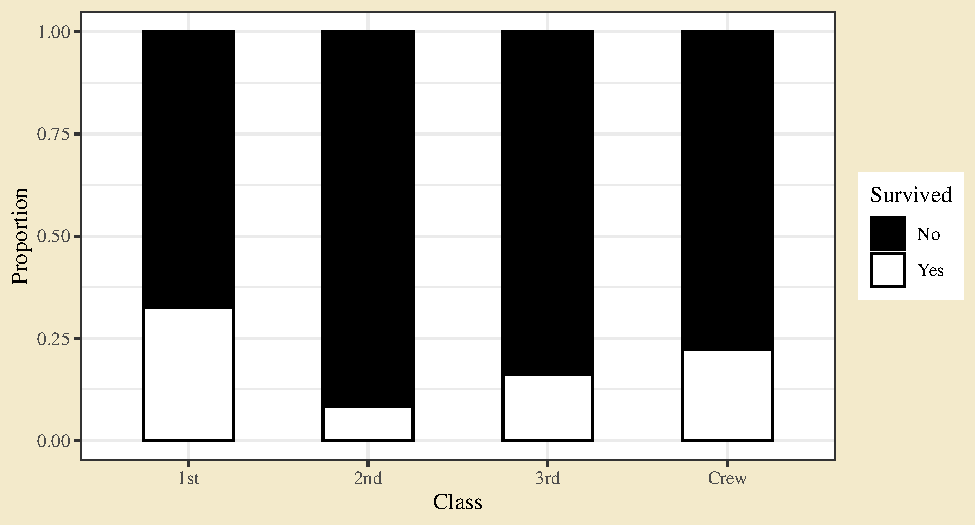
\includegraphics{R-anvisningar_files/figure-latex/unnamed-chunk-151-1} \end{center}

Argumentet \texttt{position} i \texttt{geom\_bar} används för att skapa proportionella staplar.

Ett \(\chi^2\)-test på en korstabell har nollhypotesen att det inte finns något samband mellan variabeln för rader och variabeln för kolumner. Antal frihetsgrader ges av antal rader minus ett gånger antal kolumner minus ett. Testet kan enkelt göras med \texttt{chisq.test}. Som ingångsvärde kan man plocka ut kolumnerna med numeriska värden genom hakparenteser.

\begin{Shaded}
\begin{Highlighting}[]
\NormalTok{dat\_wide[, }\DecValTok{4}\SpecialCharTok{:}\DecValTok{5}\NormalTok{] }\CommentTok{\# De två numeriska kolumnerna}
\end{Highlighting}
\end{Shaded}

\begin{verbatim}
## # A tibble: 4 x 2
##      No   Yes
##   <dbl> <dbl>
## 1   118    57
## 2   154    14
## 3   387    75
## 4   670   192
\end{verbatim}

\begin{Shaded}
\begin{Highlighting}[]
\FunctionTok{chisq.test}\NormalTok{(dat\_wide[, }\DecValTok{4}\SpecialCharTok{:}\DecValTok{5}\NormalTok{])}
\end{Highlighting}
\end{Shaded}

\begin{verbatim}
## 
##  Pearson's Chi-squared test
## 
## data:  dat_wide[, 4:5]
## X-squared = 37.988, df = 3, p-value = 2.843e-08
\end{verbatim}

Utskriften ger teststorheten, antal frihetsgrader, och p-värdet. I det här fallet är p-värdet mycket litet (skrivning med \texttt{e} ska läsas som \(2.843e-8 = 2.843 \cdot 10^{-8} = 0.00000002843\)) och slutsatsen blir att nollhypotesen förkastas - det finns ett samband mellan klass och överlevnad. Antalet frihetsgrader ges av antalet rader minus ett gånger antalet kolumner minus ett (här \((4-1) \cdot (2-1) = 3\)).

\(\chi^2\)-test är ett asymptotiskt test - dess egenskaper är beroende av \emph{stora} stickprov. Som gräns för storleken används ofta att samtliga förväntade antal ska vara större än 5. Funktionen ger en varning om förväntade värden är små. En möjlig lösning i sådana fall är att slå ihop klasser.

\begin{Shaded}
\begin{Highlighting}[]
\NormalTok{test\_result }\OtherTok{\textless{}{-}} \FunctionTok{chisq.test}\NormalTok{(dat\_wide[, }\DecValTok{4}\SpecialCharTok{:}\DecValTok{5}\NormalTok{])}
\NormalTok{test\_result}\SpecialCharTok{$}\NormalTok{expected }\CommentTok{\# Samtliga förväntade värden över 5}
\end{Highlighting}
\end{Shaded}

\begin{verbatim}
##            No       Yes
## [1,] 139.5171  35.48290
## [2,] 133.9364  34.06359
## [3,] 368.3251  93.67487
## [4,] 687.2214 174.77864
\end{verbatim}

Om detta krav inte är uppfyllt skriver funktionen ut en varning.

\begin{Shaded}
\begin{Highlighting}[]
\NormalTok{dat }\OtherTok{\textless{}{-}} \FunctionTok{matrix}\NormalTok{(}\FunctionTok{c}\NormalTok{(}\DecValTok{4}\NormalTok{,}\DecValTok{2}\NormalTok{,}\DecValTok{5}\NormalTok{,}\DecValTok{1}\NormalTok{), }\DecValTok{2}\NormalTok{)}
\NormalTok{test\_result }\OtherTok{\textless{}{-}} \FunctionTok{chisq.test}\NormalTok{(dat)}
\NormalTok{test\_result}\SpecialCharTok{$}\NormalTok{expected}
\end{Highlighting}
\end{Shaded}

\begin{verbatim}
##      [,1] [,2]
## [1,]  4.5  4.5
## [2,]  1.5  1.5
\end{verbatim}

\hypertarget{uxf6vningar-3}{%
\section{Övningar}\label{uxf6vningar-3}}

\begin{exercise}[Lök]
Åtta monoglukosidmätningar på lök samlas in från fyra konventionella och fyra ekologiska ordlare.

\begin{table}
\centering
\begin{tabular}[t]{lr}
\toprule
Odlingstyp & Monoglukosid\\
\midrule
Ekologisk & 135.7\\
Ekologisk & 186.7\\
Ekologisk & 182.0\\
Ekologisk & 180.5\\
Konventionell & 138.9\\
\addlinespace
Konventionell & 155.1\\
Konventionell & 126.3\\
Konventionell & 120.1\\
\bottomrule
\end{tabular}
\end{table}

a. Genomför ett hypotestest för att se om det finns en medelvärdesskillnad mellan odlingstyperna.

b. Beräkna ett 95-procentigt konfidensintervall för skillnaden i medelvärde.
\end{exercise}

\begin{hypothesis}[Lök]
Datan kan importeras från excelfilen med uppgiftsdata. En lämplig graf kan skapas genom att pivotera till långform och plotta med \texttt{ggplot}.

\begin{Shaded}
\begin{Highlighting}[]
\NormalTok{dat }\OtherTok{\textless{}{-}}\NormalTok{ readxl}\SpecialCharTok{::}\FunctionTok{read\_excel}\NormalTok{(}\StringTok{"Data/Uppgiftsdata.xlsx"}\NormalTok{, }\AttributeTok{sheet =} \StringTok{"Lökfärg"}\NormalTok{)}

\NormalTok{dat }\SpecialCharTok{\%\textgreater{}\%} 
  \FunctionTok{pivot\_longer}\NormalTok{(}\SpecialCharTok{{-}}\NormalTok{Odlare, }\AttributeTok{names\_to =} \StringTok{"Odlingstyp"}\NormalTok{, }
               \AttributeTok{values\_to =} \StringTok{"Monoglukosid"}\NormalTok{) }\SpecialCharTok{\%\textgreater{}\%} 
  \FunctionTok{ggplot}\NormalTok{(}\FunctionTok{aes}\NormalTok{(Odlingstyp, Monoglukosid)) }\SpecialCharTok{+}
  \FunctionTok{geom\_point}\NormalTok{()}
\end{Highlighting}
\end{Shaded}

\begin{center}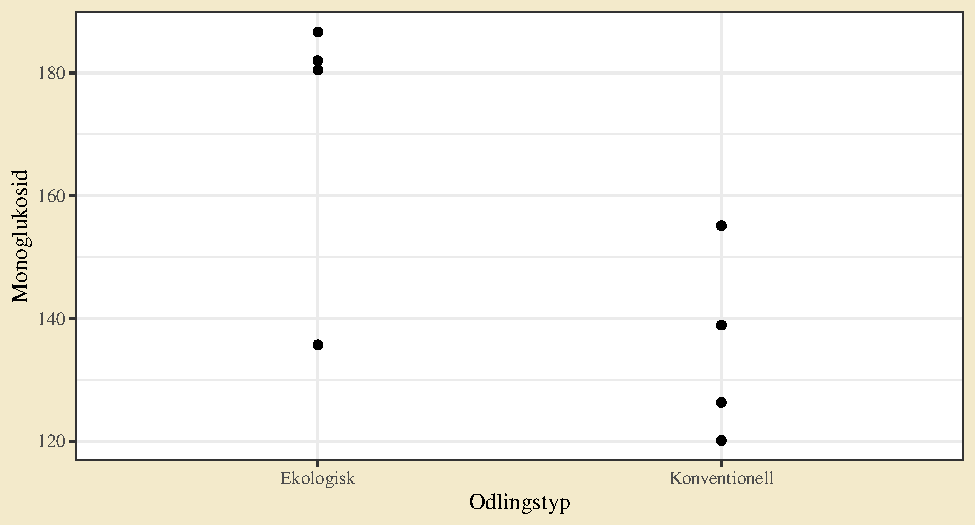
\includegraphics{R-anvisningar_files/figure-latex/unnamed-chunk-156-1} \end{center}

a. Eftersom det inte finns någon koppling mellan odlare är ett t-test för två oberoende stickprov ett lämpligt test. Testet kan genomföras med eller utan ett antagande om lika varianser inom grupperna.

\begin{Shaded}
\begin{Highlighting}[]
\FunctionTok{t.test}\NormalTok{(dat}\SpecialCharTok{$}\NormalTok{Konventionell, dat}\SpecialCharTok{$}\NormalTok{Ekologisk, }\AttributeTok{var.equal =}\NormalTok{ T)}
\end{Highlighting}
\end{Shaded}

\begin{verbatim}
## 
##  Two Sample t-test
## 
## data:  dat$Konventionell and dat$Ekologisk
## t = -2.5436, df = 6, p-value = 0.04387
## alternative hypothesis: true difference in means is not equal to 0
## 95 percent confidence interval:
##  -70.877089  -1.372911
## sample estimates:
## mean of x mean of y 
##   135.100   171.225
\end{verbatim}

\begin{Shaded}
\begin{Highlighting}[]
\FunctionTok{t.test}\NormalTok{(dat}\SpecialCharTok{$}\NormalTok{Konventionell, dat}\SpecialCharTok{$}\NormalTok{Ekologisk, }\AttributeTok{var.equal =}\NormalTok{ F)}
\end{Highlighting}
\end{Shaded}

\begin{verbatim}
## 
##  Welch Two Sample t-test
## 
## data:  dat$Konventionell and dat$Ekologisk
## t = -2.5436, df = 5.145, p-value = 0.05033
## alternative hypothesis: true difference in means is not equal to 0
## 95 percent confidence interval:
##  -72.32625466   0.07625466
## sample estimates:
## mean of x mean of y 
##   135.100   171.225
\end{verbatim}

Hypotestestet (ett t-test för två oberoende stickprov) ger ett p-värde på \(0.0439\) eller \(0.0503\), beroende på om varianser inom grupperna antas lika eller ej.

Om man har fler än två grupper kan man vilja göra parvisa t-test - alltså ett t-test för varje par av grupper.
Ett exempel på funktionen \texttt{pairwise.t.test} ges nedan. Funktionen bygger på att datan är i \emph{lång} form, med en kolumn som anger det numeriska utfallet och en kolumn som anger behandlingen.

\begin{Shaded}
\begin{Highlighting}[]
\NormalTok{dat\_long }\OtherTok{\textless{}{-}}\NormalTok{ dat }\SpecialCharTok{\%\textgreater{}\%} 
  \FunctionTok{pivot\_longer}\NormalTok{(}\SpecialCharTok{{-}}\NormalTok{Odlare, }\AttributeTok{names\_to =} \StringTok{"Odlingstyp"}\NormalTok{, }
               \AttributeTok{values\_to =} \StringTok{"Monoglukosid"}\NormalTok{)}

\FunctionTok{kable}\NormalTok{(dat\_long)}
\end{Highlighting}
\end{Shaded}

\begin{table}
\centering
\begin{tabular}[t]{rlr}
\toprule
Odlare & Odlingstyp & Monoglukosid\\
\midrule
1 & Konventionell & 138.9\\
1 & Ekologisk & 135.7\\
2 & Konventionell & 155.1\\
2 & Ekologisk & 186.7\\
3 & Konventionell & 126.3\\
\addlinespace
3 & Ekologisk & 182.0\\
4 & Konventionell & 120.1\\
4 & Ekologisk & 180.5\\
\bottomrule
\end{tabular}
\end{table}

\begin{Shaded}
\begin{Highlighting}[]
\FunctionTok{pairwise.t.test}\NormalTok{(dat\_long}\SpecialCharTok{$}\NormalTok{Monoglukosid, dat\_long}\SpecialCharTok{$}\NormalTok{Odlingstyp,}
                \AttributeTok{p.adjust.method =} \StringTok{"none"}\NormalTok{, }\AttributeTok{pool.sd =}\NormalTok{ F)}
\end{Highlighting}
\end{Shaded}

\begin{verbatim}
## 
##  Pairwise comparisons using t tests with non-pooled SD 
## 
## data:  dat_long$Monoglukosid and dat_long$Odlingstyp 
## 
##               Ekologisk
## Konventionell 0.05     
## 
## P value adjustment method: none
\end{verbatim}

b. Om varianser antas lika ges ett 95-procentigt konfidensintervall av \((-70.9, -1.4)\). Notera att ett 95-procentigt intervall inte täcker noll, vilket är i linje med att p-värdet är mindre än 5 procent.
\end{hypothesis}

\begin{exercise}[Ekorrar]
I en undersökning av hur den europeiska ekorren (Sciurus vulgaris) förändras i vikt under övervintring mäts 7 slumpmässigt valda ekorrar före och 5 slumpmässigt valda ekorrar efter övervintring.
Resultaten ges av tabell.

\begin{table}
\centering
\begin{tabular}[t]{lr}
\toprule
Tidpunkt & Vikt\\
\midrule
Före & 537\\
Före & 597\\
Före & 445\\
Före & 556\\
Före & 585\\
\addlinespace
Före & 542\\
Före & 415\\
Efter & 302\\
Efter & 326\\
Efter & 377\\
\addlinespace
Efter & 469\\
Efter & 417\\
\bottomrule
\end{tabular}
\end{table}

Medelvärde och standardavvikelse per grupp ges av följande.

\begin{table}
\centering
\begin{tabular}[t]{lrr}
\toprule
Tidpunkt & Medelvikt & Standardavvikelse\\
\midrule
Efter & 378.2000 & 67.6070\\
Före & 525.2857 & 69.1344\\
\bottomrule
\end{tabular}
\end{table}

Antag normalfördelad data och lika populationsvarianser i de bägge grupperna.

a. Konstruera ett 95-procentigt konfidensintervall för vikten före övervintring.
b. Gör ett hypotestest för att se om det är någon skillnad i vikt före och efter vintern. Använd signifikansnivån 5\%.
c. Ett problem med att mäta skilda individer före och efter övervintring är att det kan finnas en stor skillnad i vikt mellan ekorrar. Kan man lägga upp försöket på ett sätt som reducerar det problemet?

(Detta är en tentamensuppgift från 2019.)
\end{exercise}

\begin{hypothesis}[Ekorrar]
Data läses in från kursdatan, fliken \emph{Ekorrar}.

\begin{Shaded}
\begin{Highlighting}[]
\NormalTok{dat }\OtherTok{\textless{}{-}} \FunctionTok{read\_excel}\NormalTok{(}\StringTok{"Data/Uppgiftsdata.xlsx"}\NormalTok{, }\AttributeTok{sheet =} \StringTok{"Ekorrar"}\NormalTok{)}
\end{Highlighting}
\end{Shaded}

En illustration kan skapas som en punktdiagram med tidpunkt på ena axeln och vikt på den andra. Notera i det steget att det inte finns några lika vikter, och därmed inga överlappande punkter.

\begin{Shaded}
\begin{Highlighting}[]
\FunctionTok{ggplot}\NormalTok{(dat, }\FunctionTok{aes}\NormalTok{(Vikt, Tidpunkt)) }\SpecialCharTok{+} \FunctionTok{geom\_point}\NormalTok{()}
\end{Highlighting}
\end{Shaded}

\begin{center}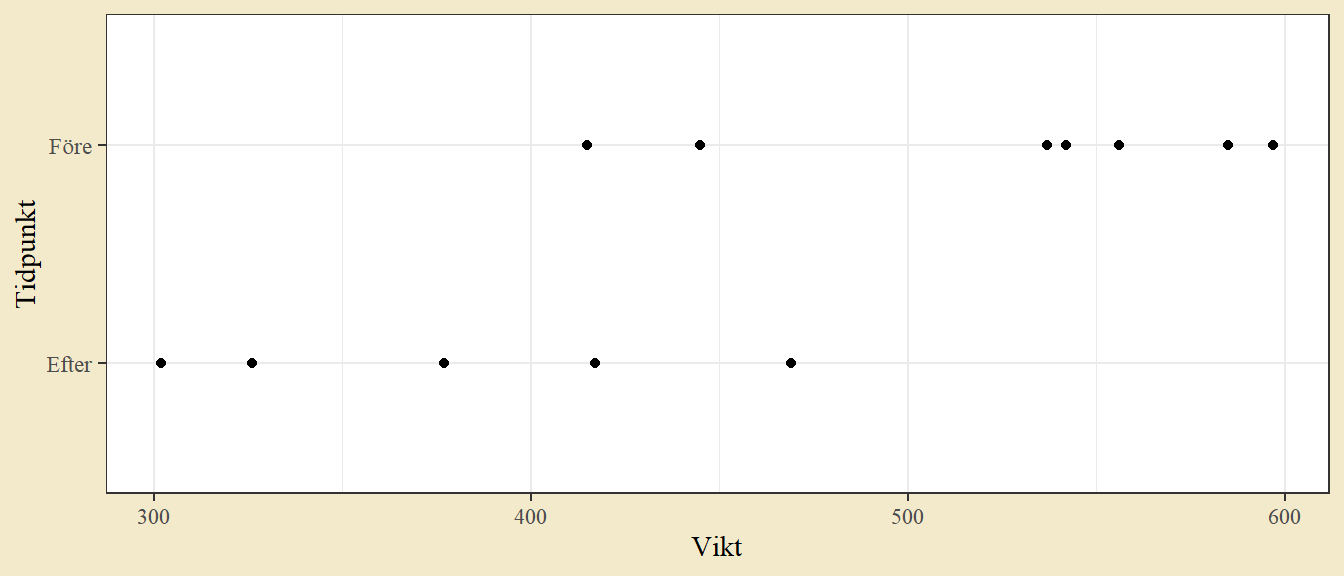
\includegraphics{R-anvisningar_files/figure-latex/unnamed-chunk-162-1} \end{center}

Grafen visar på högre vikter före vintern.

a. Ett konfidensintervall kan skapas genom att filtrera datan för observationerna före vintern och sedan skapa intervallet med \texttt{t.test}.

\begin{Shaded}
\begin{Highlighting}[]
\NormalTok{dat\_före }\OtherTok{\textless{}{-}}\NormalTok{ dat }\SpecialCharTok{\%\textgreater{}\%} \FunctionTok{filter}\NormalTok{(Tidpunkt }\SpecialCharTok{==} \StringTok{"Före"}\NormalTok{)}
\FunctionTok{t.test}\NormalTok{(dat\_före}\SpecialCharTok{$}\NormalTok{Vikt)}
\end{Highlighting}
\end{Shaded}

\begin{verbatim}
## 
##  One Sample t-test
## 
## data:  dat_före$Vikt
## t = 20.103, df = 6, p-value = 9.84e-07
## alternative hypothesis: true mean is not equal to 0
## 95 percent confidence interval:
##  461.3470 589.2244
## sample estimates:
## mean of x 
##  525.2857
\end{verbatim}

Utskriften ger intervallet \((461.35, 589.22)\), vilket ger tolkningen att populationsmedelvärdet för ekorrvikt före vintern ligger i det intervallet med 95 procents konfidens.

b. Datan är på lång form - ett t-test genomförs enklast med formelskrivningen \texttt{Vikt\ \textasciitilde{}\ Tidpunkt}. Testet kan genomföras med eller utan antagandet om lika varianser i grupperna.

\begin{Shaded}
\begin{Highlighting}[]
\FunctionTok{t.test}\NormalTok{(Vikt }\SpecialCharTok{\textasciitilde{}}\NormalTok{ Tidpunkt, dat)}
\end{Highlighting}
\end{Shaded}

\begin{verbatim}
## 
##  Welch Two Sample t-test
## 
## data:  Vikt by Tidpunkt
## t = -3.6807, df = 8.8977, p-value = 0.00517
## alternative hypothesis: true difference in means between group Efter and group Före is not equal to 0
## 95 percent confidence interval:
##  -237.64404  -56.52739
## sample estimates:
## mean in group Efter  mean in group Före 
##            378.2000            525.2857
\end{verbatim}

\begin{Shaded}
\begin{Highlighting}[]
\FunctionTok{t.test}\NormalTok{(Vikt }\SpecialCharTok{\textasciitilde{}}\NormalTok{ Tidpunkt, dat, }\AttributeTok{var.equal =}\NormalTok{ T)}
\end{Highlighting}
\end{Shaded}

\begin{verbatim}
## 
##  Two Sample t-test
## 
## data:  Vikt by Tidpunkt
## t = -3.6656, df = 10, p-value = 0.004348
## alternative hypothesis: true difference in means between group Efter and group Före is not equal to 0
## 95 percent confidence interval:
##  -236.49116  -57.68027
## sample estimates:
## mean in group Efter  mean in group Före 
##            378.2000            525.2857
\end{verbatim}

c. Om man mäter samma individ före och efter vintern och sedan analyserar viktförändringen över tid försvinner variansen \emph{mellan} individer.
\end{hypothesis}

\begin{exercise}[Burfågel]
I en undersökning av lungcancerpatienter finner man följande antal.

\begin{table}
\centering
\begin{tabular}[t]{lrr}
\toprule
  & Lungcancer & Ej lungcancer\\
\midrule
Burfågel & 98 & 101\\
Ej burfågel & 141 & 328\\
\bottomrule
\end{tabular}
\end{table}

Genomför ett test för att se om andelen burfågelägare än densamma i de två grupperna.
\end{exercise}

\begin{hypothesis}[Burfågel]
Frågan är om proportionen burfågelägare bland patienter är densamma som proportionen burfågelägare bland icke-drabbade. Man ska alltså ställa proportionen 98 av 239 mot 101 av 429.

\begin{Shaded}
\begin{Highlighting}[]
\FunctionTok{prop.test}\NormalTok{(}\FunctionTok{c}\NormalTok{(}\DecValTok{98}\NormalTok{, }\DecValTok{101}\NormalTok{), }\FunctionTok{c}\NormalTok{(}\DecValTok{98} \SpecialCharTok{+} \DecValTok{141}\NormalTok{, }\DecValTok{101} \SpecialCharTok{+} \DecValTok{328}\NormalTok{), }\AttributeTok{correct =}\NormalTok{ F)}
\end{Highlighting}
\end{Shaded}

\begin{verbatim}
## 
##  2-sample test for equality of proportions without continuity
##  correction
## 
## data:  c(98, 101) out of c(98 + 141, 101 + 328)
## X-squared = 22.374, df = 1, p-value = 2.244e-06
## alternative hypothesis: two.sided
## 95 percent confidence interval:
##  0.1004485 0.2487727
## sample estimates:
##    prop 1    prop 2 
## 0.4100418 0.2354312
\end{verbatim}

Det låga p-värdet tyder på att det finns skillnader mellan grupperna.
\end{hypothesis}

\begin{exercise}[Po-ta-toes]
I en undersökning på potatis används fyra behandlingar (a1b1, a1b2, a2b1 och a2b2). 125 potatisar från varje behandling sorteras in i fyra olika färggrupper (A, B, C och D). Frekvenstabellen ges av följande.

\begin{table}
\centering
\begin{tabular}[t]{lrrrr}
\toprule
Färg & a1b1 & a1b2 & a2b1 & a2b2\\
\midrule
A & 56 & 64 & 36 & 38\\
B & 45 & 36 & 44 & 48\\
C & 18 & 13 & 27 & 20\\
D & 6 & 12 & 18 & 19\\
\bottomrule
\end{tabular}
\end{table}

Genomför ett lämpligt test för att se om det finns färgskillnader mellan behandlingarna.
\end{exercise}

\begin{hypothesis}[Po-ta-toes]

Funktionen \texttt{matrix} kan användas för att skapa korstabellen. Tabellen kan sedan tas som ingångsvärde till \texttt{chisq.test}.

\begin{Shaded}
\begin{Highlighting}[]
\NormalTok{dat }\OtherTok{\textless{}{-}} \FunctionTok{matrix}\NormalTok{(}\FunctionTok{c}\NormalTok{(}\DecValTok{56}\NormalTok{,}\DecValTok{64}\NormalTok{,}\DecValTok{36}\NormalTok{,}\DecValTok{38}\NormalTok{,}
                \DecValTok{45}\NormalTok{,}\DecValTok{36}\NormalTok{,}\DecValTok{44}\NormalTok{,}\DecValTok{48}\NormalTok{,}
                \DecValTok{18}\NormalTok{,}\DecValTok{13}\NormalTok{,}\DecValTok{27}\NormalTok{,}\DecValTok{20}\NormalTok{,}
                \DecValTok{6}\NormalTok{,}\DecValTok{12}\NormalTok{,}\DecValTok{18}\NormalTok{,}\DecValTok{19}\NormalTok{),}
              \AttributeTok{nrow =} \DecValTok{4}\NormalTok{, }\AttributeTok{byrow =}\NormalTok{ T)}

\NormalTok{test }\OtherTok{\textless{}{-}} \FunctionTok{chisq.test}\NormalTok{(dat)}
\NormalTok{test}
\end{Highlighting}
\end{Shaded}

\begin{verbatim}
## 
##  Pearson's Chi-squared test
## 
## data:  dat
## X-squared = 26.518, df = 9, p-value = 0.00168
\end{verbatim}

I ett \(\chi^2\)-test är nollhypotesen att kolumner och rader är oberoende. Det låga p-värdet tyder på att nollhypotesen bör förkastas, vilket tyder på att det finns ett samband mellan behandling och färg.

Datan kan illustreras med ett stapeldiagram.

\begin{Shaded}
\begin{Highlighting}[]
\NormalTok{dat\_long }\OtherTok{\textless{}{-}}\NormalTok{ dat }\SpecialCharTok{\%\textgreater{}\%} 
  \FunctionTok{as\_tibble}\NormalTok{() }\SpecialCharTok{\%\textgreater{}\%} 
  \FunctionTok{mutate}\NormalTok{(Färg }\OtherTok{=} \FunctionTok{c}\NormalTok{(}\StringTok{"A"}\NormalTok{, }\StringTok{"B"}\NormalTok{, }\StringTok{"C"}\NormalTok{, }\StringTok{"D"}\NormalTok{)) }\SpecialCharTok{\%\textgreater{}\%} 
  \FunctionTok{pivot\_longer}\NormalTok{(}\SpecialCharTok{{-}}\NormalTok{Färg)}

\FunctionTok{ggplot}\NormalTok{(dat\_long, }\FunctionTok{aes}\NormalTok{(name, value, }\AttributeTok{fill =}\NormalTok{ Färg)) }\SpecialCharTok{+}
  \FunctionTok{geom\_bar}\NormalTok{(}\AttributeTok{stat =} \StringTok{"identity"}\NormalTok{, }\AttributeTok{col =} \StringTok{"black"}\NormalTok{, }\AttributeTok{width =} \FloatTok{0.6}\NormalTok{) }\SpecialCharTok{+}
  \FunctionTok{scale\_fill\_brewer}\NormalTok{(}\AttributeTok{palette =} \StringTok{"Reds"}\NormalTok{)}
\end{Highlighting}
\end{Shaded}

\begin{center}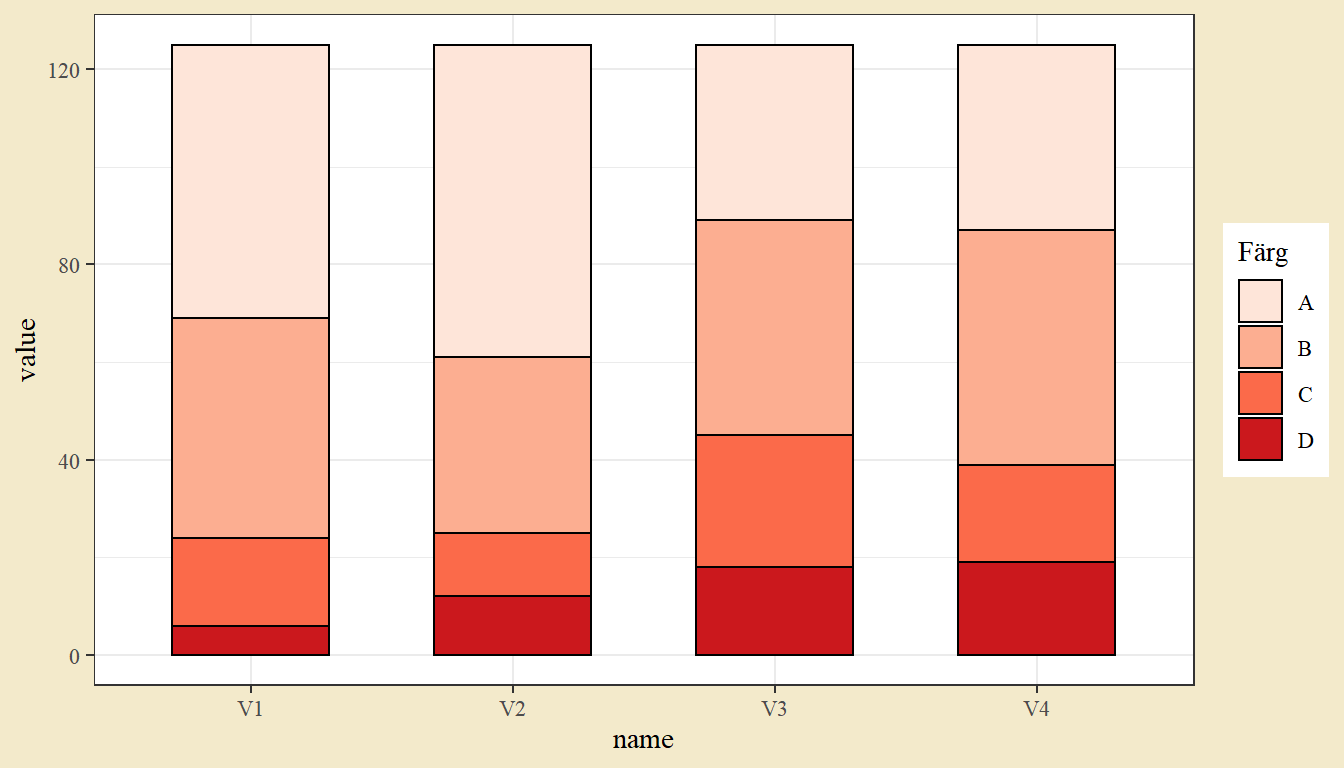
\includegraphics{R-anvisningar_files/figure-latex/unnamed-chunk-169-1} \end{center}

\end{hypothesis}

\begin{exercise}[Mer burfågel]
En tidigare uppgift gav följande data kring en eventuell koppling mellan fågelägande och lungcancer.

\begin{table}
\centering
\begin{tabular}[t]{lrr}
\toprule
  & Lungcancer & Ej lungcancer\\
\midrule
Burfågel & 98 & 101\\
Ej burfågel & 141 & 328\\
\bottomrule
\end{tabular}
\end{table}

Genomför ett \(\chi^2\)-test för att se om det finns något signifikant samband mellan variablerna.
\end{exercise}

\begin{hypothesis}[Mer burfågel]
För att genomföra \(\chi^2\)-testet kan man skriva in data som en 2-gånger-2-matris med funktionen \texttt{matrix}.

\begin{Shaded}
\begin{Highlighting}[]
\NormalTok{dat }\OtherTok{\textless{}{-}} \FunctionTok{matrix}\NormalTok{(}\FunctionTok{c}\NormalTok{(}\DecValTok{98}\NormalTok{, }\DecValTok{141}\NormalTok{, }\DecValTok{101}\NormalTok{, }\DecValTok{328}\NormalTok{), }\AttributeTok{nrow =} \DecValTok{2}\NormalTok{)}
\FunctionTok{chisq.test}\NormalTok{(dat, }\AttributeTok{correct =}\NormalTok{ F)}
\end{Highlighting}
\end{Shaded}

\begin{verbatim}
## 
##  Pearson's Chi-squared test
## 
## data:  dat
## X-squared = 22.374, df = 1, p-value = 2.244e-06
\end{verbatim}

Samma resultat som i den tidigare beräkningen på samma data.
\end{hypothesis}

\begin{exercise}[Allsvenskan. Genomsnittligt antal mål]
Bland kursdata finns datafiler med allsvenska matcher för damer (2000-2020) och herrar (1924-2019).
Det genomsnittliga antalet mål i respektive serie ges för åren 2000-2009 av följande tabell.

\begin{Shaded}
\begin{Highlighting}[]
\NormalTok{dat\_dam }\OtherTok{\textless{}{-}} \FunctionTok{read\_csv}\NormalTok{(}\StringTok{"Data/Allsvenskan, damer, 2000{-}2020.csv"}\NormalTok{)}
\NormalTok{dat\_herr }\OtherTok{\textless{}{-}} \FunctionTok{read\_csv}\NormalTok{(}\StringTok{"Data/Allsvenskan, herrar, 1924{-}2019.csv"}\NormalTok{)}

\NormalTok{dat\_dam\_medel }\OtherTok{\textless{}{-}}\NormalTok{ dat\_dam }\SpecialCharTok{\%\textgreater{}\%} 
  \FunctionTok{group\_by}\NormalTok{(sasong) }\SpecialCharTok{\%\textgreater{}\%} 
  \FunctionTok{summarise}\NormalTok{(Mål }\OtherTok{=} \FunctionTok{mean}\NormalTok{(hemmamal }\SpecialCharTok{+}\NormalTok{ bortamal)) }\SpecialCharTok{\%\textgreater{}\%} 
  \FunctionTok{filter}\NormalTok{(sasong }\SpecialCharTok{\%in\%} \DecValTok{2000}\SpecialCharTok{:}\DecValTok{2009}\NormalTok{)}

\NormalTok{dat\_herr\_medel }\OtherTok{\textless{}{-}}\NormalTok{ dat\_herr }\SpecialCharTok{\%\textgreater{}\%} 
  \FunctionTok{group\_by}\NormalTok{(sasong) }\SpecialCharTok{\%\textgreater{}\%} 
  \FunctionTok{summarise}\NormalTok{(Mål }\OtherTok{=} \FunctionTok{mean}\NormalTok{(hemmamal }\SpecialCharTok{+}\NormalTok{ bortamal)) }\SpecialCharTok{\%\textgreater{}\%} 
  \FunctionTok{filter}\NormalTok{(sasong }\SpecialCharTok{\%in\%} \DecValTok{2000}\SpecialCharTok{:}\DecValTok{2009}\NormalTok{) }\SpecialCharTok{\%\textgreater{}\%} 
  \FunctionTok{mutate}\NormalTok{(}\AttributeTok{sasong =} \FunctionTok{as.numeric}\NormalTok{(sasong))}

\NormalTok{dat\_total }\OtherTok{\textless{}{-}}\NormalTok{ dat\_dam\_medel }\SpecialCharTok{\%\textgreater{}\%}
  \FunctionTok{mutate}\NormalTok{(}\AttributeTok{Allsvenska =} \StringTok{"Dam"}\NormalTok{) }\SpecialCharTok{\%\textgreater{}\%} 
  \FunctionTok{bind\_rows}\NormalTok{(dat\_herr\_medel }\SpecialCharTok{\%\textgreater{}\%} \FunctionTok{mutate}\NormalTok{(}\AttributeTok{Allsvenska =} \StringTok{"Herr"}\NormalTok{)) }\SpecialCharTok{\%\textgreater{}\%} 
  \FunctionTok{rename}\NormalTok{(Säsong }\OtherTok{=}\NormalTok{ sasong)}

\NormalTok{dat\_total }\SpecialCharTok{\%\textgreater{}\%} 
  \FunctionTok{pivot\_wider}\NormalTok{(}\AttributeTok{values\_from =}\NormalTok{ Mål, }\AttributeTok{names\_from =}\NormalTok{ Allsvenska) }\SpecialCharTok{\%\textgreater{}\%} 
  \FunctionTok{kable}\NormalTok{(}\AttributeTok{digits =} \DecValTok{2}\NormalTok{)}
\end{Highlighting}
\end{Shaded}

\begin{table}
\centering
\begin{tabular}[t]{rrr}
\toprule
Säsong & Dam & Herr\\
\midrule
2000 & 3.68 & 2.87\\
2001 & 3.72 & 2.94\\
2002 & 3.65 & 2.81\\
2003 & 3.97 & 2.85\\
2004 & 3.65 & 2.43\\
\addlinespace
2005 & 3.54 & 2.68\\
2006 & 3.17 & 2.58\\
2007 & 3.37 & 2.56\\
2008 & 3.38 & 2.65\\
2009 & 3.33 & 2.43\\
\bottomrule
\end{tabular}
\end{table}

a. Jämför serierna med en lämplig graf.

b. Beräkna ett konfidensintervall för det genomsnittliga antalet mål i allsvenskan för damer.

c. Genomför ett lämpligt test för att se om serierna har samma populationsmedelvärde för antal mål. Diskutera om datan bör ses som parad (två observationer per år).
\end{exercise}

\begin{hypothesis}[Allsvenskan. Genomsnittligt antal mål]
a. Datan kan illustreras med ett linjediagram med två separata linjer.

\begin{Shaded}
\begin{Highlighting}[]
\CommentTok{\# Fortsättning från inläsningen ovan}
\FunctionTok{ggplot}\NormalTok{(dat\_total, }\FunctionTok{aes}\NormalTok{(Säsong, Mål, }\AttributeTok{col =}\NormalTok{ Allsvenska)) }\SpecialCharTok{+}
  \FunctionTok{geom\_line}\NormalTok{(}\AttributeTok{size =} \DecValTok{2}\NormalTok{)}
\end{Highlighting}
\end{Shaded}

\begin{center}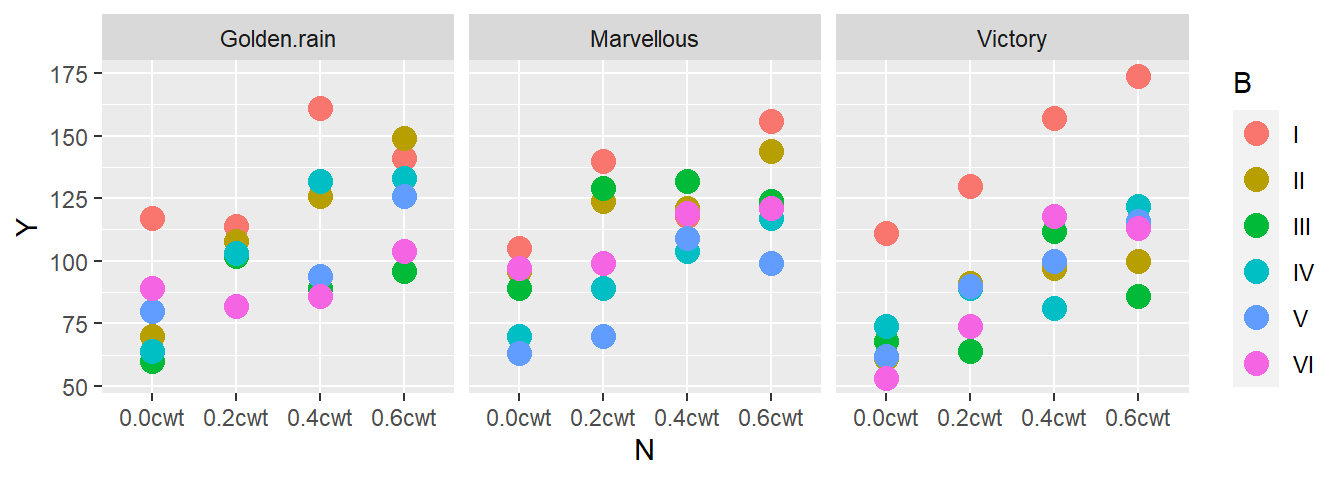
\includegraphics{R-anvisningar_files/figure-latex/unnamed-chunk-173-1} \end{center}

Allsvenskan för damer har ett högre genomsnittligt antal mål än allsvenskan för herrar.

b. Konfidensintervall kan beräknas med \texttt{t.test} efter att observationer för damer filtrerats ut.

\begin{Shaded}
\begin{Highlighting}[]
\NormalTok{dat }\OtherTok{\textless{}{-}}\NormalTok{ dat\_total }\SpecialCharTok{\%\textgreater{}\%} \FunctionTok{filter}\NormalTok{(Allsvenska }\SpecialCharTok{==} \StringTok{"Dam"}\NormalTok{)}
\FunctionTok{t.test}\NormalTok{(dat}\SpecialCharTok{$}\NormalTok{Mål)}
\end{Highlighting}
\end{Shaded}

\begin{verbatim}
## 
##  One Sample t-test
## 
## data:  dat$Mål
## t = 47.784, df = 9, p-value = 3.858e-12
## alternative hypothesis: true mean is not equal to 0
## 95 percent confidence interval:
##  3.378329 3.714095
## sample estimates:
## mean of x 
##  3.546212
\end{verbatim}

Konfidensintervallet ges av \((3.37, 3.71)\). Det sanna populationsmedelvärdet ligger med 95-procents konfidens i det intervallet.

c. Ett lämpligt test kan genomföras med \texttt{t.test}. Nollhypotesen är att serierna har samma populationsmedelvärde och att den skillnad man kan se därmed enbart är slumpmässig variation.

\begin{Shaded}
\begin{Highlighting}[]
\FunctionTok{t.test}\NormalTok{(Mål }\SpecialCharTok{\textasciitilde{}}\NormalTok{ Allsvenska, dat\_total)}
\end{Highlighting}
\end{Shaded}

\begin{verbatim}
## 
##  Welch Two Sample t-test
## 
## data:  Mål by Allsvenska
## t = 9.24, df = 16.897, p-value = 5.129e-08
## alternative hypothesis: true difference in means between group Dam and group Herr is not equal to 0
## 95 percent confidence interval:
##  0.6677709 1.0631973
## sample estimates:
##  mean in group Dam mean in group Herr 
##           3.546212           2.680728
\end{verbatim}

Det låga p-värdet ger att nollhypotesen bör förkastas - man kan dra slutsatsen att allsvenskan för damer har högre genomsnittligt antal mål än allsvenskan för herrar.

I det här fallet kan man diskutera om det inte är mer lämpligt att använda ett t-test för parade observation, eftersom det är två observationer per år. Ett argument mot det är att det inte finns någon egentlig anledning att tro att det skulle finnas något samband mellan antal mål för damer respektive för herrar ett visst år.
\end{hypothesis}

\begin{exercise}[Nature's mosquito]
En viktig del i arbetet mot spridning av malaria är att förstå myggors reaktion på dofter. Ett vanligt sätt att undersöka detta är att följa flyktmönster i en sluten vindtunnel. I ett försök har man en vindtunnel med måtten 60 x 30 x 100 cm (bredd, höjd, djup). I den ena änden finns två doftkällor placerade i jämn höjd, med 30 centimeters mellanrum. I den andra änden släpper man en mygga i taget och genom videoinspelning kan man beräkna dess position varje tiondels sekund. Försöket omfattar 60 individer av två arter. Datan finns tillgänglig bland kursdatan i filen \emph{Mosquitos.csv}.

a. Illustrera en eller flera myggors flykt med ett passande diagram. En möjlighet är att ha z-koordinaten på den horisontella axeln och x-koordinaten på den vertikala axeln och göra en spårlinje med \texttt{geom\_path}. Den linjen motsvarar då flykten sedd från ovan. Eftersom flykten anges med x-, y- och z-koordinater kan man även illustrera det som en tre-dimensionell graf, till exempel med \texttt{rgl}-paketet.

b. Det är möjligt att ta fram myggornas landningspunkt på bortre änden genom att filtera på värden där \texttt{Proportional\_time} är 1. Man får då följande värden på x-koordinaten.

\begin{table}
\centering
\begin{tabular}[t]{rr}
\toprule
Aedes africanus & Aedes aegypti\\
\midrule
-9.94 & 8.54\\
-10.75 & 1.18\\
-4.97 & -1.55\\
-3.50 & -1.65\\
-3.63 & 7.64\\
\addlinespace
-11.39 & 4.99\\
-15.98 & -3.77\\
2.01 & 4.53\\
-13.19 & 3.18\\
-4.51 & 9.63\\
\addlinespace
-6.17 & 5.83\\
-11.56 & -0.26\\
-5.38 & 3.71\\
-3.88 & 3.07\\
-1.83 & 5.15\\
\addlinespace
-4.04 & 0.02\\
-5.80 & -0.45\\
2.12 & -5.83\\
-13.67 & 7.14\\
-14.61 & 12.28\\
\addlinespace
-3.46 & -3.50\\
-8.02 & 5.83\\
0.20 & 1.43\\
-14.54 & -8.64\\
-17.62 & 5.14\\
\addlinespace
-10.41 & -0.11\\
1.03 & 13.40\\
-6.06 & 14.80\\
-3.41 & -6.91\\
-0.48 & 8.38\\
\bottomrule
\end{tabular}
\end{table}

Konstruera ett lådagram över x-koordinaterna för de 60 individerna vid landningstillfället. Dela grafen så att arterna visas i skilda lådagram. Finns det tecken på skillnader i landningspunkt?

c. Genomför ett lämpligt t-test för att se om det finns skillnader mellan arterna, med avseende på x-koordinat vid landningstillfället.

d. Konstruera ett konfidensintervall för medelvärdet av x-koordinaten vid landning för \emph{Aedes aegypti}. Använd intervallet för att se om medelvärdet är statistiskt signifikant skilt från 0.

e. Om man bara sorterar individer efter om de landar på den högra eller vänstra halvan av den borde änden kan man ställa upp följande korstabell.

\begin{table}
\centering
\begin{tabular}[t]{lrr}
\toprule
Species & Left & Right\\
\midrule
Aedes aegypti & 10 & 20\\
Aedes africanus & 26 & 4\\
\bottomrule
\end{tabular}
\end{table}

Genomför ett lämpligt z-test eller \(\chi^2\)-test för att se om det finns en statistiskt säkerställd skillnad i landningsposition mellan arterna.

Frågan är baserad på Hinze et al (2021) \emph{Mosquito Host Seeking in 3D Using a Versatile Climate-Controlled Wind Tunnel System}.
\end{exercise}

\begin{hypothesis}[Nature's mosquito]
Datan importas med \texttt{read\_csv}.

\begin{Shaded}
\begin{Highlighting}[]
\NormalTok{dat }\OtherTok{\textless{}{-}} \FunctionTok{read\_csv}\NormalTok{(}\StringTok{"Data/Mosquitos.csv"}\NormalTok{)}
\end{Highlighting}
\end{Shaded}

a. En passande graf kan konstrueras med \texttt{ggplot2} och \texttt{geom\_path}. Med två grafer kan man illustrera flykten från sidan och från ovan. Färger kan separera arterna. Den specifika individen måste sättas med \texttt{group\ =\ id} för att den enskilda flykten ska bli en egen linje.

Ett exempel på en enskild individ.

\begin{Shaded}
\begin{Highlighting}[]
\NormalTok{dat\_ind1 }\OtherTok{\textless{}{-}}\NormalTok{ dat }\SpecialCharTok{\%\textgreater{}\%} \FunctionTok{filter}\NormalTok{(id }\SpecialCharTok{==} \DecValTok{1}\NormalTok{)}

\NormalTok{g1 }\OtherTok{\textless{}{-}} \FunctionTok{ggplot}\NormalTok{(dat\_ind1, }\FunctionTok{aes}\NormalTok{(z, y, }\AttributeTok{group =}\NormalTok{ id, }\AttributeTok{col =}\NormalTok{ Species)) }\SpecialCharTok{+} 
  \FunctionTok{geom\_path}\NormalTok{() }\SpecialCharTok{+}
  \FunctionTok{labs}\NormalTok{(}\AttributeTok{title =} \StringTok{"Från sidan"}\NormalTok{)}

\NormalTok{g2 }\OtherTok{\textless{}{-}} \FunctionTok{ggplot}\NormalTok{(dat\_ind1, }\FunctionTok{aes}\NormalTok{(z, x, }\AttributeTok{group =}\NormalTok{ id, }\AttributeTok{col =}\NormalTok{ Species)) }\SpecialCharTok{+} 
  \FunctionTok{geom\_path}\NormalTok{() }\SpecialCharTok{+}
  \FunctionTok{labs}\NormalTok{(}\AttributeTok{title =} \StringTok{"Från ovan"}\NormalTok{)}

\FunctionTok{library}\NormalTok{(patchwork)}
\NormalTok{g1 }\SpecialCharTok{/}\NormalTok{ g2}
\end{Highlighting}
\end{Shaded}

\begin{center}\includegraphics{R-anvisningar_files/figure-latex/unnamed-chunk-179-1} \end{center}

Ett exempel med samtliga individer i en (rörig) illustration.

\begin{Shaded}
\begin{Highlighting}[]
\NormalTok{g1 }\OtherTok{\textless{}{-}} \FunctionTok{ggplot}\NormalTok{(dat, }\FunctionTok{aes}\NormalTok{(z, y, }\AttributeTok{group =}\NormalTok{ id, }\AttributeTok{col =}\NormalTok{ Species)) }\SpecialCharTok{+} 
  \FunctionTok{geom\_path}\NormalTok{(}\AttributeTok{alpha =} \FloatTok{0.5}\NormalTok{) }\SpecialCharTok{+}
  \FunctionTok{labs}\NormalTok{(}\AttributeTok{title =} \StringTok{"Från sidan"}\NormalTok{)}

\NormalTok{g2 }\OtherTok{\textless{}{-}} \FunctionTok{ggplot}\NormalTok{(dat, }\FunctionTok{aes}\NormalTok{(z, x, }\AttributeTok{group =}\NormalTok{ id, }\AttributeTok{col =}\NormalTok{ Species)) }\SpecialCharTok{+} 
  \FunctionTok{geom\_path}\NormalTok{(}\AttributeTok{alpha =} \FloatTok{0.5}\NormalTok{) }\SpecialCharTok{+}
  \FunctionTok{labs}\NormalTok{(}\AttributeTok{title =} \StringTok{"Från ovan"}\NormalTok{)}

\FunctionTok{library}\NormalTok{(patchwork)}
\NormalTok{g1 }\SpecialCharTok{/}\NormalTok{ g2}
\end{Highlighting}
\end{Shaded}

\begin{center}\includegraphics{R-anvisningar_files/figure-latex/unnamed-chunk-180-1} \end{center}

R har paket med funktioner för tre-dimensionella grafer. Ett exempel är genom paketet \texttt{rgl} och funktionerna \texttt{plot3d} och \texttt{lines3d}.

\begin{Shaded}
\begin{Highlighting}[]
\CommentTok{\# install.packages(rgl)}
\FunctionTok{library}\NormalTok{(rgl)}
\CommentTok{\# En enskild mygga plottad med plot3d}
\CommentTok{\# Det första argumentet är de tre koordinatvariablerna efter filter på första individen}
\FunctionTok{plot3d}\NormalTok{(dat }\SpecialCharTok{\%\textgreater{}\%} \FunctionTok{filter}\NormalTok{(id }\SpecialCharTok{==} \DecValTok{1}\NormalTok{) }\SpecialCharTok{\%\textgreater{}\%} \FunctionTok{select}\NormalTok{(z, x, y), }\AttributeTok{type =} \StringTok{"l"}\NormalTok{, }\AttributeTok{asp =}\NormalTok{ F, }\AttributeTok{col =} \StringTok{"blue"}\NormalTok{, }\AttributeTok{alpha =} \FloatTok{0.15}\NormalTok{)}

\CommentTok{\# Övriga flykter tillagda med lines3d i en for{-}loop}
\CommentTok{\# Loopen går inom samtliga individer och lägger till linjen till 3d{-}grafen}
\ControlFlowTok{for}\NormalTok{(i }\ControlFlowTok{in} \DecValTok{1}\SpecialCharTok{:}\DecValTok{60}\NormalTok{)\{}
  \FunctionTok{lines3d}\NormalTok{(dat }\SpecialCharTok{\%\textgreater{}\%} \FunctionTok{filter}\NormalTok{(id }\SpecialCharTok{==}\NormalTok{ i) }\SpecialCharTok{\%\textgreater{}\%} \FunctionTok{select}\NormalTok{(z, x, y), }
          \AttributeTok{col =} \FunctionTok{ifelse}\NormalTok{(dat }\SpecialCharTok{\%\textgreater{}\%} \FunctionTok{filter}\NormalTok{(id }\SpecialCharTok{==}\NormalTok{ i) }\SpecialCharTok{\%\textgreater{}\%} \FunctionTok{pull}\NormalTok{(Species) }\SpecialCharTok{==} \StringTok{"Aedes africanus"}\NormalTok{, }\StringTok{"blue"}\NormalTok{, }\StringTok{"red"}\NormalTok{),}
          \AttributeTok{alpha =} \FloatTok{0.15}\NormalTok{)}
\NormalTok{\}}

\CommentTok{\# Skapa punkter för landningsplatsen}
\FunctionTok{points3d}\NormalTok{(dat }\SpecialCharTok{\%\textgreater{}\%} \FunctionTok{filter}\NormalTok{(Proportional\_time }\SpecialCharTok{==} \DecValTok{1}\NormalTok{) }\SpecialCharTok{\%\textgreater{}\%} \FunctionTok{select}\NormalTok{(z, x, y), }\AttributeTok{size =} \DecValTok{6}\NormalTok{, }
         \AttributeTok{col =} \FunctionTok{ifelse}\NormalTok{(dat }\SpecialCharTok{\%\textgreater{}\%} \FunctionTok{filter}\NormalTok{(Proportional\_time }\SpecialCharTok{==} \DecValTok{1}\NormalTok{) }\SpecialCharTok{\%\textgreater{}\%} \FunctionTok{pull}\NormalTok{(Species) }\SpecialCharTok{==} \StringTok{"Aedes africanus"}\NormalTok{, }\StringTok{"blue"}\NormalTok{, }\StringTok{"red"}\NormalTok{))}
\end{Highlighting}
\end{Shaded}

b. För att titta på landningsplatser filtreras på de observationer där den proportionella observationstiden är 1 (den sista observationen). Därefter kan en lämplig graf skapas med \texttt{geom\_boxplot} med art på x-axeln och x-koordinaten på grafens y-axel.

\begin{Shaded}
\begin{Highlighting}[]
\NormalTok{dat\_endtime }\OtherTok{\textless{}{-}}\NormalTok{ dat }\SpecialCharTok{\%\textgreater{}\%} \FunctionTok{filter}\NormalTok{(Proportional\_time }\SpecialCharTok{==} \DecValTok{1}\NormalTok{)}

\FunctionTok{ggplot}\NormalTok{(dat\_endtime, }\FunctionTok{aes}\NormalTok{(Species, x)) }\SpecialCharTok{+} \FunctionTok{geom\_boxplot}\NormalTok{()}
\end{Highlighting}
\end{Shaded}

\begin{center}\includegraphics{R-anvisningar_files/figure-latex/unnamed-chunk-182-1} \end{center}

\emph{Aedes aegypti} uppvisar högre x-koordinater, vilket tyder på att den arten varit mer lockad av doftämnet till höger.

c. Ett t-test för oberoende stickprov kan genomföras genom att ta x-koordinaten som utfallsvariabel och arterna som de två grupperna. Testet kan genomföras med eller utan antaganden om lika varianser inom grupperna. Nollhypotesen är arterna har samma populationsmedelvärde i x-koordinaten vid landningstillfället.

\begin{Shaded}
\begin{Highlighting}[]
\FunctionTok{t.test}\NormalTok{(x }\SpecialCharTok{\textasciitilde{}}\NormalTok{ Species, dat\_endtime)}
\end{Highlighting}
\end{Shaded}

\begin{verbatim}
## 
##  Welch Two Sample t-test
## 
## data:  x by Species
## t = 6.7001, df = 57.845, p-value = 9.436e-09
## alternative hypothesis: true difference in means between group Aedes aegypti and group Aedes africanus is not equal to 0
## 95 percent confidence interval:
##   6.93371 12.84229
## sample estimates:
##   mean in group Aedes aegypti mean in group Aedes africanus 
##                      3.106667                     -6.781333
\end{verbatim}

\begin{Shaded}
\begin{Highlighting}[]
\FunctionTok{t.test}\NormalTok{(x }\SpecialCharTok{\textasciitilde{}}\NormalTok{ Species, dat\_endtime, }\AttributeTok{var.equal =}\NormalTok{ T)}
\end{Highlighting}
\end{Shaded}

\begin{verbatim}
## 
##  Two Sample t-test
## 
## data:  x by Species
## t = 6.7001, df = 58, p-value = 9.331e-09
## alternative hypothesis: true difference in means between group Aedes aegypti and group Aedes africanus is not equal to 0
## 95 percent confidence interval:
##   6.933879 12.842121
## sample estimates:
##   mean in group Aedes aegypti mean in group Aedes africanus 
##                      3.106667                     -6.781333
\end{verbatim}

Bägge testet ger stark signifikans. Man drar slutsatsen att det finns en skillnad mellan arterna.

d. Ett konfidensintervall kan tas fram med \texttt{t.test} efter filtrering på art så att enbart \emph{aegypti} förekommer i datan.

\begin{Shaded}
\begin{Highlighting}[]
\NormalTok{dat\_endtime\_aegypti }\OtherTok{\textless{}{-}}\NormalTok{ dat\_endtime }\SpecialCharTok{\%\textgreater{}\%} \FunctionTok{filter}\NormalTok{(Species }\SpecialCharTok{==} \StringTok{"Aedes aegypti"}\NormalTok{)}
\FunctionTok{t.test}\NormalTok{(dat\_endtime\_aegypti}\SpecialCharTok{$}\NormalTok{x)}
\end{Highlighting}
\end{Shaded}

\begin{verbatim}
## 
##  One Sample t-test
## 
## data:  dat_endtime_aegypti$x
## t = 2.9029, df = 29, p-value = 0.006996
## alternative hypothesis: true mean is not equal to 0
## 95 percent confidence interval:
##  0.9178614 5.2954719
## sample estimates:
## mean of x 
##  3.106667
\end{verbatim}

Intervallet ges av \((0.92, 5.30)\). Eftersom 0 inte ingår i det 95-procentiga konfidensintervallet är det statistiskt signifikant (på 5-procentsnivån) att populationsmedelvärdet skiljer sig från 0.

e. Antalet kan antingen skrivas in från siffrorna i uppgiften eller beräknas från data genom att koda om x-koordinaten till höger respektive vänster beroende på om x är större eller mindre än 0. Därefter kan ett test genomföras med \texttt{chisq.test}. Nollhypotesen är att populationsproportionen högergående (eller vänstergående) är lika stor för de två arterna.

\begin{Shaded}
\begin{Highlighting}[]
\NormalTok{dat\_prop }\OtherTok{\textless{}{-}}\NormalTok{ dat\_endtime }\SpecialCharTok{\%\textgreater{}\%} 
  \FunctionTok{count}\NormalTok{(Species, }\AttributeTok{Direction =} \FunctionTok{ifelse}\NormalTok{(x }\SpecialCharTok{\textless{}} \DecValTok{0}\NormalTok{, }\StringTok{"Left"}\NormalTok{, }\StringTok{"Right"}\NormalTok{)) }\SpecialCharTok{\%\textgreater{}\%} 
  \FunctionTok{pivot\_wider}\NormalTok{(}\AttributeTok{names\_from =}\NormalTok{ Direction, }\AttributeTok{values\_from =}\NormalTok{ n)}

\FunctionTok{chisq.test}\NormalTok{(dat\_prop }\SpecialCharTok{\%\textgreater{}\%} \FunctionTok{select}\NormalTok{(Left, Right))}
\end{Highlighting}
\end{Shaded}

\begin{verbatim}
## 
##  Pearson's Chi-squared test with Yates' continuity correction
## 
## data:  dat_prop %>% select(Left, Right)
## X-squared = 15.625, df = 1, p-value = 7.723e-05
\end{verbatim}

Testet pekar på en skillnad i proportionen höger- respektive vänstergående mellan arterna.
\end{hypothesis}

\begin{exercise}[Röda rummet, Gösta Berlings saga, och okänd]
Bland kursdatan finns text till Selma Lagerlöfs \emph{Gösta Berlings saga} och August Strindbergs \emph{Röda rummet}, i kolumnform. Det finns också en text med okänd författare (filen \emph{Den tredje boken}). En ytlig textanalys kan baseras på frekvensen för olika ord. Närliggande tabell ger antalet förekomster för texternas fem vanligaste ord i första kapitlet av varje text.

\begin{Shaded}
\begin{Highlighting}[]
\NormalTok{dat\_rr }\OtherTok{\textless{}{-}} \FunctionTok{read\_csv}\NormalTok{(}\StringTok{"Data/Röda rummet.csv"}\NormalTok{) }\SpecialCharTok{\%\textgreater{}\%} 
  \FunctionTok{mutate}\NormalTok{(}\AttributeTok{Bok =} \StringTok{"Röda rummet"}\NormalTok{)}
\NormalTok{dat\_gbs }\OtherTok{\textless{}{-}} \FunctionTok{read\_csv}\NormalTok{(}\StringTok{"Data/Gösta Berlings saga.csv"}\NormalTok{) }\SpecialCharTok{\%\textgreater{}\%} 
  \FunctionTok{mutate}\NormalTok{(}\AttributeTok{Bok =} \StringTok{"Gösta Berlings saga"}\NormalTok{)}
\NormalTok{dat\_tredje }\OtherTok{\textless{}{-}} \FunctionTok{read\_csv}\NormalTok{(}\StringTok{"Data/Den tredje boken.csv"}\NormalTok{) }\SpecialCharTok{\%\textgreater{}\%} 
  \FunctionTok{mutate}\NormalTok{(}\AttributeTok{Bok =} \StringTok{"Okänd"}\NormalTok{)}

\NormalTok{dat\_full }\OtherTok{\textless{}{-}} \FunctionTok{bind\_rows}\NormalTok{(dat\_rr, dat\_gbs, dat\_tredje)}
\NormalTok{vanligaste\_ord }\OtherTok{\textless{}{-}}\NormalTok{ dat\_full }\SpecialCharTok{\%\textgreater{}\%} 
  \FunctionTok{count}\NormalTok{(Ord, }\AttributeTok{sort =}\NormalTok{ T) }\SpecialCharTok{\%\textgreater{}\%}
  \FunctionTok{slice}\NormalTok{(}\DecValTok{1}\SpecialCharTok{:}\DecValTok{5}\NormalTok{) }\SpecialCharTok{\%\textgreater{}\%} 
  \FunctionTok{pull}\NormalTok{(Ord)}

\NormalTok{dat\_ord }\OtherTok{\textless{}{-}}\NormalTok{ dat\_full }\SpecialCharTok{\%\textgreater{}\%} 
  \FunctionTok{filter}\NormalTok{(Ord }\SpecialCharTok{\%in\%}\NormalTok{ vanligaste\_ord, Kapitel }\SpecialCharTok{==} \DecValTok{1}\NormalTok{) }\SpecialCharTok{\%\textgreater{}\%} 
  \FunctionTok{count}\NormalTok{(Bok, Ord) }

\NormalTok{dat\_ord\_wide }\OtherTok{\textless{}{-}}\NormalTok{ dat\_ord }\SpecialCharTok{\%\textgreater{}\%} 
  \FunctionTok{pivot\_wider}\NormalTok{(}\AttributeTok{names\_from =}\NormalTok{ Bok, }\AttributeTok{values\_from =}\NormalTok{ n) }\SpecialCharTok{\%\textgreater{}\%} 
  \FunctionTok{arrange}\NormalTok{(}\FunctionTok{desc}\NormalTok{(}\StringTok{\textasciigrave{}}\AttributeTok{Gösta Berlings saga}\StringTok{\textasciigrave{}} \SpecialCharTok{+}\NormalTok{ Okänd }\SpecialCharTok{+} \StringTok{\textasciigrave{}}\AttributeTok{Röda rummet}\StringTok{\textasciigrave{}}\NormalTok{))}
\FunctionTok{kable}\NormalTok{(dat\_ord\_wide)}
\end{Highlighting}
\end{Shaded}

\begin{table}
\centering
\begin{tabular}[t]{lrrr}
\toprule
Ord & Gösta Berlings saga & Okänd & Röda rummet\\
\midrule
och & 109 & 143 & 166\\
han & 116 & 115 & 52\\
att & 67 & 130 & 74\\
det & 46 & 91 & 63\\
i & 52 & 58 & 83\\
\bottomrule
\end{tabular}
\end{table}

a~Illustrera frekvenserna med en lämplig graf.

b. Genomför två \(\chi^2\)-test för att se vilken av Gösta Berlings saga och Röda rummet den okända texten är mest lik (sett till de fem vanligaste orden).
\end{exercise}

\begin{hypothesis}[Röda rummet, Gösta Berlings saga, och okänd]
a. En möjlig illustration är ett stapeldiagram för proportion av varje ord inom respektive text.

\begin{Shaded}
\begin{Highlighting}[]
\NormalTok{dat\_ord }\SpecialCharTok{\%\textgreater{}\%}
  \FunctionTok{ggplot}\NormalTok{(}\FunctionTok{aes}\NormalTok{(Bok, n, }\AttributeTok{fill =}\NormalTok{ Ord)) }\SpecialCharTok{+}
  \FunctionTok{geom\_bar}\NormalTok{(}\AttributeTok{stat =} \StringTok{"identity"}\NormalTok{, }\AttributeTok{position =} \FunctionTok{position\_fill}\NormalTok{(), }\AttributeTok{col =} \StringTok{"black"}\NormalTok{)}
\end{Highlighting}
\end{Shaded}

\begin{center}\includegraphics{R-anvisningar_files/figure-latex/unnamed-chunk-187-1} \end{center}

Röda rummet har större andel förekomster av \emph{och} och \emph{i}.

b. Två \(\chi^2\)-test kan användas för att ställa de kända verken mot det okända verket. Detta kan göras genom att välja kolumner från \texttt{dat\_ord\_wide} med hakparenteser.

\begin{Shaded}
\begin{Highlighting}[]
\CommentTok{\# Gösta Berlings saga (kolumn 2) mot okänd text (kolumn 3)}
\FunctionTok{chisq.test}\NormalTok{(dat\_ord\_wide[, }\DecValTok{2}\SpecialCharTok{:}\DecValTok{3}\NormalTok{])}
\end{Highlighting}
\end{Shaded}

\begin{verbatim}
## 
##  Pearson's Chi-squared test
## 
## data:  dat_ord_wide[, 2:3]
## X-squared = 16.963, df = 4, p-value = 0.001965
\end{verbatim}

\begin{Shaded}
\begin{Highlighting}[]
\CommentTok{\# Röda rummet (kolumn 4) mot okänd text (kolumn 3)}
\FunctionTok{chisq.test}\NormalTok{(dat\_ord\_wide[, }\DecValTok{3}\SpecialCharTok{:}\DecValTok{4}\NormalTok{])}
\end{Highlighting}
\end{Shaded}

\begin{verbatim}
## 
##  Pearson's Chi-squared test
## 
## data:  dat_ord_wide[, 3:4]
## X-squared = 40.742, df = 4, p-value = 3.039e-08
\end{verbatim}

Bägge testen förkastar nollhypotesen (som är att det inte finns några skillnader mellan verken i ordens relativa frekvenser), men det högre p-värdet i testet mot Gösta Berlings saga tyder på att det finns ett starkare samband mellan de texterna än mellan Röda rummet och den okända texten.
\end{hypothesis}

\hypertarget{variansanalys}{%
\chapter{Variansanalys}\label{variansanalys}}

Variansanalys (eller \emph{anova-modellen}) är en statistisk modell där medelvärdet varierar beroende på en behandling och ett normalfördelat slumpfel. Från en anova-modell kan man beräkna ett F-test, som testar om det finns någon övergripande gruppskillnad, och post-hoc-test, som jämför specifika grupper med varandra.

Den specifika modellen beror på försöksupplägget. Här ges exempel på variansanalys med en faktor, en faktor med block, och två faktorer.

\hypertarget{variansanalys.-en-faktor}{%
\section{Variansanalys. En faktor}\label{variansanalys.-en-faktor}}

Vid variansanalys med en faktor har man ett upplägg där varje observation av en kontinuerlig utfallsvariabel är kopplad till en specifik grupp. Som exempel används en datamängd från ett odlingsförsök på havre. Datan finns tillgänglig i paketet \texttt{MASS} som \texttt{oats}. Försöket är ett två-faktoriellt försök med block. Faktorerna ges av havresort och kvävetillsättning; utfallsvariabeln är skördvikt. Som första exempel ignoreras sortvariabeln genom att beräkna medelvärde per block och kvävenivå.

\begin{Shaded}
\begin{Highlighting}[]
\NormalTok{dat }\OtherTok{\textless{}{-}}\NormalTok{ MASS}\SpecialCharTok{::}\NormalTok{oats}
\NormalTok{dat }\OtherTok{\textless{}{-}}\NormalTok{ dat }\SpecialCharTok{\%\textgreater{}\%} 
  \FunctionTok{group\_by}\NormalTok{(B, N) }\SpecialCharTok{\%\textgreater{}\%} 
  \FunctionTok{summarise}\NormalTok{(}\AttributeTok{Y =} \FunctionTok{mean}\NormalTok{(Y)) }\SpecialCharTok{\%\textgreater{}\%} 
  \FunctionTok{ungroup}\NormalTok{() }\SpecialCharTok{\%\textgreater{}\%} 
  \FunctionTok{as\_tibble}\NormalTok{()}

\FunctionTok{kable}\NormalTok{(dat }\SpecialCharTok{\%\textgreater{}\%} \FunctionTok{pivot\_wider}\NormalTok{(}\AttributeTok{names\_from =}\NormalTok{ N, }\AttributeTok{values\_from =}\NormalTok{ Y), }
      \AttributeTok{digits =} \DecValTok{1}\NormalTok{)}
\end{Highlighting}
\end{Shaded}

\begin{table}
\centering
\begin{tabular}[t]{lrrrr}
\toprule
B & 0.0cwt & 0.2cwt & 0.4cwt & 0.6cwt\\
\midrule
I & 111.0 & 128.0 & 145.3 & 157.0\\
II & 75.7 & 107.7 & 114.7 & 131.0\\
III & 72.3 & 98.3 & 111.0 & 102.0\\
IV & 69.3 & 93.7 & 105.7 & 124.0\\
V & 68.3 & 80.7 & 101.0 & 113.7\\
\addlinespace
VI & 79.7 & 85.0 & 107.7 & 112.7\\
\bottomrule
\end{tabular}
\end{table}

Datan har 18 observationer av skördvikt och varje observation tillhör någon specifik kvävenivå. Datan kan illustreras med ett spridningsdiagram.

\begin{Shaded}
\begin{Highlighting}[]
\FunctionTok{ggplot}\NormalTok{(dat, }\FunctionTok{aes}\NormalTok{(N, Y)) }\SpecialCharTok{+}
  \FunctionTok{geom\_point}\NormalTok{()}
\end{Highlighting}
\end{Shaded}

\begin{center}\includegraphics{R-anvisningar_files/figure-latex/unnamed-chunk-190-1} \end{center}

Det finns en tydlig kväveeffekt.

En anova-modell kan i R skattas med funktionen \texttt{lm} (för \emph{linjär modell}). Från modellobjektet kan man sedan plocka fram en anova-tabell (som bland annat anger utfallet av F-testet) och genomföra parvisa jämförelser genom \texttt{emmeans}.

\begin{Shaded}
\begin{Highlighting}[]
\NormalTok{mod }\OtherTok{\textless{}{-}} \FunctionTok{lm}\NormalTok{(Y }\SpecialCharTok{\textasciitilde{}}\NormalTok{ N, }\AttributeTok{data =}\NormalTok{ dat)}
\end{Highlighting}
\end{Shaded}

Modellen anges som en formel \texttt{Y\ \textasciitilde{}\ N}, vilket kan utläsas \emph{Y beroende på faktorn N}. Detta följs av ett argument för det objekt som innehåller datan i kolumner (här \texttt{dat}).

För anova-tabellen används funktionen \texttt{Anova} från paketet \texttt{car}.

\begin{Shaded}
\begin{Highlighting}[]
\FunctionTok{library}\NormalTok{(car)}
\FunctionTok{Anova}\NormalTok{(mod)}
\end{Highlighting}
\end{Shaded}

\begin{verbatim}
## Anova Table (Type II tests)
## 
## Response: Y
##           Sum Sq Df F value   Pr(>F)   
## N         6673.5  3  7.5563 0.001434 **
## Residuals 5887.8 20                    
## ---
## Signif. codes:  0 '***' 0.001 '**' 0.01 '*' 0.05 '.' 0.1 ' ' 1
\end{verbatim}

Anova-tabellen beräknas ett F-test. Testet har nollhypotesen att samtliga grupper har samma populationsmedelvärde - det låga p-värdet tyder på att nollhypotesen bör förkastas, vilket alltså pekar på att det finns någon eller några skillnader i medelvärde.

För att göra parvisa jämförelse används paketet \texttt{emmeans} och funktionen med samma namn. Funktionen tar modellobjektet som första argument och en formel för jämförelsetyp som andra argument (här \texttt{pairwise\ \textasciitilde{}\ N}, en parvis jämförelse mellan nivåer i N).

\begin{Shaded}
\begin{Highlighting}[]
\FunctionTok{library}\NormalTok{(emmeans)}
\FunctionTok{emmeans}\NormalTok{(mod, pairwise }\SpecialCharTok{\textasciitilde{}}\NormalTok{ N)}
\end{Highlighting}
\end{Shaded}

\begin{verbatim}
## $emmeans
##  N      emmean SE df lower.CL upper.CL
##  0.0cwt   79.4  7 20     64.8       94
##  0.2cwt   98.9  7 20     84.3      114
##  0.4cwt  114.2  7 20     99.6      129
##  0.6cwt  123.4  7 20    108.8      138
## 
## Confidence level used: 0.95 
## 
## $contrasts
##  contrast        estimate   SE df t.ratio p.value
##  0.0cwt - 0.2cwt   -19.50 9.91 20  -1.968  0.2328
##  0.0cwt - 0.4cwt   -34.83 9.91 20  -3.516  0.0107
##  0.0cwt - 0.6cwt   -44.00 9.91 20  -4.442  0.0013
##  0.2cwt - 0.4cwt   -15.33 9.91 20  -1.548  0.4293
##  0.2cwt - 0.6cwt   -24.50 9.91 20  -2.473  0.0953
##  0.4cwt - 0.6cwt    -9.17 9.91 20  -0.925  0.7917
## 
## P value adjustment: tukey method for comparing a family of 4 estimates
\end{verbatim}

I den nedre tabellen med jämförelser ges alla parvisa jämförelser. Nollhypotesen är att de två grupper som jämförs har samma medelvärde - ett lågt p-värde tyder alltså på att de två grupperna är signifikant skilda. Notera också att p-värden justeras med tukey-metoden, även känt som Tukeys HSD.

Parvisa jämförelser presenteras ofta med signifikansbokstäver (en \emph{compact letter display, cld}). Dessa kan plockas fram med \texttt{multcomp}-paketet.

\begin{Shaded}
\begin{Highlighting}[]
\NormalTok{em }\OtherTok{\textless{}{-}} \FunctionTok{emmeans}\NormalTok{(mod, pairwise }\SpecialCharTok{\textasciitilde{}}\NormalTok{ N)}

\FunctionTok{library}\NormalTok{(multcomp)}
\FunctionTok{cld}\NormalTok{(em, }\AttributeTok{Letters =}\NormalTok{ letters)}
\end{Highlighting}
\end{Shaded}

\begin{verbatim}
##  N      emmean SE df lower.CL upper.CL .group
##  0.0cwt   79.4  7 20     64.8       94  a    
##  0.2cwt   98.9  7 20     84.3      114  ab   
##  0.4cwt  114.2  7 20     99.6      129   b   
##  0.6cwt  123.4  7 20    108.8      138   b   
## 
## Confidence level used: 0.95 
## P value adjustment: tukey method for comparing a family of 4 estimates 
## significance level used: alpha = 0.05 
## NOTE: Compact letter displays can be misleading
##       because they show NON-findings rather than findings.
##       Consider using 'pairs()', 'pwpp()', or 'pwpm()' instead.
\end{verbatim}

Tolkning av grupperingen till höger är att grupper som delar en bokstav inte är signifikant skilda. I det här fallet är den lägsta nivån skild från de två högsta. I övrigt finns inga signifikanta skillnader. Jämför gärna med p-värdena från tabellen med parvisa jämförelser. Man bör se att parvisa jämförelser med ett p-värde under fem procent motsvaras av att de behandlingarna inte delar någon bokstav i bokstavstabellen.

\hypertarget{variansanalys.-en-faktor-med-block}{%
\section{Variansanalys. En faktor med block}\label{variansanalys.-en-faktor-med-block}}

Modellen med en faktor var en förenkling av den faktiska försökssituationen. Som första utbyggnad av modellen noteras att försöket är ett blockförsök. En eventuell blockeffekt kan illustreras med ett punktdiagram kombinerat med ett linjediagram.

\begin{Shaded}
\begin{Highlighting}[]
\FunctionTok{ggplot}\NormalTok{(dat, }\FunctionTok{aes}\NormalTok{(N, Y, }\AttributeTok{color =}\NormalTok{ B, }\AttributeTok{group =}\NormalTok{ B)) }\SpecialCharTok{+}
  \FunctionTok{geom\_point}\NormalTok{(}\AttributeTok{size =} \DecValTok{4}\NormalTok{) }\SpecialCharTok{+}
  \FunctionTok{geom\_line}\NormalTok{()}
\end{Highlighting}
\end{Shaded}

\begin{center}\includegraphics{R-anvisningar_files/figure-latex/unnamed-chunk-195-1} \end{center}

Färg och linje sammanbinder observationer från samma block. Det finns en klar blockeffekt, vilket är särskilt tydligt för block I, som uppvisar klart högre värden än andra block.

Blockeffekten kan enkelt föras in i modellen genom att lägga till variabeln B i \texttt{lm}-funktionen. Anova-tabellen och parvisa jämförelser kan göras på samma sätt som tidigare, men nu tas blockeffekten i beaktande.

\begin{Shaded}
\begin{Highlighting}[]
\NormalTok{mod\_bl }\OtherTok{\textless{}{-}} \FunctionTok{lm}\NormalTok{(Y }\SpecialCharTok{\textasciitilde{}}\NormalTok{ N }\SpecialCharTok{+}\NormalTok{ B, }\AttributeTok{data =}\NormalTok{ dat)}

\FunctionTok{Anova}\NormalTok{(mod\_bl)}
\end{Highlighting}
\end{Shaded}

\begin{verbatim}
## Anova Table (Type II tests)
## 
## Response: Y
##           Sum Sq Df F value    Pr(>F)    
## N         6673.5  3  55.980 2.227e-08 ***
## B         5291.8  5  26.634 5.861e-07 ***
## Residuals  596.1 15                      
## ---
## Signif. codes:  0 '***' 0.001 '**' 0.01 '*' 0.05 '.' 0.1 ' ' 1
\end{verbatim}

P-värdet från F-testet på variabeln N är nu klart mindre än tidigare. Detta beror på att en stor del av variationen kan förklaras med blockeffekten, vilket är tydligt i att blockeffekten också har ett litet p-värde i F-testet.

\begin{Shaded}
\begin{Highlighting}[]
\FunctionTok{cld}\NormalTok{(}\FunctionTok{emmeans}\NormalTok{(mod\_bl, }\SpecialCharTok{\textasciitilde{}}\NormalTok{ N), }\AttributeTok{Letters =}\NormalTok{ letters)}
\end{Highlighting}
\end{Shaded}

\begin{verbatim}
##  N      emmean   SE df lower.CL upper.CL .group
##  0.0cwt   79.4 2.57 15     73.9     84.9  a    
##  0.2cwt   98.9 2.57 15     93.4    104.4   b   
##  0.4cwt  114.2 2.57 15    108.7    119.7    c  
##  0.6cwt  123.4 2.57 15    117.9    128.9    c  
## 
## Results are averaged over the levels of: B 
## Confidence level used: 0.95 
## P value adjustment: tukey method for comparing a family of 4 estimates 
## significance level used: alpha = 0.05 
## NOTE: Compact letter displays can be misleading
##       because they show NON-findings rather than findings.
##       Consider using 'pairs()', 'pwpp()', or 'pwpm()' instead.
\end{verbatim}

Även den parvisa jämförelsen påverkas av att ta med blocket. Signifikansbokstäver anger att den lägsta och näst lägsta nivån är skild från varandra och från de två högsta. En jämförelse med den tidigare tabellen över parvisa jämförelser visar att modellen med block ger samma medelvärdesskattningar men lägre medelfel (SE).

\hypertarget{variansanalys.-tvuxe5-faktorer-med-block}{%
\section{Variansanalys. Två faktorer med block}\label{variansanalys.-tvuxe5-faktorer-med-block}}

Den avslutande modellen tar med bägge faktorerna (sort och kväve) och blockfaktorn. Datan kan illustreras med ett punktdiagram där \texttt{facet\_wrap} delar grafen efter sort.

\begin{Shaded}
\begin{Highlighting}[]
\NormalTok{dat }\OtherTok{\textless{}{-}}\NormalTok{ MASS}\SpecialCharTok{::}\NormalTok{oats}
\FunctionTok{ggplot}\NormalTok{(dat, }\FunctionTok{aes}\NormalTok{(N, Y, }\AttributeTok{color =}\NormalTok{ B)) }\SpecialCharTok{+}
  \FunctionTok{geom\_point}\NormalTok{(}\AttributeTok{size =} \DecValTok{4}\NormalTok{) }\SpecialCharTok{+}
  \FunctionTok{facet\_wrap}\NormalTok{(}\SpecialCharTok{\textasciitilde{}}\NormalTok{ V)}
\end{Highlighting}
\end{Shaded}

\begin{center}\includegraphics{R-anvisningar_files/figure-latex/unnamed-chunk-198-1} \end{center}

Grafen visar samma kvävesamband som tidigare. Det finns inga tydliga skillnader sorter, möjligen har sorten Victory givit något lägre skörd än övriga. Det finns också en tydlig blockeffekt, till exempel har block I höga värden och block V låga värden.

Modellen skattas genom att lägga till variabeln för sort (V för variety) i \texttt{lm}-formeln.

\begin{Shaded}
\begin{Highlighting}[]
\NormalTok{mod\_two\_fact }\OtherTok{\textless{}{-}} \FunctionTok{lm}\NormalTok{(Y }\SpecialCharTok{\textasciitilde{}}\NormalTok{ N }\SpecialCharTok{*}\NormalTok{ V }\SpecialCharTok{+}\NormalTok{ B, }\AttributeTok{data =}\NormalTok{ dat)}
\end{Highlighting}
\end{Shaded}

Formeln är nu \texttt{Y\ \textasciitilde{}\ N\ *\ V\ +\ B}. Stjärnan mellan N och V anger modellen med en interaktion mellan sort och kväve. Eftersom varje kombination av sort och kväve förekommer en gång i varje block, är det inte möjligt att skatta någon interaktionseffekt med blockfaktorn - blocket är då istället en \emph{additiv effekt}.

Anovatabellen kan plockas fram på samma sätt som tidigare.

\begin{Shaded}
\begin{Highlighting}[]
\FunctionTok{Anova}\NormalTok{(mod\_two\_fact)}
\end{Highlighting}
\end{Shaded}

\begin{verbatim}
## Anova Table (Type II tests)
## 
## Response: Y
##            Sum Sq Df F value    Pr(>F)    
## N         20020.5  3 26.2510 1.135e-10 ***
## V          1786.4  2  3.5134   0.03665 *  
## B         15875.3  5 12.4894 4.093e-08 ***
## N:V         321.8  6  0.2109   0.97187    
## Residuals 13982.1 55                      
## ---
## Signif. codes:  0 '***' 0.001 '**' 0.01 '*' 0.05 '.' 0.1 ' ' 1
\end{verbatim}

Raden \texttt{N:V} gäller interaktionseffekten mellan kväve och sort. I det här fallet är det ingen signifikant interaktion - vilket tyder på att sorterna svarar på kvävebehandling på liknande sätt. Samtliga huvudeffekter (raderna för N, V och B) är signifikanta. Kvadratsummorna och p-värdena tyder på att kväve förklarar mer av variationen än sort, vilket också är i linje med grafen ovan.

Vid flerfaktoriella försök kan man presentera parvisa jämförelser på flera olika sätt. Man kan ange huvudeffekter för en faktor utan att ange den andra faktorn, man kan ange medelvärden för samtliga kombinationer av två faktorer, och man kan ange medelvärden uppdelat efter nivåer i en annan faktor.

\begin{Shaded}
\begin{Highlighting}[]
\FunctionTok{emmeans}\NormalTok{(mod\_two\_fact, }\SpecialCharTok{\textasciitilde{}}\NormalTok{ N)}
\end{Highlighting}
\end{Shaded}

\begin{verbatim}
##  N      emmean   SE df lower.CL upper.CL
##  0.0cwt   79.4 3.76 55     71.9     86.9
##  0.2cwt   98.9 3.76 55     91.4    106.4
##  0.4cwt  114.2 3.76 55    106.7    121.8
##  0.6cwt  123.4 3.76 55    115.9    130.9
## 
## Results are averaged over the levels of: V, B 
## Confidence level used: 0.95
\end{verbatim}

\begin{Shaded}
\begin{Highlighting}[]
\FunctionTok{emmeans}\NormalTok{(mod\_two\_fact, }\SpecialCharTok{\textasciitilde{}}\NormalTok{ N }\SpecialCharTok{+}\NormalTok{ V)}
\end{Highlighting}
\end{Shaded}

\begin{verbatim}
##  N      V           emmean   SE df lower.CL upper.CL
##  0.0cwt Golden.rain   80.0 6.51 55     67.0     93.0
##  0.2cwt Golden.rain   98.5 6.51 55     85.5    111.5
##  0.4cwt Golden.rain  114.7 6.51 55    101.6    127.7
##  0.6cwt Golden.rain  124.8 6.51 55    111.8    137.9
##  0.0cwt Marvellous    86.7 6.51 55     73.6     99.7
##  0.2cwt Marvellous   108.5 6.51 55     95.5    121.5
##  0.4cwt Marvellous   117.2 6.51 55    104.1    130.2
##  0.6cwt Marvellous   126.8 6.51 55    113.8    139.9
##  0.0cwt Victory       71.5 6.51 55     58.5     84.5
##  0.2cwt Victory       89.7 6.51 55     76.6    102.7
##  0.4cwt Victory      110.8 6.51 55     97.8    123.9
##  0.6cwt Victory      118.5 6.51 55    105.5    131.5
## 
## Results are averaged over the levels of: B 
## Confidence level used: 0.95
\end{verbatim}

\begin{Shaded}
\begin{Highlighting}[]
\FunctionTok{emmeans}\NormalTok{(mod\_two\_fact, }\SpecialCharTok{\textasciitilde{}}\NormalTok{ N }\SpecialCharTok{|}\NormalTok{ V)}
\end{Highlighting}
\end{Shaded}

\begin{verbatim}
## V = Golden.rain:
##  N      emmean   SE df lower.CL upper.CL
##  0.0cwt   80.0 6.51 55     67.0     93.0
##  0.2cwt   98.5 6.51 55     85.5    111.5
##  0.4cwt  114.7 6.51 55    101.6    127.7
##  0.6cwt  124.8 6.51 55    111.8    137.9
## 
## V = Marvellous:
##  N      emmean   SE df lower.CL upper.CL
##  0.0cwt   86.7 6.51 55     73.6     99.7
##  0.2cwt  108.5 6.51 55     95.5    121.5
##  0.4cwt  117.2 6.51 55    104.1    130.2
##  0.6cwt  126.8 6.51 55    113.8    139.9
## 
## V = Victory:
##  N      emmean   SE df lower.CL upper.CL
##  0.0cwt   71.5 6.51 55     58.5     84.5
##  0.2cwt   89.7 6.51 55     76.6    102.7
##  0.4cwt  110.8 6.51 55     97.8    123.9
##  0.6cwt  118.5 6.51 55    105.5    131.5
## 
## Results are averaged over the levels of: B 
## Confidence level used: 0.95
\end{verbatim}

Även här kan man göra jämförelser mellan nivåer genom att sätta \texttt{pairwise\ \textasciitilde{}\ N\ +\ V} eller beräkna signifikansbokstäver med \texttt{cld}.

\hypertarget{uxf6vningar-4}{%
\section{Övningar}\label{uxf6vningar-4}}

\begin{exercise}[Jämförelse mellan t-test och anova]
Detta är ett datamaterial som jämför hållfastheten hos murbruk för två oberoende stickprov.

\begin{table}
\centering
\begin{tabular}[t]{lr}
\toprule
Behandling & Hållfasthet\\
\midrule
Ny & 16.85\\
Ny & 16.40\\
Ny & 17.21\\
Ny & 16.36\\
Ny & 16.52\\
\addlinespace
Ny & 17.04\\
Ny & 16.96\\
Ny & 17.15\\
Ny & 16.59\\
Ny & 16.57\\
\addlinespace
Standard & 17.50\\
Standard & 17.63\\
Standard & 18.25\\
Standard & 18.00\\
Standard & 17.86\\
\addlinespace
Standard & 17.75\\
Standard & 18.22\\
Standard & 17.90\\
Standard & 17.96\\
Standard & 18.15\\
\bottomrule
\end{tabular}
\end{table}

a. Gör ett t-test för att se om det är någon skillnad mellan de två behandlingarna. Anta att varianserna är lika för de två behandlingarna.

b. Använd envägs-anova för att se om det är skillnad. Är modellantaganden om normalfördelade \emph{residualer} och lika varians inom grupper uppfyllda?

c. Jämför resultaten i (a) och (b).
\end{exercise}

\begin{hypothesis}[Jämförelse mellan t-test och anova]
a.

\begin{Shaded}
\begin{Highlighting}[]
\NormalTok{dat }\OtherTok{\textless{}{-}} \FunctionTok{tibble}\NormalTok{(}\AttributeTok{Behandling =} \FunctionTok{rep}\NormalTok{(}\FunctionTok{c}\NormalTok{(}\StringTok{"Ny"}\NormalTok{, }\StringTok{"Standard"}\NormalTok{), }\AttributeTok{each =} \DecValTok{10}\NormalTok{),}
\NormalTok{              Hållfasthet }\OtherTok{=} \FunctionTok{c}\NormalTok{(}\FloatTok{16.85}\NormalTok{,}\FloatTok{16.40}\NormalTok{,}\FloatTok{17.21}\NormalTok{,}\FloatTok{16.36}\NormalTok{,}\FloatTok{16.52}\NormalTok{,}
                              \FloatTok{17.04}\NormalTok{,}\FloatTok{16.96}\NormalTok{,}\FloatTok{17.15}\NormalTok{,}\FloatTok{16.59}\NormalTok{,}\FloatTok{16.57}\NormalTok{,}
                              \FloatTok{17.50}\NormalTok{,}\FloatTok{17.63}\NormalTok{,}\FloatTok{18.25}\NormalTok{,}\FloatTok{18.00}\NormalTok{,}\FloatTok{17.86}\NormalTok{,}
                              \FloatTok{17.75}\NormalTok{,}\FloatTok{18.22}\NormalTok{,}\FloatTok{17.90}\NormalTok{,}\FloatTok{17.96}\NormalTok{,}\FloatTok{18.15}\NormalTok{))}

\FunctionTok{ggplot}\NormalTok{(dat, }\FunctionTok{aes}\NormalTok{(Behandling, Hållfasthet)) }\SpecialCharTok{+}
  \FunctionTok{geom\_point}\NormalTok{()}
\end{Highlighting}
\end{Shaded}

\begin{center}\includegraphics{R-anvisningar_files/figure-latex/unnamed-chunk-204-1} \end{center}

En graf visar på en mycket tydlig behandlingsskillnad. Det finns inga tydliga extremvärden och grupperna verkar ha samma varians inom gruppen.

\begin{Shaded}
\begin{Highlighting}[]
\FunctionTok{t.test}\NormalTok{(Hållfasthet }\SpecialCharTok{\textasciitilde{}}\NormalTok{ Behandling, dat, }\AttributeTok{var.equal =}\NormalTok{ T)}
\end{Highlighting}
\end{Shaded}

\begin{verbatim}
## 
##  Two Sample t-test
## 
## data:  Hållfasthet by Behandling
## t = -9.1272, df = 18, p-value = 3.572e-08
## alternative hypothesis: true difference in means between group Ny and group Standard is not equal to 0
## 95 percent confidence interval:
##  -1.4233204 -0.8906796
## sample estimates:
##       mean in group Ny mean in group Standard 
##                 16.765                 17.922
\end{verbatim}

Ett mycket lågt p-värde tyder på att det finns en skillnad mellan grupperna.

b. Modellen kan skattas med \texttt{lm}. Modellekvationen ges av \texttt{Hållbarhet\ \textasciitilde{}\ Behandling}, vilket kan utläsas som \emph{hållbarhet beroende på behandling}.

\begin{Shaded}
\begin{Highlighting}[]
\NormalTok{mod }\OtherTok{\textless{}{-}} \FunctionTok{lm}\NormalTok{(Hållfasthet }\SpecialCharTok{\textasciitilde{}}\NormalTok{ Behandling, dat)}

\FunctionTok{library}\NormalTok{(car)}
\FunctionTok{Anova}\NormalTok{(mod)}
\end{Highlighting}
\end{Shaded}

\begin{verbatim}
## Anova Table (Type II tests)
## 
## Response: Hållfasthet
##            Sum Sq Df F value    Pr(>F)    
## Behandling 6.6932  1  83.306 3.572e-08 ***
## Residuals  1.4462 18                      
## ---
## Signif. codes:  0 '***' 0.001 '**' 0.01 '*' 0.05 '.' 0.1 ' ' 1
\end{verbatim}

Ett mycket lågt p-värde tyder på att det finns en skillnad mellan grupperna.

Modellantaganden (normalfördelning och lika varianser inom grupper) kan undersökas med diagnosplottar. QQ-grafen visar eventuella avvikelser från en normalfördelning (om data är normalfördelad följer punkterna diagonalen) och spridningsdiagram visar eventuella skillnader i spridning.

\begin{Shaded}
\begin{Highlighting}[]
\FunctionTok{qqnorm}\NormalTok{(}\FunctionTok{residuals}\NormalTok{(mod))}
\FunctionTok{qqline}\NormalTok{(}\FunctionTok{residuals}\NormalTok{(mod))}
\end{Highlighting}
\end{Shaded}

\begin{center}\includegraphics{R-anvisningar_files/figure-latex/unnamed-chunk-207-1} \end{center}

\begin{Shaded}
\begin{Highlighting}[]
\FunctionTok{plot}\NormalTok{(}\FunctionTok{residuals}\NormalTok{(mod) }\SpecialCharTok{\textasciitilde{}} \FunctionTok{fitted}\NormalTok{(mod))}
\end{Highlighting}
\end{Shaded}

\begin{center}\includegraphics{R-anvisningar_files/figure-latex/unnamed-chunk-207-2} \end{center}

Diagnostik-grafer pekar inte på några extrema avvikelser från normalantagandet (punkterna följer den diagonala linjen ganska väl) eller antagandet om lika varianser (de två kolumnerna med punkter har ungefär samma spridning).

c. F-testet i (b) ger samma p-värde som t-test i (a).
\end{hypothesis}

\begin{exercise}[Äppelinfektion]
En studie har givit ett mått på infektion hos äppelträd. Fyra sorter jämförs med tre replikat per sort.

\begin{table}
\centering
\begin{tabular}[t]{lr}
\toprule
Sort & Angrepp\\
\midrule
A & 72.3\\
A & 59.5\\
A & 42.4\\
B & 44.7\\
B & 38.2\\
\addlinespace
B & 46.8\\
C & 48.7\\
C & 43.1\\
C & 54.8\\
D & 52.4\\
\addlinespace
D & 61.7\\
D & 67.3\\
\bottomrule
\end{tabular}
\end{table}

a. Skatta anova-modellen och ta fram anova-tabellen.

b. Undersök om residualerna är normalfördelade.

c. Jämför sorter med Tukeys HSD.

d. Jämför sorter med Fishers LSD.
\end{exercise}

\begin{hypothesis}[Äppelinfektion]
Data kan läsas in från excelfilen med uppgiftsdata.

\begin{Shaded}
\begin{Highlighting}[]
\FunctionTok{library}\NormalTok{(readxl)}
\NormalTok{dat }\OtherTok{\textless{}{-}} \FunctionTok{read\_excel}\NormalTok{(}\StringTok{"Data/Uppgiftsdata.xlsx"}\NormalTok{, }\AttributeTok{sheet =} \StringTok{"Äppelangrepp"}\NormalTok{)}

\FunctionTok{ggplot}\NormalTok{(dat, }\FunctionTok{aes}\NormalTok{(Sort, Angrepp)) }\SpecialCharTok{+}
  \FunctionTok{geom\_point}\NormalTok{()}
\end{Highlighting}
\end{Shaded}

\begin{center}\includegraphics{R-anvisningar_files/figure-latex/unnamed-chunk-209-1} \end{center}

Grafen visar svaga tecken på skillnader, men inga \emph{tydliga} mönster.

a.

\begin{Shaded}
\begin{Highlighting}[]
\NormalTok{mod }\OtherTok{\textless{}{-}} \FunctionTok{lm}\NormalTok{(Angrepp }\SpecialCharTok{\textasciitilde{}}\NormalTok{ Sort, dat)}

\FunctionTok{library}\NormalTok{(car)}
\FunctionTok{Anova}\NormalTok{(mod)}
\end{Highlighting}
\end{Shaded}

\begin{verbatim}
## Anova Table (Type II tests)
## 
## Response: Angrepp
##           Sum Sq Df F value Pr(>F)
## Sort      580.28  3  2.3025 0.1538
## Residuals 672.07  8
\end{verbatim}

F-testet testar nollhypotesen att alla grupper har samma populationsmedelvärde. Det höga p-värdet ger att det inte finns signifikanta skillnader mellan sorter.

b.

\begin{Shaded}
\begin{Highlighting}[]
\FunctionTok{qqnorm}\NormalTok{(}\FunctionTok{residuals}\NormalTok{(mod))}
\FunctionTok{qqline}\NormalTok{(}\FunctionTok{residuals}\NormalTok{(mod))}
\end{Highlighting}
\end{Shaded}

\begin{center}\includegraphics{R-anvisningar_files/figure-latex/unnamed-chunk-211-1} \end{center}

Ungefärligt normalfördelat.

c.

\begin{Shaded}
\begin{Highlighting}[]
\FunctionTok{library}\NormalTok{(emmeans)}
\NormalTok{multcomp}\SpecialCharTok{::}\FunctionTok{cld}\NormalTok{(}\FunctionTok{emmeans}\NormalTok{(mod, }\SpecialCharTok{\textasciitilde{}}\NormalTok{ Sort)) }\CommentTok{\# Tukey}
\end{Highlighting}
\end{Shaded}

\begin{verbatim}
##  Sort emmean   SE df lower.CL upper.CL .group
##  B      43.2 5.29  8     31.0     55.4  1    
##  C      48.9 5.29  8     36.7     61.1  1    
##  A      58.1 5.29  8     45.9     70.3  1    
##  D      60.5 5.29  8     48.3     72.7  1    
## 
## Confidence level used: 0.95 
## P value adjustment: tukey method for comparing a family of 4 estimates 
## significance level used: alpha = 0.05 
## NOTE: Compact letter displays can be misleading
##       because they show NON-findings rather than findings.
##       Consider using 'pairs()', 'pwpp()', or 'pwpm()' instead.
\end{verbatim}

Tukey-testet pekar på att det inte finns några skillnader mellan sorterna.

d.

\begin{Shaded}
\begin{Highlighting}[]
\NormalTok{multcomp}\SpecialCharTok{::}\FunctionTok{cld}\NormalTok{(}\FunctionTok{emmeans}\NormalTok{(mod, }\SpecialCharTok{\textasciitilde{}}\NormalTok{ Sort, }\AttributeTok{adjust =} \StringTok{"none"}\NormalTok{)) }\CommentTok{\# Fisher}
\end{Highlighting}
\end{Shaded}

\begin{verbatim}
##  Sort emmean   SE df lower.CL upper.CL .group
##  B      43.2 5.29  8     31.0     55.4  1    
##  C      48.9 5.29  8     36.7     61.1  1    
##  A      58.1 5.29  8     45.9     70.3  1    
##  D      60.5 5.29  8     48.3     72.7  1    
## 
## Confidence level used: 0.95 
## P value adjustment: tukey method for comparing a family of 4 estimates 
## significance level used: alpha = 0.05 
## NOTE: Compact letter displays can be misleading
##       because they show NON-findings rather than findings.
##       Consider using 'pairs()', 'pwpp()', or 'pwpm()' instead.
\end{verbatim}

Fishers LSD pekar på att det inte finns några skillnader mellan sorterna.
\end{hypothesis}

\begin{exercise}[Majshybrider]
Fyra majssorter planteras på fem platser (som agerar som fem block). Datan ges av följande tabell.

\begin{table}
\centering
\begin{tabular}[t]{lrrrrr}
\toprule
Hybrid & Nordväst & Nordost & Centralt & Sydost & Sydväst\\
\midrule
FR-11 & 62 & 64 & 64 & 65 & 66\\
BCM & 63 & 63 & 66 & 67 & 64\\
DBC & 61 & 64 & 65 & 62 & 65\\
RC-3 & 55 & 56 & 60 & 58 & 59\\
\bottomrule
\end{tabular}
\end{table}

a. Skatta en anova-modell med block och ta fram anova-tabellen. Finns det signifikanta skillander mellan hybrider? Mellan block?

b. Använd Tukey-metoden för parvisa jämförelser mellan hybrider.
\end{exercise}

\begin{hypothesis}[Majshybrider]
Data kan läsas in från excelfilen med uppgiftsdata.

\begin{Shaded}
\begin{Highlighting}[]
\NormalTok{dat }\OtherTok{\textless{}{-}} \FunctionTok{read\_excel}\NormalTok{(}\StringTok{"Data/Uppgiftsdata.xlsx"}\NormalTok{, }\AttributeTok{sheet =} \StringTok{"Majshybrider"}\NormalTok{)}

\FunctionTok{ggplot}\NormalTok{(dat, }\FunctionTok{aes}\NormalTok{(Hybrid, Avkastning, }\AttributeTok{group =}\NormalTok{ Plats, }\AttributeTok{col =}\NormalTok{ Plats)) }\SpecialCharTok{+}
  \FunctionTok{geom\_point}\NormalTok{() }\SpecialCharTok{+}
  \FunctionTok{geom\_line}\NormalTok{()}
\end{Highlighting}
\end{Shaded}

\begin{center}\includegraphics{R-anvisningar_files/figure-latex/unnamed-chunk-215-1} \end{center}

Tecken på både platseffekt (nordväst alltid lägst) och hybrideffekt (RC3 lägre än övriga).

\begin{Shaded}
\begin{Highlighting}[]
\NormalTok{mod }\OtherTok{\textless{}{-}} \FunctionTok{lm}\NormalTok{(Avkastning }\SpecialCharTok{\textasciitilde{}}\NormalTok{ Hybrid }\SpecialCharTok{+}\NormalTok{ Plats, dat)}
\FunctionTok{Anova}\NormalTok{(mod)}
\end{Highlighting}
\end{Shaded}

\begin{verbatim}
## Anova Table (Type II tests)
## 
## Response: Avkastning
##           Sum Sq Df F value    Pr(>F)    
## Hybrid    160.55  3 34.3422 3.607e-06 ***
## Plats      33.70  4  5.4064   0.01004 *  
## Residuals  18.70 12                      
## ---
## Signif. codes:  0 '***' 0.001 '**' 0.01 '*' 0.05 '.' 0.1 ' ' 1
\end{verbatim}

\begin{Shaded}
\begin{Highlighting}[]
\NormalTok{multcomp}\SpecialCharTok{::}\FunctionTok{cld}\NormalTok{(}\FunctionTok{emmeans}\NormalTok{(mod, }\SpecialCharTok{\textasciitilde{}}\NormalTok{ Hybrid), }\AttributeTok{Letters =}\NormalTok{ letters)}
\end{Highlighting}
\end{Shaded}

\begin{verbatim}
##  Hybrid emmean    SE df lower.CL upper.CL .group
##  RC-3     57.6 0.558 12     56.4     58.8  a    
##  DBC      63.4 0.558 12     62.2     64.6   b   
##  FR-11    64.2 0.558 12     63.0     65.4   b   
##  BCM      64.6 0.558 12     63.4     65.8   b   
## 
## Results are averaged over the levels of: Plats 
## Confidence level used: 0.95 
## P value adjustment: tukey method for comparing a family of 4 estimates 
## significance level used: alpha = 0.05 
## NOTE: Compact letter displays can be misleading
##       because they show NON-findings rather than findings.
##       Consider using 'pairs()', 'pwpp()', or 'pwpm()' instead.
\end{verbatim}

Klart signifikanta skillnader mellan hybrider. Post-hoc-tester ger att RC-3 har lägre avkastning av övriga.
\end{hypothesis}

\begin{exercise}[Maskiner med och utan block]
I en fabrik testas tre olika maskiner i produktionen. Utfallsvariabeln är hur mycket tid maskinen behöver för tryckpressa en stol. Man vill undersöka om det är en skillnad mellan maskiner. Resultatet ges nedan.

\begin{table}
\centering
\begin{tabular}[t]{lrrrrrr}
\toprule
Maskin & 1 & 2 & 3 & 4 & 5 & 6\\
\midrule
A & 34 & 38 & 32 & 41 & 41 & 36\\
B & 30 & 31 & 33 & 40 & 39 & 35\\
C & 27 & 30 & 29 & 31 & 36 & 32\\
\bottomrule
\end{tabular}
\end{table}

a. Antag att den som gjorde experimentet randomiserade ordningen på de 18 försöken och gjorde alla under en dag. Analysera försöket med envägs anova-modell för att se om det är någon skillnad mellan maskinerna.

b. Om där är en skillnad, vilka maskiner skiljer sig åt?

c. Vilka antaganden gjordes i analysen? Undersök om dessa är uppfyllda genom att använda lämpliga diagnosgrafer.

d. Någon säger att försöket inte är gjort under en dag utan att replikat i själva verket anger vilken dag som försöket gjordes. Man vill därför använda replikat som block i försöket. Gör detta och undersök om detta förändrar resultatet. Tror du att replikat anger olika dagar?
\end{exercise}

\begin{hypothesis}[Maskiner med och utan block]
Datan kan skrivas in som en \texttt{tibble} och illustreras med ett enkelt spridningsdiagram.

\begin{Shaded}
\begin{Highlighting}[]
\NormalTok{dat }\OtherTok{\textless{}{-}} \FunctionTok{tibble}\NormalTok{(}\AttributeTok{Maskin =} \FunctionTok{rep}\NormalTok{(}\FunctionTok{c}\NormalTok{(}\StringTok{"A"}\NormalTok{, }\StringTok{"B"}\NormalTok{, }\StringTok{"C"}\NormalTok{), }\AttributeTok{each =} \DecValTok{6}\NormalTok{),}
              \AttributeTok{Replikat =} \FunctionTok{rep}\NormalTok{(}\DecValTok{1}\SpecialCharTok{:}\DecValTok{6}\NormalTok{, }\DecValTok{3}\NormalTok{),}
              \AttributeTok{Tid =} \FunctionTok{c}\NormalTok{(}\DecValTok{34}\NormalTok{,}\DecValTok{38}\NormalTok{,}\DecValTok{32}\NormalTok{,}\DecValTok{41}\NormalTok{,}\DecValTok{41}\NormalTok{,}\DecValTok{36}\NormalTok{,}
                      \DecValTok{30}\NormalTok{,}\DecValTok{31}\NormalTok{,}\DecValTok{33}\NormalTok{,}\DecValTok{40}\NormalTok{,}\DecValTok{39}\NormalTok{,}\DecValTok{35}\NormalTok{,}
                      \DecValTok{27}\NormalTok{,}\DecValTok{30}\NormalTok{,}\DecValTok{29}\NormalTok{,}\DecValTok{31}\NormalTok{,}\DecValTok{36}\NormalTok{,}\DecValTok{32}\NormalTok{))}

\FunctionTok{ggplot}\NormalTok{(dat, }\FunctionTok{aes}\NormalTok{(Maskin, Tid, }\AttributeTok{group =}\NormalTok{ Replikat)) }\SpecialCharTok{+}
  \FunctionTok{geom\_point}\NormalTok{() }\SpecialCharTok{+}
  \FunctionTok{geom\_line}\NormalTok{()}
\end{Highlighting}
\end{Shaded}

\begin{center}\includegraphics{R-anvisningar_files/figure-latex/unnamed-chunk-218-1} \end{center}

Det finns tecken på skillnader i tid (Maskin C ligger lägre).

a. En enkel anova-modell skattas för att testa eventuella maskinskillnader.

\begin{Shaded}
\begin{Highlighting}[]
\NormalTok{mod }\OtherTok{\textless{}{-}} \FunctionTok{lm}\NormalTok{(Tid }\SpecialCharTok{\textasciitilde{}}\NormalTok{ Maskin, dat)}
\FunctionTok{Anova}\NormalTok{(mod)}
\end{Highlighting}
\end{Shaded}

\begin{verbatim}
## Anova Table (Type II tests)
## 
## Response: Tid
##           Sum Sq Df F value  Pr(>F)  
## Maskin    116.33  2  4.3589 0.03218 *
## Residuals 200.17 15                  
## ---
## Signif. codes:  0 '***' 0.001 '**' 0.01 '*' 0.05 '.' 0.1 ' ' 1
\end{verbatim}

F-testet för faktorn Maskin ger ett p-värde på 0.03. Eftersom det är under fem procent förkastas nollhypotesen att maskinerna ger samma medelvärde.

b.

\begin{Shaded}
\begin{Highlighting}[]
\FunctionTok{emmeans}\NormalTok{(mod, pairwise }\SpecialCharTok{\textasciitilde{}}\NormalTok{ Maskin)}
\end{Highlighting}
\end{Shaded}

\begin{verbatim}
## $emmeans
##  Maskin emmean   SE df lower.CL upper.CL
##  A        37.0 1.49 15     33.8     40.2
##  B        34.7 1.49 15     31.5     37.8
##  C        30.8 1.49 15     27.7     34.0
## 
## Confidence level used: 0.95 
## 
## $contrasts
##  contrast estimate   SE df t.ratio p.value
##  A - B        2.33 2.11 15   1.106  0.5249
##  A - C        6.17 2.11 15   2.924  0.0267
##  B - C        3.83 2.11 15   1.818  0.1976
## 
## P value adjustment: tukey method for comparing a family of 3 estimates
\end{verbatim}

Post-hoc-tester visar på en skillnad mellan maskin A och C.

c. Modellen bygger på antagandet att residualerna är normalfördelade och att grupperna har samma varians.

\begin{Shaded}
\begin{Highlighting}[]
\FunctionTok{qqnorm}\NormalTok{(}\FunctionTok{residuals}\NormalTok{(mod))}
\FunctionTok{qqline}\NormalTok{(}\FunctionTok{residuals}\NormalTok{(mod))}
\end{Highlighting}
\end{Shaded}

\begin{center}\includegraphics{R-anvisningar_files/figure-latex/unnamed-chunk-221-1} \end{center}

\begin{Shaded}
\begin{Highlighting}[]
\FunctionTok{plot}\NormalTok{(}\FunctionTok{residuals}\NormalTok{(mod) }\SpecialCharTok{\textasciitilde{}} \FunctionTok{fitted}\NormalTok{(mod))}
\end{Highlighting}
\end{Shaded}

\begin{center}\includegraphics{R-anvisningar_files/figure-latex/unnamed-chunk-221-2} \end{center}

En graf över residualerna visar inte på några tydliga brister i antaganden.

d. Replikat används som en block-faktor i försöket. För att R ska tolka variabeln Replikat korrekt ändras dess typ till \texttt{character}.

\begin{Shaded}
\begin{Highlighting}[]
\NormalTok{dat }\OtherTok{\textless{}{-}}\NormalTok{ dat }\SpecialCharTok{\%\textgreater{}\%} \FunctionTok{mutate}\NormalTok{(}\AttributeTok{Replikat =} \FunctionTok{as.character}\NormalTok{(Replikat))}
\NormalTok{mod }\OtherTok{\textless{}{-}} \FunctionTok{lm}\NormalTok{(Tid }\SpecialCharTok{\textasciitilde{}}\NormalTok{ Maskin }\SpecialCharTok{+}\NormalTok{ Replikat, dat)}

\FunctionTok{Anova}\NormalTok{(mod)}
\end{Highlighting}
\end{Shaded}

\begin{verbatim}
## Anova Table (Type II tests)
## 
## Response: Tid
##           Sum Sq Df F value    Pr(>F)    
## Maskin    116.33  2 15.7207 0.0008181 ***
## Replikat  163.17  5  8.8198 0.0019704 ** 
## Residuals  37.00 10                      
## ---
## Signif. codes:  0 '***' 0.001 '**' 0.01 '*' 0.05 '.' 0.1 ' ' 1
\end{verbatim}

\begin{Shaded}
\begin{Highlighting}[]
\FunctionTok{emmeans}\NormalTok{(mod, pairwise }\SpecialCharTok{\textasciitilde{}}\NormalTok{ Maskin)}
\end{Highlighting}
\end{Shaded}

\begin{verbatim}
## $emmeans
##  Maskin emmean    SE df lower.CL upper.CL
##  A        37.0 0.785 10     35.3     38.7
##  B        34.7 0.785 10     32.9     36.4
##  C        30.8 0.785 10     29.1     32.6
## 
## Results are averaged over the levels of: Replikat 
## Confidence level used: 0.95 
## 
## $contrasts
##  contrast estimate   SE df t.ratio p.value
##  A - B        2.33 1.11 10   2.101  0.1393
##  A - C        6.17 1.11 10   5.553  0.0006
##  B - C        3.83 1.11 10   3.452  0.0156
## 
## Results are averaged over the levels of: Replikat 
## P value adjustment: tukey method for comparing a family of 3 estimates
\end{verbatim}

Om replikat tas med i modellen förtydligas behandlingseffekten. F-testet ger en mycket starkare signifikans än tidigare och post-hoc-testet ger en signifikant skillnad mellan B och C (utöver den tidigare signifikanta skillnaden mellan A och C).
\end{hypothesis}

\hypertarget{regression-och-korrelation}{%
\chapter{Regression och korrelation}\label{regression-och-korrelation}}

Regression och korrelation är metoder för att mäta ett samband mellan två kontinuerliga variabler. Regression skattar en variabel som en funktion av en annan, t.ex. kan man skatta en modell av en plantas höjd som en funktion av näringsinnehåll i marken. Korrelation är ett mått på samvariation mellan två variabler.

\hypertarget{regression}{%
\section{Regression}\label{regression}}

I en regression modelleras en variabel som en funktion av en annan variabel. Vid enkel linjär regression finns \emph{en} sådan \emph{förklarande variabel} och förhållandet mellan variablerna antas vara linjärt. Modellen kan uttryckas

\[y_{i} = \beta_0 + \beta_1 x_i + \varepsilon_i,\]

där \(y_i\) är observation \(i\) av den förklarade variabeln, \(\beta_0\) och \(\beta_1\) är parametrar, \(x_i\) är observation \(i\) av den förklarande variabeln, och \(\varepsilon_i\) är en slumpmässig felterm.

Ta som exempel data på förväntad medellivslängd och bnp per capita. Datan hämtas från \texttt{gapminder}-paketet. Paketet \texttt{ggrepel} kan användas för att sätta punktetiketter som inte överlappar. För enklare tolkning av modellen transformeras bnp per capita till att vara i tusen dollar, snarare än dollar.

\begin{Shaded}
\begin{Highlighting}[]
\FunctionTok{library}\NormalTok{(gapminder)}
\NormalTok{dat }\OtherTok{\textless{}{-}}\NormalTok{ gapminder }\SpecialCharTok{\%\textgreater{}\%} 
  \FunctionTok{filter}\NormalTok{(year }\SpecialCharTok{==} \DecValTok{2007}\NormalTok{, continent }\SpecialCharTok{==} \StringTok{"Europe"}\NormalTok{) }\SpecialCharTok{\%\textgreater{}\%} 
  \FunctionTok{mutate}\NormalTok{(}\AttributeTok{gdpPercap =}\NormalTok{ gdpPercap }\SpecialCharTok{/} \DecValTok{1000}\NormalTok{)}

\FunctionTok{library}\NormalTok{(ggrepel)}
\FunctionTok{ggplot}\NormalTok{(dat, }\FunctionTok{aes}\NormalTok{(gdpPercap, lifeExp)) }\SpecialCharTok{+}
  \FunctionTok{geom\_point}\NormalTok{() }\SpecialCharTok{+}
  \FunctionTok{geom\_text\_repel}\NormalTok{(}\FunctionTok{aes}\NormalTok{(}\AttributeTok{label =}\NormalTok{ country), }\AttributeTok{size =} \DecValTok{3}\NormalTok{)}
\end{Highlighting}
\end{Shaded}

\begin{center}\includegraphics{R-anvisningar_files/figure-latex/unnamed-chunk-223-1} \end{center}

Datan visar ett positivt samband mellan variablerna - högre bnp per capita är kopplat till högre medelllivslängd. En regressionmodell kan i R skattas med \texttt{lm}-funktionen. Syntaxen är väldigt lik den för anovamodellen, men istället för en faktor som förklarande variabel används nu en kontinuerlig variabel.

\begin{Shaded}
\begin{Highlighting}[]
\NormalTok{mod }\OtherTok{\textless{}{-}} \FunctionTok{lm}\NormalTok{(lifeExp }\SpecialCharTok{\textasciitilde{}}\NormalTok{ gdpPercap, }\AttributeTok{data =}\NormalTok{ dat)}

\FunctionTok{summary}\NormalTok{(mod)}
\end{Highlighting}
\end{Shaded}

\begin{verbatim}
## 
## Call:
## lm(formula = lifeExp ~ gdpPercap, data = dat)
## 
## Residuals:
##      Min       1Q   Median       3Q      Max 
## -2.79839 -1.30472  0.00807  1.33443  2.87766 
## 
## Coefficients:
##             Estimate Std. Error t value Pr(>|t|)    
## (Intercept) 72.27106    0.69416 104.113  < 2e-16 ***
## gdpPercap    0.21463    0.02514   8.537  2.8e-09 ***
## ---
## Signif. codes:  0 '***' 0.001 '**' 0.01 '*' 0.05 '.' 0.1 ' ' 1
## 
## Residual standard error: 1.598 on 28 degrees of freedom
## Multiple R-squared:  0.7225, Adjusted R-squared:  0.7125 
## F-statistic: 72.88 on 1 and 28 DF,  p-value: 2.795e-09
\end{verbatim}

Funktionen \texttt{summary} ger en sammanfattning av modellen. Skattningen av parametern \(\beta_0\) ges som raden \texttt{(Intercept)} och dess tolkning är som förväntat värde i medellivslängd om bnp per capita är noll. Det är ofta lutningsparametern som är mer intressant. Skattningen av \(\beta_1\) ges på den rad som har samma namn som den förklarande variabeln, här \texttt{gdpPercap}. Den skattade parametern är \(0.2146\). Lutningsparametern har den generella tolkning som ökningen i y-variabeln när x-variabeln ökar med 1. I det här fallet ger \(0.2146\) att ett lands medellivslängd ökar med ungefär 78 dagar när bnp per capita ökar med 1000 dollar.

Man kan rita ut regressionlinjen i en graf med \texttt{geom\_smooth} och argumentet \texttt{method} satt till \texttt{"lm"}.

\begin{Shaded}
\begin{Highlighting}[]
\FunctionTok{ggplot}\NormalTok{(dat, }\FunctionTok{aes}\NormalTok{(gdpPercap, lifeExp)) }\SpecialCharTok{+}
  \FunctionTok{geom\_point}\NormalTok{() }\SpecialCharTok{+}
  \FunctionTok{geom\_smooth}\NormalTok{(}\AttributeTok{method =}\NormalTok{ lm)}
\end{Highlighting}
\end{Shaded}

\begin{center}\includegraphics{R-anvisningar_files/figure-latex/unnamed-chunk-225-1} \end{center}

Den blå linjen illustrerar regressionlinjen \(72.27 + 0.2146 \cdot x\). Det grå bandet kring linjen är ett konfidensintervall för skattningen av y-variabeln vid ett visst x-värde.

Utskriften från \texttt{summary} ger också tester av parametrarna (den högra kolumnen \texttt{Pr(\textgreater{}\textbar{}t\textbar{})} ger p-värdet för ett test där nollhypotesen är att populationsparametern är noll). I det här fallet är både intercept och lutning skilda från noll. Motsvarande F-test för lutningen kan tas fram med en anova-tabell.

\begin{Shaded}
\begin{Highlighting}[]
\FunctionTok{library}\NormalTok{(car)}
\FunctionTok{Anova}\NormalTok{(mod)}
\end{Highlighting}
\end{Shaded}

\begin{verbatim}
## Anova Table (Type II tests)
## 
## Response: lifeExp
##            Sum Sq Df F value    Pr(>F)    
## gdpPercap 186.031  1  72.883 2.795e-09 ***
## Residuals  71.469 28                      
## ---
## Signif. codes:  0 '***' 0.001 '**' 0.01 '*' 0.05 '.' 0.1 ' ' 1
\end{verbatim}

Testerna av en regressionmodell bygger på ett normalfördelningsantagande oh ett antagande om homoskedasticitet (lika varians i y oavsett position på x-axeln). Antagandena kan undersökas genom att titta på skattningens \emph{residualer} - skillnaden mellan det faktiska y-värdet och modellens värde. Residualerna kan undersökas med ett histogram eller en QQ-plot. En annan vanlig diagnosplot är ett spridningsdiagram med skattade värden på x-axeln och residualerna på y-axeln.

\begin{Shaded}
\begin{Highlighting}[]
\FunctionTok{hist}\NormalTok{(}\FunctionTok{residuals}\NormalTok{(mod), }\AttributeTok{breaks =} \DecValTok{10}\NormalTok{)}
\FunctionTok{qqnorm}\NormalTok{(}\FunctionTok{residuals}\NormalTok{(mod)); }\FunctionTok{qqline}\NormalTok{(}\FunctionTok{residuals}\NormalTok{(mod))}
\FunctionTok{plot}\NormalTok{(}\FunctionTok{residuals}\NormalTok{(mod) }\SpecialCharTok{\textasciitilde{}} \FunctionTok{fitted}\NormalTok{(mod))}
\end{Highlighting}
\end{Shaded}

\begin{center}\includegraphics{R-anvisningar_files/figure-latex/unnamed-chunk-228-1} \end{center}

Om data följer en normalfördelning bör histogrammet visa en ungefärlig normalkurva, QQ-plotten bör visa punkter på den diagonala linjen och spridningsdiagrammet bör visa en slumpmässig spridning av punkter. Graferna pekar i det här fallet inte på några tydliga avvikelser från normalfördelningsantagandet, möjligen pekar QQ-plotten på mindre spridning i svansarna än en teoretisk normalfördelning.

\hypertarget{korrelation}{%
\section{Korrelation}\label{korrelation}}

Korrelation ger ett mått mellan \(-1\) och \(1\) på hur väl två variabler samvarierar. En korrelation över noll tyder på ett positivt samband mellan variablerna - en observation med ett högt värde i den ena variabeln har också ett högt värde på den andra - medan en korrelation under noll tyder på ett negativt samband. I R kan korrelation beräknas med \texttt{cor} och två variabler som första och andra argument. Funktionen \texttt{cor.test} ger ett test där nollhypotesen är att korrelationen är noll.

\begin{Shaded}
\begin{Highlighting}[]
\FunctionTok{cor}\NormalTok{(dat}\SpecialCharTok{$}\NormalTok{lifeExp, dat}\SpecialCharTok{$}\NormalTok{gdpPercap)}
\end{Highlighting}
\end{Shaded}

\begin{verbatim}
## [1] 0.8499711
\end{verbatim}

\begin{Shaded}
\begin{Highlighting}[]
\FunctionTok{cor.test}\NormalTok{(dat}\SpecialCharTok{$}\NormalTok{lifeExp, dat}\SpecialCharTok{$}\NormalTok{gdpPercap)}
\end{Highlighting}
\end{Shaded}

\begin{verbatim}
## 
##  Pearson's product-moment correlation
## 
## data:  dat$lifeExp and dat$gdpPercap
## t = 8.5372, df = 28, p-value = 2.795e-09
## alternative hypothesis: true correlation is not equal to 0
## 95 percent confidence interval:
##  0.7058444 0.9265221
## sample estimates:
##       cor 
## 0.8499711
\end{verbatim}

Medellivslängd och bnp per capita har en stark positiv korrelation på \(0.85\) och den korrelation är signifikant skild från noll (\(p = 2.795 \cdot 10^{-9}\)). Notera att p-värdet är detsamma som testet av lutningsparametern i regressionen.

\hypertarget{uxf6vningar-5}{%
\section{Övningar}\label{uxf6vningar-5}}

\begin{exercise}[Blodtryck]
Följande fascinerande blodtrycksdata hämtas från kvinnor i Sala.

\begin{table}
\centering
\begin{tabular}[t]{rr}
\toprule
Ålder & Blodtryck\\
\midrule
32 & 115\\
35 & 112\\
47 & 120\\
50 & 136\\
55 & 144\\
\addlinespace
60 & 160\\
62 & 144\\
64 & 156\\
70 & 169\\
75 & 164\\
\bottomrule
\end{tabular}
\end{table}

a. Skatta en enkel linjär regressionsmodell och tolka lutningskoefficienten i termer av de ursprungliga variablerna.

b. Beräkna ett konfidensintervall för lutningskoefficienten.

c. Undersök modellens antaganden (normalfördelade residualer, lika varians för skilda nivåer av x-variabeln).

d. Testa om lutningskoefficienten är skild från 1.
\end{exercise}

\begin{hypothesis}[Blodtryck]
Data kan läsas in från excelfilen med uppgiftsdata. Två kontinuerliga variabler kan enklast illustreras med ett spridningsdiagram.

\begin{Shaded}
\begin{Highlighting}[]
\NormalTok{dat }\OtherTok{\textless{}{-}} \FunctionTok{read\_excel}\NormalTok{(}\StringTok{"Data/Uppgiftsdata.xlsx"}\NormalTok{, }\AttributeTok{sheet =} \StringTok{"Blodtryck"}\NormalTok{)}

\FunctionTok{ggplot}\NormalTok{(dat, }\FunctionTok{aes}\NormalTok{(Ålder, Blodtryck)) }\SpecialCharTok{+}
  \FunctionTok{geom\_point}\NormalTok{() }\SpecialCharTok{+}
  \FunctionTok{geom\_smooth}\NormalTok{(}\AttributeTok{method =}\NormalTok{ lm)}
\end{Highlighting}
\end{Shaded}

\begin{center}\includegraphics{R-anvisningar_files/figure-latex/unnamed-chunk-231-1} \end{center}

Det finns ett tydligt positivt samband mellan variablerna.

\begin{Shaded}
\begin{Highlighting}[]
\NormalTok{mod }\OtherTok{\textless{}{-}} \FunctionTok{lm}\NormalTok{(Blodtryck }\SpecialCharTok{\textasciitilde{}}\NormalTok{ Ålder, dat)}
\FunctionTok{summary}\NormalTok{(mod)}
\end{Highlighting}
\end{Shaded}

\begin{verbatim}
## 
## Call:
## lm(formula = Blodtryck ~ Ålder, data = dat)
## 
## Residuals:
##     Min      1Q  Median      3Q     Max 
## -10.868  -4.915   1.217   4.254  11.042 
## 
## Coefficients:
##             Estimate Std. Error t value Pr(>|t|)    
## (Intercept)  65.4650     9.5384   6.863 0.000129 ***
## Ålder         1.3915     0.1685   8.259 3.47e-05 ***
## ---
## Signif. codes:  0 '***' 0.001 '**' 0.01 '*' 0.05 '.' 0.1 ' ' 1
## 
## Residual standard error: 7.145 on 8 degrees of freedom
## Multiple R-squared:  0.895,  Adjusted R-squared:  0.8819 
## F-statistic: 68.21 on 1 and 8 DF,  p-value: 3.47e-05
\end{verbatim}

Regressionslinjen ges av \(y = 65.465 + 1.3915\).

a. Blodtrycket ökar med \(1.39\) för varje ökat år.

b. Ett konfidensintervall kan tas fram med \texttt{confint}.

\begin{Shaded}
\begin{Highlighting}[]
\FunctionTok{confint}\NormalTok{(mod)}
\end{Highlighting}
\end{Shaded}

\begin{verbatim}
##                 2.5 %    97.5 %
## (Intercept) 43.469261 87.460661
## Ålder        1.003005  1.780088
\end{verbatim}

Ett 95-procentigt konfidensintervall för lutning ges av \((1.003, 1.780)\).

c. Modellen bygger på normalfördelade residualer och lika varians för skilda nivåer av ålder.

\begin{Shaded}
\begin{Highlighting}[]
\FunctionTok{plot}\NormalTok{(}\FunctionTok{residuals}\NormalTok{(mod) }\SpecialCharTok{\textasciitilde{}} \FunctionTok{fitted}\NormalTok{(mod))}
\end{Highlighting}
\end{Shaded}

\begin{center}\includegraphics{R-anvisningar_files/figure-latex/unnamed-chunk-234-1} \end{center}

Det finns inga extremvärden bland residualer och inga tydliga tecken på skillnader i varians.

d. Eftersom 1 ligger precis utanför ett 95-procentigt konfidensintervall, bör ett test på femprocentsnivån leda till att man förkastar nollhypotesen att lutningen är 1. Detta kan testas formellt genom \texttt{emtrends} från paketet \texttt{emmeans}.

\begin{Shaded}
\begin{Highlighting}[]
\FunctionTok{test}\NormalTok{(}\FunctionTok{emtrends}\NormalTok{(mod, }\SpecialCharTok{\textasciitilde{}} \DecValTok{1}\NormalTok{, }\StringTok{"Ålder"}\NormalTok{), }\AttributeTok{null =} \DecValTok{1}\NormalTok{)}
\end{Highlighting}
\end{Shaded}

\begin{verbatim}
##  1       Ålder.trend    SE df null t.ratio p.value
##  overall        1.39 0.168  8    1   2.324  0.0486
\end{verbatim}

P-värdet ligger precis under fem procent.
\end{hypothesis}

\begin{exercise}[Beach 2050]
Bland kursdata finns en fil med uppmätta temperaturer vid väderstationen i Falsterbo. Den kan läsas in från csv-filen. Se tidigare uppgift om beskrivande statistik för detaljer.

\begin{Shaded}
\begin{Highlighting}[]
\NormalTok{dat }\OtherTok{\textless{}{-}} \FunctionTok{read\_csv2}\NormalTok{(}\StringTok{"Data/smhi{-}opendata\_1\_52230\_20210912\_114534.csv"}\NormalTok{, }\AttributeTok{skip =} \DecValTok{9}\NormalTok{) }\SpecialCharTok{\%\textgreater{}\%} 
  \FunctionTok{mutate}\NormalTok{(}\AttributeTok{Lufttemperatur =} \FunctionTok{as.numeric}\NormalTok{(Lufttemperatur))}
\end{Highlighting}
\end{Shaded}

En sammanställning av medeltemperaturer de senaste fyrtio åren ges av följande tabell.

\begin{table}
\centering
\begin{tabular}[t]{rr}
\toprule
År & Medeltemperatur\\
\midrule
1981 & 7.92\\
1982 & 8.53\\
1983 & 9.03\\
1984 & 8.38\\
1985 & 6.61\\
\addlinespace
1986 & 7.20\\
1987 & 6.60\\
1988 & 8.76\\
1989 & 9.76\\
1990 & 9.91\\
\addlinespace
1991 & 8.61\\
1992 & 9.55\\
1993 & 8.12\\
1994 & 9.26\\
1995 & 9.00\\
\addlinespace
1996 & 7.32\\
1997 & 8.99\\
1998 & 8.58\\
1999 & 9.29\\
2000 & 9.72\\
\addlinespace
2001 & 8.98\\
2002 & 9.51\\
2003 & 8.89\\
2004 & 8.92\\
2005 & 9.01\\
\addlinespace
2006 & 9.63\\
2007 & 9.80\\
2008 & 9.81\\
2009 & 9.17\\
2010 & 7.79\\
\addlinespace
2011 & 9.37\\
2012 & 9.20\\
2013 & 10.08\\
2014 & 11.53\\
2015 & 10.73\\
\addlinespace
2016 & 10.58\\
2017 & 10.24\\
2018 & 11.42\\
2019 & 11.36\\
2020 & 11.44\\
\bottomrule
\end{tabular}
\end{table}

a. Skapa en passande graf med år på x-axeln och medeltemperatur på y-axeln. I ggplot kan en skattad regressionlinje illustreras genom \texttt{geom\_smooth(method\ =\ lm)}.

b. Skatta en regressionsmodell med år som förklarande variabel och medeltemperatur som förklarad variabel. Genomför ett t-test eller F-test för att se om lutningskoefficienten är skild från noll.

c. Funktionen \texttt{predict} kan användas för att skapa en skattning av populationsmedelvärdet för valfritt värde på den förklarande variabeln. Titta på hjälpsidan för \texttt{predict.lm} och använd funktionen för att förutsäga medeltemperatur för varje år fram till 2050. Illustrera skattningarna i en passande graf.

d. Vilken kritik finns mot den här modellen?
\end{exercise}

\begin{hypothesis}[Beach 2050]
Data läses in med koden i uppgiften.

\begin{Shaded}
\begin{Highlighting}[]
\NormalTok{dat }\OtherTok{\textless{}{-}} \FunctionTok{read\_csv2}\NormalTok{(}\StringTok{"Data/smhi{-}opendata\_1\_52230\_20210912\_114534.csv"}\NormalTok{, }\AttributeTok{skip =} \DecValTok{9}\NormalTok{) }\SpecialCharTok{\%\textgreater{}\%} 
  \FunctionTok{mutate}\NormalTok{(}\AttributeTok{Lufttemperatur =} \FunctionTok{as.numeric}\NormalTok{(Lufttemperatur))}
\end{Highlighting}
\end{Shaded}

Årsmedelvärden kan beräknas genom att skapa en variabel för År med \texttt{year} från paketet \texttt{lubridate}. Därefter grupperas efter år och summeras med medelvärdet. Slutligen filteras datan för att ta fram de senaste 40 åren. Datan sparas under namnet \texttt{dat\_medel}.

\begin{Shaded}
\begin{Highlighting}[]
\NormalTok{dat\_medel }\OtherTok{\textless{}{-}}\NormalTok{ dat }\SpecialCharTok{\%\textgreater{}\%} 
  \FunctionTok{mutate}\NormalTok{(Å}\AttributeTok{r =}\NormalTok{ lubridate}\SpecialCharTok{::}\FunctionTok{year}\NormalTok{(Datum)) }\SpecialCharTok{\%\textgreater{}\%} 
  \FunctionTok{group\_by}\NormalTok{(År) }\SpecialCharTok{\%\textgreater{}\%} 
  \FunctionTok{summarise}\NormalTok{(}\AttributeTok{Medeltemperatur =} \FunctionTok{mean}\NormalTok{(Lufttemperatur)) }\SpecialCharTok{\%\textgreater{}\%} 
  \FunctionTok{filter}\NormalTok{(År }\SpecialCharTok{\textgreater{}} \DecValTok{1980}\NormalTok{, År }\SpecialCharTok{\textless{}} \DecValTok{2021}\NormalTok{)}
\end{Highlighting}
\end{Shaded}

a. Tidsdata illustreras ofta med en linjediagram. Regressionslinjen kan skapas med \texttt{geom\_smooth(method\ =\ lm)}.

\begin{Shaded}
\begin{Highlighting}[]
\NormalTok{g1 }\OtherTok{\textless{}{-}} \FunctionTok{ggplot}\NormalTok{(dat\_medel, }\FunctionTok{aes}\NormalTok{(År, Medeltemperatur)) }\SpecialCharTok{+} 
  \FunctionTok{geom\_line}\NormalTok{() }\SpecialCharTok{+} 
  \FunctionTok{geom\_point}\NormalTok{() }\SpecialCharTok{+}
  \FunctionTok{geom\_smooth}\NormalTok{(}\AttributeTok{method =}\NormalTok{ lm)}
\NormalTok{g1}
\end{Highlighting}
\end{Shaded}

\begin{center}\includegraphics{R-anvisningar_files/figure-latex/unnamed-chunk-240-1} \end{center}

Det finns tecken på en ökning över tid.

b. Regressionmodellen skattas med funktionen \texttt{lm}. Medeltemperatur är den förklarade variabeln och år den förklarande - regressionsformeln skrivs därmed \texttt{Medeltemperatur\ \textasciitilde{}\ År}. Modellen har automatiskt ett intercept, men man hade även kunnat skriva \texttt{Medeltemperatur\ \textasciitilde{}\ 1\ +\ År} för tydlighet. Resultatet skrivs ut med \texttt{summary}.

\begin{Shaded}
\begin{Highlighting}[]
\NormalTok{mod }\OtherTok{\textless{}{-}} \FunctionTok{lm}\NormalTok{(Medeltemperatur }\SpecialCharTok{\textasciitilde{}}\NormalTok{ År, dat\_medel)}
\FunctionTok{summary}\NormalTok{(mod)}
\end{Highlighting}
\end{Shaded}

\begin{verbatim}
## 
## Call:
## lm(formula = Medeltemperatur ~ År, data = dat_medel)
## 
## Residuals:
##     Min      1Q  Median      3Q     Max 
## -2.1256 -0.5387  0.1005  0.5267  1.4678 
## 
## Coefficients:
##               Estimate Std. Error t value Pr(>|t|)    
## (Intercept) -138.63357   23.31584  -5.946 6.75e-07 ***
## År             0.07391    0.01165   6.341 1.94e-07 ***
## ---
## Signif. codes:  0 '***' 0.001 '**' 0.01 '*' 0.05 '.' 0.1 ' ' 1
## 
## Residual standard error: 0.8509 on 38 degrees of freedom
## Multiple R-squared:  0.5141, Adjusted R-squared:  0.5014 
## F-statistic: 40.21 on 1 and 38 DF,  p-value: 1.939e-07
\end{verbatim}

Linjen har ett intercept på \(-138.63\) och en lutning på \(0.074\). Standardtolkningar är att det var \(-138\) grader år noll (hmmmm) och att medeltemperaturen ökar med \(0.07\) grader per år.

Testet för lutningen (ett t-test) ges på raden för \texttt{År}. Nollhypotesen är att lutningskoefficienten är 0 och det låga p-värdet tyder på att den nollhypotesen bör förkastas. Det finns en statistiskt säkerställd ökning i medeltemperatur över tid.

Diagnosgrafer ger inga uppenbara avvikelser från normalfördelning eller struktur i spridningen.

\begin{Shaded}
\begin{Highlighting}[]
\FunctionTok{qqnorm}\NormalTok{(}\FunctionTok{residuals}\NormalTok{(mod))}
\FunctionTok{qqline}\NormalTok{(}\FunctionTok{residuals}\NormalTok{(mod))}
\end{Highlighting}
\end{Shaded}

\begin{center}\includegraphics{R-anvisningar_files/figure-latex/unnamed-chunk-242-1} \end{center}

\begin{Shaded}
\begin{Highlighting}[]
\FunctionTok{plot}\NormalTok{(}\FunctionTok{fitted}\NormalTok{(mod), }\FunctionTok{residuals}\NormalTok{(mod))}
\end{Highlighting}
\end{Shaded}

\begin{center}\includegraphics{R-anvisningar_files/figure-latex/unnamed-chunk-242-2} \end{center}

c. Det är möjligt att prognosticera värden med \texttt{predict}. Funktionen tar en skattad modell (här \texttt{mod}) och en ny datatabellen, som innehåller en kolumn med samma namn som den förklarande variabeln i modellen (här \texttt{År}). Funktionen kan även producera konfidensintervall för skattningen, här genom \texttt{interval\ =\ "conf"} för ett konfidensintervall.

\begin{Shaded}
\begin{Highlighting}[]
\NormalTok{dat\_predict }\OtherTok{\textless{}{-}} \FunctionTok{predict}\NormalTok{(mod, }\AttributeTok{newdata =} \FunctionTok{tibble}\NormalTok{(Å}\AttributeTok{r =} \DecValTok{2020}\SpecialCharTok{:}\DecValTok{2050}\NormalTok{), }\AttributeTok{interval =} \StringTok{"conf"}\NormalTok{) }\SpecialCharTok{\%\textgreater{}\%} 
  \FunctionTok{as\_tibble}\NormalTok{() }\SpecialCharTok{\%\textgreater{}\%} \CommentTok{\# Ändra till en tibble för enklare hantering}
  \FunctionTok{mutate}\NormalTok{(Å}\AttributeTok{r =} \DecValTok{2020}\SpecialCharTok{:}\DecValTok{2050}\NormalTok{) }\CommentTok{\# Lägg till år för senare graf}

\NormalTok{g1 }\SpecialCharTok{+} \CommentTok{\# Samma grundgraf som tidigare}
  \FunctionTok{geom\_line}\NormalTok{(}\FunctionTok{aes}\NormalTok{(År, fit), }\AttributeTok{data =}\NormalTok{ dat\_predict) }\SpecialCharTok{+} \CommentTok{\# Lägger till en linje för skattningar för kommande år}
  \FunctionTok{geom\_ribbon}\NormalTok{(}\FunctionTok{aes}\NormalTok{(År, }\AttributeTok{ymin =}\NormalTok{ lwr, }\AttributeTok{ymax =}\NormalTok{ upr),  }\CommentTok{\# Lägger till ett band för konfidensintervallet för skattningen}
              \AttributeTok{inherit.aes =}\NormalTok{ F, }\AttributeTok{data =}\NormalTok{ dat\_predict,}
              \AttributeTok{alpha =} \FloatTok{0.2}\NormalTok{, }\AttributeTok{fill =} \StringTok{"red"}\NormalTok{) }\CommentTok{\# alpha sätter genomskinlighet för en yta}
\end{Highlighting}
\end{Shaded}

\begin{center}\includegraphics{R-anvisningar_files/figure-latex/unnamed-chunk-243-1} \end{center}

d. I en tidigare uppgift påpekas att data inte samlats in samma tider på dygnet under hela mätperioden - det är därmed möjligt att den observerade ökningen beror på förändringar i mätmetod. Valet av de fyrtio senaste åren var ett godtyckligt val som påverkar lutningen kraftigt (till exempel om man av en ren slump börjar med några kalla år och avslutar med några varma). Regressionsmodellen är en linjär modell, vilket ger den uppenbarligen orimliga tolkning av interceptet som en temperatur år 0.

Slutligen finns förstås det grundläggande problemet med prognoser: det kan ske oväntade saker som leder till strukturbrott och gör att sambandet mellan förklarande och förklarad variabel förändras.
\end{hypothesis}

\begin{exercise}[Metodjämförelse]
Någon vill jämföra två metoder för att mäta volym på någon planta. Hen mäter därför nio olika plantor med bägge metoderna, vilket ger följande värden.

\begin{table}
\centering
\begin{tabular}[t]{lrrrrrrrrr}
\toprule
Metod & 1 & 2 & 3 & 4 & 5 & 6 & 7 & 8 & 9\\
\midrule
A & 701 & 707 & 768 & 714 & 712 & 684 & 716 & 751 & 674\\
B & 935 & 989 & 924 & 904 & 924 & 975 & 889 & 948 & 904\\
\bottomrule
\end{tabular}
\end{table}

a. Illustrera datan med en lämplig figur. Testa med ett lämpligt test om metoderna ger samma medelvärdesvolym.

b. Beräkna korrelationen mellan metoderna. Metod A är en dyrare men bättre metod. Ger mätning med metod B en säker uppskattning av utfallet med metod A?
\end{exercise}

\begin{hypothesis}[Metodjämförelse]
Data kan hämtas från excelfilen med uppgiftsdata. Ett diagram visar en tydlig skillnad mellan grupperna.

\begin{Shaded}
\begin{Highlighting}[]
\NormalTok{dat }\OtherTok{\textless{}{-}} \FunctionTok{read\_excel}\NormalTok{(}\StringTok{"Data/Uppgiftsdata.xlsx"}\NormalTok{, }\AttributeTok{sheet =} \StringTok{"Metodjämförelse"}\NormalTok{)}

\FunctionTok{ggplot}\NormalTok{(dat, }\FunctionTok{aes}\NormalTok{(Metod, Volym, }\AttributeTok{group =}\NormalTok{ Yta)) }\SpecialCharTok{+}
  \FunctionTok{geom\_point}\NormalTok{() }\SpecialCharTok{+}
  \FunctionTok{geom\_line}\NormalTok{()}
\end{Highlighting}
\end{Shaded}

\begin{center}\includegraphics{R-anvisningar_files/figure-latex/unnamed-chunk-245-1} \end{center}

a. Ibland behöver man inget test.

Men en jämförelse mellan två grupper kan förstås tas som ett parat t-test. Man kan först använda \texttt{pivot\_wider} för att skriva om data till kolumnform.

\begin{Shaded}
\begin{Highlighting}[]
\NormalTok{dat\_wide }\OtherTok{\textless{}{-}}\NormalTok{ dat }\SpecialCharTok{\%\textgreater{}\%} 
  \FunctionTok{pivot\_wider}\NormalTok{(}\AttributeTok{names\_from =}\NormalTok{ Metod, }\AttributeTok{values\_from =}\NormalTok{ Volym)}

\FunctionTok{t.test}\NormalTok{(dat\_wide}\SpecialCharTok{$}\NormalTok{A, dat\_wide}\SpecialCharTok{$}\NormalTok{B, }\AttributeTok{paired =}\NormalTok{ T)}
\end{Highlighting}
\end{Shaded}

\begin{verbatim}
## 
##  Paired t-test
## 
## data:  dat_wide$A and dat_wide$B
## t = -14.228, df = 8, p-value = 5.8e-07
## alternative hypothesis: true difference in means is not equal to 0
## 95 percent confidence interval:
##  -253.7192 -182.9475
## sample estimates:
## mean of the differences 
##               -218.3333
\end{verbatim}

Parad data kan också ses som det enklaste exemplet på ett block, och analyseras som en anova med block. För att R ska tolka variabeln Yta som en faktor kan man ändra dess typ med \texttt{as.character}.

\begin{Shaded}
\begin{Highlighting}[]
\NormalTok{dat }\OtherTok{\textless{}{-}}\NormalTok{ dat }\SpecialCharTok{\%\textgreater{}\%} \FunctionTok{mutate}\NormalTok{(}\AttributeTok{Yta =} \FunctionTok{as.character}\NormalTok{(Yta))}

\NormalTok{mod }\OtherTok{\textless{}{-}} \FunctionTok{lm}\NormalTok{(Volym }\SpecialCharTok{\textasciitilde{}}\NormalTok{ Metod }\SpecialCharTok{+}\NormalTok{ Yta, dat)}

\FunctionTok{Anova}\NormalTok{(mod)}
\end{Highlighting}
\end{Shaded}

\begin{verbatim}
## Anova Table (Type II tests)
## 
## Response: Volym
##           Sum Sq Df  F value  Pr(>F)    
## Metod     214512  1 202.4419 5.8e-07 ***
## Yta         7440  8   0.8777  0.5709    
## Residuals   8477  8                     
## ---
## Signif. codes:  0 '***' 0.001 '**' 0.01 '*' 0.05 '.' 0.1 ' ' 1
\end{verbatim}

P-värdet från ett F-test på metod är detsamma som det från det parade t-testet.

b.

\begin{Shaded}
\begin{Highlighting}[]
\FunctionTok{ggplot}\NormalTok{(dat\_wide, }\FunctionTok{aes}\NormalTok{(B, A)) }\SpecialCharTok{+} 
  \FunctionTok{geom\_point}\NormalTok{()}
\end{Highlighting}
\end{Shaded}

\begin{center}\includegraphics{R-anvisningar_files/figure-latex/unnamed-chunk-248-1} \end{center}

\begin{Shaded}
\begin{Highlighting}[]
\FunctionTok{cor.test}\NormalTok{(dat\_wide}\SpecialCharTok{$}\NormalTok{A, dat\_wide}\SpecialCharTok{$}\NormalTok{B)}
\end{Highlighting}
\end{Shaded}

\begin{verbatim}
## 
##  Pearson's product-moment correlation
## 
## data:  dat_wide$A and dat_wide$B
## t = -0.17396, df = 7, p-value = 0.8668
## alternative hypothesis: true correlation is not equal to 0
## 95 percent confidence interval:
##  -0.6992626  0.6257789
## sample estimates:
##         cor 
## -0.06560983
\end{verbatim}

Det finns inget signifikant samband mellan metoderna. Mätning med metod B säger alltså inget om utfallet i metod A. Om metod A är den mer precisa metoden, tyder detta på att metod B inte bör användas.
\end{hypothesis}

\begin{exercise}[Anscombes data]
Den raka regressionslinjen eller det enkla korrelationsmåttet säger lite om hur data egentligen ser ut. En vanlig illustration av detta är \emph{Anscombes kvartett}, fyra exempel konstruerade av den brittiske statistikern Francis Anscombe 1973. Datan finns tillgänglig i R som datasetet \texttt{anscombe}. Plotta de fyra graferna (\texttt{x1} paras med \texttt{y1} och så vidare) i spridningsdiagram och beräkna korrelation för varje par. Kommentera utfallet.
\end{exercise}

\begin{hypothesis}[Anscombes data]
Data finns tillgänglig i R som \texttt{anscombe}, vilket är en tabell med åtta kolumner som består av fyra par (där \texttt{x1} är kopplad till \texttt{y1} och så vidare). Paren kan plottas med enkla spridningsdiagram.

\begin{Shaded}
\begin{Highlighting}[]
\NormalTok{g1 }\OtherTok{\textless{}{-}} \FunctionTok{ggplot}\NormalTok{(anscombe, }\FunctionTok{aes}\NormalTok{(x1, y1)) }\SpecialCharTok{+} \FunctionTok{geom\_point}\NormalTok{()}
\NormalTok{g2 }\OtherTok{\textless{}{-}} \FunctionTok{ggplot}\NormalTok{(anscombe, }\FunctionTok{aes}\NormalTok{(x2, y2)) }\SpecialCharTok{+} \FunctionTok{geom\_point}\NormalTok{()}
\NormalTok{g3 }\OtherTok{\textless{}{-}} \FunctionTok{ggplot}\NormalTok{(anscombe, }\FunctionTok{aes}\NormalTok{(x3, y3)) }\SpecialCharTok{+} \FunctionTok{geom\_point}\NormalTok{()}
\NormalTok{g4 }\OtherTok{\textless{}{-}} \FunctionTok{ggplot}\NormalTok{(anscombe, }\FunctionTok{aes}\NormalTok{(x4, y4)) }\SpecialCharTok{+} \FunctionTok{geom\_point}\NormalTok{()}

\FunctionTok{library}\NormalTok{(patchwork)}
\NormalTok{(g1 }\SpecialCharTok{+}\NormalTok{ g2) }\SpecialCharTok{/}\NormalTok{ (g3 }\SpecialCharTok{+}\NormalTok{ g4)}
\end{Highlighting}
\end{Shaded}

\begin{center}\includegraphics{R-anvisningar_files/figure-latex/unnamed-chunk-249-1} \end{center}

Graferna ser olika ut.

\begin{Shaded}
\begin{Highlighting}[]
\FunctionTok{cor}\NormalTok{(anscombe}\SpecialCharTok{$}\NormalTok{x1, anscombe}\SpecialCharTok{$}\NormalTok{y1)}
\end{Highlighting}
\end{Shaded}

\begin{verbatim}
## [1] 0.8164205
\end{verbatim}

\begin{Shaded}
\begin{Highlighting}[]
\FunctionTok{cor}\NormalTok{(anscombe}\SpecialCharTok{$}\NormalTok{x2, anscombe}\SpecialCharTok{$}\NormalTok{y2)}
\end{Highlighting}
\end{Shaded}

\begin{verbatim}
## [1] 0.8162365
\end{verbatim}

\begin{Shaded}
\begin{Highlighting}[]
\FunctionTok{cor}\NormalTok{(anscombe}\SpecialCharTok{$}\NormalTok{x3, anscombe}\SpecialCharTok{$}\NormalTok{y3)}
\end{Highlighting}
\end{Shaded}

\begin{verbatim}
## [1] 0.8162867
\end{verbatim}

\begin{Shaded}
\begin{Highlighting}[]
\FunctionTok{cor}\NormalTok{(anscombe}\SpecialCharTok{$}\NormalTok{x4, anscombe}\SpecialCharTok{$}\NormalTok{y4)}
\end{Highlighting}
\end{Shaded}

\begin{verbatim}
## [1] 0.8165214
\end{verbatim}

Men har samma korrelation (till fjärde decimal).

En modern utveckling av Anscombes kvartett ges av \emph{The Datasaurus Dozen}.
\end{hypothesis}

\begin{exercise}[Datasaurus Dozen]
Datasaurus-datan är en konstruerad datamängd som illustrerar hur skilda mönster i data kan ge samma punktskattningar (medelvärden, standardavvikelser och korrelationer). Datan finns tillgänglig som en del av TidyTuesday-projektet och kan hämtas med följande rad.

\begin{Shaded}
\begin{Highlighting}[]
\NormalTok{dat }\OtherTok{\textless{}{-}}\NormalTok{ readr}\SpecialCharTok{::}\FunctionTok{read\_csv}\NormalTok{(}\StringTok{\textquotesingle{}https://raw.githubusercontent.com/rfordatascience/tidytuesday/master/data/2020/2020{-}10{-}13/datasaurus.csv\textquotesingle{}}\NormalTok{)}
\end{Highlighting}
\end{Shaded}

a. Datan innehåller en gruppering (\texttt{dataset}) och x- och y-koordinater. För varje grupp i kolumnen \texttt{dataset}, beräkna medelvärde och standardavvikelse för x och y, och beräkna korrelationen mellan x och y. Kommentera utfallet.

b. Illustrera materialet med en lämplig graf, t.ex. ett spridningsdiagram mellan x och y för varje grupp i kolumnen \texttt{dataset}.
\end{exercise}

\begin{hypothesis}[Datasaurus Dozen]
a. Punkskattningar kan beräknas genom att gruppera enligt \texttt{dataset} och summera med lämpliga funktioner (\texttt{mean}, \texttt{sd} och \texttt{cor}).

\begin{Shaded}
\begin{Highlighting}[]
\NormalTok{dat }\SpecialCharTok{\%\textgreater{}\%}
  \FunctionTok{group\_by}\NormalTok{(dataset) }\SpecialCharTok{\%\textgreater{}\%} 
  \FunctionTok{summarise}\NormalTok{(}\FunctionTok{mean}\NormalTok{(x), }\FunctionTok{mean}\NormalTok{(y), }\FunctionTok{sd}\NormalTok{(x), }\FunctionTok{sd}\NormalTok{(y), }\FunctionTok{cor}\NormalTok{(x,y))}
\end{Highlighting}
\end{Shaded}

\begin{verbatim}
## # A tibble: 13 x 6
##    dataset    `mean(x)` `mean(y)` `sd(x)` `sd(y)` `cor(x, y)`
##    <chr>          <dbl>     <dbl>   <dbl>   <dbl>       <dbl>
##  1 away            54.3      47.8    16.8    26.9     -0.0641
##  2 bullseye        54.3      47.8    16.8    26.9     -0.0686
##  3 circle          54.3      47.8    16.8    26.9     -0.0683
##  4 dino            54.3      47.8    16.8    26.9     -0.0645
##  5 dots            54.3      47.8    16.8    26.9     -0.0603
##  6 h_lines         54.3      47.8    16.8    26.9     -0.0617
##  7 high_lines      54.3      47.8    16.8    26.9     -0.0685
##  8 slant_down      54.3      47.8    16.8    26.9     -0.0690
##  9 slant_up        54.3      47.8    16.8    26.9     -0.0686
## 10 star            54.3      47.8    16.8    26.9     -0.0630
## 11 v_lines         54.3      47.8    16.8    26.9     -0.0694
## 12 wide_lines      54.3      47.8    16.8    26.9     -0.0666
## 13 x_shape         54.3      47.8    16.8    26.9     -0.0656
\end{verbatim}

Grupperna har samma medelvärde och standardavvikelser i x och y. Korrelationerna mellan x och y är mycket lika.

b. Datan kan illustreras med ett spridningsdiagram. Funktionen \texttt{facet\_wrap} kan användas för separata fönster för skilda grupper.

\begin{Shaded}
\begin{Highlighting}[]
\FunctionTok{ggplot}\NormalTok{(dat, }\FunctionTok{aes}\NormalTok{(x, y)) }\SpecialCharTok{+}
  \FunctionTok{geom\_point}\NormalTok{() }\SpecialCharTok{+}
  \FunctionTok{facet\_wrap}\NormalTok{(}\SpecialCharTok{\textasciitilde{}}\NormalTok{ dataset)}
\end{Highlighting}
\end{Shaded}

\begin{center}\includegraphics{R-anvisningar_files/figure-latex/unnamed-chunk-253-1} \end{center}

Figuren visar att det finns tydliga mönster i flera av grupperna och tydliga skillnader mellan dem.
\end{hypothesis}



\end{document}
